\documentclass[twoside]{book}

% Packages required by doxygen
\usepackage{fixltx2e}
\usepackage{calc}
\usepackage{doxygen}
\usepackage[export]{adjustbox} % also loads graphicx
\usepackage{graphicx}
\usepackage[utf8]{inputenc}
\usepackage{makeidx}
\usepackage{multicol}
\usepackage{multirow}
\PassOptionsToPackage{warn}{textcomp}
\usepackage{textcomp}
\usepackage[nointegrals]{wasysym}
\usepackage[table]{xcolor}

% NLS support packages
\usepackage[ngerman]{babel}

% Font selection
\usepackage[T1]{fontenc}
\usepackage[scaled=.90]{helvet}
\usepackage{courier}
\usepackage{amssymb}
\usepackage{sectsty}
\renewcommand{\familydefault}{\sfdefault}
\allsectionsfont{%
  \fontseries{bc}\selectfont%
  \color{darkgray}%
}
\renewcommand{\DoxyLabelFont}{%
  \fontseries{bc}\selectfont%
  \color{darkgray}%
}
\newcommand{\+}{\discretionary{\mbox{\scriptsize$\hookleftarrow$}}{}{}}

% Page & text layout
\usepackage{geometry}
\geometry{%
  a4paper,%
  top=2.5cm,%
  bottom=2.5cm,%
  left=2.5cm,%
  right=2.5cm%
}
\tolerance=750
\hfuzz=15pt
\hbadness=750
\setlength{\emergencystretch}{15pt}
\setlength{\parindent}{0cm}
\setlength{\parskip}{3ex plus 2ex minus 2ex}
\makeatletter
\renewcommand{\paragraph}{%
  \@startsection{paragraph}{4}{0ex}{-1.0ex}{1.0ex}{%
    \normalfont\normalsize\bfseries\SS@parafont%
  }%
}
\renewcommand{\subparagraph}{%
  \@startsection{subparagraph}{5}{0ex}{-1.0ex}{1.0ex}{%
    \normalfont\normalsize\bfseries\SS@subparafont%
  }%
}
\makeatother

% Headers & footers
\usepackage{fancyhdr}
\pagestyle{fancyplain}
\fancyhead[LE]{\fancyplain{}{\bfseries\thepage}}
\fancyhead[CE]{\fancyplain{}{}}
\fancyhead[RE]{\fancyplain{}{\bfseries\leftmark}}
\fancyhead[LO]{\fancyplain{}{\bfseries\rightmark}}
\fancyhead[CO]{\fancyplain{}{}}
\fancyhead[RO]{\fancyplain{}{\bfseries\thepage}}
\fancyfoot[LE]{\fancyplain{}{}}
\fancyfoot[CE]{\fancyplain{}{}}
\fancyfoot[RE]{\fancyplain{}{\bfseries\scriptsize Erzeugt von Doxygen }}
\fancyfoot[LO]{\fancyplain{}{\bfseries\scriptsize Erzeugt von Doxygen }}
\fancyfoot[CO]{\fancyplain{}{}}
\fancyfoot[RO]{\fancyplain{}{}}
\renewcommand{\footrulewidth}{0.4pt}
\renewcommand{\chaptermark}[1]{%
  \markboth{#1}{}%
}
\renewcommand{\sectionmark}[1]{%
  \markright{\thesection\ #1}%
}

% Indices & bibliography
\usepackage{natbib}
\usepackage[titles]{tocloft}
\setcounter{tocdepth}{3}
\setcounter{secnumdepth}{5}
\makeindex

% Hyperlinks (required, but should be loaded last)
\usepackage{ifpdf}
\ifpdf
  \usepackage[pdftex,pagebackref=true]{hyperref}
\else
  \usepackage[ps2pdf,pagebackref=true]{hyperref}
\fi
\hypersetup{%
  colorlinks=true,%
  linkcolor=blue,%
  citecolor=blue,%
  unicode%
}

% Custom commands
\newcommand{\clearemptydoublepage}{%
  \newpage{\pagestyle{empty}\cleardoublepage}%
}

\usepackage{caption}
\captionsetup{labelsep=space,justification=centering,font={bf},singlelinecheck=off,skip=4pt,position=top}

%===== C O N T E N T S =====

\begin{document}

% Titlepage & ToC
\hypersetup{pageanchor=false,
             bookmarksnumbered=true,
             pdfencoding=unicode
            }
\pagenumbering{alph}
\begin{titlepage}
\vspace*{7cm}
\begin{center}%
{\Large Foerderband \\[1ex]\large 0.\+1 }\\
\vspace*{1cm}
{\large Erzeugt von Doxygen 1.8.13}\\
\end{center}
\end{titlepage}
\clearemptydoublepage
\pagenumbering{roman}
\tableofcontents
\clearemptydoublepage
\pagenumbering{arabic}
\hypersetup{pageanchor=true}

%--- Begin generated contents ---
\chapter{Ausstehende Aufgaben}
\label{todo}
\hypertarget{todo}{}

\begin{DoxyRefList}
\item[\label{todo__todo000014}%
\hypertarget{todo__todo000014}{}%
Element \hyperlink{class_context_a01e833c79e6ca0d21b419b3f6af9bbdc}{Context\+:\+:signal\+Altimetry\+Completed} ()]Ausstehende implementierung Dokumentieren.  
\item[\label{todo__todo000008}%
\hypertarget{todo__todo000008}{}%
Element \hyperlink{class_context_a18bc1a709e3db9477e133f545f7cf66a}{Context\+:\+:signal\+E\+Stop} ()]Ausstehende implementierung Dokumentieren.  
\item[\label{todo__todo000003}%
\hypertarget{todo__todo000003}{}%
Element \hyperlink{class_context_af78ea1902addcf137e8e7d99431592c6}{Context\+:\+:signal\+L\+B\+Altimetry\+Interrupted} ()]Ausstehende implementierung Dokumentieren.  
\item[\label{todo__todo000001}%
\hypertarget{todo__todo000001}{}%
Element \hyperlink{class_context_a08df75859b851d2eca2d8e379214d6b5}{Context\+:\+:signal\+L\+B\+Begin\+Interrupted} ()]Ausstehende implementierung Dokumentieren.  
\item[\label{todo__todo000005}%
\hypertarget{todo__todo000005}{}%
Element \hyperlink{class_context_a9528945480d5072126031a6ce0d20b99}{Context\+:\+:signal\+L\+B\+Begin\+Not\+Interrupted} ()]Ausstehende implementierung Dokumentieren.  
\item[\label{todo__todo000002}%
\hypertarget{todo__todo000002}{}%
Element \hyperlink{class_context_a9e9d5d85cafe8b295193f01fd2b7a8ee}{Context\+:\+:signal\+L\+B\+End\+Interrupted} ()]Ausstehende implementierung Dokumentieren.  
\item[\label{todo__todo000006}%
\hypertarget{todo__todo000006}{}%
Element \hyperlink{class_context_a6debf81836f13909119658b40e32fe1c}{Context\+:\+:signal\+L\+B\+End\+Not\+Interrupted} ()]Ausstehende implementierung Dokumentieren.  
\item[\label{todo__todo000012}%
\hypertarget{todo__todo000012}{}%
Element \hyperlink{class_context_a41c95a05dffe3e6d89ebe5a6522e3a6a}{Context\+:\+:signal\+L\+B\+Skid\+Interrupted} ()]Ausstehende implementierung Dokumentieren.  
\item[\label{todo__todo000013}%
\hypertarget{todo__todo000013}{}%
Element \hyperlink{class_context_a54d07729fce18877b7fa671e5622c2cd}{Context\+:\+:signal\+L\+B\+Skid\+Not\+Interrupted} ()]Ausstehende implementierung Dokumentieren.  
\item[\label{todo__todo000004}%
\hypertarget{todo__todo000004}{}%
Element \hyperlink{class_context_afdd121a466cf690038ede9b8c2a04160}{Context\+:\+:signal\+L\+B\+Switch\+Interrupted} ()]Ausstehende implementierung Dokumentieren.  
\item[\label{todo__todo000007}%
\hypertarget{todo__todo000007}{}%
Element \hyperlink{class_context_a4fd603eec47acc8a3671b7bdd3bdfe6d}{Context\+:\+:signal\+L\+B\+Switch\+Not\+Interrupted} ()]Ausstehende implementierung Dokumentieren.  
\item[\label{todo__todo000011}%
\hypertarget{todo__todo000011}{}%
Element \hyperlink{class_context_a59ea683658907374dbe23125c11b1e93}{Context\+:\+:signal\+Reset} ()]Ausstehende implementierung Dokumentieren.  
\item[\label{todo__todo000009}%
\hypertarget{todo__todo000009}{}%
Element \hyperlink{class_context_a9fbe4299614bae2f11e92ed56cde640c}{Context\+:\+:signal\+Start} ()]Ausstehende implementierung Dokumentieren.  
\item[\label{todo__todo000010}%
\hypertarget{todo__todo000010}{}%
Element \hyperlink{class_context_ac729f3e2184382006588a438622f235f}{Context\+:\+:signal\+Stop} ()]Ausstehende implementierung Dokumentieren. 
\end{DoxyRefList}
\chapter{Verzeichnis der Namensbereiche}
\section{Liste aller Namensbereiche}
Liste aller Namensbereiche mit Kurzbeschreibung\+:\begin{DoxyCompactList}
\item\contentsline{section}{\hyperlink{namespacethread}{thread} }{\pageref{namespacethread}}{}
\end{DoxyCompactList}

\chapter{Hierarchie-\/\+Verzeichnis}
\section{Klassenhierarchie}
Die Liste der Ableitungen ist -\/mit Einschränkungen-\/ alphabetisch sortiert\+:\begin{DoxyCompactList}
\item \contentsline{section}{Adapter}{\pageref{class_adapter}}{}
\item \contentsline{section}{Adapter\+Interface}{\pageref{class_adapter_interface}}{}
\item \contentsline{section}{Config\+File}{\pageref{class_config_file}}{}
\item \contentsline{section}{Config\+Updater\+Thread}{\pageref{class_config_updater_thread}}{}
\item \contentsline{section}{Conveyor\+One\+Controller}{\pageref{class_conveyor_one_controller}}{}
\item \contentsline{section}{Conveyor\+Three\+Controller}{\pageref{class_conveyor_three_controller}}{}
\item \contentsline{section}{Conveyor\+Two\+Controller}{\pageref{class_conveyor_two_controller}}{}
\item \contentsline{section}{Hal\+Builder}{\pageref{class_hal_builder}}{}
\item \contentsline{section}{Hardware}{\pageref{class_hardware}}{}
\item \contentsline{section}{thread\+:\+:H\+A\+W\+Thread}{\pageref{classthread_1_1_h_a_w_thread}}{}
\begin{DoxyCompactList}
\item \contentsline{section}{Conveyor\+Thread}{\pageref{class_conveyor_thread}}{}
\end{DoxyCompactList}
\item \contentsline{section}{Human\+Machine\+Interface}{\pageref{class_human_machine_interface}}{}
\item \contentsline{section}{Logger}{\pageref{class_logger}}{}
\item \contentsline{section}{Measuring\+Tool}{\pageref{class_measuring_tool}}{}
\item \contentsline{section}{Motor}{\pageref{class_motor}}{}
\item \contentsline{section}{Mutexo}{\pageref{class_mutexo}}{}
\item \contentsline{section}{Packet}{\pageref{struct_packet}}{}
\item \contentsline{section}{Parameter\+Base}{\pageref{class_parameter_base}}{}
\begin{DoxyCompactList}
\item \contentsline{section}{Parameter$<$ T $>$}{\pageref{class_parameter}}{}
\end{DoxyCompactList}
\item \contentsline{section}{Parameter\+List}{\pageref{class_parameter_list}}{}
\item \contentsline{section}{Pin}{\pageref{class_pin}}{}
\item \contentsline{section}{Serial}{\pageref{class_serial}}{}
\item \contentsline{section}{Serializer}{\pageref{class_serializer}}{}
\item \contentsline{section}{Serializer\+Adapter$<$ T $>$}{\pageref{class_serializer_adapter}}{}
\item \contentsline{section}{Serializer\+Interface}{\pageref{class_serializer_interface}}{}
\item \contentsline{section}{Serial\+Message}{\pageref{class_serial_message}}{}
\item \contentsline{section}{Traffic\+Light}{\pageref{class_traffic_light}}{}
\end{DoxyCompactList}

\chapter{Klassen-\/\+Verzeichnis}
\section{Auflistung der Klassen}
Hier folgt die Aufzählung aller Klassen, Strukturen, Varianten und Schnittstellen mit einer Kurzbeschreibung\+:\begin{DoxyCompactList}
\item\contentsline{section}{\hyperlink{class_adapter}{Adapter} }{\pageref{class_adapter}}{}
\item\contentsline{section}{\hyperlink{class_adapter_interface}{Adapter\+Interface} }{\pageref{class_adapter_interface}}{}
\item\contentsline{section}{\hyperlink{class_config_file}{Config\+File} }{\pageref{class_config_file}}{}
\item\contentsline{section}{\hyperlink{class_config_updater_thread}{Config\+Updater\+Thread} }{\pageref{class_config_updater_thread}}{}
\item\contentsline{section}{\hyperlink{class_conveyor_one_controller}{Conveyor\+One\+Controller} }{\pageref{class_conveyor_one_controller}}{}
\item\contentsline{section}{\hyperlink{class_conveyor_thread}{Conveyor\+Thread} }{\pageref{class_conveyor_thread}}{}
\item\contentsline{section}{\hyperlink{class_conveyor_three_controller}{Conveyor\+Three\+Controller} }{\pageref{class_conveyor_three_controller}}{}
\item\contentsline{section}{\hyperlink{class_conveyor_two_controller}{Conveyor\+Two\+Controller} }{\pageref{class_conveyor_two_controller}}{}
\item\contentsline{section}{\hyperlink{class_hal_builder}{Hal\+Builder} }{\pageref{class_hal_builder}}{}
\item\contentsline{section}{\hyperlink{class_hardware}{Hardware} }{\pageref{class_hardware}}{}
\item\contentsline{section}{\hyperlink{classthread_1_1_h_a_w_thread}{thread\+::\+H\+A\+W\+Thread} }{\pageref{classthread_1_1_h_a_w_thread}}{}
\item\contentsline{section}{\hyperlink{class_human_machine_interface}{Human\+Machine\+Interface} }{\pageref{class_human_machine_interface}}{}
\item\contentsline{section}{\hyperlink{class_logger}{Logger} }{\pageref{class_logger}}{}
\item\contentsline{section}{\hyperlink{class_measuring_tool}{Measuring\+Tool} }{\pageref{class_measuring_tool}}{}
\item\contentsline{section}{\hyperlink{class_motor}{Motor} }{\pageref{class_motor}}{}
\item\contentsline{section}{\hyperlink{class_mutexo}{Mutexo} }{\pageref{class_mutexo}}{}
\item\contentsline{section}{\hyperlink{struct_packet}{Packet} }{\pageref{struct_packet}}{}
\item\contentsline{section}{\hyperlink{class_parameter}{Parameter$<$ T $>$} }{\pageref{class_parameter}}{}
\item\contentsline{section}{\hyperlink{class_parameter_base}{Parameter\+Base} }{\pageref{class_parameter_base}}{}
\item\contentsline{section}{\hyperlink{class_parameter_list}{Parameter\+List} }{\pageref{class_parameter_list}}{}
\item\contentsline{section}{\hyperlink{class_pin}{Pin} }{\pageref{class_pin}}{}
\item\contentsline{section}{\hyperlink{class_serial}{Serial} }{\pageref{class_serial}}{}
\item\contentsline{section}{\hyperlink{class_serializer}{Serializer} }{\pageref{class_serializer}}{}
\item\contentsline{section}{\hyperlink{class_serializer_adapter}{Serializer\+Adapter$<$ T $>$} }{\pageref{class_serializer_adapter}}{}
\item\contentsline{section}{\hyperlink{class_serializer_interface}{Serializer\+Interface} }{\pageref{class_serializer_interface}}{}
\item\contentsline{section}{\hyperlink{class_serial_message}{Serial\+Message} }{\pageref{class_serial_message}}{}
\item\contentsline{section}{\hyperlink{class_traffic_light}{Traffic\+Light} }{\pageref{class_traffic_light}}{}
\end{DoxyCompactList}

\chapter{Datei-\/\+Verzeichnis}
\section{Auflistung der Dateien}
Hier folgt die Aufzählung aller Dateien mit einer Kurzbeschreibung\+:\begin{DoxyCompactList}
\item\contentsline{section}{/\+Users/marvin/conveyor/\+Projekt/\hyperlink{conveyor_8cc}{conveyor.\+cc} }{\pageref{conveyor_8cc}}{}
\item\contentsline{section}{/\+Users/marvin/conveyor/\+Projekt/\+Config\+Management/\hyperlink{_config_file_8cpp}{Config\+File.\+cpp} }{\pageref{_config_file_8cpp}}{}
\item\contentsline{section}{/\+Users/marvin/conveyor/\+Projekt/\+Config\+Management/\hyperlink{_config_file_8h}{Config\+File.\+h} }{\pageref{_config_file_8h}}{}
\item\contentsline{section}{/\+Users/marvin/conveyor/\+Projekt/\+Config\+Management/\hyperlink{_parameter_8cpp}{Parameter.\+cpp} }{\pageref{_parameter_8cpp}}{}
\item\contentsline{section}{/\+Users/marvin/conveyor/\+Projekt/\+Config\+Management/\hyperlink{_parameter_8h}{Parameter.\+h} }{\pageref{_parameter_8h}}{}
\item\contentsline{section}{/\+Users/marvin/conveyor/\+Projekt/\+Config\+Management/\hyperlink{_parameter_base_8cpp}{Parameter\+Base.\+cpp} }{\pageref{_parameter_base_8cpp}}{}
\item\contentsline{section}{/\+Users/marvin/conveyor/\+Projekt/\+Config\+Management/\hyperlink{_parameter_base_8h}{Parameter\+Base.\+h} }{\pageref{_parameter_base_8h}}{}
\item\contentsline{section}{/\+Users/marvin/conveyor/\+Projekt/\+Config\+Management/\hyperlink{_parameter_list_8cpp}{Parameter\+List.\+cpp} }{\pageref{_parameter_list_8cpp}}{}
\item\contentsline{section}{/\+Users/marvin/conveyor/\+Projekt/\+Config\+Management/\hyperlink{_parameter_list_8h}{Parameter\+List.\+h} }{\pageref{_parameter_list_8h}}{}
\item\contentsline{section}{/\+Users/marvin/conveyor/\+Projekt/\+Controller/\hyperlink{_conveyor_one_controller_8cpp}{Conveyor\+One\+Controller.\+cpp} }{\pageref{_conveyor_one_controller_8cpp}}{}
\item\contentsline{section}{/\+Users/marvin/conveyor/\+Projekt/\+Controller/\hyperlink{_conveyor_one_controller_8h}{Conveyor\+One\+Controller.\+h} }{\pageref{_conveyor_one_controller_8h}}{}
\item\contentsline{section}{/\+Users/marvin/conveyor/\+Projekt/\+Controller/\hyperlink{_conveyor_three_controller_8cpp}{Conveyor\+Three\+Controller.\+cpp} }{\pageref{_conveyor_three_controller_8cpp}}{}
\item\contentsline{section}{/\+Users/marvin/conveyor/\+Projekt/\+Controller/\hyperlink{_conveyor_three_controller_8h}{Conveyor\+Three\+Controller.\+h} }{\pageref{_conveyor_three_controller_8h}}{}
\item\contentsline{section}{/\+Users/marvin/conveyor/\+Projekt/\+Controller/\hyperlink{_conveyor_two_controller_8cpp}{Conveyor\+Two\+Controller.\+cpp} }{\pageref{_conveyor_two_controller_8cpp}}{}
\item\contentsline{section}{/\+Users/marvin/conveyor/\+Projekt/\+Controller/\hyperlink{_conveyor_two_controller_8h}{Conveyor\+Two\+Controller.\+h} }{\pageref{_conveyor_two_controller_8h}}{}
\item\contentsline{section}{/\+Users/marvin/conveyor/\+Projekt/\+Entity/\hyperlink{_serial_message_8cpp}{Serial\+Message.\+cpp} }{\pageref{_serial_message_8cpp}}{}
\item\contentsline{section}{/\+Users/marvin/conveyor/\+Projekt/\+Entity/\hyperlink{_serial_message_8h}{Serial\+Message.\+h} }{\pageref{_serial_message_8h}}{}
\item\contentsline{section}{/\+Users/marvin/conveyor/\+Projekt/\+Hal/\hyperlink{_adapter_8cpp}{Adapter.\+cpp} }{\pageref{_adapter_8cpp}}{}
\item\contentsline{section}{/\+Users/marvin/conveyor/\+Projekt/\+Hal/\hyperlink{_adapter_8h}{Adapter.\+h} }{\pageref{_adapter_8h}}{}
\item\contentsline{section}{/\+Users/marvin/conveyor/\+Projekt/\+Hal/\hyperlink{_adapter_interface_8h}{Adapter\+Interface.\+h} }{\pageref{_adapter_interface_8h}}{}
\item\contentsline{section}{/\+Users/marvin/conveyor/\+Projekt/\+Hal/\hyperlink{_hal_builder_8cpp}{Hal\+Builder.\+cpp} }{\pageref{_hal_builder_8cpp}}{}
\item\contentsline{section}{/\+Users/marvin/conveyor/\+Projekt/\+Hal/\hyperlink{_hal_builder_8h}{Hal\+Builder.\+h} }{\pageref{_hal_builder_8h}}{}
\item\contentsline{section}{/\+Users/marvin/conveyor/\+Projekt/\+Hal/\hyperlink{_hardware_8cpp}{Hardware.\+cpp} }{\pageref{_hardware_8cpp}}{}
\item\contentsline{section}{/\+Users/marvin/conveyor/\+Projekt/\+Hal/\hyperlink{_hardware_8h}{Hardware.\+h} }{\pageref{_hardware_8h}}{}
\item\contentsline{section}{/\+Users/marvin/conveyor/\+Projekt/\+Hal/\hyperlink{_human_machine_interface_8cpp}{Human\+Machine\+Interface.\+cpp} }{\pageref{_human_machine_interface_8cpp}}{}
\item\contentsline{section}{/\+Users/marvin/conveyor/\+Projekt/\+Hal/\hyperlink{_human_machine_interface_8h}{Human\+Machine\+Interface.\+h} }{\pageref{_human_machine_interface_8h}}{}
\item\contentsline{section}{/\+Users/marvin/conveyor/\+Projekt/\+Hal/\hyperlink{_measuring_tool_8cpp}{Measuring\+Tool.\+cpp} }{\pageref{_measuring_tool_8cpp}}{}
\item\contentsline{section}{/\+Users/marvin/conveyor/\+Projekt/\+Hal/\hyperlink{_measuring_tool_8h}{Measuring\+Tool.\+h} }{\pageref{_measuring_tool_8h}}{}
\item\contentsline{section}{/\+Users/marvin/conveyor/\+Projekt/\+Hal/\hyperlink{_motor_8cpp}{Motor.\+cpp} }{\pageref{_motor_8cpp}}{}
\item\contentsline{section}{/\+Users/marvin/conveyor/\+Projekt/\+Hal/\hyperlink{_motor_8h}{Motor.\+h} }{\pageref{_motor_8h}}{}
\item\contentsline{section}{/\+Users/marvin/conveyor/\+Projekt/\+Hal/\hyperlink{_mutexo_8cpp}{Mutexo.\+cpp} }{\pageref{_mutexo_8cpp}}{}
\item\contentsline{section}{/\+Users/marvin/conveyor/\+Projekt/\+Hal/\hyperlink{_mutexo_8h}{Mutexo.\+h} }{\pageref{_mutexo_8h}}{}
\item\contentsline{section}{/\+Users/marvin/conveyor/\+Projekt/\+Hal/\hyperlink{_pin_8cpp}{Pin.\+cpp} }{\pageref{_pin_8cpp}}{}
\item\contentsline{section}{/\+Users/marvin/conveyor/\+Projekt/\+Hal/\hyperlink{_pin_8h}{Pin.\+h} }{\pageref{_pin_8h}}{}
\item\contentsline{section}{/\+Users/marvin/conveyor/\+Projekt/\+Hal/\hyperlink{_traffic_light_8cpp}{Traffic\+Light.\+cpp} }{\pageref{_traffic_light_8cpp}}{}
\item\contentsline{section}{/\+Users/marvin/conveyor/\+Projekt/\+Hal/\hyperlink{_traffic_light_8h}{Traffic\+Light.\+h} }{\pageref{_traffic_light_8h}}{}
\item\contentsline{section}{/\+Users/marvin/conveyor/\+Projekt/\+Hal/\+Serial\+Interface/\hyperlink{_serial_8cpp}{Serial.\+cpp} }{\pageref{_serial_8cpp}}{}
\item\contentsline{section}{/\+Users/marvin/conveyor/\+Projekt/\+Hal/\+Serial\+Interface/\hyperlink{_serial_8h}{Serial.\+h} }{\pageref{_serial_8h}}{}
\item\contentsline{section}{/\+Users/marvin/conveyor/\+Projekt/\+Logger/\hyperlink{_logger_8cpp}{Logger.\+cpp} }{\pageref{_logger_8cpp}}{}
\item\contentsline{section}{/\+Users/marvin/conveyor/\+Projekt/\+Logger/\hyperlink{_logger_8h}{Logger.\+h} }{\pageref{_logger_8h}}{}
\item\contentsline{section}{/\+Users/marvin/conveyor/\+Projekt/\+Serializer/\hyperlink{_serializer_8cpp}{Serializer.\+cpp} }{\pageref{_serializer_8cpp}}{}
\item\contentsline{section}{/\+Users/marvin/conveyor/\+Projekt/\+Serializer/\hyperlink{_serializer_8h}{Serializer.\+h} }{\pageref{_serializer_8h}}{}
\item\contentsline{section}{/\+Users/marvin/conveyor/\+Projekt/\+Serializer/\hyperlink{_serializer_adapter_8cpp}{Serializer\+Adapter.\+cpp} }{\pageref{_serializer_adapter_8cpp}}{}
\item\contentsline{section}{/\+Users/marvin/conveyor/\+Projekt/\+Serializer/\hyperlink{_serializer_adapter_8h}{Serializer\+Adapter.\+h} }{\pageref{_serializer_adapter_8h}}{}
\item\contentsline{section}{/\+Users/marvin/conveyor/\+Projekt/\+Serializer/\hyperlink{_serializer_interface_8h}{Serializer\+Interface.\+h} }{\pageref{_serializer_interface_8h}}{}
\item\contentsline{section}{/\+Users/marvin/conveyor/\+Projekt/src/lib/\hyperlink{_h_a_w_thread_8cpp}{H\+A\+W\+Thread.\+cpp} }{\pageref{_h_a_w_thread_8cpp}}{}
\item\contentsline{section}{/\+Users/marvin/conveyor/\+Projekt/src/lib/\hyperlink{_h_a_w_thread_8h}{H\+A\+W\+Thread.\+h} }{\pageref{_h_a_w_thread_8h}}{}
\item\contentsline{section}{/\+Users/marvin/conveyor/\+Projekt/src/lib/\hyperlink{_h_waccess_8h}{H\+Waccess.\+h} }{\pageref{_h_waccess_8h}}{}
\item\contentsline{section}{/\+Users/marvin/conveyor/\+Projekt/\+Thread/\hyperlink{_config_updater_thread_8cpp}{Config\+Updater\+Thread.\+cpp} }{\pageref{_config_updater_thread_8cpp}}{}
\item\contentsline{section}{/\+Users/marvin/conveyor/\+Projekt/\+Thread/\hyperlink{_config_updater_thread_8h}{Config\+Updater\+Thread.\+h} }{\pageref{_config_updater_thread_8h}}{}
\item\contentsline{section}{/\+Users/marvin/conveyor/\+Projekt/\+Thread/\hyperlink{_conveyor_thread_8cpp}{Conveyor\+Thread.\+cpp} }{\pageref{_conveyor_thread_8cpp}}{}
\item\contentsline{section}{/\+Users/marvin/conveyor/\+Projekt/\+Thread/\hyperlink{_conveyor_thread_8h}{Conveyor\+Thread.\+h} }{\pageref{_conveyor_thread_8h}}{}
\end{DoxyCompactList}

\chapter{Dokumentation der Namensbereiche}
\hypertarget{namespacethread}{}\section{thread-\/\+Namensbereichsreferenz}
\label{namespacethread}\index{thread@{thread}}
\subsection*{Klassen}
\begin{DoxyCompactItemize}
\item 
class \hyperlink{classthread_1_1_h_a_w_thread}{H\+A\+W\+Thread}
\end{DoxyCompactItemize}


\subsection{Ausführliche Beschreibung}
\hyperlink{classthread_1_1_h_a_w_thread}{H\+A\+W\+Thread} class. Encapsulates the most important features of a thread. This serves as a basis for further development. For example, priorities could be passed as constructor argument. 
\chapter{Klassen-\/\+Dokumentation}
\hypertarget{class_adapter}{}\section{Adapter Klassenreferenz}
\label{class_adapter}\index{Adapter@{Adapter}}


{\ttfamily \#include $<$Adapter.\+h$>$}



Zusammengehörigkeiten von Adapter\+:
\nopagebreak
\begin{figure}[H]
\begin{center}
\leavevmode
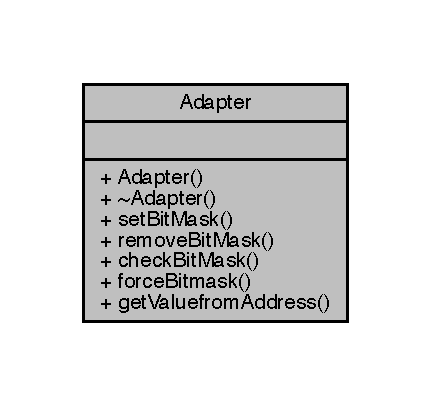
\includegraphics[width=180pt]{class_adapter__coll__graph}
\end{center}
\end{figure}
\subsection*{Öffentliche Methoden}
\begin{DoxyCompactItemize}
\item 
\hyperlink{class_adapter_ae2c6ad0390905b82cac4077642b36620}{Adapter} (uint16\+\_\+t)
\item 
\hyperlink{class_adapter_a08a07acff57eb40aba27455de23ed13c}{$\sim$\+Adapter} ()
\item 
void \hyperlink{class_adapter_adff950a92be7f52dbe08ff3af766a562}{set\+Bit\+Mask} (uint8\+\_\+t bitmask)
\item 
void \hyperlink{class_adapter_a655de45764223d7b1b3847170cc405a5}{remove\+Bit\+Mask} (uint8\+\_\+t bitmask)
\item 
uint8\+\_\+t \hyperlink{class_adapter_a8b1478082798b063a0c04d98fdea06a2}{check\+Bit\+Mask} (uint8\+\_\+t bitmask)
\end{DoxyCompactItemize}


\subsection{Beschreibung der Konstruktoren und Destruktoren}
\hypertarget{class_adapter_ae2c6ad0390905b82cac4077642b36620}{}\label{class_adapter_ae2c6ad0390905b82cac4077642b36620} 
\index{Adapter@{Adapter}!Adapter@{Adapter}}
\index{Adapter@{Adapter}!Adapter@{Adapter}}
\subsubsection{\texorpdfstring{Adapter()}{Adapter()}}
{\footnotesize\ttfamily Adapter\+::\+Adapter (\begin{DoxyParamCaption}\item[{uint16\+\_\+t}]{base }\end{DoxyParamCaption})}

\hypertarget{class_adapter_a08a07acff57eb40aba27455de23ed13c}{}\label{class_adapter_a08a07acff57eb40aba27455de23ed13c} 
\index{Adapter@{Adapter}!````~Adapter@{$\sim$\+Adapter}}
\index{````~Adapter@{$\sim$\+Adapter}!Adapter@{Adapter}}
\subsubsection{\texorpdfstring{$\sim$\+Adapter()}{~Adapter()}}
{\footnotesize\ttfamily Adapter\+::$\sim$\+Adapter (\begin{DoxyParamCaption}{ }\end{DoxyParamCaption})}



\subsection{Dokumentation der Elementfunktionen}
\hypertarget{class_adapter_a8b1478082798b063a0c04d98fdea06a2}{}\label{class_adapter_a8b1478082798b063a0c04d98fdea06a2} 
\index{Adapter@{Adapter}!check\+Bit\+Mask@{check\+Bit\+Mask}}
\index{check\+Bit\+Mask@{check\+Bit\+Mask}!Adapter@{Adapter}}
\subsubsection{\texorpdfstring{check\+Bit\+Mask()}{checkBitMask()}}
{\footnotesize\ttfamily uint8\+\_\+t Adapter\+::check\+Bit\+Mask (\begin{DoxyParamCaption}\item[{uint8\+\_\+t}]{bitmask }\end{DoxyParamCaption})}

\hypertarget{class_adapter_a655de45764223d7b1b3847170cc405a5}{}\label{class_adapter_a655de45764223d7b1b3847170cc405a5} 
\index{Adapter@{Adapter}!remove\+Bit\+Mask@{remove\+Bit\+Mask}}
\index{remove\+Bit\+Mask@{remove\+Bit\+Mask}!Adapter@{Adapter}}
\subsubsection{\texorpdfstring{remove\+Bit\+Mask()}{removeBitMask()}}
{\footnotesize\ttfamily void Adapter\+::remove\+Bit\+Mask (\begin{DoxyParamCaption}\item[{uint8\+\_\+t}]{bitmask }\end{DoxyParamCaption})}

\hypertarget{class_adapter_adff950a92be7f52dbe08ff3af766a562}{}\label{class_adapter_adff950a92be7f52dbe08ff3af766a562} 
\index{Adapter@{Adapter}!set\+Bit\+Mask@{set\+Bit\+Mask}}
\index{set\+Bit\+Mask@{set\+Bit\+Mask}!Adapter@{Adapter}}
\subsubsection{\texorpdfstring{set\+Bit\+Mask()}{setBitMask()}}
{\footnotesize\ttfamily void Adapter\+::set\+Bit\+Mask (\begin{DoxyParamCaption}\item[{uint8\+\_\+t}]{bitmask }\end{DoxyParamCaption})}



Die Dokumentation für diese Klasse wurde erzeugt aufgrund der Dateien\+:\begin{DoxyCompactItemize}
\item 
/\+Users/marvin/conveyor/\+Projekt/\+Hal/\hyperlink{_adapter_8h}{Adapter.\+h}\item 
/\+Users/marvin/conveyor/\+Projekt/\+Hal/\hyperlink{_adapter_8cpp}{Adapter.\+cpp}\end{DoxyCompactItemize}

\hypertarget{class_altimetry}{}\section{Altimetry Klassenreferenz}
\label{class_altimetry}\index{Altimetry@{Altimetry}}


{\ttfamily \#include $<$Altimetry.\+h$>$}



Zusammengehörigkeiten von Altimetry\+:\nopagebreak
\begin{figure}[H]
\begin{center}
\leavevmode
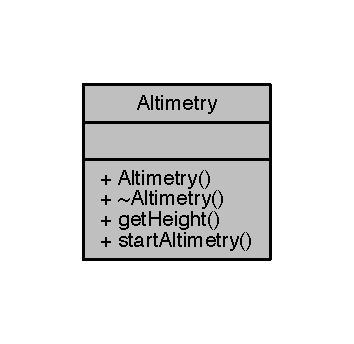
\includegraphics[width=170pt]{class_altimetry__coll__graph}
\end{center}
\end{figure}
\subsection*{Öffentliche Methoden}
\begin{DoxyCompactItemize}
\item 
\hyperlink{class_altimetry_a1a9cb83c86405f07f1bc98ee0d22d65f}{Altimetry} (\hyperlink{class_adapter}{Adapter} $\ast$adapt)
\item 
virtual \hyperlink{class_altimetry_a242b63ebcecf578d9cbc0b80d30bbc2f}{$\sim$\+Altimetry} ()
\item 
uint16\+\_\+t \hyperlink{class_altimetry_a502ab1622b12f938ca61dc40d6a15e07}{get\+Height} ()
\item 
void \hyperlink{class_altimetry_acf39bd22b3d28f8bd41828d2faec3440}{start\+Altimetry} ()
\end{DoxyCompactItemize}


\subsection{Beschreibung der Konstruktoren und Destruktoren}
\hypertarget{class_altimetry_a1a9cb83c86405f07f1bc98ee0d22d65f}{}\label{class_altimetry_a1a9cb83c86405f07f1bc98ee0d22d65f} 
\index{Altimetry@{Altimetry}!Altimetry@{Altimetry}}
\index{Altimetry@{Altimetry}!Altimetry@{Altimetry}}
\subsubsection{\texorpdfstring{Altimetry()}{Altimetry()}}
{\footnotesize\ttfamily Altimetry\+::\+Altimetry (\begin{DoxyParamCaption}\item[{\hyperlink{class_adapter}{Adapter} $\ast$}]{adapt }\end{DoxyParamCaption})}

Constructor der Ampel


\begin{DoxyParams}{Parameter}
{\em adapt} & \hyperlink{class_adapter}{Adapter} für die Steuerung der Ampel. \\
\hline
\end{DoxyParams}
\hypertarget{class_altimetry_a242b63ebcecf578d9cbc0b80d30bbc2f}{}\label{class_altimetry_a242b63ebcecf578d9cbc0b80d30bbc2f} 
\index{Altimetry@{Altimetry}!````~Altimetry@{$\sim$\+Altimetry}}
\index{````~Altimetry@{$\sim$\+Altimetry}!Altimetry@{Altimetry}}
\subsubsection{\texorpdfstring{$\sim$\+Altimetry()}{~Altimetry()}}
{\footnotesize\ttfamily Altimetry\+::$\sim$\+Altimetry (\begin{DoxyParamCaption}{ }\end{DoxyParamCaption})\hspace{0.3cm}{\ttfamily [virtual]}}

Constructor der Ampel


\begin{DoxyParams}{Parameter}
{\em adapt} & \hyperlink{class_adapter}{Adapter} für die Steuerung der Ampel. \\
\hline
\end{DoxyParams}


\subsection{Dokumentation der Elementfunktionen}
\hypertarget{class_altimetry_a502ab1622b12f938ca61dc40d6a15e07}{}\label{class_altimetry_a502ab1622b12f938ca61dc40d6a15e07} 
\index{Altimetry@{Altimetry}!get\+Height@{get\+Height}}
\index{get\+Height@{get\+Height}!Altimetry@{Altimetry}}
\subsubsection{\texorpdfstring{get\+Height()}{getHeight()}}
{\footnotesize\ttfamily uint16\+\_\+t Altimetry\+::get\+Height (\begin{DoxyParamCaption}{ }\end{DoxyParamCaption})}

Oeffnet den .

\begin{DoxyReturn}{Rückgabe}
Gibt Konstant 0 zurueck. 
\end{DoxyReturn}
\hypertarget{class_altimetry_acf39bd22b3d28f8bd41828d2faec3440}{}\label{class_altimetry_acf39bd22b3d28f8bd41828d2faec3440} 
\index{Altimetry@{Altimetry}!start\+Altimetry@{start\+Altimetry}}
\index{start\+Altimetry@{start\+Altimetry}!Altimetry@{Altimetry}}
\subsubsection{\texorpdfstring{start\+Altimetry()}{startAltimetry()}}
{\footnotesize\ttfamily void Altimetry\+::start\+Altimetry (\begin{DoxyParamCaption}{ }\end{DoxyParamCaption})}

Oeffnet den .

\begin{DoxyReturn}{Rückgabe}
Gibt Konstant 0 zurueck. 
\end{DoxyReturn}


Die Dokumentation für diese Klasse wurde erzeugt aufgrund der Dateien\+:\begin{DoxyCompactItemize}
\item 
Hal/\hyperlink{_altimetry_8h}{Altimetry.\+h}\item 
Hal/\hyperlink{_altimetry_8cpp}{Altimetry.\+cpp}\end{DoxyCompactItemize}

\hypertarget{class_config_file}{}\section{Config\+File Klassenreferenz}
\label{class_config_file}\index{Config\+File@{Config\+File}}


{\ttfamily \#include $<$Config\+File.\+h$>$}



Zusammengehörigkeiten von Config\+File\+:\nopagebreak
\begin{figure}[H]
\begin{center}
\leavevmode
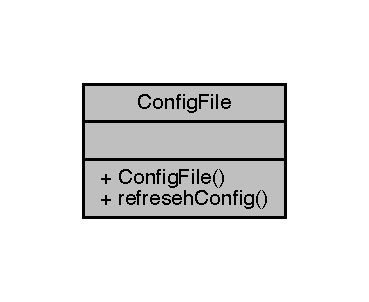
\includegraphics[width=177pt]{class_config_file__coll__graph}
\end{center}
\end{figure}
\subsection*{Öffentliche Methoden}
\begin{DoxyCompactItemize}
\item 
\hyperlink{class_config_file_ab61f21b62426fa46dc4c581d3fdf4e5e}{Config\+File} (std\+::string const \&config\+File)
\item 
void \hyperlink{class_config_file_a48a2e1c781af3f0947c93d1d37e5b71a}{refreseh\+Config} ()
\end{DoxyCompactItemize}


\subsection{Beschreibung der Konstruktoren und Destruktoren}
\hypertarget{class_config_file_ab61f21b62426fa46dc4c581d3fdf4e5e}{}\label{class_config_file_ab61f21b62426fa46dc4c581d3fdf4e5e} 
\index{Config\+File@{Config\+File}!Config\+File@{Config\+File}}
\index{Config\+File@{Config\+File}!Config\+File@{Config\+File}}
\subsubsection{\texorpdfstring{Config\+File()}{ConfigFile()}}
{\footnotesize\ttfamily Config\+File\+::\+Config\+File (\begin{DoxyParamCaption}\item[{std\+::string const \&}]{config\+File }\end{DoxyParamCaption})}



\subsection{Dokumentation der Elementfunktionen}
\hypertarget{class_config_file_a48a2e1c781af3f0947c93d1d37e5b71a}{}\label{class_config_file_a48a2e1c781af3f0947c93d1d37e5b71a} 
\index{Config\+File@{Config\+File}!refreseh\+Config@{refreseh\+Config}}
\index{refreseh\+Config@{refreseh\+Config}!Config\+File@{Config\+File}}
\subsubsection{\texorpdfstring{refreseh\+Config()}{refresehConfig()}}
{\footnotesize\ttfamily void Config\+File\+::refreseh\+Config (\begin{DoxyParamCaption}{ }\end{DoxyParamCaption})}



Die Dokumentation für diese Klasse wurde erzeugt aufgrund der Dateien\+:\begin{DoxyCompactItemize}
\item 
Config\+Management/\hyperlink{_config_file_8h}{Config\+File.\+h}\item 
Config\+Management/\hyperlink{_config_file_8cpp}{Config\+File.\+cpp}\end{DoxyCompactItemize}

\hypertarget{class_config_updater_thread}{}\section{Config\+Updater\+Thread Klassenreferenz}
\label{class_config_updater_thread}\index{Config\+Updater\+Thread@{Config\+Updater\+Thread}}


{\ttfamily \#include $<$Config\+Updater\+Thread.\+h$>$}



Zusammengehörigkeiten von Config\+Updater\+Thread\+:
\nopagebreak
\begin{figure}[H]
\begin{center}
\leavevmode
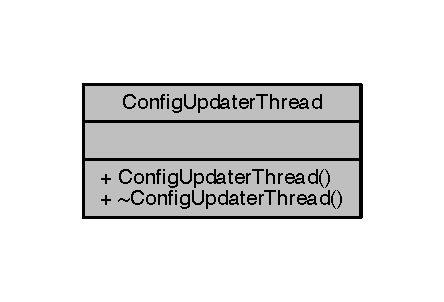
\includegraphics[width=213pt]{class_config_updater_thread__coll__graph}
\end{center}
\end{figure}
\subsection*{Öffentliche Methoden}
\begin{DoxyCompactItemize}
\item 
\hyperlink{class_config_updater_thread_a4ff1049db02d7dba1fff966487689fac}{Config\+Updater\+Thread} ()
\item 
virtual \hyperlink{class_config_updater_thread_a76b9050ee3e35fc85fd1b12eb2cb3ca4}{$\sim$\+Config\+Updater\+Thread} ()
\end{DoxyCompactItemize}


\subsection{Beschreibung der Konstruktoren und Destruktoren}
\hypertarget{class_config_updater_thread_a4ff1049db02d7dba1fff966487689fac}{}\label{class_config_updater_thread_a4ff1049db02d7dba1fff966487689fac} 
\index{Config\+Updater\+Thread@{Config\+Updater\+Thread}!Config\+Updater\+Thread@{Config\+Updater\+Thread}}
\index{Config\+Updater\+Thread@{Config\+Updater\+Thread}!Config\+Updater\+Thread@{Config\+Updater\+Thread}}
\subsubsection{\texorpdfstring{Config\+Updater\+Thread()}{ConfigUpdaterThread()}}
{\footnotesize\ttfamily Config\+Updater\+Thread\+::\+Config\+Updater\+Thread (\begin{DoxyParamCaption}{ }\end{DoxyParamCaption})}

\hypertarget{class_config_updater_thread_a76b9050ee3e35fc85fd1b12eb2cb3ca4}{}\label{class_config_updater_thread_a76b9050ee3e35fc85fd1b12eb2cb3ca4} 
\index{Config\+Updater\+Thread@{Config\+Updater\+Thread}!````~Config\+Updater\+Thread@{$\sim$\+Config\+Updater\+Thread}}
\index{````~Config\+Updater\+Thread@{$\sim$\+Config\+Updater\+Thread}!Config\+Updater\+Thread@{Config\+Updater\+Thread}}
\subsubsection{\texorpdfstring{$\sim$\+Config\+Updater\+Thread()}{~ConfigUpdaterThread()}}
{\footnotesize\ttfamily Config\+Updater\+Thread\+::$\sim$\+Config\+Updater\+Thread (\begin{DoxyParamCaption}{ }\end{DoxyParamCaption})\hspace{0.3cm}{\ttfamily [virtual]}}



Die Dokumentation für diese Klasse wurde erzeugt aufgrund der Dateien\+:\begin{DoxyCompactItemize}
\item 
/\+Users/marvin/conveyor/\+Projekt/\+Thread/\hyperlink{_config_updater_thread_8h}{Config\+Updater\+Thread.\+h}\item 
/\+Users/marvin/conveyor/\+Projekt/\+Thread/\hyperlink{_config_updater_thread_8cpp}{Config\+Updater\+Thread.\+cpp}\end{DoxyCompactItemize}

\hypertarget{class_context}{}\section{Context Klassenreferenz}
\label{class_context}\index{Context@{Context}}


{\ttfamily \#include $<$Context.\+h$>$}



Zusammengehörigkeiten von Context\+:\nopagebreak
\begin{figure}[H]
\begin{center}
\leavevmode
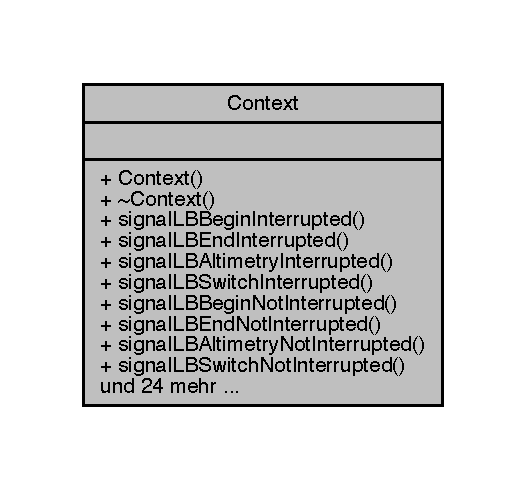
\includegraphics[width=252pt]{class_context__coll__graph}
\end{center}
\end{figure}
\subsection*{Öffentliche Methoden}
\begin{DoxyCompactItemize}
\item 
\hyperlink{class_context_a652cdcd2eedc8dbd9110bd284c5d5cf0}{Context} ()
\item 
virtual \hyperlink{class_context_a2d34e4556448e40693f61d15e091b604}{$\sim$\+Context} ()
\item 
void \hyperlink{class_context_a08df75859b851d2eca2d8e379214d6b5}{signal\+L\+B\+Begin\+Interrupted} ()
\item 
void \hyperlink{class_context_a9e9d5d85cafe8b295193f01fd2b7a8ee}{signal\+L\+B\+End\+Interrupted} ()
\item 
void \hyperlink{class_context_af78ea1902addcf137e8e7d99431592c6}{signal\+L\+B\+Altimetry\+Interrupted} ()
\item 
void \hyperlink{class_context_afdd121a466cf690038ede9b8c2a04160}{signal\+L\+B\+Switch\+Interrupted} ()
\item 
void \hyperlink{class_context_a9528945480d5072126031a6ce0d20b99}{signal\+L\+B\+Begin\+Not\+Interrupted} ()
\item 
void \hyperlink{class_context_a6debf81836f13909119658b40e32fe1c}{signal\+L\+B\+End\+Not\+Interrupted} ()
\item 
void \hyperlink{class_context_acf97db4d70e7246a1d06e4166ece5de5}{signal\+L\+B\+Altimetry\+Not\+Interrupted} ()
\item 
void \hyperlink{class_context_a4fd603eec47acc8a3671b7bdd3bdfe6d}{signal\+L\+B\+Switch\+Not\+Interrupted} ()
\item 
void \hyperlink{class_context_a18bc1a709e3db9477e133f545f7cf66a}{signal\+E\+Stop} ()
\item 
void \hyperlink{class_context_a9fbe4299614bae2f11e92ed56cde640c}{signal\+Start} ()
\item 
void \hyperlink{class_context_ac729f3e2184382006588a438622f235f}{signal\+Stop} ()
\item 
void \hyperlink{class_context_a59ea683658907374dbe23125c11b1e93}{signal\+Reset} ()
\item 
void \hyperlink{class_context_a41c95a05dffe3e6d89ebe5a6522e3a6a}{signal\+L\+B\+Skid\+Interrupted} ()
\item 
void \hyperlink{class_context_a54d07729fce18877b7fa671e5622c2cd}{signal\+L\+B\+Skid\+Not\+Interrupted} ()
\item 
void \hyperlink{class_context_a01e833c79e6ca0d21b419b3f6af9bbdc}{signal\+Altimetry\+Completed} ()
\item 
\hyperlink{class_context_a652cdcd2eedc8dbd9110bd284c5d5cf0}{Context} ()
\item 
virtual \hyperlink{class_context_a8be937c21e267c8d55decced9d1bcf90}{$\sim$\+Context} ()
\item 
void \hyperlink{class_context_a08df75859b851d2eca2d8e379214d6b5}{signal\+L\+B\+Begin\+Interrupted} ()
\item 
void \hyperlink{class_context_a9e9d5d85cafe8b295193f01fd2b7a8ee}{signal\+L\+B\+End\+Interrupted} ()
\item 
void \hyperlink{class_context_af78ea1902addcf137e8e7d99431592c6}{signal\+L\+B\+Altimetry\+Interrupted} ()
\item 
void \hyperlink{class_context_afdd121a466cf690038ede9b8c2a04160}{signal\+L\+B\+Switch\+Interrupted} ()
\item 
void \hyperlink{class_context_a9528945480d5072126031a6ce0d20b99}{signal\+L\+B\+Begin\+Not\+Interrupted} ()
\item 
void \hyperlink{class_context_a6debf81836f13909119658b40e32fe1c}{signal\+L\+B\+End\+Not\+Interrupted} ()
\item 
void \hyperlink{class_context_acf97db4d70e7246a1d06e4166ece5de5}{signal\+L\+B\+Altimetry\+Not\+Interrupted} ()
\item 
void \hyperlink{class_context_a4fd603eec47acc8a3671b7bdd3bdfe6d}{signal\+L\+B\+Switch\+Not\+Interrupted} ()
\item 
void \hyperlink{class_context_a18bc1a709e3db9477e133f545f7cf66a}{signal\+E\+Stop} ()
\item 
void \hyperlink{class_context_a9fbe4299614bae2f11e92ed56cde640c}{signal\+Start} ()
\item 
void \hyperlink{class_context_ac729f3e2184382006588a438622f235f}{signal\+Stop} ()
\item 
void \hyperlink{class_context_a59ea683658907374dbe23125c11b1e93}{signal\+Reset} ()
\item 
void \hyperlink{class_context_a41c95a05dffe3e6d89ebe5a6522e3a6a}{signal\+L\+B\+Skid\+Interrupted} ()
\item 
void \hyperlink{class_context_a54d07729fce18877b7fa671e5622c2cd}{signal\+L\+B\+Skid\+Not\+Interrupted} ()
\item 
void \hyperlink{class_context_a01e833c79e6ca0d21b419b3f6af9bbdc}{signal\+Altimetry\+Completed} ()
\end{DoxyCompactItemize}


\subsection{Beschreibung der Konstruktoren und Destruktoren}
\hypertarget{class_context_a652cdcd2eedc8dbd9110bd284c5d5cf0}{}\label{class_context_a652cdcd2eedc8dbd9110bd284c5d5cf0} 
\index{Context@{Context}!Context@{Context}}
\index{Context@{Context}!Context@{Context}}
\subsubsection{\texorpdfstring{Context()}{Context()}\hspace{0.1cm}{\footnotesize\ttfamily [1/2]}}
{\footnotesize\ttfamily Context\+::\+Context (\begin{DoxyParamCaption}{ }\end{DoxyParamCaption})}

Constructor des Contexts. \hypertarget{class_context_a2d34e4556448e40693f61d15e091b604}{}\label{class_context_a2d34e4556448e40693f61d15e091b604} 
\index{Context@{Context}!````~Context@{$\sim$\+Context}}
\index{````~Context@{$\sim$\+Context}!Context@{Context}}
\subsubsection{\texorpdfstring{$\sim$\+Context()}{~Context()}\hspace{0.1cm}{\footnotesize\ttfamily [1/2]}}
{\footnotesize\ttfamily Context\+::$\sim$\+Context (\begin{DoxyParamCaption}{ }\end{DoxyParamCaption})\hspace{0.3cm}{\ttfamily [virtual]}}

Destructor des Contexts. \hypertarget{class_context_a652cdcd2eedc8dbd9110bd284c5d5cf0}{}\label{class_context_a652cdcd2eedc8dbd9110bd284c5d5cf0} 
\index{Context@{Context}!Context@{Context}}
\index{Context@{Context}!Context@{Context}}
\subsubsection{\texorpdfstring{Context()}{Context()}\hspace{0.1cm}{\footnotesize\ttfamily [2/2]}}
{\footnotesize\ttfamily Context\+::\+Context (\begin{DoxyParamCaption}{ }\end{DoxyParamCaption})}

\hypertarget{class_context_a8be937c21e267c8d55decced9d1bcf90}{}\label{class_context_a8be937c21e267c8d55decced9d1bcf90} 
\index{Context@{Context}!````~Context@{$\sim$\+Context}}
\index{````~Context@{$\sim$\+Context}!Context@{Context}}
\subsubsection{\texorpdfstring{$\sim$\+Context()}{~Context()}\hspace{0.1cm}{\footnotesize\ttfamily [2/2]}}
{\footnotesize\ttfamily virtual Context\+::$\sim$\+Context (\begin{DoxyParamCaption}{ }\end{DoxyParamCaption})\hspace{0.3cm}{\ttfamily [virtual]}}



\subsection{Dokumentation der Elementfunktionen}
\hypertarget{class_context_a01e833c79e6ca0d21b419b3f6af9bbdc}{}\label{class_context_a01e833c79e6ca0d21b419b3f6af9bbdc} 
\index{Context@{Context}!signal\+Altimetry\+Completed@{signal\+Altimetry\+Completed}}
\index{signal\+Altimetry\+Completed@{signal\+Altimetry\+Completed}!Context@{Context}}
\subsubsection{\texorpdfstring{signal\+Altimetry\+Completed()}{signalAltimetryCompleted()}\hspace{0.1cm}{\footnotesize\ttfamily [1/2]}}
{\footnotesize\ttfamily void Context\+::signal\+Altimetry\+Completed (\begin{DoxyParamCaption}{ }\end{DoxyParamCaption})}

\begin{DoxyRefDesc}{Noch zu erledigen}
\item[\hyperlink{todo__todo000014}{Noch zu erledigen}]Ausstehende implementierung Dokumentieren. \end{DoxyRefDesc}
\hypertarget{class_context_a01e833c79e6ca0d21b419b3f6af9bbdc}{}\label{class_context_a01e833c79e6ca0d21b419b3f6af9bbdc} 
\index{Context@{Context}!signal\+Altimetry\+Completed@{signal\+Altimetry\+Completed}}
\index{signal\+Altimetry\+Completed@{signal\+Altimetry\+Completed}!Context@{Context}}
\subsubsection{\texorpdfstring{signal\+Altimetry\+Completed()}{signalAltimetryCompleted()}\hspace{0.1cm}{\footnotesize\ttfamily [2/2]}}
{\footnotesize\ttfamily void Context\+::signal\+Altimetry\+Completed (\begin{DoxyParamCaption}{ }\end{DoxyParamCaption})}

Constructor des Adapters.


\begin{DoxyParams}{Parameter}
{\em baseaddress} & Die Baseaddress die verwenden werden soll. \\
\hline
\end{DoxyParams}
\hypertarget{class_context_a18bc1a709e3db9477e133f545f7cf66a}{}\label{class_context_a18bc1a709e3db9477e133f545f7cf66a} 
\index{Context@{Context}!signal\+E\+Stop@{signal\+E\+Stop}}
\index{signal\+E\+Stop@{signal\+E\+Stop}!Context@{Context}}
\subsubsection{\texorpdfstring{signal\+E\+Stop()}{signalEStop()}\hspace{0.1cm}{\footnotesize\ttfamily [1/2]}}
{\footnotesize\ttfamily void Context\+::signal\+E\+Stop (\begin{DoxyParamCaption}{ }\end{DoxyParamCaption})}

\begin{DoxyRefDesc}{Noch zu erledigen}
\item[\hyperlink{todo__todo000008}{Noch zu erledigen}]Ausstehende implementierung Dokumentieren. \end{DoxyRefDesc}
\hypertarget{class_context_a18bc1a709e3db9477e133f545f7cf66a}{}\label{class_context_a18bc1a709e3db9477e133f545f7cf66a} 
\index{Context@{Context}!signal\+E\+Stop@{signal\+E\+Stop}}
\index{signal\+E\+Stop@{signal\+E\+Stop}!Context@{Context}}
\subsubsection{\texorpdfstring{signal\+E\+Stop()}{signalEStop()}\hspace{0.1cm}{\footnotesize\ttfamily [2/2]}}
{\footnotesize\ttfamily void Context\+::signal\+E\+Stop (\begin{DoxyParamCaption}{ }\end{DoxyParamCaption})}

Constructor des Adapters.


\begin{DoxyParams}{Parameter}
{\em baseaddress} & Die Baseaddress die verwenden werden soll. \\
\hline
\end{DoxyParams}
\hypertarget{class_context_af78ea1902addcf137e8e7d99431592c6}{}\label{class_context_af78ea1902addcf137e8e7d99431592c6} 
\index{Context@{Context}!signal\+L\+B\+Altimetry\+Interrupted@{signal\+L\+B\+Altimetry\+Interrupted}}
\index{signal\+L\+B\+Altimetry\+Interrupted@{signal\+L\+B\+Altimetry\+Interrupted}!Context@{Context}}
\subsubsection{\texorpdfstring{signal\+L\+B\+Altimetry\+Interrupted()}{signalLBAltimetryInterrupted()}\hspace{0.1cm}{\footnotesize\ttfamily [1/2]}}
{\footnotesize\ttfamily void Context\+::signal\+L\+B\+Altimetry\+Interrupted (\begin{DoxyParamCaption}{ }\end{DoxyParamCaption})}

Constructor des Adapters.


\begin{DoxyParams}{Parameter}
{\em baseaddress} & Die Baseaddress die verwenden werden soll. \\
\hline
\end{DoxyParams}
\hypertarget{class_context_af78ea1902addcf137e8e7d99431592c6}{}\label{class_context_af78ea1902addcf137e8e7d99431592c6} 
\index{Context@{Context}!signal\+L\+B\+Altimetry\+Interrupted@{signal\+L\+B\+Altimetry\+Interrupted}}
\index{signal\+L\+B\+Altimetry\+Interrupted@{signal\+L\+B\+Altimetry\+Interrupted}!Context@{Context}}
\subsubsection{\texorpdfstring{signal\+L\+B\+Altimetry\+Interrupted()}{signalLBAltimetryInterrupted()}\hspace{0.1cm}{\footnotesize\ttfamily [2/2]}}
{\footnotesize\ttfamily void Context\+::signal\+L\+B\+Altimetry\+Interrupted (\begin{DoxyParamCaption}{ }\end{DoxyParamCaption})}

\begin{DoxyRefDesc}{Noch zu erledigen}
\item[\hyperlink{todo__todo000003}{Noch zu erledigen}]Ausstehende implementierung Dokumentieren. \end{DoxyRefDesc}
\hypertarget{class_context_acf97db4d70e7246a1d06e4166ece5de5}{}\label{class_context_acf97db4d70e7246a1d06e4166ece5de5} 
\index{Context@{Context}!signal\+L\+B\+Altimetry\+Not\+Interrupted@{signal\+L\+B\+Altimetry\+Not\+Interrupted}}
\index{signal\+L\+B\+Altimetry\+Not\+Interrupted@{signal\+L\+B\+Altimetry\+Not\+Interrupted}!Context@{Context}}
\subsubsection{\texorpdfstring{signal\+L\+B\+Altimetry\+Not\+Interrupted()}{signalLBAltimetryNotInterrupted()}\hspace{0.1cm}{\footnotesize\ttfamily [1/2]}}
{\footnotesize\ttfamily void Context\+::signal\+L\+B\+Altimetry\+Not\+Interrupted (\begin{DoxyParamCaption}{ }\end{DoxyParamCaption})}

Constructor des Adapters.


\begin{DoxyParams}{Parameter}
{\em baseaddress} & Die Baseaddress die verwenden werden soll. \\
\hline
\end{DoxyParams}
\hypertarget{class_context_acf97db4d70e7246a1d06e4166ece5de5}{}\label{class_context_acf97db4d70e7246a1d06e4166ece5de5} 
\index{Context@{Context}!signal\+L\+B\+Altimetry\+Not\+Interrupted@{signal\+L\+B\+Altimetry\+Not\+Interrupted}}
\index{signal\+L\+B\+Altimetry\+Not\+Interrupted@{signal\+L\+B\+Altimetry\+Not\+Interrupted}!Context@{Context}}
\subsubsection{\texorpdfstring{signal\+L\+B\+Altimetry\+Not\+Interrupted()}{signalLBAltimetryNotInterrupted()}\hspace{0.1cm}{\footnotesize\ttfamily [2/2]}}
{\footnotesize\ttfamily void Context\+::signal\+L\+B\+Altimetry\+Not\+Interrupted (\begin{DoxyParamCaption}{ }\end{DoxyParamCaption})}

Constructor des Adapters.


\begin{DoxyParams}{Parameter}
{\em baseaddress} & Die Baseaddress die verwenden werden soll. \\
\hline
\end{DoxyParams}
\hypertarget{class_context_a08df75859b851d2eca2d8e379214d6b5}{}\label{class_context_a08df75859b851d2eca2d8e379214d6b5} 
\index{Context@{Context}!signal\+L\+B\+Begin\+Interrupted@{signal\+L\+B\+Begin\+Interrupted}}
\index{signal\+L\+B\+Begin\+Interrupted@{signal\+L\+B\+Begin\+Interrupted}!Context@{Context}}
\subsubsection{\texorpdfstring{signal\+L\+B\+Begin\+Interrupted()}{signalLBBeginInterrupted()}\hspace{0.1cm}{\footnotesize\ttfamily [1/2]}}
{\footnotesize\ttfamily void Context\+::signal\+L\+B\+Begin\+Interrupted (\begin{DoxyParamCaption}{ }\end{DoxyParamCaption})}

Constructor des Adapters.


\begin{DoxyParams}{Parameter}
{\em baseaddress} & Die Baseaddress die verwenden werden soll. \\
\hline
\end{DoxyParams}
\hypertarget{class_context_a08df75859b851d2eca2d8e379214d6b5}{}\label{class_context_a08df75859b851d2eca2d8e379214d6b5} 
\index{Context@{Context}!signal\+L\+B\+Begin\+Interrupted@{signal\+L\+B\+Begin\+Interrupted}}
\index{signal\+L\+B\+Begin\+Interrupted@{signal\+L\+B\+Begin\+Interrupted}!Context@{Context}}
\subsubsection{\texorpdfstring{signal\+L\+B\+Begin\+Interrupted()}{signalLBBeginInterrupted()}\hspace{0.1cm}{\footnotesize\ttfamily [2/2]}}
{\footnotesize\ttfamily void Context\+::signal\+L\+B\+Begin\+Interrupted (\begin{DoxyParamCaption}{ }\end{DoxyParamCaption})}

\begin{DoxyRefDesc}{Noch zu erledigen}
\item[\hyperlink{todo__todo000001}{Noch zu erledigen}]Ausstehende implementierung Dokumentieren. \end{DoxyRefDesc}
\hypertarget{class_context_a9528945480d5072126031a6ce0d20b99}{}\label{class_context_a9528945480d5072126031a6ce0d20b99} 
\index{Context@{Context}!signal\+L\+B\+Begin\+Not\+Interrupted@{signal\+L\+B\+Begin\+Not\+Interrupted}}
\index{signal\+L\+B\+Begin\+Not\+Interrupted@{signal\+L\+B\+Begin\+Not\+Interrupted}!Context@{Context}}
\subsubsection{\texorpdfstring{signal\+L\+B\+Begin\+Not\+Interrupted()}{signalLBBeginNotInterrupted()}\hspace{0.1cm}{\footnotesize\ttfamily [1/2]}}
{\footnotesize\ttfamily void Context\+::signal\+L\+B\+Begin\+Not\+Interrupted (\begin{DoxyParamCaption}{ }\end{DoxyParamCaption})}

\begin{DoxyRefDesc}{Noch zu erledigen}
\item[\hyperlink{todo__todo000005}{Noch zu erledigen}]Ausstehende implementierung Dokumentieren. \end{DoxyRefDesc}
\hypertarget{class_context_a9528945480d5072126031a6ce0d20b99}{}\label{class_context_a9528945480d5072126031a6ce0d20b99} 
\index{Context@{Context}!signal\+L\+B\+Begin\+Not\+Interrupted@{signal\+L\+B\+Begin\+Not\+Interrupted}}
\index{signal\+L\+B\+Begin\+Not\+Interrupted@{signal\+L\+B\+Begin\+Not\+Interrupted}!Context@{Context}}
\subsubsection{\texorpdfstring{signal\+L\+B\+Begin\+Not\+Interrupted()}{signalLBBeginNotInterrupted()}\hspace{0.1cm}{\footnotesize\ttfamily [2/2]}}
{\footnotesize\ttfamily void Context\+::signal\+L\+B\+Begin\+Not\+Interrupted (\begin{DoxyParamCaption}{ }\end{DoxyParamCaption})}

Constructor des Adapters.


\begin{DoxyParams}{Parameter}
{\em baseaddress} & Die Baseaddress die verwenden werden soll. \\
\hline
\end{DoxyParams}
\hypertarget{class_context_a9e9d5d85cafe8b295193f01fd2b7a8ee}{}\label{class_context_a9e9d5d85cafe8b295193f01fd2b7a8ee} 
\index{Context@{Context}!signal\+L\+B\+End\+Interrupted@{signal\+L\+B\+End\+Interrupted}}
\index{signal\+L\+B\+End\+Interrupted@{signal\+L\+B\+End\+Interrupted}!Context@{Context}}
\subsubsection{\texorpdfstring{signal\+L\+B\+End\+Interrupted()}{signalLBEndInterrupted()}\hspace{0.1cm}{\footnotesize\ttfamily [1/2]}}
{\footnotesize\ttfamily void Context\+::signal\+L\+B\+End\+Interrupted (\begin{DoxyParamCaption}{ }\end{DoxyParamCaption})}

Constructor des Adapters.


\begin{DoxyParams}{Parameter}
{\em baseaddress} & Die Baseaddress die verwenden werden soll. \\
\hline
\end{DoxyParams}
\hypertarget{class_context_a9e9d5d85cafe8b295193f01fd2b7a8ee}{}\label{class_context_a9e9d5d85cafe8b295193f01fd2b7a8ee} 
\index{Context@{Context}!signal\+L\+B\+End\+Interrupted@{signal\+L\+B\+End\+Interrupted}}
\index{signal\+L\+B\+End\+Interrupted@{signal\+L\+B\+End\+Interrupted}!Context@{Context}}
\subsubsection{\texorpdfstring{signal\+L\+B\+End\+Interrupted()}{signalLBEndInterrupted()}\hspace{0.1cm}{\footnotesize\ttfamily [2/2]}}
{\footnotesize\ttfamily void Context\+::signal\+L\+B\+End\+Interrupted (\begin{DoxyParamCaption}{ }\end{DoxyParamCaption})}

\begin{DoxyRefDesc}{Noch zu erledigen}
\item[\hyperlink{todo__todo000002}{Noch zu erledigen}]Ausstehende implementierung Dokumentieren. \end{DoxyRefDesc}
\hypertarget{class_context_a6debf81836f13909119658b40e32fe1c}{}\label{class_context_a6debf81836f13909119658b40e32fe1c} 
\index{Context@{Context}!signal\+L\+B\+End\+Not\+Interrupted@{signal\+L\+B\+End\+Not\+Interrupted}}
\index{signal\+L\+B\+End\+Not\+Interrupted@{signal\+L\+B\+End\+Not\+Interrupted}!Context@{Context}}
\subsubsection{\texorpdfstring{signal\+L\+B\+End\+Not\+Interrupted()}{signalLBEndNotInterrupted()}\hspace{0.1cm}{\footnotesize\ttfamily [1/2]}}
{\footnotesize\ttfamily void Context\+::signal\+L\+B\+End\+Not\+Interrupted (\begin{DoxyParamCaption}{ }\end{DoxyParamCaption})}

\begin{DoxyRefDesc}{Noch zu erledigen}
\item[\hyperlink{todo__todo000006}{Noch zu erledigen}]Ausstehende implementierung Dokumentieren. \end{DoxyRefDesc}
\hypertarget{class_context_a6debf81836f13909119658b40e32fe1c}{}\label{class_context_a6debf81836f13909119658b40e32fe1c} 
\index{Context@{Context}!signal\+L\+B\+End\+Not\+Interrupted@{signal\+L\+B\+End\+Not\+Interrupted}}
\index{signal\+L\+B\+End\+Not\+Interrupted@{signal\+L\+B\+End\+Not\+Interrupted}!Context@{Context}}
\subsubsection{\texorpdfstring{signal\+L\+B\+End\+Not\+Interrupted()}{signalLBEndNotInterrupted()}\hspace{0.1cm}{\footnotesize\ttfamily [2/2]}}
{\footnotesize\ttfamily void Context\+::signal\+L\+B\+End\+Not\+Interrupted (\begin{DoxyParamCaption}{ }\end{DoxyParamCaption})}

Constructor des Adapters.


\begin{DoxyParams}{Parameter}
{\em baseaddress} & Die Baseaddress die verwenden werden soll. \\
\hline
\end{DoxyParams}
\hypertarget{class_context_a41c95a05dffe3e6d89ebe5a6522e3a6a}{}\label{class_context_a41c95a05dffe3e6d89ebe5a6522e3a6a} 
\index{Context@{Context}!signal\+L\+B\+Skid\+Interrupted@{signal\+L\+B\+Skid\+Interrupted}}
\index{signal\+L\+B\+Skid\+Interrupted@{signal\+L\+B\+Skid\+Interrupted}!Context@{Context}}
\subsubsection{\texorpdfstring{signal\+L\+B\+Skid\+Interrupted()}{signalLBSkidInterrupted()}\hspace{0.1cm}{\footnotesize\ttfamily [1/2]}}
{\footnotesize\ttfamily void Context\+::signal\+L\+B\+Skid\+Interrupted (\begin{DoxyParamCaption}{ }\end{DoxyParamCaption})}

\begin{DoxyRefDesc}{Noch zu erledigen}
\item[\hyperlink{todo__todo000012}{Noch zu erledigen}]Ausstehende implementierung Dokumentieren. \end{DoxyRefDesc}
\hypertarget{class_context_a41c95a05dffe3e6d89ebe5a6522e3a6a}{}\label{class_context_a41c95a05dffe3e6d89ebe5a6522e3a6a} 
\index{Context@{Context}!signal\+L\+B\+Skid\+Interrupted@{signal\+L\+B\+Skid\+Interrupted}}
\index{signal\+L\+B\+Skid\+Interrupted@{signal\+L\+B\+Skid\+Interrupted}!Context@{Context}}
\subsubsection{\texorpdfstring{signal\+L\+B\+Skid\+Interrupted()}{signalLBSkidInterrupted()}\hspace{0.1cm}{\footnotesize\ttfamily [2/2]}}
{\footnotesize\ttfamily void Context\+::signal\+L\+B\+Skid\+Interrupted (\begin{DoxyParamCaption}{ }\end{DoxyParamCaption})}

Constructor des Adapters.


\begin{DoxyParams}{Parameter}
{\em baseaddress} & Die Baseaddress die verwenden werden soll. \\
\hline
\end{DoxyParams}
\hypertarget{class_context_a54d07729fce18877b7fa671e5622c2cd}{}\label{class_context_a54d07729fce18877b7fa671e5622c2cd} 
\index{Context@{Context}!signal\+L\+B\+Skid\+Not\+Interrupted@{signal\+L\+B\+Skid\+Not\+Interrupted}}
\index{signal\+L\+B\+Skid\+Not\+Interrupted@{signal\+L\+B\+Skid\+Not\+Interrupted}!Context@{Context}}
\subsubsection{\texorpdfstring{signal\+L\+B\+Skid\+Not\+Interrupted()}{signalLBSkidNotInterrupted()}\hspace{0.1cm}{\footnotesize\ttfamily [1/2]}}
{\footnotesize\ttfamily void Context\+::signal\+L\+B\+Skid\+Not\+Interrupted (\begin{DoxyParamCaption}{ }\end{DoxyParamCaption})}

\begin{DoxyRefDesc}{Noch zu erledigen}
\item[\hyperlink{todo__todo000013}{Noch zu erledigen}]Ausstehende implementierung Dokumentieren. \end{DoxyRefDesc}
\hypertarget{class_context_a54d07729fce18877b7fa671e5622c2cd}{}\label{class_context_a54d07729fce18877b7fa671e5622c2cd} 
\index{Context@{Context}!signal\+L\+B\+Skid\+Not\+Interrupted@{signal\+L\+B\+Skid\+Not\+Interrupted}}
\index{signal\+L\+B\+Skid\+Not\+Interrupted@{signal\+L\+B\+Skid\+Not\+Interrupted}!Context@{Context}}
\subsubsection{\texorpdfstring{signal\+L\+B\+Skid\+Not\+Interrupted()}{signalLBSkidNotInterrupted()}\hspace{0.1cm}{\footnotesize\ttfamily [2/2]}}
{\footnotesize\ttfamily void Context\+::signal\+L\+B\+Skid\+Not\+Interrupted (\begin{DoxyParamCaption}{ }\end{DoxyParamCaption})}

Constructor des Adapters.


\begin{DoxyParams}{Parameter}
{\em baseaddress} & Die Baseaddress die verwenden werden soll. \\
\hline
\end{DoxyParams}
\hypertarget{class_context_afdd121a466cf690038ede9b8c2a04160}{}\label{class_context_afdd121a466cf690038ede9b8c2a04160} 
\index{Context@{Context}!signal\+L\+B\+Switch\+Interrupted@{signal\+L\+B\+Switch\+Interrupted}}
\index{signal\+L\+B\+Switch\+Interrupted@{signal\+L\+B\+Switch\+Interrupted}!Context@{Context}}
\subsubsection{\texorpdfstring{signal\+L\+B\+Switch\+Interrupted()}{signalLBSwitchInterrupted()}\hspace{0.1cm}{\footnotesize\ttfamily [1/2]}}
{\footnotesize\ttfamily void Context\+::signal\+L\+B\+Switch\+Interrupted (\begin{DoxyParamCaption}{ }\end{DoxyParamCaption})}

Constructor des Adapters.


\begin{DoxyParams}{Parameter}
{\em baseaddress} & Die Baseaddress die verwenden werden soll. \\
\hline
\end{DoxyParams}
\hypertarget{class_context_afdd121a466cf690038ede9b8c2a04160}{}\label{class_context_afdd121a466cf690038ede9b8c2a04160} 
\index{Context@{Context}!signal\+L\+B\+Switch\+Interrupted@{signal\+L\+B\+Switch\+Interrupted}}
\index{signal\+L\+B\+Switch\+Interrupted@{signal\+L\+B\+Switch\+Interrupted}!Context@{Context}}
\subsubsection{\texorpdfstring{signal\+L\+B\+Switch\+Interrupted()}{signalLBSwitchInterrupted()}\hspace{0.1cm}{\footnotesize\ttfamily [2/2]}}
{\footnotesize\ttfamily void Context\+::signal\+L\+B\+Switch\+Interrupted (\begin{DoxyParamCaption}{ }\end{DoxyParamCaption})}

\begin{DoxyRefDesc}{Noch zu erledigen}
\item[\hyperlink{todo__todo000004}{Noch zu erledigen}]Ausstehende implementierung Dokumentieren. \end{DoxyRefDesc}
\hypertarget{class_context_a4fd603eec47acc8a3671b7bdd3bdfe6d}{}\label{class_context_a4fd603eec47acc8a3671b7bdd3bdfe6d} 
\index{Context@{Context}!signal\+L\+B\+Switch\+Not\+Interrupted@{signal\+L\+B\+Switch\+Not\+Interrupted}}
\index{signal\+L\+B\+Switch\+Not\+Interrupted@{signal\+L\+B\+Switch\+Not\+Interrupted}!Context@{Context}}
\subsubsection{\texorpdfstring{signal\+L\+B\+Switch\+Not\+Interrupted()}{signalLBSwitchNotInterrupted()}\hspace{0.1cm}{\footnotesize\ttfamily [1/2]}}
{\footnotesize\ttfamily void Context\+::signal\+L\+B\+Switch\+Not\+Interrupted (\begin{DoxyParamCaption}{ }\end{DoxyParamCaption})}

\begin{DoxyRefDesc}{Noch zu erledigen}
\item[\hyperlink{todo__todo000007}{Noch zu erledigen}]Ausstehende implementierung Dokumentieren. \end{DoxyRefDesc}
\hypertarget{class_context_a4fd603eec47acc8a3671b7bdd3bdfe6d}{}\label{class_context_a4fd603eec47acc8a3671b7bdd3bdfe6d} 
\index{Context@{Context}!signal\+L\+B\+Switch\+Not\+Interrupted@{signal\+L\+B\+Switch\+Not\+Interrupted}}
\index{signal\+L\+B\+Switch\+Not\+Interrupted@{signal\+L\+B\+Switch\+Not\+Interrupted}!Context@{Context}}
\subsubsection{\texorpdfstring{signal\+L\+B\+Switch\+Not\+Interrupted()}{signalLBSwitchNotInterrupted()}\hspace{0.1cm}{\footnotesize\ttfamily [2/2]}}
{\footnotesize\ttfamily void Context\+::signal\+L\+B\+Switch\+Not\+Interrupted (\begin{DoxyParamCaption}{ }\end{DoxyParamCaption})}

Constructor des Adapters.


\begin{DoxyParams}{Parameter}
{\em baseaddress} & Die Baseaddress die verwenden werden soll. \\
\hline
\end{DoxyParams}
\hypertarget{class_context_a59ea683658907374dbe23125c11b1e93}{}\label{class_context_a59ea683658907374dbe23125c11b1e93} 
\index{Context@{Context}!signal\+Reset@{signal\+Reset}}
\index{signal\+Reset@{signal\+Reset}!Context@{Context}}
\subsubsection{\texorpdfstring{signal\+Reset()}{signalReset()}\hspace{0.1cm}{\footnotesize\ttfamily [1/2]}}
{\footnotesize\ttfamily void Context\+::signal\+Reset (\begin{DoxyParamCaption}{ }\end{DoxyParamCaption})}

\begin{DoxyRefDesc}{Noch zu erledigen}
\item[\hyperlink{todo__todo000011}{Noch zu erledigen}]Ausstehende implementierung Dokumentieren. \end{DoxyRefDesc}
\hypertarget{class_context_a59ea683658907374dbe23125c11b1e93}{}\label{class_context_a59ea683658907374dbe23125c11b1e93} 
\index{Context@{Context}!signal\+Reset@{signal\+Reset}}
\index{signal\+Reset@{signal\+Reset}!Context@{Context}}
\subsubsection{\texorpdfstring{signal\+Reset()}{signalReset()}\hspace{0.1cm}{\footnotesize\ttfamily [2/2]}}
{\footnotesize\ttfamily void Context\+::signal\+Reset (\begin{DoxyParamCaption}{ }\end{DoxyParamCaption})}

Constructor des Adapters.


\begin{DoxyParams}{Parameter}
{\em baseaddress} & Die Baseaddress die verwenden werden soll. \\
\hline
\end{DoxyParams}
\hypertarget{class_context_a9fbe4299614bae2f11e92ed56cde640c}{}\label{class_context_a9fbe4299614bae2f11e92ed56cde640c} 
\index{Context@{Context}!signal\+Start@{signal\+Start}}
\index{signal\+Start@{signal\+Start}!Context@{Context}}
\subsubsection{\texorpdfstring{signal\+Start()}{signalStart()}\hspace{0.1cm}{\footnotesize\ttfamily [1/2]}}
{\footnotesize\ttfamily void Context\+::signal\+Start (\begin{DoxyParamCaption}{ }\end{DoxyParamCaption})}

\begin{DoxyRefDesc}{Noch zu erledigen}
\item[\hyperlink{todo__todo000009}{Noch zu erledigen}]Ausstehende implementierung Dokumentieren. \end{DoxyRefDesc}
\hypertarget{class_context_a9fbe4299614bae2f11e92ed56cde640c}{}\label{class_context_a9fbe4299614bae2f11e92ed56cde640c} 
\index{Context@{Context}!signal\+Start@{signal\+Start}}
\index{signal\+Start@{signal\+Start}!Context@{Context}}
\subsubsection{\texorpdfstring{signal\+Start()}{signalStart()}\hspace{0.1cm}{\footnotesize\ttfamily [2/2]}}
{\footnotesize\ttfamily void Context\+::signal\+Start (\begin{DoxyParamCaption}{ }\end{DoxyParamCaption})}

Constructor des Adapters.


\begin{DoxyParams}{Parameter}
{\em baseaddress} & Die Baseaddress die verwenden werden soll. \\
\hline
\end{DoxyParams}
\hypertarget{class_context_ac729f3e2184382006588a438622f235f}{}\label{class_context_ac729f3e2184382006588a438622f235f} 
\index{Context@{Context}!signal\+Stop@{signal\+Stop}}
\index{signal\+Stop@{signal\+Stop}!Context@{Context}}
\subsubsection{\texorpdfstring{signal\+Stop()}{signalStop()}\hspace{0.1cm}{\footnotesize\ttfamily [1/2]}}
{\footnotesize\ttfamily void Context\+::signal\+Stop (\begin{DoxyParamCaption}{ }\end{DoxyParamCaption})}

\begin{DoxyRefDesc}{Noch zu erledigen}
\item[\hyperlink{todo__todo000010}{Noch zu erledigen}]Ausstehende implementierung Dokumentieren. \end{DoxyRefDesc}
\hypertarget{class_context_ac729f3e2184382006588a438622f235f}{}\label{class_context_ac729f3e2184382006588a438622f235f} 
\index{Context@{Context}!signal\+Stop@{signal\+Stop}}
\index{signal\+Stop@{signal\+Stop}!Context@{Context}}
\subsubsection{\texorpdfstring{signal\+Stop()}{signalStop()}\hspace{0.1cm}{\footnotesize\ttfamily [2/2]}}
{\footnotesize\ttfamily void Context\+::signal\+Stop (\begin{DoxyParamCaption}{ }\end{DoxyParamCaption})}

Constructor des Adapters.


\begin{DoxyParams}{Parameter}
{\em baseaddress} & Die Baseaddress die verwenden werden soll. \\
\hline
\end{DoxyParams}


Die Dokumentation für diese Klasse wurde erzeugt aufgrund der Dateien\+:\begin{DoxyCompactItemize}
\item 
F\+S\+M/\hyperlink{_f_s_m_2_context_8h}{Context.\+h}\item 
F\+S\+M/\hyperlink{_f_s_m_2_context_8cpp}{Context.\+cpp}\end{DoxyCompactItemize}

\hypertarget{class_conveyor_one_controller}{}\section{Conveyor\+One\+Controller Klassenreferenz}
\label{class_conveyor_one_controller}\index{Conveyor\+One\+Controller@{Conveyor\+One\+Controller}}


{\ttfamily \#include $<$Conveyor\+One\+Controller.\+h$>$}



Zusammengehörigkeiten von Conveyor\+One\+Controller\+:\nopagebreak
\begin{figure}[H]
\begin{center}
\leavevmode
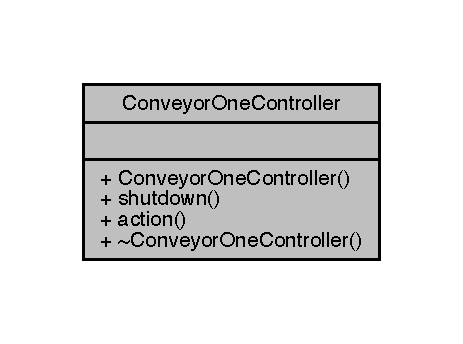
\includegraphics[width=222pt]{class_conveyor_one_controller__coll__graph}
\end{center}
\end{figure}
\subsection*{Öffentliche Methoden}
\begin{DoxyCompactItemize}
\item 
\hyperlink{class_conveyor_one_controller_ab93770638de1fbf75612b8886b48ce83}{Conveyor\+One\+Controller} ()
\item 
void \hyperlink{class_conveyor_one_controller_a837b5b29b5933795413a50446abd9861}{shutdown} ()
\item 
void \hyperlink{class_conveyor_one_controller_a4afc5302a370ec6b1d19514df56ce64c}{action} ()
\item 
virtual \hyperlink{class_conveyor_one_controller_a7e284560fd1dd2b55b38418b3b7e9e16}{$\sim$\+Conveyor\+One\+Controller} ()
\end{DoxyCompactItemize}


\subsection{Beschreibung der Konstruktoren und Destruktoren}
\hypertarget{class_conveyor_one_controller_ab93770638de1fbf75612b8886b48ce83}{}\label{class_conveyor_one_controller_ab93770638de1fbf75612b8886b48ce83} 
\index{Conveyor\+One\+Controller@{Conveyor\+One\+Controller}!Conveyor\+One\+Controller@{Conveyor\+One\+Controller}}
\index{Conveyor\+One\+Controller@{Conveyor\+One\+Controller}!Conveyor\+One\+Controller@{Conveyor\+One\+Controller}}
\subsubsection{\texorpdfstring{Conveyor\+One\+Controller()}{ConveyorOneController()}}
{\footnotesize\ttfamily Conveyor\+One\+Controller\+::\+Conveyor\+One\+Controller (\begin{DoxyParamCaption}{ }\end{DoxyParamCaption})}

\hypertarget{class_conveyor_one_controller_a7e284560fd1dd2b55b38418b3b7e9e16}{}\label{class_conveyor_one_controller_a7e284560fd1dd2b55b38418b3b7e9e16} 
\index{Conveyor\+One\+Controller@{Conveyor\+One\+Controller}!````~Conveyor\+One\+Controller@{$\sim$\+Conveyor\+One\+Controller}}
\index{````~Conveyor\+One\+Controller@{$\sim$\+Conveyor\+One\+Controller}!Conveyor\+One\+Controller@{Conveyor\+One\+Controller}}
\subsubsection{\texorpdfstring{$\sim$\+Conveyor\+One\+Controller()}{~ConveyorOneController()}}
{\footnotesize\ttfamily Conveyor\+One\+Controller\+::$\sim$\+Conveyor\+One\+Controller (\begin{DoxyParamCaption}{ }\end{DoxyParamCaption})\hspace{0.3cm}{\ttfamily [virtual]}}



\subsection{Dokumentation der Elementfunktionen}
\hypertarget{class_conveyor_one_controller_a4afc5302a370ec6b1d19514df56ce64c}{}\label{class_conveyor_one_controller_a4afc5302a370ec6b1d19514df56ce64c} 
\index{Conveyor\+One\+Controller@{Conveyor\+One\+Controller}!action@{action}}
\index{action@{action}!Conveyor\+One\+Controller@{Conveyor\+One\+Controller}}
\subsubsection{\texorpdfstring{action()}{action()}}
{\footnotesize\ttfamily void Conveyor\+One\+Controller\+::action (\begin{DoxyParamCaption}{ }\end{DoxyParamCaption})}

\hypertarget{class_conveyor_one_controller_a837b5b29b5933795413a50446abd9861}{}\label{class_conveyor_one_controller_a837b5b29b5933795413a50446abd9861} 
\index{Conveyor\+One\+Controller@{Conveyor\+One\+Controller}!shutdown@{shutdown}}
\index{shutdown@{shutdown}!Conveyor\+One\+Controller@{Conveyor\+One\+Controller}}
\subsubsection{\texorpdfstring{shutdown()}{shutdown()}}
{\footnotesize\ttfamily void Conveyor\+One\+Controller\+::shutdown (\begin{DoxyParamCaption}{ }\end{DoxyParamCaption})}



Die Dokumentation für diese Klasse wurde erzeugt aufgrund der Dateien\+:\begin{DoxyCompactItemize}
\item 
Controller/\hyperlink{_conveyor_one_controller_8h}{Conveyor\+One\+Controller.\+h}\item 
Controller/\hyperlink{_conveyor_one_controller_8cpp}{Conveyor\+One\+Controller.\+cpp}\end{DoxyCompactItemize}

\hypertarget{class_conveyor_thread}{}\section{Conveyor\+Thread Klassenreferenz}
\label{class_conveyor_thread}\index{Conveyor\+Thread@{Conveyor\+Thread}}


{\ttfamily \#include $<$Conveyor\+Thread.\+h$>$}



Klassendiagramm für Conveyor\+Thread\+:\nopagebreak
\begin{figure}[H]
\begin{center}
\leavevmode
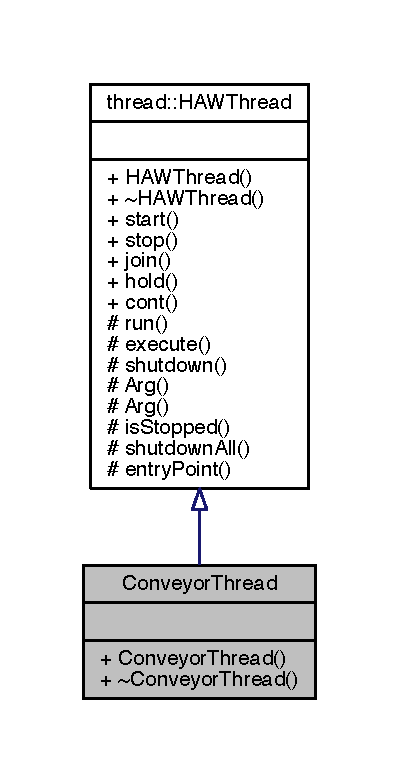
\includegraphics[width=192pt]{class_conveyor_thread__inherit__graph}
\end{center}
\end{figure}


Zusammengehörigkeiten von Conveyor\+Thread\+:\nopagebreak
\begin{figure}[H]
\begin{center}
\leavevmode
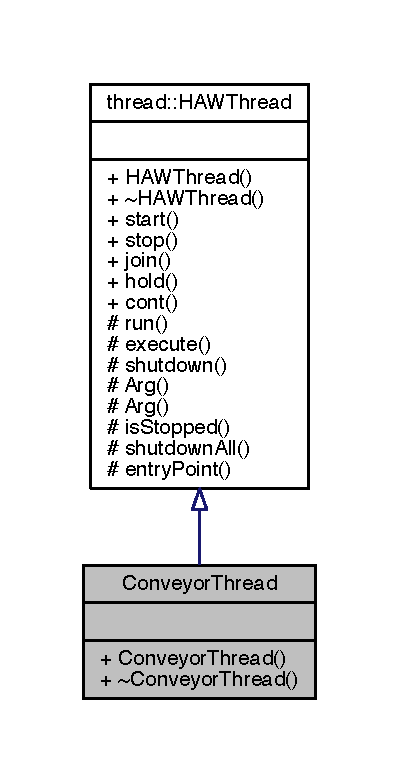
\includegraphics[width=192pt]{class_conveyor_thread__coll__graph}
\end{center}
\end{figure}
\subsection*{Öffentliche Methoden}
\begin{DoxyCompactItemize}
\item 
\hyperlink{class_conveyor_thread_a2068e0741d46acdd2738d65447b594b6}{Conveyor\+Thread} ()
\item 
virtual \hyperlink{class_conveyor_thread_ac496ae2a4708c7cd3af20721c1bf8b8a}{$\sim$\+Conveyor\+Thread} ()
\end{DoxyCompactItemize}
\subsection*{Weitere Geerbte Elemente}


\subsection{Beschreibung der Konstruktoren und Destruktoren}
\hypertarget{class_conveyor_thread_a2068e0741d46acdd2738d65447b594b6}{}\label{class_conveyor_thread_a2068e0741d46acdd2738d65447b594b6} 
\index{Conveyor\+Thread@{Conveyor\+Thread}!Conveyor\+Thread@{Conveyor\+Thread}}
\index{Conveyor\+Thread@{Conveyor\+Thread}!Conveyor\+Thread@{Conveyor\+Thread}}
\subsubsection{\texorpdfstring{Conveyor\+Thread()}{ConveyorThread()}}
{\footnotesize\ttfamily Conveyor\+Thread\+::\+Conveyor\+Thread (\begin{DoxyParamCaption}{ }\end{DoxyParamCaption})}

\hypertarget{class_conveyor_thread_ac496ae2a4708c7cd3af20721c1bf8b8a}{}\label{class_conveyor_thread_ac496ae2a4708c7cd3af20721c1bf8b8a} 
\index{Conveyor\+Thread@{Conveyor\+Thread}!````~Conveyor\+Thread@{$\sim$\+Conveyor\+Thread}}
\index{````~Conveyor\+Thread@{$\sim$\+Conveyor\+Thread}!Conveyor\+Thread@{Conveyor\+Thread}}
\subsubsection{\texorpdfstring{$\sim$\+Conveyor\+Thread()}{~ConveyorThread()}}
{\footnotesize\ttfamily Conveyor\+Thread\+::$\sim$\+Conveyor\+Thread (\begin{DoxyParamCaption}{ }\end{DoxyParamCaption})\hspace{0.3cm}{\ttfamily [virtual]}}



Die Dokumentation für diese Klasse wurde erzeugt aufgrund der Dateien\+:\begin{DoxyCompactItemize}
\item 
Thread/\hyperlink{_conveyor_thread_8h}{Conveyor\+Thread.\+h}\item 
Thread/\hyperlink{_conveyor_thread_8cpp}{Conveyor\+Thread.\+cpp}\end{DoxyCompactItemize}

\hypertarget{class_conveyor_three_controller}{}\section{Conveyor\+Three\+Controller Klassenreferenz}
\label{class_conveyor_three_controller}\index{Conveyor\+Three\+Controller@{Conveyor\+Three\+Controller}}


{\ttfamily \#include $<$Conveyor\+Three\+Controller.\+h$>$}



Zusammengehörigkeiten von Conveyor\+Three\+Controller\+:
\nopagebreak
\begin{figure}[H]
\begin{center}
\leavevmode
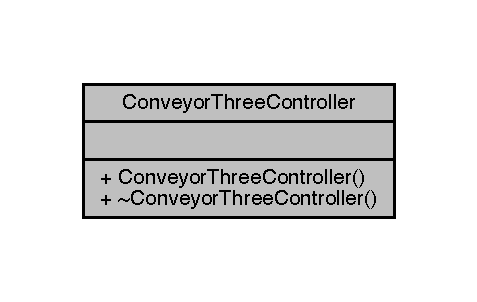
\includegraphics[width=229pt]{class_conveyor_three_controller__coll__graph}
\end{center}
\end{figure}
\subsection*{Öffentliche Methoden}
\begin{DoxyCompactItemize}
\item 
\hyperlink{class_conveyor_three_controller_ad35c62e9764dc39314521c3b7e451eb4}{Conveyor\+Three\+Controller} ()
\item 
virtual \hyperlink{class_conveyor_three_controller_a3ea9a30cb49da76384b3633d11240c92}{$\sim$\+Conveyor\+Three\+Controller} ()
\end{DoxyCompactItemize}


\subsection{Beschreibung der Konstruktoren und Destruktoren}
\hypertarget{class_conveyor_three_controller_ad35c62e9764dc39314521c3b7e451eb4}{}\label{class_conveyor_three_controller_ad35c62e9764dc39314521c3b7e451eb4} 
\index{Conveyor\+Three\+Controller@{Conveyor\+Three\+Controller}!Conveyor\+Three\+Controller@{Conveyor\+Three\+Controller}}
\index{Conveyor\+Three\+Controller@{Conveyor\+Three\+Controller}!Conveyor\+Three\+Controller@{Conveyor\+Three\+Controller}}
\subsubsection{\texorpdfstring{Conveyor\+Three\+Controller()}{ConveyorThreeController()}}
{\footnotesize\ttfamily Conveyor\+Three\+Controller\+::\+Conveyor\+Three\+Controller (\begin{DoxyParamCaption}{ }\end{DoxyParamCaption})}

\hypertarget{class_conveyor_three_controller_a3ea9a30cb49da76384b3633d11240c92}{}\label{class_conveyor_three_controller_a3ea9a30cb49da76384b3633d11240c92} 
\index{Conveyor\+Three\+Controller@{Conveyor\+Three\+Controller}!````~Conveyor\+Three\+Controller@{$\sim$\+Conveyor\+Three\+Controller}}
\index{````~Conveyor\+Three\+Controller@{$\sim$\+Conveyor\+Three\+Controller}!Conveyor\+Three\+Controller@{Conveyor\+Three\+Controller}}
\subsubsection{\texorpdfstring{$\sim$\+Conveyor\+Three\+Controller()}{~ConveyorThreeController()}}
{\footnotesize\ttfamily Conveyor\+Three\+Controller\+::$\sim$\+Conveyor\+Three\+Controller (\begin{DoxyParamCaption}{ }\end{DoxyParamCaption})\hspace{0.3cm}{\ttfamily [virtual]}}



Die Dokumentation für diese Klasse wurde erzeugt aufgrund der Dateien\+:\begin{DoxyCompactItemize}
\item 
/\+Users/marvin/conveyor/\+Projekt/\+Controller/\hyperlink{_conveyor_three_controller_8h}{Conveyor\+Three\+Controller.\+h}\item 
/\+Users/marvin/conveyor/\+Projekt/\+Controller/\hyperlink{_conveyor_three_controller_8cpp}{Conveyor\+Three\+Controller.\+cpp}\end{DoxyCompactItemize}

\hypertarget{class_conveyor_two_controller}{}\section{Conveyor\+Two\+Controller Klassenreferenz}
\label{class_conveyor_two_controller}\index{Conveyor\+Two\+Controller@{Conveyor\+Two\+Controller}}


{\ttfamily \#include $<$Conveyor\+Two\+Controller.\+h$>$}



Zusammengehörigkeiten von Conveyor\+Two\+Controller\+:\nopagebreak
\begin{figure}[H]
\begin{center}
\leavevmode
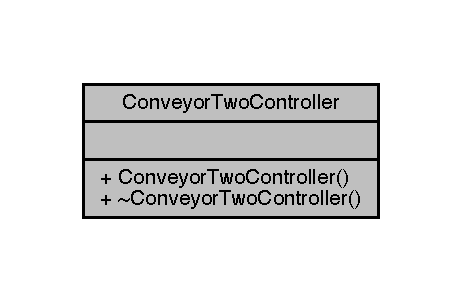
\includegraphics[width=222pt]{class_conveyor_two_controller__coll__graph}
\end{center}
\end{figure}
\subsection*{Öffentliche Methoden}
\begin{DoxyCompactItemize}
\item 
\hyperlink{class_conveyor_two_controller_abf1818572c62c90a086af7b92116d91c}{Conveyor\+Two\+Controller} ()
\item 
virtual \hyperlink{class_conveyor_two_controller_a7b2d996e62a8467455279ce295b5c889}{$\sim$\+Conveyor\+Two\+Controller} ()
\end{DoxyCompactItemize}


\subsection{Beschreibung der Konstruktoren und Destruktoren}
\hypertarget{class_conveyor_two_controller_abf1818572c62c90a086af7b92116d91c}{}\label{class_conveyor_two_controller_abf1818572c62c90a086af7b92116d91c} 
\index{Conveyor\+Two\+Controller@{Conveyor\+Two\+Controller}!Conveyor\+Two\+Controller@{Conveyor\+Two\+Controller}}
\index{Conveyor\+Two\+Controller@{Conveyor\+Two\+Controller}!Conveyor\+Two\+Controller@{Conveyor\+Two\+Controller}}
\subsubsection{\texorpdfstring{Conveyor\+Two\+Controller()}{ConveyorTwoController()}}
{\footnotesize\ttfamily Conveyor\+Two\+Controller\+::\+Conveyor\+Two\+Controller (\begin{DoxyParamCaption}{ }\end{DoxyParamCaption})}

\hypertarget{class_conveyor_two_controller_a7b2d996e62a8467455279ce295b5c889}{}\label{class_conveyor_two_controller_a7b2d996e62a8467455279ce295b5c889} 
\index{Conveyor\+Two\+Controller@{Conveyor\+Two\+Controller}!````~Conveyor\+Two\+Controller@{$\sim$\+Conveyor\+Two\+Controller}}
\index{````~Conveyor\+Two\+Controller@{$\sim$\+Conveyor\+Two\+Controller}!Conveyor\+Two\+Controller@{Conveyor\+Two\+Controller}}
\subsubsection{\texorpdfstring{$\sim$\+Conveyor\+Two\+Controller()}{~ConveyorTwoController()}}
{\footnotesize\ttfamily Conveyor\+Two\+Controller\+::$\sim$\+Conveyor\+Two\+Controller (\begin{DoxyParamCaption}{ }\end{DoxyParamCaption})\hspace{0.3cm}{\ttfamily [virtual]}}



Die Dokumentation für diese Klasse wurde erzeugt aufgrund der Dateien\+:\begin{DoxyCompactItemize}
\item 
Controller/\hyperlink{_conveyor_two_controller_8h}{Conveyor\+Two\+Controller.\+h}\item 
Controller/\hyperlink{_conveyor_two_controller_8cpp}{Conveyor\+Two\+Controller.\+cpp}\end{DoxyCompactItemize}

\hypertarget{class_hal_builder}{}\section{Hal\+Builder Klassenreferenz}
\label{class_hal_builder}\index{Hal\+Builder@{Hal\+Builder}}


{\ttfamily \#include $<$Hal\+Builder.\+h$>$}



Zusammengehörigkeiten von Hal\+Builder\+:\nopagebreak
\begin{figure}[H]
\begin{center}
\leavevmode
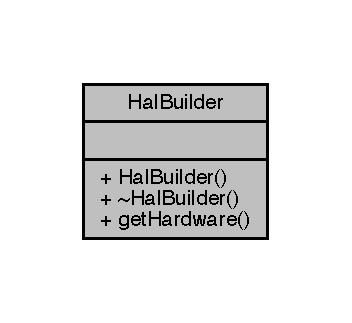
\includegraphics[width=169pt]{class_hal_builder__coll__graph}
\end{center}
\end{figure}
\subsection*{Öffentliche Methoden}
\begin{DoxyCompactItemize}
\item 
\hyperlink{class_hal_builder_a722e3025d6c9659efcc011df559d0619}{Hal\+Builder} ()
\item 
\hyperlink{class_hardware}{Hardware} $\ast$ \hyperlink{class_hal_builder_addc8f400dfa9dee3f0d9de116512212f}{get\+Hardware} ()
\item 
virtual \hyperlink{class_hal_builder_af77e28e213c8aa028b18cf435e9ef3c8}{$\sim$\+Hal\+Builder} ()
\end{DoxyCompactItemize}


\subsection{Beschreibung der Konstruktoren und Destruktoren}
\hypertarget{class_hal_builder_a722e3025d6c9659efcc011df559d0619}{}\label{class_hal_builder_a722e3025d6c9659efcc011df559d0619} 
\index{Hal\+Builder@{Hal\+Builder}!Hal\+Builder@{Hal\+Builder}}
\index{Hal\+Builder@{Hal\+Builder}!Hal\+Builder@{Hal\+Builder}}
\subsubsection{\texorpdfstring{Hal\+Builder()}{HalBuilder()}}
{\footnotesize\ttfamily Hal\+Builder\+::\+Hal\+Builder (\begin{DoxyParamCaption}{ }\end{DoxyParamCaption})}

\hypertarget{class_hal_builder_af77e28e213c8aa028b18cf435e9ef3c8}{}\label{class_hal_builder_af77e28e213c8aa028b18cf435e9ef3c8} 
\index{Hal\+Builder@{Hal\+Builder}!````~Hal\+Builder@{$\sim$\+Hal\+Builder}}
\index{````~Hal\+Builder@{$\sim$\+Hal\+Builder}!Hal\+Builder@{Hal\+Builder}}
\subsubsection{\texorpdfstring{$\sim$\+Hal\+Builder()}{~HalBuilder()}}
{\footnotesize\ttfamily Hal\+Builder\+::$\sim$\+Hal\+Builder (\begin{DoxyParamCaption}{ }\end{DoxyParamCaption})\hspace{0.3cm}{\ttfamily [virtual]}}



\subsection{Dokumentation der Elementfunktionen}
\hypertarget{class_hal_builder_addc8f400dfa9dee3f0d9de116512212f}{}\label{class_hal_builder_addc8f400dfa9dee3f0d9de116512212f} 
\index{Hal\+Builder@{Hal\+Builder}!get\+Hardware@{get\+Hardware}}
\index{get\+Hardware@{get\+Hardware}!Hal\+Builder@{Hal\+Builder}}
\subsubsection{\texorpdfstring{get\+Hardware()}{getHardware()}}
{\footnotesize\ttfamily \hyperlink{class_hardware}{Hardware} $\ast$ Hal\+Builder\+::get\+Hardware (\begin{DoxyParamCaption}{ }\end{DoxyParamCaption})}



Die Dokumentation für diese Klasse wurde erzeugt aufgrund der Dateien\+:\begin{DoxyCompactItemize}
\item 
Hal/\hyperlink{_hal_builder_8h}{Hal\+Builder.\+h}\item 
Hal/\hyperlink{_hal_builder_8cpp}{Hal\+Builder.\+cpp}\end{DoxyCompactItemize}

\hypertarget{class_hardware}{}\section{Hardware Klassenreferenz}
\label{class_hardware}\index{Hardware@{Hardware}}


{\ttfamily \#include $<$Hardware.\+h$>$}



Zusammengehörigkeiten von Hardware\+:
\nopagebreak
\begin{figure}[H]
\begin{center}
\leavevmode
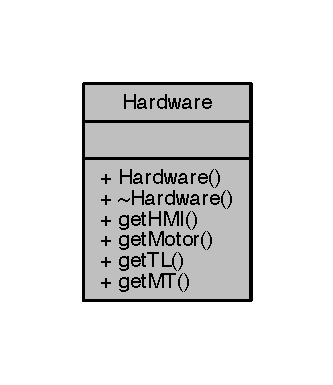
\includegraphics[width=160pt]{class_hardware__coll__graph}
\end{center}
\end{figure}
\subsection*{Öffentliche Methoden}
\begin{DoxyCompactItemize}
\item 
\hyperlink{class_hardware_a554fd479b788d6d73473aceb117f17d8}{Hardware} (\hyperlink{class_human_machine_interface}{Human\+Machine\+Interface} $\ast$hmi, \hyperlink{class_motor}{Motor} $\ast$motor, \hyperlink{class_traffic_light}{Traffic\+Light} $\ast$tl, \hyperlink{class_measuring_tool}{Measuring\+Tool} $\ast$mt)
\item 
\hyperlink{class_hardware_a92901a44130552d28485409bcf6906f5}{$\sim$\+Hardware} ()
\item 
\hyperlink{class_human_machine_interface}{Human\+Machine\+Interface} $\ast$ \hyperlink{class_hardware_aec8f013270ef5d6e79afed214b5c18cf}{get\+H\+MI} ()
\item 
\hyperlink{class_motor}{Motor} $\ast$ \hyperlink{class_hardware_a0a896143b14292ea1805d43e384b4fa1}{get\+Motor} ()
\item 
\hyperlink{class_traffic_light}{Traffic\+Light} $\ast$ \hyperlink{class_hardware_a558325fc00a829ca20112234a961b153}{get\+TL} ()
\item 
\hyperlink{class_measuring_tool}{Measuring\+Tool} $\ast$ \hyperlink{class_hardware_a6acc1b03b3c39ddbd681058f49e9f1bd}{get\+MT} ()
\end{DoxyCompactItemize}


\subsection{Beschreibung der Konstruktoren und Destruktoren}
\hypertarget{class_hardware_a554fd479b788d6d73473aceb117f17d8}{}\label{class_hardware_a554fd479b788d6d73473aceb117f17d8} 
\index{Hardware@{Hardware}!Hardware@{Hardware}}
\index{Hardware@{Hardware}!Hardware@{Hardware}}
\subsubsection{\texorpdfstring{Hardware()}{Hardware()}}
{\footnotesize\ttfamily Hardware\+::\+Hardware (\begin{DoxyParamCaption}\item[{\hyperlink{class_human_machine_interface}{Human\+Machine\+Interface} $\ast$}]{hmi,  }\item[{\hyperlink{class_motor}{Motor} $\ast$}]{motor,  }\item[{\hyperlink{class_traffic_light}{Traffic\+Light} $\ast$}]{tl,  }\item[{\hyperlink{class_measuring_tool}{Measuring\+Tool} $\ast$}]{mt }\end{DoxyParamCaption})}

\hypertarget{class_hardware_a92901a44130552d28485409bcf6906f5}{}\label{class_hardware_a92901a44130552d28485409bcf6906f5} 
\index{Hardware@{Hardware}!````~Hardware@{$\sim$\+Hardware}}
\index{````~Hardware@{$\sim$\+Hardware}!Hardware@{Hardware}}
\subsubsection{\texorpdfstring{$\sim$\+Hardware()}{~Hardware()}}
{\footnotesize\ttfamily Hardware\+::$\sim$\+Hardware (\begin{DoxyParamCaption}{ }\end{DoxyParamCaption})}



\subsection{Dokumentation der Elementfunktionen}
\hypertarget{class_hardware_aec8f013270ef5d6e79afed214b5c18cf}{}\label{class_hardware_aec8f013270ef5d6e79afed214b5c18cf} 
\index{Hardware@{Hardware}!get\+H\+MI@{get\+H\+MI}}
\index{get\+H\+MI@{get\+H\+MI}!Hardware@{Hardware}}
\subsubsection{\texorpdfstring{get\+H\+M\+I()}{getHMI()}}
{\footnotesize\ttfamily \hyperlink{class_human_machine_interface}{Human\+Machine\+Interface} $\ast$ Hardware\+::get\+H\+MI (\begin{DoxyParamCaption}{ }\end{DoxyParamCaption})}

\hypertarget{class_hardware_a0a896143b14292ea1805d43e384b4fa1}{}\label{class_hardware_a0a896143b14292ea1805d43e384b4fa1} 
\index{Hardware@{Hardware}!get\+Motor@{get\+Motor}}
\index{get\+Motor@{get\+Motor}!Hardware@{Hardware}}
\subsubsection{\texorpdfstring{get\+Motor()}{getMotor()}}
{\footnotesize\ttfamily \hyperlink{class_motor}{Motor} $\ast$ Hardware\+::get\+Motor (\begin{DoxyParamCaption}{ }\end{DoxyParamCaption})}

\hypertarget{class_hardware_a6acc1b03b3c39ddbd681058f49e9f1bd}{}\label{class_hardware_a6acc1b03b3c39ddbd681058f49e9f1bd} 
\index{Hardware@{Hardware}!get\+MT@{get\+MT}}
\index{get\+MT@{get\+MT}!Hardware@{Hardware}}
\subsubsection{\texorpdfstring{get\+M\+T()}{getMT()}}
{\footnotesize\ttfamily \hyperlink{class_measuring_tool}{Measuring\+Tool} $\ast$ Hardware\+::get\+MT (\begin{DoxyParamCaption}{ }\end{DoxyParamCaption})}

\hypertarget{class_hardware_a558325fc00a829ca20112234a961b153}{}\label{class_hardware_a558325fc00a829ca20112234a961b153} 
\index{Hardware@{Hardware}!get\+TL@{get\+TL}}
\index{get\+TL@{get\+TL}!Hardware@{Hardware}}
\subsubsection{\texorpdfstring{get\+T\+L()}{getTL()}}
{\footnotesize\ttfamily \hyperlink{class_traffic_light}{Traffic\+Light} $\ast$ Hardware\+::get\+TL (\begin{DoxyParamCaption}{ }\end{DoxyParamCaption})}



Die Dokumentation für diese Klasse wurde erzeugt aufgrund der Dateien\+:\begin{DoxyCompactItemize}
\item 
/\+Users/marvin/conveyor/\+Projekt/\+Hal/\hyperlink{_hardware_8h}{Hardware.\+h}\item 
/\+Users/marvin/conveyor/\+Projekt/\+Hal/\hyperlink{_hardware_8cpp}{Hardware.\+cpp}\end{DoxyCompactItemize}

\hypertarget{classthread_1_1_h_a_w_thread}{}\section{thread\+:\+:H\+A\+W\+Thread Klassenreferenz}
\label{classthread_1_1_h_a_w_thread}\index{thread\+::\+H\+A\+W\+Thread@{thread\+::\+H\+A\+W\+Thread}}


{\ttfamily \#include $<$H\+A\+W\+Thread.\+h$>$}



Klassendiagramm für thread\+:\+:H\+A\+W\+Thread\+:\nopagebreak
\begin{figure}[H]
\begin{center}
\leavevmode
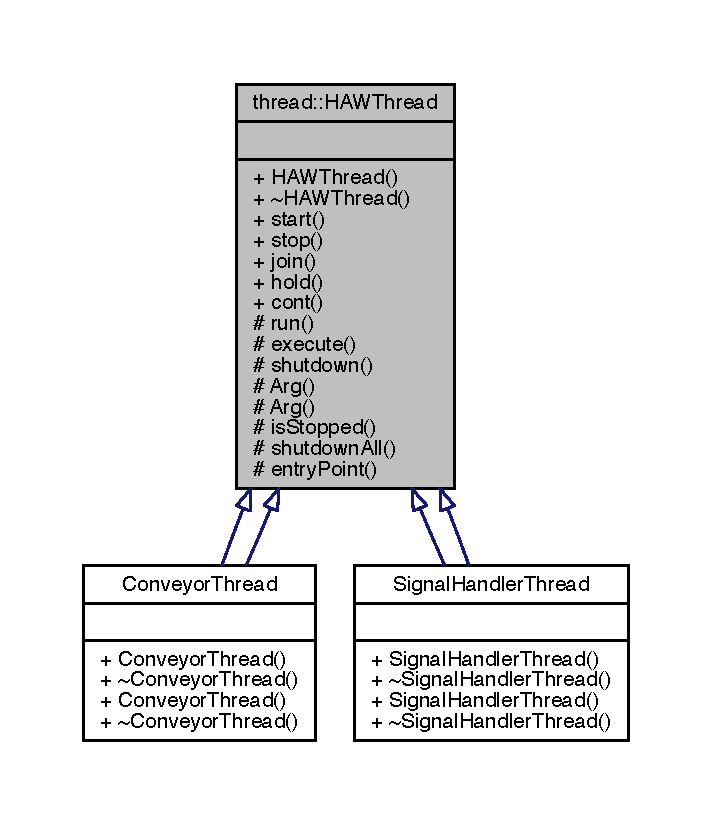
\includegraphics[width=192pt]{classthread_1_1_h_a_w_thread__inherit__graph}
\end{center}
\end{figure}


Zusammengehörigkeiten von thread\+:\+:H\+A\+W\+Thread\+:\nopagebreak
\begin{figure}[H]
\begin{center}
\leavevmode
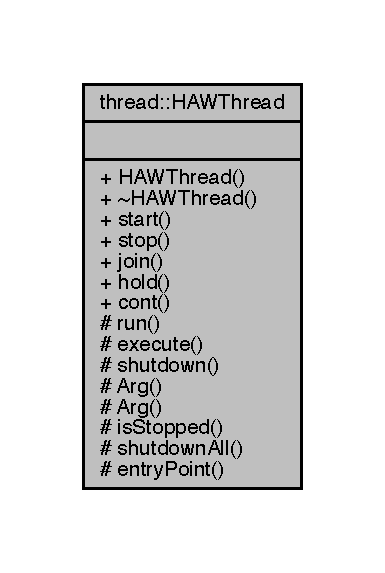
\includegraphics[width=185pt]{classthread_1_1_h_a_w_thread__coll__graph}
\end{center}
\end{figure}
\subsection*{Öffentliche Methoden}
\begin{DoxyCompactItemize}
\item 
\hyperlink{classthread_1_1_h_a_w_thread_a7ae3280c8aee6ae6536c736a20d92e8d}{H\+A\+W\+Thread} ()
\item 
virtual \hyperlink{classthread_1_1_h_a_w_thread_a84706dda23aa384a43ced901381e795b}{$\sim$\+H\+A\+W\+Thread} ()
\item 
virtual void \hyperlink{classthread_1_1_h_a_w_thread_ae08d268c337511a1e67fbbeefcb1e89d}{start} (void $\ast$arg)
\item 
void \hyperlink{classthread_1_1_h_a_w_thread_ae8a89c83fd7e9b9a712c19f636ab2638}{stop} ()
\item 
void \hyperlink{classthread_1_1_h_a_w_thread_adbc0234a7b8eb2271a5cb4a7b8090956}{join} () const
\item 
void \hyperlink{classthread_1_1_h_a_w_thread_a18f2a0cc61833e98b18e56ea541fa38b}{hold} ()
\item 
void \hyperlink{classthread_1_1_h_a_w_thread_a4c480261e3236c90c8de73be55650ba4}{cont} ()
\end{DoxyCompactItemize}
\subsection*{Geschützte Methoden}
\begin{DoxyCompactItemize}
\item 
void \hyperlink{classthread_1_1_h_a_w_thread_a9a3e17be59877d350e310eb19c52679b}{run} (void $\ast$arg)
\item 
virtual void \hyperlink{classthread_1_1_h_a_w_thread_ae565cb73c096b246664bd2474b9c8907}{execute} (void $\ast$)=0
\item 
virtual void \hyperlink{classthread_1_1_h_a_w_thread_a843ee9493a41cec7e932fdec67a3b244}{shutdown} ()=0
\item 
void $\ast$ \hyperlink{classthread_1_1_h_a_w_thread_a87d9850bda803fafa714c32a63c11a89}{Arg} () const
\item 
void \hyperlink{classthread_1_1_h_a_w_thread_a368c07a801fb8f5e7bb181d2453df4be}{Arg} (void $\ast$a)
\item 
bool \hyperlink{classthread_1_1_h_a_w_thread_acd3923a840cbe1fea040fc149c4ab749}{is\+Stopped} () const
\item 
void \hyperlink{classthread_1_1_h_a_w_thread_a5124385e940aa8d52510a4be10af173c}{shutdown\+All} ()
\end{DoxyCompactItemize}
\subsection*{Geschützte, statische Methoden}
\begin{DoxyCompactItemize}
\item 
static void $\ast$ \hyperlink{classthread_1_1_h_a_w_thread_a044da2e1a8884a3e2764f9f1863863c7}{entry\+Point} (void $\ast$)
\end{DoxyCompactItemize}


\subsection{Beschreibung der Konstruktoren und Destruktoren}
\hypertarget{classthread_1_1_h_a_w_thread_a7ae3280c8aee6ae6536c736a20d92e8d}{}\label{classthread_1_1_h_a_w_thread_a7ae3280c8aee6ae6536c736a20d92e8d} 
\index{thread\+::\+H\+A\+W\+Thread@{thread\+::\+H\+A\+W\+Thread}!H\+A\+W\+Thread@{H\+A\+W\+Thread}}
\index{H\+A\+W\+Thread@{H\+A\+W\+Thread}!thread\+::\+H\+A\+W\+Thread@{thread\+::\+H\+A\+W\+Thread}}
\subsubsection{\texorpdfstring{H\+A\+W\+Thread()}{HAWThread()}}
{\footnotesize\ttfamily thread\+::\+H\+A\+W\+Thread\+::\+H\+A\+W\+Thread (\begin{DoxyParamCaption}{ }\end{DoxyParamCaption})}

Constructor. Initializes members \hypertarget{classthread_1_1_h_a_w_thread_a84706dda23aa384a43ced901381e795b}{}\label{classthread_1_1_h_a_w_thread_a84706dda23aa384a43ced901381e795b} 
\index{thread\+::\+H\+A\+W\+Thread@{thread\+::\+H\+A\+W\+Thread}!````~H\+A\+W\+Thread@{$\sim$\+H\+A\+W\+Thread}}
\index{````~H\+A\+W\+Thread@{$\sim$\+H\+A\+W\+Thread}!thread\+::\+H\+A\+W\+Thread@{thread\+::\+H\+A\+W\+Thread}}
\subsubsection{\texorpdfstring{$\sim$\+H\+A\+W\+Thread()}{~HAWThread()}}
{\footnotesize\ttfamily thread\+::\+H\+A\+W\+Thread\+::$\sim$\+H\+A\+W\+Thread (\begin{DoxyParamCaption}{ }\end{DoxyParamCaption})\hspace{0.3cm}{\ttfamily [virtual]}}

Destructor. Calls Thread\+Destroy. This should shutdown the thread more carefully. \begin{DoxyWarning}{Warnung}
needs some work! 
\end{DoxyWarning}


\subsection{Dokumentation der Elementfunktionen}
\hypertarget{classthread_1_1_h_a_w_thread_a87d9850bda803fafa714c32a63c11a89}{}\label{classthread_1_1_h_a_w_thread_a87d9850bda803fafa714c32a63c11a89} 
\index{thread\+::\+H\+A\+W\+Thread@{thread\+::\+H\+A\+W\+Thread}!Arg@{Arg}}
\index{Arg@{Arg}!thread\+::\+H\+A\+W\+Thread@{thread\+::\+H\+A\+W\+Thread}}
\subsubsection{\texorpdfstring{Arg()}{Arg()}\hspace{0.1cm}{\footnotesize\ttfamily [1/2]}}
{\footnotesize\ttfamily void$\ast$ thread\+::\+H\+A\+W\+Thread\+::\+Arg (\begin{DoxyParamCaption}{ }\end{DoxyParamCaption}) const\hspace{0.3cm}{\ttfamily [inline]}, {\ttfamily [protected]}}

used internally to pass the argument. \hypertarget{classthread_1_1_h_a_w_thread_a368c07a801fb8f5e7bb181d2453df4be}{}\label{classthread_1_1_h_a_w_thread_a368c07a801fb8f5e7bb181d2453df4be} 
\index{thread\+::\+H\+A\+W\+Thread@{thread\+::\+H\+A\+W\+Thread}!Arg@{Arg}}
\index{Arg@{Arg}!thread\+::\+H\+A\+W\+Thread@{thread\+::\+H\+A\+W\+Thread}}
\subsubsection{\texorpdfstring{Arg()}{Arg()}\hspace{0.1cm}{\footnotesize\ttfamily [2/2]}}
{\footnotesize\ttfamily void thread\+::\+H\+A\+W\+Thread\+::\+Arg (\begin{DoxyParamCaption}\item[{void $\ast$}]{a }\end{DoxyParamCaption})\hspace{0.3cm}{\ttfamily [inline]}, {\ttfamily [protected]}}

used internally to set the arguement. \hypertarget{classthread_1_1_h_a_w_thread_a4c480261e3236c90c8de73be55650ba4}{}\label{classthread_1_1_h_a_w_thread_a4c480261e3236c90c8de73be55650ba4} 
\index{thread\+::\+H\+A\+W\+Thread@{thread\+::\+H\+A\+W\+Thread}!cont@{cont}}
\index{cont@{cont}!thread\+::\+H\+A\+W\+Thread@{thread\+::\+H\+A\+W\+Thread}}
\subsubsection{\texorpdfstring{cont()}{cont()}}
{\footnotesize\ttfamily void thread\+::\+H\+A\+W\+Thread\+::cont (\begin{DoxyParamCaption}{ }\end{DoxyParamCaption})}

This function continues (resumes) the thread. It makes a Thread\+Ctrl call. \hypertarget{classthread_1_1_h_a_w_thread_a044da2e1a8884a3e2764f9f1863863c7}{}\label{classthread_1_1_h_a_w_thread_a044da2e1a8884a3e2764f9f1863863c7} 
\index{thread\+::\+H\+A\+W\+Thread@{thread\+::\+H\+A\+W\+Thread}!entry\+Point@{entry\+Point}}
\index{entry\+Point@{entry\+Point}!thread\+::\+H\+A\+W\+Thread@{thread\+::\+H\+A\+W\+Thread}}
\subsubsection{\texorpdfstring{entry\+Point()}{entryPoint()}}
{\footnotesize\ttfamily void $\ast$ thread\+::\+H\+A\+W\+Thread\+::entry\+Point (\begin{DoxyParamCaption}\item[{void $\ast$}]{pthis }\end{DoxyParamCaption})\hspace{0.3cm}{\ttfamily [static]}, {\ttfamily [protected]}}

\hypertarget{classthread_1_1_h_a_w_thread_ae565cb73c096b246664bd2474b9c8907}{}\label{classthread_1_1_h_a_w_thread_ae565cb73c096b246664bd2474b9c8907} 
\index{thread\+::\+H\+A\+W\+Thread@{thread\+::\+H\+A\+W\+Thread}!execute@{execute}}
\index{execute@{execute}!thread\+::\+H\+A\+W\+Thread@{thread\+::\+H\+A\+W\+Thread}}
\subsubsection{\texorpdfstring{execute()}{execute()}}
{\footnotesize\ttfamily virtual void thread\+::\+H\+A\+W\+Thread\+::execute (\begin{DoxyParamCaption}\item[{void $\ast$}]{ }\end{DoxyParamCaption})\hspace{0.3cm}{\ttfamily [protected]}, {\ttfamily [pure virtual]}}

to be implemented in the derived class. The application programmer has to write his own loop. He can check bool \hyperlink{classthread_1_1_h_a_w_thread_acd3923a840cbe1fea040fc149c4ab749}{is\+Stopped()} to see if the thread should exit the loop. \hypertarget{classthread_1_1_h_a_w_thread_a18f2a0cc61833e98b18e56ea541fa38b}{}\label{classthread_1_1_h_a_w_thread_a18f2a0cc61833e98b18e56ea541fa38b} 
\index{thread\+::\+H\+A\+W\+Thread@{thread\+::\+H\+A\+W\+Thread}!hold@{hold}}
\index{hold@{hold}!thread\+::\+H\+A\+W\+Thread@{thread\+::\+H\+A\+W\+Thread}}
\subsubsection{\texorpdfstring{hold()}{hold()}}
{\footnotesize\ttfamily void thread\+::\+H\+A\+W\+Thread\+::hold (\begin{DoxyParamCaption}{ }\end{DoxyParamCaption})}

This function holds (suspends) the thread. It makes a Thread\+Ctrl call. It shall be used if the thread is not being used for a while but may be used later \hypertarget{classthread_1_1_h_a_w_thread_acd3923a840cbe1fea040fc149c4ab749}{}\label{classthread_1_1_h_a_w_thread_acd3923a840cbe1fea040fc149c4ab749} 
\index{thread\+::\+H\+A\+W\+Thread@{thread\+::\+H\+A\+W\+Thread}!is\+Stopped@{is\+Stopped}}
\index{is\+Stopped@{is\+Stopped}!thread\+::\+H\+A\+W\+Thread@{thread\+::\+H\+A\+W\+Thread}}
\subsubsection{\texorpdfstring{is\+Stopped()}{isStopped()}}
{\footnotesize\ttfamily bool thread\+::\+H\+A\+W\+Thread\+::is\+Stopped (\begin{DoxyParamCaption}{ }\end{DoxyParamCaption}) const\hspace{0.3cm}{\ttfamily [inline]}, {\ttfamily [protected]}}

returns the stop-\/status of the thread. This function should be checked by the user function execute regularly. \hypertarget{classthread_1_1_h_a_w_thread_adbc0234a7b8eb2271a5cb4a7b8090956}{}\label{classthread_1_1_h_a_w_thread_adbc0234a7b8eb2271a5cb4a7b8090956} 
\index{thread\+::\+H\+A\+W\+Thread@{thread\+::\+H\+A\+W\+Thread}!join@{join}}
\index{join@{join}!thread\+::\+H\+A\+W\+Thread@{thread\+::\+H\+A\+W\+Thread}}
\subsubsection{\texorpdfstring{join()}{join()}}
{\footnotesize\ttfamily void thread\+::\+H\+A\+W\+Thread\+::join (\begin{DoxyParamCaption}{ }\end{DoxyParamCaption}) const}

Calls join on the thread. \begin{DoxyWarning}{Warnung}
must be called from the same context as start. 
\end{DoxyWarning}
\hypertarget{classthread_1_1_h_a_w_thread_a9a3e17be59877d350e310eb19c52679b}{}\label{classthread_1_1_h_a_w_thread_a9a3e17be59877d350e310eb19c52679b} 
\index{thread\+::\+H\+A\+W\+Thread@{thread\+::\+H\+A\+W\+Thread}!run@{run}}
\index{run@{run}!thread\+::\+H\+A\+W\+Thread@{thread\+::\+H\+A\+W\+Thread}}
\subsubsection{\texorpdfstring{run()}{run()}}
{\footnotesize\ttfamily void thread\+::\+H\+A\+W\+Thread\+::run (\begin{DoxyParamCaption}\item[{void $\ast$}]{arg }\end{DoxyParamCaption})\hspace{0.3cm}{\ttfamily [protected]}}

This is called when the thread is started. It calls execute an shutdown which are the user functions. \hypertarget{classthread_1_1_h_a_w_thread_a843ee9493a41cec7e932fdec67a3b244}{}\label{classthread_1_1_h_a_w_thread_a843ee9493a41cec7e932fdec67a3b244} 
\index{thread\+::\+H\+A\+W\+Thread@{thread\+::\+H\+A\+W\+Thread}!shutdown@{shutdown}}
\index{shutdown@{shutdown}!thread\+::\+H\+A\+W\+Thread@{thread\+::\+H\+A\+W\+Thread}}
\subsubsection{\texorpdfstring{shutdown()}{shutdown()}}
{\footnotesize\ttfamily virtual void thread\+::\+H\+A\+W\+Thread\+::shutdown (\begin{DoxyParamCaption}{ }\end{DoxyParamCaption})\hspace{0.3cm}{\ttfamily [protected]}, {\ttfamily [pure virtual]}}

this function must be implemented in the derived class. The function is called once after the thread has been stopped. \hypertarget{classthread_1_1_h_a_w_thread_a5124385e940aa8d52510a4be10af173c}{}\label{classthread_1_1_h_a_w_thread_a5124385e940aa8d52510a4be10af173c} 
\index{thread\+::\+H\+A\+W\+Thread@{thread\+::\+H\+A\+W\+Thread}!shutdown\+All@{shutdown\+All}}
\index{shutdown\+All@{shutdown\+All}!thread\+::\+H\+A\+W\+Thread@{thread\+::\+H\+A\+W\+Thread}}
\subsubsection{\texorpdfstring{shutdown\+All()}{shutdownAll()}}
{\footnotesize\ttfamily void thread\+::\+H\+A\+W\+Thread\+::shutdown\+All (\begin{DoxyParamCaption}{ }\end{DoxyParamCaption})\hspace{0.3cm}{\ttfamily [inline]}, {\ttfamily [protected]}}

sets the G\+L\+O\+B\+A\+L\+\_\+\+E\+X\+IT flag to true. \hypertarget{classthread_1_1_h_a_w_thread_ae08d268c337511a1e67fbbeefcb1e89d}{}\label{classthread_1_1_h_a_w_thread_ae08d268c337511a1e67fbbeefcb1e89d} 
\index{thread\+::\+H\+A\+W\+Thread@{thread\+::\+H\+A\+W\+Thread}!start@{start}}
\index{start@{start}!thread\+::\+H\+A\+W\+Thread@{thread\+::\+H\+A\+W\+Thread}}
\subsubsection{\texorpdfstring{start()}{start()}}
{\footnotesize\ttfamily void thread\+::\+H\+A\+W\+Thread\+::start (\begin{DoxyParamCaption}\item[{void $\ast$}]{arg }\end{DoxyParamCaption})\hspace{0.3cm}{\ttfamily [virtual]}}

Starts the Thread. \begin{DoxyWarning}{Warnung}
start must be called always from the same context as \hyperlink{classthread_1_1_h_a_w_thread_ae8a89c83fd7e9b9a712c19f636ab2638}{stop()}. 

If Thread is already running, \hyperlink{classthread_1_1_h_a_w_thread_ae08d268c337511a1e67fbbeefcb1e89d}{start()} is a N\+OP. \begin{DoxyItemize}
\item argument is stored locally as a member. \end{DoxyItemize}

\end{DoxyWarning}
\hypertarget{classthread_1_1_h_a_w_thread_ae8a89c83fd7e9b9a712c19f636ab2638}{}\label{classthread_1_1_h_a_w_thread_ae8a89c83fd7e9b9a712c19f636ab2638} 
\index{thread\+::\+H\+A\+W\+Thread@{thread\+::\+H\+A\+W\+Thread}!stop@{stop}}
\index{stop@{stop}!thread\+::\+H\+A\+W\+Thread@{thread\+::\+H\+A\+W\+Thread}}
\subsubsection{\texorpdfstring{stop()}{stop()}}
{\footnotesize\ttfamily void thread\+::\+H\+A\+W\+Thread\+::stop (\begin{DoxyParamCaption}{ }\end{DoxyParamCaption})}

Sets the internal flag L\+O\+C\+A\+L\+\_\+\+E\+X\+IT to true. 

Die Dokumentation für diese Klasse wurde erzeugt aufgrund der Dateien\+:\begin{DoxyCompactItemize}
\item 
src/lib/\hyperlink{_h_a_w_thread_8h}{H\+A\+W\+Thread.\+h}\item 
src/lib/\hyperlink{_h_a_w_thread_8cpp}{H\+A\+W\+Thread.\+cpp}\end{DoxyCompactItemize}

\hypertarget{class_human_machine_interface}{}\section{Human\+Machine\+Interface Klassenreferenz}
\label{class_human_machine_interface}\index{Human\+Machine\+Interface@{Human\+Machine\+Interface}}


{\ttfamily \#include $<$Human\+Machine\+Interface.\+h$>$}



Zusammengehörigkeiten von Human\+Machine\+Interface\+:\nopagebreak
\begin{figure}[H]
\begin{center}
\leavevmode
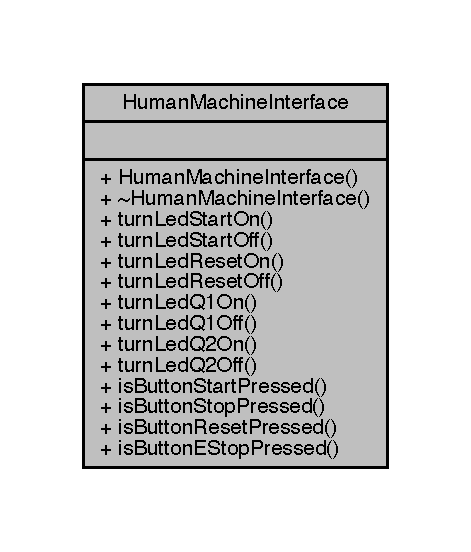
\includegraphics[width=226pt]{class_human_machine_interface__coll__graph}
\end{center}
\end{figure}
\subsection*{Öffentliche Methoden}
\begin{DoxyCompactItemize}
\item 
\hyperlink{class_human_machine_interface_aee37229a726c66857601422ba1605ac6}{Human\+Machine\+Interface} (\hyperlink{class_adapter}{Adapter} $\ast$adapt)
\item 
virtual \hyperlink{class_human_machine_interface_a2ac7ae9e7e6be379da946eac459ea243}{$\sim$\+Human\+Machine\+Interface} ()
\item 
uint8\+\_\+t \hyperlink{class_human_machine_interface_a46dca7b3435dc4b20a2db67b301cb36d}{turn\+Led\+Start\+On} ()
\item 
uint8\+\_\+t \hyperlink{class_human_machine_interface_a235557e9ae72f14a4db72bab675eaae1}{turn\+Led\+Start\+Off} ()
\item 
uint8\+\_\+t \hyperlink{class_human_machine_interface_aecc34d7d1e3edbe2ed38e3808da65455}{turn\+Led\+Reset\+On} ()
\item 
uint8\+\_\+t \hyperlink{class_human_machine_interface_a446ad469f8c9f2717d12cc69ea68598f}{turn\+Led\+Reset\+Off} ()
\item 
uint8\+\_\+t \hyperlink{class_human_machine_interface_a0ba867b5493f024f53c1e00a1287aa6c}{turn\+Led\+Q1\+On} ()
\item 
uint8\+\_\+t \hyperlink{class_human_machine_interface_a7d696c1803928a001bb98585f2ceb138}{turn\+Led\+Q1\+Off} ()
\item 
uint8\+\_\+t \hyperlink{class_human_machine_interface_a9fcfd97db711e6954cbfeec8f93efb58}{turn\+Led\+Q2\+On} ()
\item 
uint8\+\_\+t \hyperlink{class_human_machine_interface_a73d76c6dd54b115fa8df9cf5f2b0d2aa}{turn\+Led\+Q2\+Off} ()
\item 
uint8\+\_\+t \hyperlink{class_human_machine_interface_a4926796f1c1411f975e2da96c68079dd}{is\+Button\+Start\+Pressed} ()
\item 
uint8\+\_\+t \hyperlink{class_human_machine_interface_a6b150a5a2978b620a3823aaeda7e80b8}{is\+Button\+Stop\+Pressed} ()
\item 
uint8\+\_\+t \hyperlink{class_human_machine_interface_ab78f8bd8db3e0b150699416d8081ee98}{is\+Button\+Reset\+Pressed} ()
\item 
uint8\+\_\+t \hyperlink{class_human_machine_interface_ad9844e21fd01872ad78afb9e16acc59f}{is\+Button\+E\+Stop\+Pressed} ()
\end{DoxyCompactItemize}


\subsection{Beschreibung der Konstruktoren und Destruktoren}
\hypertarget{class_human_machine_interface_aee37229a726c66857601422ba1605ac6}{}\label{class_human_machine_interface_aee37229a726c66857601422ba1605ac6} 
\index{Human\+Machine\+Interface@{Human\+Machine\+Interface}!Human\+Machine\+Interface@{Human\+Machine\+Interface}}
\index{Human\+Machine\+Interface@{Human\+Machine\+Interface}!Human\+Machine\+Interface@{Human\+Machine\+Interface}}
\subsubsection{\texorpdfstring{Human\+Machine\+Interface()}{HumanMachineInterface()}}
{\footnotesize\ttfamily Human\+Machine\+Interface\+::\+Human\+Machine\+Interface (\begin{DoxyParamCaption}\item[{\hyperlink{class_adapter}{Adapter} $\ast$}]{adapt }\end{DoxyParamCaption})}

Constructor des \hyperlink{class_human_machine_interface}{Human\+Machine\+Interface} \hypertarget{class_human_machine_interface_a2ac7ae9e7e6be379da946eac459ea243}{}\label{class_human_machine_interface_a2ac7ae9e7e6be379da946eac459ea243} 
\index{Human\+Machine\+Interface@{Human\+Machine\+Interface}!````~Human\+Machine\+Interface@{$\sim$\+Human\+Machine\+Interface}}
\index{````~Human\+Machine\+Interface@{$\sim$\+Human\+Machine\+Interface}!Human\+Machine\+Interface@{Human\+Machine\+Interface}}
\subsubsection{\texorpdfstring{$\sim$\+Human\+Machine\+Interface()}{~HumanMachineInterface()}}
{\footnotesize\ttfamily Human\+Machine\+Interface\+::$\sim$\+Human\+Machine\+Interface (\begin{DoxyParamCaption}{ }\end{DoxyParamCaption})\hspace{0.3cm}{\ttfamily [virtual]}}

Constructor des \hyperlink{class_human_machine_interface}{Human\+Machine\+Interface} 

\subsection{Dokumentation der Elementfunktionen}
\hypertarget{class_human_machine_interface_ad9844e21fd01872ad78afb9e16acc59f}{}\label{class_human_machine_interface_ad9844e21fd01872ad78afb9e16acc59f} 
\index{Human\+Machine\+Interface@{Human\+Machine\+Interface}!is\+Button\+E\+Stop\+Pressed@{is\+Button\+E\+Stop\+Pressed}}
\index{is\+Button\+E\+Stop\+Pressed@{is\+Button\+E\+Stop\+Pressed}!Human\+Machine\+Interface@{Human\+Machine\+Interface}}
\subsubsection{\texorpdfstring{is\+Button\+E\+Stop\+Pressed()}{isButtonEStopPressed()}}
{\footnotesize\ttfamily uint8\+\_\+t Human\+Machine\+Interface\+::is\+Button\+E\+Stop\+Pressed (\begin{DoxyParamCaption}{ }\end{DoxyParamCaption})}

Checkt ob der Button E\+Stop gedrueckt wird.

\begin{DoxyReturn}{Rückgabe}
Gibt 0 zurueck bei F\+A\+L\+SE ansonsten ein Wert $>$0. 
\end{DoxyReturn}
\hypertarget{class_human_machine_interface_ab78f8bd8db3e0b150699416d8081ee98}{}\label{class_human_machine_interface_ab78f8bd8db3e0b150699416d8081ee98} 
\index{Human\+Machine\+Interface@{Human\+Machine\+Interface}!is\+Button\+Reset\+Pressed@{is\+Button\+Reset\+Pressed}}
\index{is\+Button\+Reset\+Pressed@{is\+Button\+Reset\+Pressed}!Human\+Machine\+Interface@{Human\+Machine\+Interface}}
\subsubsection{\texorpdfstring{is\+Button\+Reset\+Pressed()}{isButtonResetPressed()}}
{\footnotesize\ttfamily uint8\+\_\+t Human\+Machine\+Interface\+::is\+Button\+Reset\+Pressed (\begin{DoxyParamCaption}{ }\end{DoxyParamCaption})}

Checkt ob der Button Reset gedrueckt wird.

\begin{DoxyReturn}{Rückgabe}
Gibt 0 zurueck bei F\+A\+L\+SE ansonsten ein Wert $>$0. 
\end{DoxyReturn}
\hypertarget{class_human_machine_interface_a4926796f1c1411f975e2da96c68079dd}{}\label{class_human_machine_interface_a4926796f1c1411f975e2da96c68079dd} 
\index{Human\+Machine\+Interface@{Human\+Machine\+Interface}!is\+Button\+Start\+Pressed@{is\+Button\+Start\+Pressed}}
\index{is\+Button\+Start\+Pressed@{is\+Button\+Start\+Pressed}!Human\+Machine\+Interface@{Human\+Machine\+Interface}}
\subsubsection{\texorpdfstring{is\+Button\+Start\+Pressed()}{isButtonStartPressed()}}
{\footnotesize\ttfamily uint8\+\_\+t Human\+Machine\+Interface\+::is\+Button\+Start\+Pressed (\begin{DoxyParamCaption}{ }\end{DoxyParamCaption})}

Checkt ob der Button Start gedrueckt wird.

\begin{DoxyReturn}{Rückgabe}
Gibt 0 zurueck bei F\+A\+L\+SE ansonsten ein Wert $>$0. 
\end{DoxyReturn}
\hypertarget{class_human_machine_interface_a6b150a5a2978b620a3823aaeda7e80b8}{}\label{class_human_machine_interface_a6b150a5a2978b620a3823aaeda7e80b8} 
\index{Human\+Machine\+Interface@{Human\+Machine\+Interface}!is\+Button\+Stop\+Pressed@{is\+Button\+Stop\+Pressed}}
\index{is\+Button\+Stop\+Pressed@{is\+Button\+Stop\+Pressed}!Human\+Machine\+Interface@{Human\+Machine\+Interface}}
\subsubsection{\texorpdfstring{is\+Button\+Stop\+Pressed()}{isButtonStopPressed()}}
{\footnotesize\ttfamily uint8\+\_\+t Human\+Machine\+Interface\+::is\+Button\+Stop\+Pressed (\begin{DoxyParamCaption}{ }\end{DoxyParamCaption})}

Checkt ob der Button Stop gedrueckt wird.

\begin{DoxyReturn}{Rückgabe}
Gibt 0 zurueck bei F\+A\+L\+SE ansonsten ein Wert $>$0. 
\end{DoxyReturn}
\hypertarget{class_human_machine_interface_a7d696c1803928a001bb98585f2ceb138}{}\label{class_human_machine_interface_a7d696c1803928a001bb98585f2ceb138} 
\index{Human\+Machine\+Interface@{Human\+Machine\+Interface}!turn\+Led\+Q1\+Off@{turn\+Led\+Q1\+Off}}
\index{turn\+Led\+Q1\+Off@{turn\+Led\+Q1\+Off}!Human\+Machine\+Interface@{Human\+Machine\+Interface}}
\subsubsection{\texorpdfstring{turn\+Led\+Q1\+Off()}{turnLedQ1Off()}}
{\footnotesize\ttfamily uint8\+\_\+t Human\+Machine\+Interface\+::turn\+Led\+Q1\+Off (\begin{DoxyParamCaption}{ }\end{DoxyParamCaption})}

Macht die Lampe Q1 aus.

\begin{DoxyReturn}{Rückgabe}
Gibt Konstant 0 zurueck. 
\end{DoxyReturn}
\hypertarget{class_human_machine_interface_a0ba867b5493f024f53c1e00a1287aa6c}{}\label{class_human_machine_interface_a0ba867b5493f024f53c1e00a1287aa6c} 
\index{Human\+Machine\+Interface@{Human\+Machine\+Interface}!turn\+Led\+Q1\+On@{turn\+Led\+Q1\+On}}
\index{turn\+Led\+Q1\+On@{turn\+Led\+Q1\+On}!Human\+Machine\+Interface@{Human\+Machine\+Interface}}
\subsubsection{\texorpdfstring{turn\+Led\+Q1\+On()}{turnLedQ1On()}}
{\footnotesize\ttfamily uint8\+\_\+t Human\+Machine\+Interface\+::turn\+Led\+Q1\+On (\begin{DoxyParamCaption}{ }\end{DoxyParamCaption})}

Macht die Lampe Q1 an.

\begin{DoxyReturn}{Rückgabe}
Gibt Konstant 0 zurueck. 
\end{DoxyReturn}
\hypertarget{class_human_machine_interface_a73d76c6dd54b115fa8df9cf5f2b0d2aa}{}\label{class_human_machine_interface_a73d76c6dd54b115fa8df9cf5f2b0d2aa} 
\index{Human\+Machine\+Interface@{Human\+Machine\+Interface}!turn\+Led\+Q2\+Off@{turn\+Led\+Q2\+Off}}
\index{turn\+Led\+Q2\+Off@{turn\+Led\+Q2\+Off}!Human\+Machine\+Interface@{Human\+Machine\+Interface}}
\subsubsection{\texorpdfstring{turn\+Led\+Q2\+Off()}{turnLedQ2Off()}}
{\footnotesize\ttfamily uint8\+\_\+t Human\+Machine\+Interface\+::turn\+Led\+Q2\+Off (\begin{DoxyParamCaption}{ }\end{DoxyParamCaption})}

Macht die Lampe Q1 aus.

\begin{DoxyReturn}{Rückgabe}
Gibt Konstant 0 zurueck. 
\end{DoxyReturn}
\hypertarget{class_human_machine_interface_a9fcfd97db711e6954cbfeec8f93efb58}{}\label{class_human_machine_interface_a9fcfd97db711e6954cbfeec8f93efb58} 
\index{Human\+Machine\+Interface@{Human\+Machine\+Interface}!turn\+Led\+Q2\+On@{turn\+Led\+Q2\+On}}
\index{turn\+Led\+Q2\+On@{turn\+Led\+Q2\+On}!Human\+Machine\+Interface@{Human\+Machine\+Interface}}
\subsubsection{\texorpdfstring{turn\+Led\+Q2\+On()}{turnLedQ2On()}}
{\footnotesize\ttfamily uint8\+\_\+t Human\+Machine\+Interface\+::turn\+Led\+Q2\+On (\begin{DoxyParamCaption}{ }\end{DoxyParamCaption})}

Macht die Lampe Q2 an.

\begin{DoxyReturn}{Rückgabe}
Gibt Konstant 0 zurueck. 
\end{DoxyReturn}
\hypertarget{class_human_machine_interface_a446ad469f8c9f2717d12cc69ea68598f}{}\label{class_human_machine_interface_a446ad469f8c9f2717d12cc69ea68598f} 
\index{Human\+Machine\+Interface@{Human\+Machine\+Interface}!turn\+Led\+Reset\+Off@{turn\+Led\+Reset\+Off}}
\index{turn\+Led\+Reset\+Off@{turn\+Led\+Reset\+Off}!Human\+Machine\+Interface@{Human\+Machine\+Interface}}
\subsubsection{\texorpdfstring{turn\+Led\+Reset\+Off()}{turnLedResetOff()}}
{\footnotesize\ttfamily uint8\+\_\+t Human\+Machine\+Interface\+::turn\+Led\+Reset\+Off (\begin{DoxyParamCaption}{ }\end{DoxyParamCaption})}

Macht die Lampe auf dem Reset Button aus.

\begin{DoxyReturn}{Rückgabe}
Gibt Konstant 0 zurueck. 
\end{DoxyReturn}
\hypertarget{class_human_machine_interface_aecc34d7d1e3edbe2ed38e3808da65455}{}\label{class_human_machine_interface_aecc34d7d1e3edbe2ed38e3808da65455} 
\index{Human\+Machine\+Interface@{Human\+Machine\+Interface}!turn\+Led\+Reset\+On@{turn\+Led\+Reset\+On}}
\index{turn\+Led\+Reset\+On@{turn\+Led\+Reset\+On}!Human\+Machine\+Interface@{Human\+Machine\+Interface}}
\subsubsection{\texorpdfstring{turn\+Led\+Reset\+On()}{turnLedResetOn()}}
{\footnotesize\ttfamily uint8\+\_\+t Human\+Machine\+Interface\+::turn\+Led\+Reset\+On (\begin{DoxyParamCaption}{ }\end{DoxyParamCaption})}

Macht die Lampe auf dem Reset Button an.

\begin{DoxyReturn}{Rückgabe}
Gibt Konstant 0 zurueck. 
\end{DoxyReturn}
\hypertarget{class_human_machine_interface_a235557e9ae72f14a4db72bab675eaae1}{}\label{class_human_machine_interface_a235557e9ae72f14a4db72bab675eaae1} 
\index{Human\+Machine\+Interface@{Human\+Machine\+Interface}!turn\+Led\+Start\+Off@{turn\+Led\+Start\+Off}}
\index{turn\+Led\+Start\+Off@{turn\+Led\+Start\+Off}!Human\+Machine\+Interface@{Human\+Machine\+Interface}}
\subsubsection{\texorpdfstring{turn\+Led\+Start\+Off()}{turnLedStartOff()}}
{\footnotesize\ttfamily uint8\+\_\+t Human\+Machine\+Interface\+::turn\+Led\+Start\+Off (\begin{DoxyParamCaption}{ }\end{DoxyParamCaption})}

Macht die Lampe auf dem Start Button aus.

\begin{DoxyReturn}{Rückgabe}
Gibt Konstant 0 zurueck. 
\end{DoxyReturn}
\hypertarget{class_human_machine_interface_a46dca7b3435dc4b20a2db67b301cb36d}{}\label{class_human_machine_interface_a46dca7b3435dc4b20a2db67b301cb36d} 
\index{Human\+Machine\+Interface@{Human\+Machine\+Interface}!turn\+Led\+Start\+On@{turn\+Led\+Start\+On}}
\index{turn\+Led\+Start\+On@{turn\+Led\+Start\+On}!Human\+Machine\+Interface@{Human\+Machine\+Interface}}
\subsubsection{\texorpdfstring{turn\+Led\+Start\+On()}{turnLedStartOn()}}
{\footnotesize\ttfamily uint8\+\_\+t Human\+Machine\+Interface\+::turn\+Led\+Start\+On (\begin{DoxyParamCaption}{ }\end{DoxyParamCaption})}

Macht die Lampe auf dem Start Button an.

\begin{DoxyReturn}{Rückgabe}
Gibt Konstant 0 zurueck. 
\end{DoxyReturn}


Die Dokumentation für diese Klasse wurde erzeugt aufgrund der Dateien\+:\begin{DoxyCompactItemize}
\item 
Hal/\hyperlink{_human_machine_interface_8h}{Human\+Machine\+Interface.\+h}\item 
Hal/\hyperlink{_human_machine_interface_8cpp}{Human\+Machine\+Interface.\+cpp}\end{DoxyCompactItemize}

\hypertarget{class_logger}{}\section{Logger Klassenreferenz}
\label{class_logger}\index{Logger@{Logger}}


{\ttfamily \#include $<$Logger.\+h$>$}



Zusammengehörigkeiten von Logger\+:\nopagebreak
\begin{figure}[H]
\begin{center}
\leavevmode
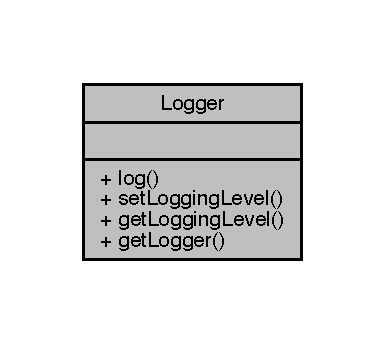
\includegraphics[width=185pt]{class_logger__coll__graph}
\end{center}
\end{figure}
\subsection*{Öffentliche Methoden}
\begin{DoxyCompactItemize}
\item 
std\+::ofstream \& \hyperlink{class_logger_af8a0b7a8939294ceb2cef39c358dfa9c}{log} ()
\item 
void \hyperlink{class_logger_a3759fa32a4f0c7255f61a2ce6484c194}{set\+Logging\+Level} (\hyperlink{_logger_8h_aa5a9053636a30269210c54e734e0d583}{L\+O\+G\+\_\+\+L\+E\+V\+EL} level)
\item 
\hyperlink{_logger_8h_aa5a9053636a30269210c54e734e0d583}{L\+O\+G\+\_\+\+L\+E\+V\+EL} \hyperlink{class_logger_acce532a939622d2b5c919f5f67236564}{get\+Logging\+Level} ()
\end{DoxyCompactItemize}
\subsection*{Öffentliche, statische Methoden}
\begin{DoxyCompactItemize}
\item 
static \hyperlink{class_logger}{Logger} \& \hyperlink{class_logger_afa2765f0a04e7a50e1efc38cce67a763}{get\+Logger} ()
\end{DoxyCompactItemize}


\subsection{Dokumentation der Elementfunktionen}
\hypertarget{class_logger_afa2765f0a04e7a50e1efc38cce67a763}{}\label{class_logger_afa2765f0a04e7a50e1efc38cce67a763} 
\index{Logger@{Logger}!get\+Logger@{get\+Logger}}
\index{get\+Logger@{get\+Logger}!Logger@{Logger}}
\subsubsection{\texorpdfstring{get\+Logger()}{getLogger()}}
{\footnotesize\ttfamily static \hyperlink{class_logger}{Logger}\& Logger\+::get\+Logger (\begin{DoxyParamCaption}{ }\end{DoxyParamCaption})\hspace{0.3cm}{\ttfamily [inline]}, {\ttfamily [static]}}

\hypertarget{class_logger_acce532a939622d2b5c919f5f67236564}{}\label{class_logger_acce532a939622d2b5c919f5f67236564} 
\index{Logger@{Logger}!get\+Logging\+Level@{get\+Logging\+Level}}
\index{get\+Logging\+Level@{get\+Logging\+Level}!Logger@{Logger}}
\subsubsection{\texorpdfstring{get\+Logging\+Level()}{getLoggingLevel()}}
{\footnotesize\ttfamily \hyperlink{_logger_8h_aa5a9053636a30269210c54e734e0d583}{L\+O\+G\+\_\+\+L\+E\+V\+EL} Logger\+::get\+Logging\+Level (\begin{DoxyParamCaption}{ }\end{DoxyParamCaption})}

\hypertarget{class_logger_af8a0b7a8939294ceb2cef39c358dfa9c}{}\label{class_logger_af8a0b7a8939294ceb2cef39c358dfa9c} 
\index{Logger@{Logger}!log@{log}}
\index{log@{log}!Logger@{Logger}}
\subsubsection{\texorpdfstring{log()}{log()}}
{\footnotesize\ttfamily std\+::ofstream \& Logger\+::log (\begin{DoxyParamCaption}{ }\end{DoxyParamCaption})}

\hypertarget{class_logger_a3759fa32a4f0c7255f61a2ce6484c194}{}\label{class_logger_a3759fa32a4f0c7255f61a2ce6484c194} 
\index{Logger@{Logger}!set\+Logging\+Level@{set\+Logging\+Level}}
\index{set\+Logging\+Level@{set\+Logging\+Level}!Logger@{Logger}}
\subsubsection{\texorpdfstring{set\+Logging\+Level()}{setLoggingLevel()}}
{\footnotesize\ttfamily void Logger\+::set\+Logging\+Level (\begin{DoxyParamCaption}\item[{\hyperlink{_logger_8h_aa5a9053636a30269210c54e734e0d583}{L\+O\+G\+\_\+\+L\+E\+V\+EL}}]{level }\end{DoxyParamCaption})}



Die Dokumentation für diese Klasse wurde erzeugt aufgrund der Dateien\+:\begin{DoxyCompactItemize}
\item 
Logger/\hyperlink{_logger_8h}{Logger.\+h}\item 
Logger/\hyperlink{_logger_8cpp}{Logger.\+cpp}\end{DoxyCompactItemize}

\hypertarget{class_measuring_tool}{}\section{Measuring\+Tool Klassenreferenz}
\label{class_measuring_tool}\index{Measuring\+Tool@{Measuring\+Tool}}


{\ttfamily \#include $<$Measuring\+Tool.\+h$>$}



Zusammengehörigkeiten von Measuring\+Tool\+:\nopagebreak
\begin{figure}[H]
\begin{center}
\leavevmode
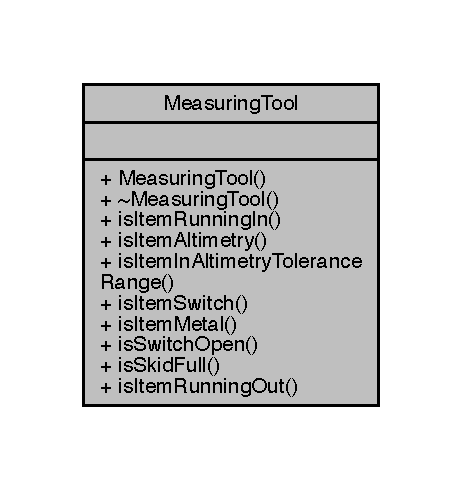
\includegraphics[width=222pt]{class_measuring_tool__coll__graph}
\end{center}
\end{figure}
\subsection*{Öffentliche Methoden}
\begin{DoxyCompactItemize}
\item 
\hyperlink{class_measuring_tool_a2528d2728f77b7f2ed61a9f364340bb8}{Measuring\+Tool} (\hyperlink{class_adapter}{Adapter} $\ast$adapt)
\item 
virtual \hyperlink{class_measuring_tool_a35667285cd41bda48fcc747194c862cd}{$\sim$\+Measuring\+Tool} ()
\item 
uint8\+\_\+t \hyperlink{class_measuring_tool_a1749a84c95ae88ef6e8e65edfa2204bc}{is\+Item\+Running\+In} ()
\item 
uint8\+\_\+t \hyperlink{class_measuring_tool_aebbb332d935cadef3c072ca7102896d3}{is\+Item\+Altimetry} ()
\item 
uint8\+\_\+t \hyperlink{class_measuring_tool_a431263df5654d0dc1587ef23e97c1392}{is\+Item\+In\+Altimetry\+Tolerance\+Range} ()
\item 
uint8\+\_\+t \hyperlink{class_measuring_tool_a25d27399efb7e1a0daceeb270e9c26cc}{is\+Item\+Switch} ()
\item 
uint8\+\_\+t \hyperlink{class_measuring_tool_a1d98ab82733fbdee6e63f880a8ace322}{is\+Item\+Metal} ()
\item 
uint8\+\_\+t \hyperlink{class_measuring_tool_ad46b12c36f63fa9b597b1df6468d6aac}{is\+Switch\+Open} ()
\item 
uint8\+\_\+t \hyperlink{class_measuring_tool_a33ece6093e5b77f9353f86d2d9be64f6}{is\+Skid\+Full} ()
\item 
uint8\+\_\+t \hyperlink{class_measuring_tool_a0941de19234c2026359e4cc973f7bb1b}{is\+Item\+Running\+Out} ()
\end{DoxyCompactItemize}


\subsection{Beschreibung der Konstruktoren und Destruktoren}
\hypertarget{class_measuring_tool_a2528d2728f77b7f2ed61a9f364340bb8}{}\label{class_measuring_tool_a2528d2728f77b7f2ed61a9f364340bb8} 
\index{Measuring\+Tool@{Measuring\+Tool}!Measuring\+Tool@{Measuring\+Tool}}
\index{Measuring\+Tool@{Measuring\+Tool}!Measuring\+Tool@{Measuring\+Tool}}
\subsubsection{\texorpdfstring{Measuring\+Tool()}{MeasuringTool()}}
{\footnotesize\ttfamily Measuring\+Tool\+::\+Measuring\+Tool (\begin{DoxyParamCaption}\item[{\hyperlink{class_adapter}{Adapter} $\ast$}]{adapt }\end{DoxyParamCaption})}

Constructor des Measuring\+Tools. \hypertarget{class_measuring_tool_a35667285cd41bda48fcc747194c862cd}{}\label{class_measuring_tool_a35667285cd41bda48fcc747194c862cd} 
\index{Measuring\+Tool@{Measuring\+Tool}!````~Measuring\+Tool@{$\sim$\+Measuring\+Tool}}
\index{````~Measuring\+Tool@{$\sim$\+Measuring\+Tool}!Measuring\+Tool@{Measuring\+Tool}}
\subsubsection{\texorpdfstring{$\sim$\+Measuring\+Tool()}{~MeasuringTool()}}
{\footnotesize\ttfamily Measuring\+Tool\+::$\sim$\+Measuring\+Tool (\begin{DoxyParamCaption}{ }\end{DoxyParamCaption})\hspace{0.3cm}{\ttfamily [virtual]}}

Destructor der Ampel. 

\subsection{Dokumentation der Elementfunktionen}
\hypertarget{class_measuring_tool_aebbb332d935cadef3c072ca7102896d3}{}\label{class_measuring_tool_aebbb332d935cadef3c072ca7102896d3} 
\index{Measuring\+Tool@{Measuring\+Tool}!is\+Item\+Altimetry@{is\+Item\+Altimetry}}
\index{is\+Item\+Altimetry@{is\+Item\+Altimetry}!Measuring\+Tool@{Measuring\+Tool}}
\subsubsection{\texorpdfstring{is\+Item\+Altimetry()}{isItemAltimetry()}}
{\footnotesize\ttfamily uint8\+\_\+t Measuring\+Tool\+::is\+Item\+Altimetry (\begin{DoxyParamCaption}{ }\end{DoxyParamCaption})}

Oeffnet den .

\begin{DoxyReturn}{Rückgabe}
Gibt 0 zurueck bei F\+A\+L\+SE ansonsten ein Wert $>$0. 
\end{DoxyReturn}
\hypertarget{class_measuring_tool_a431263df5654d0dc1587ef23e97c1392}{}\label{class_measuring_tool_a431263df5654d0dc1587ef23e97c1392} 
\index{Measuring\+Tool@{Measuring\+Tool}!is\+Item\+In\+Altimetry\+Tolerance\+Range@{is\+Item\+In\+Altimetry\+Tolerance\+Range}}
\index{is\+Item\+In\+Altimetry\+Tolerance\+Range@{is\+Item\+In\+Altimetry\+Tolerance\+Range}!Measuring\+Tool@{Measuring\+Tool}}
\subsubsection{\texorpdfstring{is\+Item\+In\+Altimetry\+Tolerance\+Range()}{isItemInAltimetryToleranceRange()}}
{\footnotesize\ttfamily uint8\+\_\+t Measuring\+Tool\+::is\+Item\+In\+Altimetry\+Tolerance\+Range (\begin{DoxyParamCaption}{ }\end{DoxyParamCaption})}

Oeffnet den .

\begin{DoxyReturn}{Rückgabe}
Gibt 0 zurueck bei F\+A\+L\+SE ansonsten ein Wert $>$0. 
\end{DoxyReturn}
\hypertarget{class_measuring_tool_a1d98ab82733fbdee6e63f880a8ace322}{}\label{class_measuring_tool_a1d98ab82733fbdee6e63f880a8ace322} 
\index{Measuring\+Tool@{Measuring\+Tool}!is\+Item\+Metal@{is\+Item\+Metal}}
\index{is\+Item\+Metal@{is\+Item\+Metal}!Measuring\+Tool@{Measuring\+Tool}}
\subsubsection{\texorpdfstring{is\+Item\+Metal()}{isItemMetal()}}
{\footnotesize\ttfamily uint8\+\_\+t Measuring\+Tool\+::is\+Item\+Metal (\begin{DoxyParamCaption}{ }\end{DoxyParamCaption})}

Oeffnet den .

\begin{DoxyReturn}{Rückgabe}
Gibt 0 zurueck bei F\+A\+L\+SE ansonsten ein Wert $>$0. 
\end{DoxyReturn}
\hypertarget{class_measuring_tool_a1749a84c95ae88ef6e8e65edfa2204bc}{}\label{class_measuring_tool_a1749a84c95ae88ef6e8e65edfa2204bc} 
\index{Measuring\+Tool@{Measuring\+Tool}!is\+Item\+Running\+In@{is\+Item\+Running\+In}}
\index{is\+Item\+Running\+In@{is\+Item\+Running\+In}!Measuring\+Tool@{Measuring\+Tool}}
\subsubsection{\texorpdfstring{is\+Item\+Running\+In()}{isItemRunningIn()}}
{\footnotesize\ttfamily uint8\+\_\+t Measuring\+Tool\+::is\+Item\+Running\+In (\begin{DoxyParamCaption}{ }\end{DoxyParamCaption})}

Oeffnet den .

\begin{DoxyReturn}{Rückgabe}
Gibt 0 zurueck bei F\+A\+L\+SE ansonsten ein Wert $>$0. 
\end{DoxyReturn}
\hypertarget{class_measuring_tool_a0941de19234c2026359e4cc973f7bb1b}{}\label{class_measuring_tool_a0941de19234c2026359e4cc973f7bb1b} 
\index{Measuring\+Tool@{Measuring\+Tool}!is\+Item\+Running\+Out@{is\+Item\+Running\+Out}}
\index{is\+Item\+Running\+Out@{is\+Item\+Running\+Out}!Measuring\+Tool@{Measuring\+Tool}}
\subsubsection{\texorpdfstring{is\+Item\+Running\+Out()}{isItemRunningOut()}}
{\footnotesize\ttfamily uint8\+\_\+t Measuring\+Tool\+::is\+Item\+Running\+Out (\begin{DoxyParamCaption}{ }\end{DoxyParamCaption})}

\begin{DoxyReturn}{Rückgabe}
Gibt 0 zurueck bei F\+A\+L\+SE ansonsten ein Wert $>$0. 
\end{DoxyReturn}
\hypertarget{class_measuring_tool_a25d27399efb7e1a0daceeb270e9c26cc}{}\label{class_measuring_tool_a25d27399efb7e1a0daceeb270e9c26cc} 
\index{Measuring\+Tool@{Measuring\+Tool}!is\+Item\+Switch@{is\+Item\+Switch}}
\index{is\+Item\+Switch@{is\+Item\+Switch}!Measuring\+Tool@{Measuring\+Tool}}
\subsubsection{\texorpdfstring{is\+Item\+Switch()}{isItemSwitch()}}
{\footnotesize\ttfamily uint8\+\_\+t Measuring\+Tool\+::is\+Item\+Switch (\begin{DoxyParamCaption}{ }\end{DoxyParamCaption})}

Oeffnet den .

\begin{DoxyReturn}{Rückgabe}
Gibt 0 zurueck bei F\+A\+L\+SE ansonsten ein Wert $>$0. 
\end{DoxyReturn}
\hypertarget{class_measuring_tool_a33ece6093e5b77f9353f86d2d9be64f6}{}\label{class_measuring_tool_a33ece6093e5b77f9353f86d2d9be64f6} 
\index{Measuring\+Tool@{Measuring\+Tool}!is\+Skid\+Full@{is\+Skid\+Full}}
\index{is\+Skid\+Full@{is\+Skid\+Full}!Measuring\+Tool@{Measuring\+Tool}}
\subsubsection{\texorpdfstring{is\+Skid\+Full()}{isSkidFull()}}
{\footnotesize\ttfamily uint8\+\_\+t Measuring\+Tool\+::is\+Skid\+Full (\begin{DoxyParamCaption}{ }\end{DoxyParamCaption})}

Oeffnet den .

\begin{DoxyReturn}{Rückgabe}
Gibt 0 zurueck bei F\+A\+L\+SE ansonsten ein Wert $>$0. 
\end{DoxyReturn}
\hypertarget{class_measuring_tool_ad46b12c36f63fa9b597b1df6468d6aac}{}\label{class_measuring_tool_ad46b12c36f63fa9b597b1df6468d6aac} 
\index{Measuring\+Tool@{Measuring\+Tool}!is\+Switch\+Open@{is\+Switch\+Open}}
\index{is\+Switch\+Open@{is\+Switch\+Open}!Measuring\+Tool@{Measuring\+Tool}}
\subsubsection{\texorpdfstring{is\+Switch\+Open()}{isSwitchOpen()}}
{\footnotesize\ttfamily uint8\+\_\+t Measuring\+Tool\+::is\+Switch\+Open (\begin{DoxyParamCaption}{ }\end{DoxyParamCaption})}

Oeffnet den .

\begin{DoxyReturn}{Rückgabe}
Gibt 0 zurueck bei F\+A\+L\+SE ansonsten ein Wert $>$0. 
\end{DoxyReturn}


Die Dokumentation für diese Klasse wurde erzeugt aufgrund der Dateien\+:\begin{DoxyCompactItemize}
\item 
Hal/\hyperlink{_measuring_tool_8h}{Measuring\+Tool.\+h}\item 
Hal/\hyperlink{_measuring_tool_8cpp}{Measuring\+Tool.\+cpp}\end{DoxyCompactItemize}

\hypertarget{class_motor}{}\section{Motor Klassenreferenz}
\label{class_motor}\index{Motor@{Motor}}


{\ttfamily \#include $<$Motor.\+h$>$}



Zusammengehörigkeiten von Motor\+:\nopagebreak
\begin{figure}[H]
\begin{center}
\leavevmode
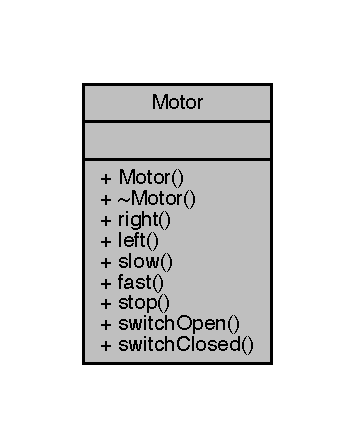
\includegraphics[width=170pt]{class_motor__coll__graph}
\end{center}
\end{figure}
\subsection*{Öffentliche Methoden}
\begin{DoxyCompactItemize}
\item 
\hyperlink{class_motor_a9150fc4647f7588364cb75dca1df4c96}{Motor} (\hyperlink{class_adapter}{Adapter} $\ast$adapt)
\item 
virtual \hyperlink{class_motor_a2e57c7b2681efea1d3b7f253ee88ecd4}{$\sim$\+Motor} ()
\item 
uint8\+\_\+t \hyperlink{class_motor_a517e585f6a9a335347f9a1230d2fc0e1}{right} ()
\item 
uint8\+\_\+t \hyperlink{class_motor_ae8af72c3a398bb959090d0be1083f5d7}{left} ()
\item 
uint8\+\_\+t \hyperlink{class_motor_a960a19729dc479265b1e5fea243de4c0}{slow} ()
\item 
uint8\+\_\+t \hyperlink{class_motor_a09b1a5376d1ea0eb39dff2ebcc325bde}{fast} ()
\item 
uint8\+\_\+t \hyperlink{class_motor_aab732159d4adf537bbcd3bcf9371d03b}{stop} ()
\item 
uint8\+\_\+t \hyperlink{class_motor_a35c0d7c6350b9f670dc243d31ea40263}{switch\+Open} ()
\item 
uint8\+\_\+t \hyperlink{class_motor_a38af68cbad8be09b85afc86f156f0f89}{switch\+Closed} ()
\end{DoxyCompactItemize}


\subsection{Beschreibung der Konstruktoren und Destruktoren}
\hypertarget{class_motor_a9150fc4647f7588364cb75dca1df4c96}{}\label{class_motor_a9150fc4647f7588364cb75dca1df4c96} 
\index{Motor@{Motor}!Motor@{Motor}}
\index{Motor@{Motor}!Motor@{Motor}}
\subsubsection{\texorpdfstring{Motor()}{Motor()}}
{\footnotesize\ttfamily Motor\+::\+Motor (\begin{DoxyParamCaption}\item[{\hyperlink{class_adapter}{Adapter} $\ast$}]{adapt }\end{DoxyParamCaption})}

\hypertarget{class_motor_a2e57c7b2681efea1d3b7f253ee88ecd4}{}\label{class_motor_a2e57c7b2681efea1d3b7f253ee88ecd4} 
\index{Motor@{Motor}!````~Motor@{$\sim$\+Motor}}
\index{````~Motor@{$\sim$\+Motor}!Motor@{Motor}}
\subsubsection{\texorpdfstring{$\sim$\+Motor()}{~Motor()}}
{\footnotesize\ttfamily Motor\+::$\sim$\+Motor (\begin{DoxyParamCaption}{ }\end{DoxyParamCaption})\hspace{0.3cm}{\ttfamily [virtual]}}



\subsection{Dokumentation der Elementfunktionen}
\hypertarget{class_motor_a09b1a5376d1ea0eb39dff2ebcc325bde}{}\label{class_motor_a09b1a5376d1ea0eb39dff2ebcc325bde} 
\index{Motor@{Motor}!fast@{fast}}
\index{fast@{fast}!Motor@{Motor}}
\subsubsection{\texorpdfstring{fast()}{fast()}}
{\footnotesize\ttfamily uint8\+\_\+t Motor\+::fast (\begin{DoxyParamCaption}{ }\end{DoxyParamCaption})}

\hypertarget{class_motor_ae8af72c3a398bb959090d0be1083f5d7}{}\label{class_motor_ae8af72c3a398bb959090d0be1083f5d7} 
\index{Motor@{Motor}!left@{left}}
\index{left@{left}!Motor@{Motor}}
\subsubsection{\texorpdfstring{left()}{left()}}
{\footnotesize\ttfamily uint8\+\_\+t Motor\+::left (\begin{DoxyParamCaption}{ }\end{DoxyParamCaption})}

\hypertarget{class_motor_a517e585f6a9a335347f9a1230d2fc0e1}{}\label{class_motor_a517e585f6a9a335347f9a1230d2fc0e1} 
\index{Motor@{Motor}!right@{right}}
\index{right@{right}!Motor@{Motor}}
\subsubsection{\texorpdfstring{right()}{right()}}
{\footnotesize\ttfamily uint8\+\_\+t Motor\+::right (\begin{DoxyParamCaption}{ }\end{DoxyParamCaption})}

\hypertarget{class_motor_a960a19729dc479265b1e5fea243de4c0}{}\label{class_motor_a960a19729dc479265b1e5fea243de4c0} 
\index{Motor@{Motor}!slow@{slow}}
\index{slow@{slow}!Motor@{Motor}}
\subsubsection{\texorpdfstring{slow()}{slow()}}
{\footnotesize\ttfamily uint8\+\_\+t Motor\+::slow (\begin{DoxyParamCaption}{ }\end{DoxyParamCaption})}

\hypertarget{class_motor_aab732159d4adf537bbcd3bcf9371d03b}{}\label{class_motor_aab732159d4adf537bbcd3bcf9371d03b} 
\index{Motor@{Motor}!stop@{stop}}
\index{stop@{stop}!Motor@{Motor}}
\subsubsection{\texorpdfstring{stop()}{stop()}}
{\footnotesize\ttfamily uint8\+\_\+t Motor\+::stop (\begin{DoxyParamCaption}{ }\end{DoxyParamCaption})}

\hypertarget{class_motor_a38af68cbad8be09b85afc86f156f0f89}{}\label{class_motor_a38af68cbad8be09b85afc86f156f0f89} 
\index{Motor@{Motor}!switch\+Closed@{switch\+Closed}}
\index{switch\+Closed@{switch\+Closed}!Motor@{Motor}}
\subsubsection{\texorpdfstring{switch\+Closed()}{switchClosed()}}
{\footnotesize\ttfamily uint8\+\_\+t Motor\+::switch\+Closed (\begin{DoxyParamCaption}{ }\end{DoxyParamCaption})}

\hypertarget{class_motor_a35c0d7c6350b9f670dc243d31ea40263}{}\label{class_motor_a35c0d7c6350b9f670dc243d31ea40263} 
\index{Motor@{Motor}!switch\+Open@{switch\+Open}}
\index{switch\+Open@{switch\+Open}!Motor@{Motor}}
\subsubsection{\texorpdfstring{switch\+Open()}{switchOpen()}}
{\footnotesize\ttfamily uint8\+\_\+t Motor\+::switch\+Open (\begin{DoxyParamCaption}{ }\end{DoxyParamCaption})}



Die Dokumentation für diese Klasse wurde erzeugt aufgrund der Dateien\+:\begin{DoxyCompactItemize}
\item 
Hal/\hyperlink{_motor_8h}{Motor.\+h}\item 
Hal/\hyperlink{_motor_8cpp}{Motor.\+cpp}\end{DoxyCompactItemize}

\hypertarget{class_mutexo}{}\section{Mutexo Klassenreferenz}
\label{class_mutexo}\index{Mutexo@{Mutexo}}


{\ttfamily \#include $<$Mutexo.\+h$>$}



Zusammengehörigkeiten von Mutexo\+:
\nopagebreak
\begin{figure}[H]
\begin{center}
\leavevmode
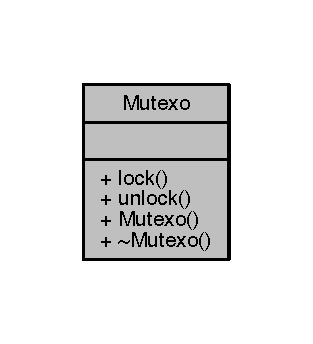
\includegraphics[width=150pt]{class_mutexo__coll__graph}
\end{center}
\end{figure}
\subsection*{Öffentliche Methoden}
\begin{DoxyCompactItemize}
\item 
int \hyperlink{class_mutexo_a22aac64070af68adc9acc1fef3d3f4aa}{lock} ()
\item 
int \hyperlink{class_mutexo_a9f51083616ed99edc2add313f840016c}{unlock} ()
\item 
\hyperlink{class_mutexo_a56f219370b120853d4176fb67a4fd847}{Mutexo} ()
\item 
virtual \hyperlink{class_mutexo_af8942ad328e7c91931f63e6a243081d1}{$\sim$\+Mutexo} ()
\end{DoxyCompactItemize}


\subsection{Beschreibung der Konstruktoren und Destruktoren}
\hypertarget{class_mutexo_a56f219370b120853d4176fb67a4fd847}{}\label{class_mutexo_a56f219370b120853d4176fb67a4fd847} 
\index{Mutexo@{Mutexo}!Mutexo@{Mutexo}}
\index{Mutexo@{Mutexo}!Mutexo@{Mutexo}}
\subsubsection{\texorpdfstring{Mutexo()}{Mutexo()}}
{\footnotesize\ttfamily Mutexo\+::\+Mutexo (\begin{DoxyParamCaption}{ }\end{DoxyParamCaption})}

\hypertarget{class_mutexo_af8942ad328e7c91931f63e6a243081d1}{}\label{class_mutexo_af8942ad328e7c91931f63e6a243081d1} 
\index{Mutexo@{Mutexo}!````~Mutexo@{$\sim$\+Mutexo}}
\index{````~Mutexo@{$\sim$\+Mutexo}!Mutexo@{Mutexo}}
\subsubsection{\texorpdfstring{$\sim$\+Mutexo()}{~Mutexo()}}
{\footnotesize\ttfamily Mutexo\+::$\sim$\+Mutexo (\begin{DoxyParamCaption}{ }\end{DoxyParamCaption})\hspace{0.3cm}{\ttfamily [virtual]}}



\subsection{Dokumentation der Elementfunktionen}
\hypertarget{class_mutexo_a22aac64070af68adc9acc1fef3d3f4aa}{}\label{class_mutexo_a22aac64070af68adc9acc1fef3d3f4aa} 
\index{Mutexo@{Mutexo}!lock@{lock}}
\index{lock@{lock}!Mutexo@{Mutexo}}
\subsubsection{\texorpdfstring{lock()}{lock()}}
{\footnotesize\ttfamily int Mutexo\+::lock (\begin{DoxyParamCaption}{ }\end{DoxyParamCaption})}

\hypertarget{class_mutexo_a9f51083616ed99edc2add313f840016c}{}\label{class_mutexo_a9f51083616ed99edc2add313f840016c} 
\index{Mutexo@{Mutexo}!unlock@{unlock}}
\index{unlock@{unlock}!Mutexo@{Mutexo}}
\subsubsection{\texorpdfstring{unlock()}{unlock()}}
{\footnotesize\ttfamily int Mutexo\+::unlock (\begin{DoxyParamCaption}{ }\end{DoxyParamCaption})}



Die Dokumentation für diese Klasse wurde erzeugt aufgrund der Dateien\+:\begin{DoxyCompactItemize}
\item 
/\+Users/marvin/conveyor/\+Projekt/\+Hal/\hyperlink{_mutexo_8h}{Mutexo.\+h}\item 
/\+Users/marvin/conveyor/\+Projekt/\+Hal/\hyperlink{_mutexo_8cpp}{Mutexo.\+cpp}\end{DoxyCompactItemize}

\hypertarget{struct_packet}{}\section{Packet Strukturreferenz}
\label{struct_packet}\index{Packet@{Packet}}


{\ttfamily \#include $<$Serial.\+h$>$}



Zusammengehörigkeiten von Packet\+:\nopagebreak
\begin{figure}[H]
\begin{center}
\leavevmode
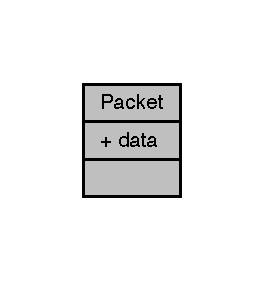
\includegraphics[width=127pt]{struct_packet__coll__graph}
\end{center}
\end{figure}
\subsection*{Öffentliche Attribute}
\begin{DoxyCompactItemize}
\item 
uint8\+\_\+t \hyperlink{struct_packet_a9c0a7fd8ec507914a389ed190ca3c51f}{data}
\end{DoxyCompactItemize}


\subsection{Dokumentation der Datenelemente}
\hypertarget{struct_packet_a9c0a7fd8ec507914a389ed190ca3c51f}{}\label{struct_packet_a9c0a7fd8ec507914a389ed190ca3c51f} 
\index{Packet@{Packet}!data@{data}}
\index{data@{data}!Packet@{Packet}}
\subsubsection{\texorpdfstring{data}{data}}
{\footnotesize\ttfamily uint8\+\_\+t Packet\+::data}



Die Dokumentation für diese Struktur wurde erzeugt aufgrund der Datei\+:\begin{DoxyCompactItemize}
\item 
Hal/\+Serial\+Interface/\hyperlink{_serial_8h}{Serial.\+h}\end{DoxyCompactItemize}

\hypertarget{class_parameter}{}\section{Parameter$<$ T $>$ Template-\/\+Klassenreferenz}
\label{class_parameter}\index{Parameter$<$ T $>$@{Parameter$<$ T $>$}}


{\ttfamily \#include $<$Parameter.\+h$>$}



Klassendiagramm für Parameter$<$ T $>$\+:\nopagebreak
\begin{figure}[H]
\begin{center}
\leavevmode
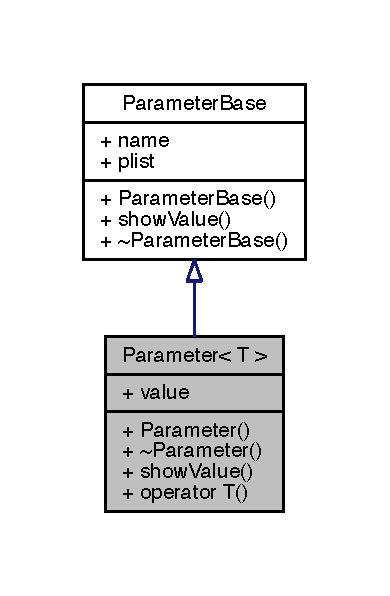
\includegraphics[width=187pt]{class_parameter__inherit__graph}
\end{center}
\end{figure}


Zusammengehörigkeiten von Parameter$<$ T $>$\+:\nopagebreak
\begin{figure}[H]
\begin{center}
\leavevmode
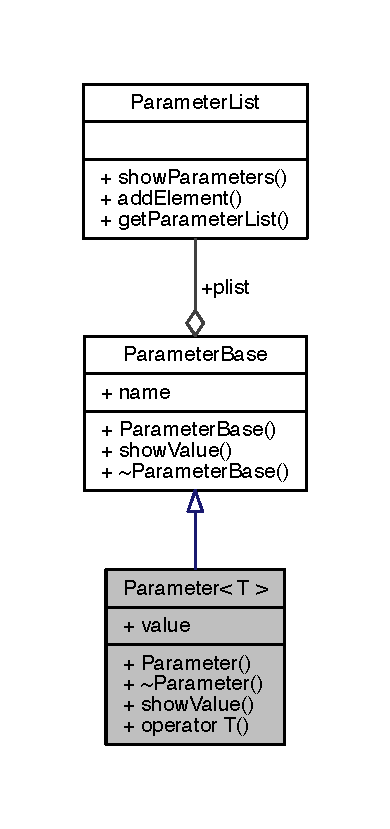
\includegraphics[width=187pt]{class_parameter__coll__graph}
\end{center}
\end{figure}
\subsection*{Öffentliche Methoden}
\begin{DoxyCompactItemize}
\item 
\hyperlink{class_parameter_a0043f636d495e3cd40686c35b0108059}{Parameter} (T v, std\+::string \hyperlink{class_parameter_base_a3e2e2ad34b89eabb0484b3a338133614}{name})
\item 
\hyperlink{class_parameter_a66e9872be5c4d3b49007c5be61ec5620}{$\sim$\+Parameter} ()
\item 
void \hyperlink{class_parameter_ab0091864db90216ee76ee9084422b380}{show\+Value} ()
\item 
\hyperlink{class_parameter_acd26e6a88234a14e642bfbcc8e3f5968}{operator T} () const
\end{DoxyCompactItemize}
\subsection*{Öffentliche Attribute}
\begin{DoxyCompactItemize}
\item 
T \hyperlink{class_parameter_a5dcbb3f478f204d7931eec2b3ed66117}{value}
\end{DoxyCompactItemize}


\subsection{Beschreibung der Konstruktoren und Destruktoren}
\hypertarget{class_parameter_a0043f636d495e3cd40686c35b0108059}{}\label{class_parameter_a0043f636d495e3cd40686c35b0108059} 
\index{Parameter@{Parameter}!Parameter@{Parameter}}
\index{Parameter@{Parameter}!Parameter@{Parameter}}
\subsubsection{\texorpdfstring{Parameter()}{Parameter()}}
{\footnotesize\ttfamily template$<$class T $>$ \\
\hyperlink{class_parameter}{Parameter}$<$ T $>$\+::\hyperlink{class_parameter}{Parameter} (\begin{DoxyParamCaption}\item[{T}]{v,  }\item[{std\+::string}]{name }\end{DoxyParamCaption})}

\hypertarget{class_parameter_a66e9872be5c4d3b49007c5be61ec5620}{}\label{class_parameter_a66e9872be5c4d3b49007c5be61ec5620} 
\index{Parameter@{Parameter}!````~Parameter@{$\sim$\+Parameter}}
\index{````~Parameter@{$\sim$\+Parameter}!Parameter@{Parameter}}
\subsubsection{\texorpdfstring{$\sim$\+Parameter()}{~Parameter()}}
{\footnotesize\ttfamily template$<$class T $>$ \\
\hyperlink{class_parameter}{Parameter}$<$ T $>$\+::$\sim$\hyperlink{class_parameter}{Parameter} (\begin{DoxyParamCaption}{ }\end{DoxyParamCaption})}



\subsection{Dokumentation der Elementfunktionen}
\hypertarget{class_parameter_acd26e6a88234a14e642bfbcc8e3f5968}{}\label{class_parameter_acd26e6a88234a14e642bfbcc8e3f5968} 
\index{Parameter@{Parameter}!operator T@{operator T}}
\index{operator T@{operator T}!Parameter@{Parameter}}
\subsubsection{\texorpdfstring{operator T()}{operator T()}}
{\footnotesize\ttfamily template$<$class T $>$ \\
\hyperlink{class_parameter}{Parameter}$<$ T $>$\+::operator T (\begin{DoxyParamCaption}{ }\end{DoxyParamCaption}) const\hspace{0.3cm}{\ttfamily [inline]}}

\hypertarget{class_parameter_ab0091864db90216ee76ee9084422b380}{}\label{class_parameter_ab0091864db90216ee76ee9084422b380} 
\index{Parameter@{Parameter}!show\+Value@{show\+Value}}
\index{show\+Value@{show\+Value}!Parameter@{Parameter}}
\subsubsection{\texorpdfstring{show\+Value()}{showValue()}}
{\footnotesize\ttfamily template$<$class T $>$ \\
void \hyperlink{class_parameter}{Parameter}$<$ T $>$\+::show\+Value (\begin{DoxyParamCaption}{ }\end{DoxyParamCaption})\hspace{0.3cm}{\ttfamily [virtual]}}



Implementiert \hyperlink{class_parameter_base_ad09b4d79a05987d903a7d97e16649df7}{Parameter\+Base}.



\subsection{Dokumentation der Datenelemente}
\hypertarget{class_parameter_a5dcbb3f478f204d7931eec2b3ed66117}{}\label{class_parameter_a5dcbb3f478f204d7931eec2b3ed66117} 
\index{Parameter@{Parameter}!value@{value}}
\index{value@{value}!Parameter@{Parameter}}
\subsubsection{\texorpdfstring{value}{value}}
{\footnotesize\ttfamily template$<$class T $>$ \\
T \hyperlink{class_parameter}{Parameter}$<$ T $>$\+::value}



Die Dokumentation für diese Klasse wurde erzeugt aufgrund der Datei\+:\begin{DoxyCompactItemize}
\item 
Config\+Management/\hyperlink{_parameter_8h}{Parameter.\+h}\end{DoxyCompactItemize}

\hypertarget{class_parameter_base}{}\section{Parameter\+Base Klassenreferenz}
\label{class_parameter_base}\index{Parameter\+Base@{Parameter\+Base}}


{\ttfamily \#include $<$Parameter\+Base.\+h$>$}



Klassendiagramm für Parameter\+Base\+:
\nopagebreak
\begin{figure}[H]
\begin{center}
\leavevmode
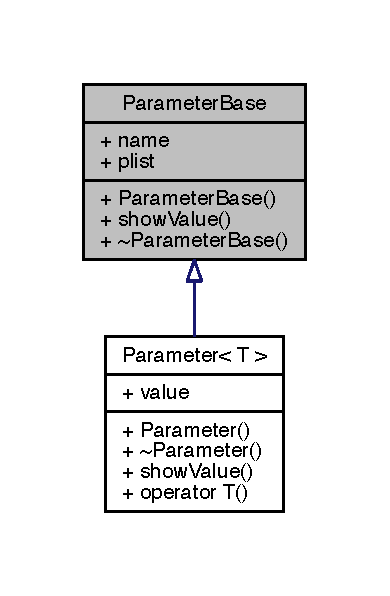
\includegraphics[width=187pt]{class_parameter_base__inherit__graph}
\end{center}
\end{figure}


Zusammengehörigkeiten von Parameter\+Base\+:
\nopagebreak
\begin{figure}[H]
\begin{center}
\leavevmode
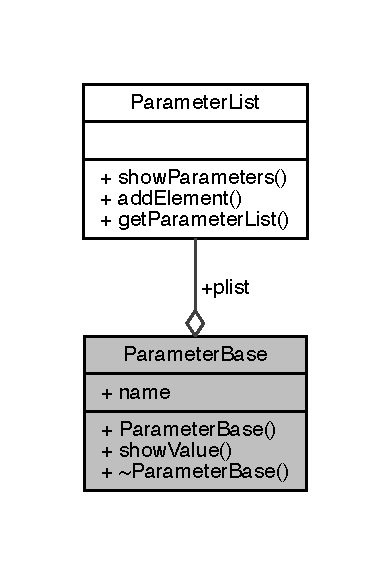
\includegraphics[width=187pt]{class_parameter_base__coll__graph}
\end{center}
\end{figure}
\subsection*{Öffentliche Methoden}
\begin{DoxyCompactItemize}
\item 
\hyperlink{class_parameter_base_aead2d4fe464a5ff7116704fe7581cf66}{Parameter\+Base} (std\+::string n)
\item 
virtual void \hyperlink{class_parameter_base_ad09b4d79a05987d903a7d97e16649df7}{show\+Value} ()=0
\item 
virtual \hyperlink{class_parameter_base_a93ff8a33fbfb1aa468e0f303c6449983}{$\sim$\+Parameter\+Base} ()
\end{DoxyCompactItemize}
\subsection*{Öffentliche Attribute}
\begin{DoxyCompactItemize}
\item 
std\+::string \hyperlink{class_parameter_base_a3e2e2ad34b89eabb0484b3a338133614}{name}
\item 
\hyperlink{class_parameter_list}{Parameter\+List} \& \hyperlink{class_parameter_base_a5fabd899cfe1b654e5ff3e93145dd461}{plist}
\end{DoxyCompactItemize}


\subsection{Beschreibung der Konstruktoren und Destruktoren}
\hypertarget{class_parameter_base_aead2d4fe464a5ff7116704fe7581cf66}{}\label{class_parameter_base_aead2d4fe464a5ff7116704fe7581cf66} 
\index{Parameter\+Base@{Parameter\+Base}!Parameter\+Base@{Parameter\+Base}}
\index{Parameter\+Base@{Parameter\+Base}!Parameter\+Base@{Parameter\+Base}}
\subsubsection{\texorpdfstring{Parameter\+Base()}{ParameterBase()}}
{\footnotesize\ttfamily Parameter\+Base\+::\+Parameter\+Base (\begin{DoxyParamCaption}\item[{std\+::string}]{n }\end{DoxyParamCaption})}

\hypertarget{class_parameter_base_a93ff8a33fbfb1aa468e0f303c6449983}{}\label{class_parameter_base_a93ff8a33fbfb1aa468e0f303c6449983} 
\index{Parameter\+Base@{Parameter\+Base}!````~Parameter\+Base@{$\sim$\+Parameter\+Base}}
\index{````~Parameter\+Base@{$\sim$\+Parameter\+Base}!Parameter\+Base@{Parameter\+Base}}
\subsubsection{\texorpdfstring{$\sim$\+Parameter\+Base()}{~ParameterBase()}}
{\footnotesize\ttfamily Parameter\+Base\+::$\sim$\+Parameter\+Base (\begin{DoxyParamCaption}{ }\end{DoxyParamCaption})\hspace{0.3cm}{\ttfamily [virtual]}}



\subsection{Dokumentation der Elementfunktionen}
\hypertarget{class_parameter_base_ad09b4d79a05987d903a7d97e16649df7}{}\label{class_parameter_base_ad09b4d79a05987d903a7d97e16649df7} 
\index{Parameter\+Base@{Parameter\+Base}!show\+Value@{show\+Value}}
\index{show\+Value@{show\+Value}!Parameter\+Base@{Parameter\+Base}}
\subsubsection{\texorpdfstring{show\+Value()}{showValue()}}
{\footnotesize\ttfamily virtual void Parameter\+Base\+::show\+Value (\begin{DoxyParamCaption}{ }\end{DoxyParamCaption})\hspace{0.3cm}{\ttfamily [pure virtual]}}



Implementiert in \hyperlink{class_parameter_ab0091864db90216ee76ee9084422b380}{Parameter$<$ T $>$}.



\subsection{Dokumentation der Datenelemente}
\hypertarget{class_parameter_base_a3e2e2ad34b89eabb0484b3a338133614}{}\label{class_parameter_base_a3e2e2ad34b89eabb0484b3a338133614} 
\index{Parameter\+Base@{Parameter\+Base}!name@{name}}
\index{name@{name}!Parameter\+Base@{Parameter\+Base}}
\subsubsection{\texorpdfstring{name}{name}}
{\footnotesize\ttfamily std\+::string Parameter\+Base\+::name}

\hypertarget{class_parameter_base_a5fabd899cfe1b654e5ff3e93145dd461}{}\label{class_parameter_base_a5fabd899cfe1b654e5ff3e93145dd461} 
\index{Parameter\+Base@{Parameter\+Base}!plist@{plist}}
\index{plist@{plist}!Parameter\+Base@{Parameter\+Base}}
\subsubsection{\texorpdfstring{plist}{plist}}
{\footnotesize\ttfamily \hyperlink{class_parameter_list}{Parameter\+List}\& Parameter\+Base\+::plist}



Die Dokumentation für diese Klasse wurde erzeugt aufgrund der Dateien\+:\begin{DoxyCompactItemize}
\item 
/\+Users/marvin/conveyor/\+Projekt/\+Config\+Management/\hyperlink{_parameter_base_8h}{Parameter\+Base.\+h}\item 
/\+Users/marvin/conveyor/\+Projekt/\+Config\+Management/\hyperlink{_parameter_base_8cpp}{Parameter\+Base.\+cpp}\end{DoxyCompactItemize}

\hypertarget{class_parameter_list}{}\section{Parameter\+List Klassenreferenz}
\label{class_parameter_list}\index{Parameter\+List@{Parameter\+List}}


{\ttfamily \#include $<$Parameter\+List.\+h$>$}



Zusammengehörigkeiten von Parameter\+List\+:
\nopagebreak
\begin{figure}[H]
\begin{center}
\leavevmode
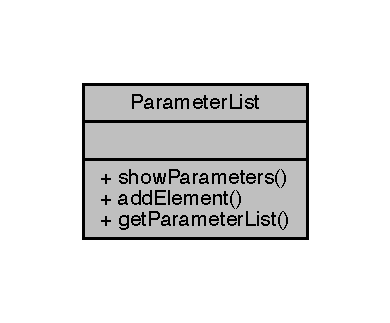
\includegraphics[width=187pt]{class_parameter_list__coll__graph}
\end{center}
\end{figure}
\subsection*{Öffentliche Methoden}
\begin{DoxyCompactItemize}
\item 
void \hyperlink{class_parameter_list_a8402f42970e27ac8618733f507178788}{show\+Parameters} ()
\item 
void \hyperlink{class_parameter_list_a4f4ede7252ae20641befa93cd6c316b3}{add\+Element} (\hyperlink{class_parameter_base}{Parameter\+Base} $\ast$parameter\+Base)
\end{DoxyCompactItemize}
\subsection*{Öffentliche, statische Methoden}
\begin{DoxyCompactItemize}
\item 
static \hyperlink{class_parameter_list}{Parameter\+List} \& \hyperlink{class_parameter_list_ae34f5f9c5a2c8cf9ea216cc733a0a68b}{get\+Parameter\+List} ()
\end{DoxyCompactItemize}


\subsection{Dokumentation der Elementfunktionen}
\hypertarget{class_parameter_list_a4f4ede7252ae20641befa93cd6c316b3}{}\label{class_parameter_list_a4f4ede7252ae20641befa93cd6c316b3} 
\index{Parameter\+List@{Parameter\+List}!add\+Element@{add\+Element}}
\index{add\+Element@{add\+Element}!Parameter\+List@{Parameter\+List}}
\subsubsection{\texorpdfstring{add\+Element()}{addElement()}}
{\footnotesize\ttfamily void Parameter\+List\+::add\+Element (\begin{DoxyParamCaption}\item[{\hyperlink{class_parameter_base}{Parameter\+Base} $\ast$}]{parameter\+Base }\end{DoxyParamCaption})}

\hypertarget{class_parameter_list_ae34f5f9c5a2c8cf9ea216cc733a0a68b}{}\label{class_parameter_list_ae34f5f9c5a2c8cf9ea216cc733a0a68b} 
\index{Parameter\+List@{Parameter\+List}!get\+Parameter\+List@{get\+Parameter\+List}}
\index{get\+Parameter\+List@{get\+Parameter\+List}!Parameter\+List@{Parameter\+List}}
\subsubsection{\texorpdfstring{get\+Parameter\+List()}{getParameterList()}}
{\footnotesize\ttfamily static \hyperlink{class_parameter_list}{Parameter\+List}\& Parameter\+List\+::get\+Parameter\+List (\begin{DoxyParamCaption}{ }\end{DoxyParamCaption})\hspace{0.3cm}{\ttfamily [inline]}, {\ttfamily [static]}}

\hypertarget{class_parameter_list_a8402f42970e27ac8618733f507178788}{}\label{class_parameter_list_a8402f42970e27ac8618733f507178788} 
\index{Parameter\+List@{Parameter\+List}!show\+Parameters@{show\+Parameters}}
\index{show\+Parameters@{show\+Parameters}!Parameter\+List@{Parameter\+List}}
\subsubsection{\texorpdfstring{show\+Parameters()}{showParameters()}}
{\footnotesize\ttfamily void Parameter\+List\+::show\+Parameters (\begin{DoxyParamCaption}{ }\end{DoxyParamCaption})}



Die Dokumentation für diese Klasse wurde erzeugt aufgrund der Dateien\+:\begin{DoxyCompactItemize}
\item 
/\+Users/marvin/conveyor/\+Projekt/\+Config\+Management/\hyperlink{_parameter_list_8h}{Parameter\+List.\+h}\item 
/\+Users/marvin/conveyor/\+Projekt/\+Config\+Management/\hyperlink{_parameter_list_8cpp}{Parameter\+List.\+cpp}\end{DoxyCompactItemize}

\hypertarget{class_serial}{}\section{Serial Klassenreferenz}
\label{class_serial}\index{Serial@{Serial}}


{\ttfamily \#include $<$Serial.\+h$>$}



Zusammengehörigkeiten von Serial\+:
\nopagebreak
\begin{figure}[H]
\begin{center}
\leavevmode
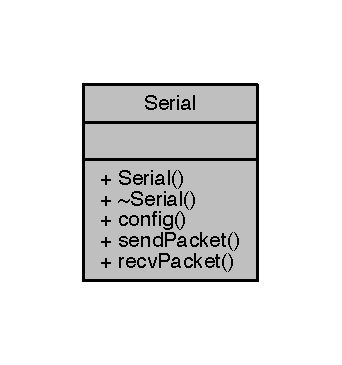
\includegraphics[width=164pt]{class_serial__coll__graph}
\end{center}
\end{figure}
\subsection*{Öffentliche Methoden}
\begin{DoxyCompactItemize}
\item 
\hyperlink{class_serial_a3667c3137f2df94716b5193f9fb736ab}{Serial} ()
\item 
\hyperlink{class_serial_a5b32c394c0ff923a4ef1c13cfb20a6ba}{$\sim$\+Serial} ()
\item 
void \hyperlink{class_serial_a50aa90466c7c87af0178cfd496da36be}{config} (void)
\item 
int \hyperlink{class_serial_a18fe9cf8fc366e6691b6ddf5e9b473a1}{send\+Packet} (\hyperlink{struct_packet}{Packet} $\ast$p)
\item 
int \hyperlink{class_serial_a357fce40e93f5a3700bfec09defd0bf9}{recv\+Packet} (\hyperlink{struct_packet}{Packet} $\ast$p)
\end{DoxyCompactItemize}


\subsection{Beschreibung der Konstruktoren und Destruktoren}
\hypertarget{class_serial_a3667c3137f2df94716b5193f9fb736ab}{}\label{class_serial_a3667c3137f2df94716b5193f9fb736ab} 
\index{Serial@{Serial}!Serial@{Serial}}
\index{Serial@{Serial}!Serial@{Serial}}
\subsubsection{\texorpdfstring{Serial()}{Serial()}}
{\footnotesize\ttfamily Serial\+::\+Serial (\begin{DoxyParamCaption}{ }\end{DoxyParamCaption})}

\hypertarget{class_serial_a5b32c394c0ff923a4ef1c13cfb20a6ba}{}\label{class_serial_a5b32c394c0ff923a4ef1c13cfb20a6ba} 
\index{Serial@{Serial}!````~Serial@{$\sim$\+Serial}}
\index{````~Serial@{$\sim$\+Serial}!Serial@{Serial}}
\subsubsection{\texorpdfstring{$\sim$\+Serial()}{~Serial()}}
{\footnotesize\ttfamily Serial\+::$\sim$\+Serial (\begin{DoxyParamCaption}{ }\end{DoxyParamCaption})}



\subsection{Dokumentation der Elementfunktionen}
\hypertarget{class_serial_a50aa90466c7c87af0178cfd496da36be}{}\label{class_serial_a50aa90466c7c87af0178cfd496da36be} 
\index{Serial@{Serial}!config@{config}}
\index{config@{config}!Serial@{Serial}}
\subsubsection{\texorpdfstring{config()}{config()}}
{\footnotesize\ttfamily void Serial\+::config (\begin{DoxyParamCaption}\item[{void}]{ }\end{DoxyParamCaption})}

\hypertarget{class_serial_a357fce40e93f5a3700bfec09defd0bf9}{}\label{class_serial_a357fce40e93f5a3700bfec09defd0bf9} 
\index{Serial@{Serial}!recv\+Packet@{recv\+Packet}}
\index{recv\+Packet@{recv\+Packet}!Serial@{Serial}}
\subsubsection{\texorpdfstring{recv\+Packet()}{recvPacket()}}
{\footnotesize\ttfamily int Serial\+::recv\+Packet (\begin{DoxyParamCaption}\item[{\hyperlink{struct_packet}{Packet} $\ast$}]{p }\end{DoxyParamCaption})}

\hypertarget{class_serial_a18fe9cf8fc366e6691b6ddf5e9b473a1}{}\label{class_serial_a18fe9cf8fc366e6691b6ddf5e9b473a1} 
\index{Serial@{Serial}!send\+Packet@{send\+Packet}}
\index{send\+Packet@{send\+Packet}!Serial@{Serial}}
\subsubsection{\texorpdfstring{send\+Packet()}{sendPacket()}}
{\footnotesize\ttfamily int Serial\+::send\+Packet (\begin{DoxyParamCaption}\item[{\hyperlink{struct_packet}{Packet} $\ast$}]{p }\end{DoxyParamCaption})}



Die Dokumentation für diese Klasse wurde erzeugt aufgrund der Dateien\+:\begin{DoxyCompactItemize}
\item 
/\+Users/marvin/conveyor/\+Projekt/\+Hal/\+Serial\+Interface/\hyperlink{_serial_8h}{Serial.\+h}\item 
/\+Users/marvin/conveyor/\+Projekt/\+Hal/\+Serial\+Interface/\hyperlink{_serial_8cpp}{Serial.\+cpp}\end{DoxyCompactItemize}

\hypertarget{class_serializer}{}\section{Serializer Klassenreferenz}
\label{class_serializer}\index{Serializer@{Serializer}}


{\ttfamily \#include $<$Serializer.\+h$>$}



Zusammengehörigkeiten von Serializer\+:\nopagebreak
\begin{figure}[H]
\begin{center}
\leavevmode
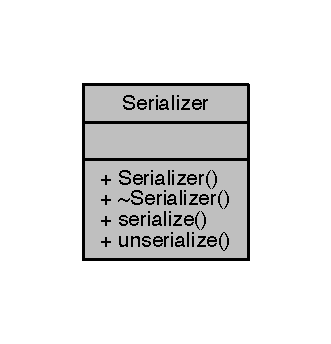
\includegraphics[width=159pt]{class_serializer__coll__graph}
\end{center}
\end{figure}
\subsection*{Öffentliche Methoden}
\begin{DoxyCompactItemize}
\item 
\hyperlink{class_serializer_a9fe7f31924098f75278d059f8443fd5b}{Serializer} ()
\item 
\hyperlink{class_serializer_a42a7d2d8e622ad1ef5f869813b498aa9}{$\sim$\+Serializer} ()
\item 
std\+::string \hyperlink{class_serializer_a76490c3d7c31f10cd2c991731fd54ac5}{serialize} ()
\item 
std\+::string \hyperlink{class_serializer_a55d2d0ca552d5a14b316bab0d8f1590a}{unserialize} ()
\end{DoxyCompactItemize}


\subsection{Beschreibung der Konstruktoren und Destruktoren}
\hypertarget{class_serializer_a9fe7f31924098f75278d059f8443fd5b}{}\label{class_serializer_a9fe7f31924098f75278d059f8443fd5b} 
\index{Serializer@{Serializer}!Serializer@{Serializer}}
\index{Serializer@{Serializer}!Serializer@{Serializer}}
\subsubsection{\texorpdfstring{Serializer()}{Serializer()}}
{\footnotesize\ttfamily Serializer\+::\+Serializer (\begin{DoxyParamCaption}{ }\end{DoxyParamCaption})}

\hypertarget{class_serializer_a42a7d2d8e622ad1ef5f869813b498aa9}{}\label{class_serializer_a42a7d2d8e622ad1ef5f869813b498aa9} 
\index{Serializer@{Serializer}!````~Serializer@{$\sim$\+Serializer}}
\index{````~Serializer@{$\sim$\+Serializer}!Serializer@{Serializer}}
\subsubsection{\texorpdfstring{$\sim$\+Serializer()}{~Serializer()}}
{\footnotesize\ttfamily Serializer\+::$\sim$\+Serializer (\begin{DoxyParamCaption}{ }\end{DoxyParamCaption})}



\subsection{Dokumentation der Elementfunktionen}
\hypertarget{class_serializer_a76490c3d7c31f10cd2c991731fd54ac5}{}\label{class_serializer_a76490c3d7c31f10cd2c991731fd54ac5} 
\index{Serializer@{Serializer}!serialize@{serialize}}
\index{serialize@{serialize}!Serializer@{Serializer}}
\subsubsection{\texorpdfstring{serialize()}{serialize()}}
{\footnotesize\ttfamily std\+::string Serializer\+::serialize (\begin{DoxyParamCaption}{ }\end{DoxyParamCaption})}

\hypertarget{class_serializer_a55d2d0ca552d5a14b316bab0d8f1590a}{}\label{class_serializer_a55d2d0ca552d5a14b316bab0d8f1590a} 
\index{Serializer@{Serializer}!unserialize@{unserialize}}
\index{unserialize@{unserialize}!Serializer@{Serializer}}
\subsubsection{\texorpdfstring{unserialize()}{unserialize()}}
{\footnotesize\ttfamily std\+::string Serializer\+::unserialize (\begin{DoxyParamCaption}{ }\end{DoxyParamCaption})}



Die Dokumentation für diese Klasse wurde erzeugt aufgrund der Dateien\+:\begin{DoxyCompactItemize}
\item 
Serializer/\hyperlink{_serializer_8h}{Serializer.\+h}\item 
Serializer/\hyperlink{_serializer_8cpp}{Serializer.\+cpp}\end{DoxyCompactItemize}

\hypertarget{class_serializer_adapter}{}\section{Serializer\+Adapter$<$ T $>$ Template-\/\+Klassenreferenz}
\label{class_serializer_adapter}\index{Serializer\+Adapter$<$ T $>$@{Serializer\+Adapter$<$ T $>$}}


{\ttfamily \#include $<$Serializer\+Adapter.\+h$>$}



Zusammengehörigkeiten von Serializer\+Adapter$<$ T $>$\+:
\nopagebreak
\begin{figure}[H]
\begin{center}
\leavevmode
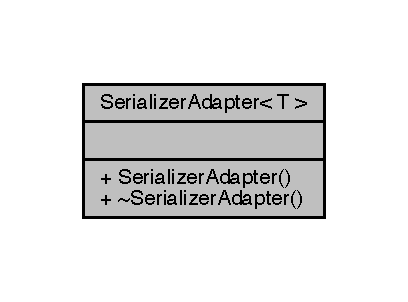
\includegraphics[width=196pt]{class_serializer_adapter__coll__graph}
\end{center}
\end{figure}
\subsection*{Öffentliche Methoden}
\begin{DoxyCompactItemize}
\item 
\hyperlink{class_serializer_adapter_ac815cf2eb9414d93eae850d1d31c7120}{Serializer\+Adapter} ()
\item 
virtual \hyperlink{class_serializer_adapter_ab768851e14fa435e50f4d39faacaea89}{$\sim$\+Serializer\+Adapter} ()
\end{DoxyCompactItemize}


\subsection{Beschreibung der Konstruktoren und Destruktoren}
\hypertarget{class_serializer_adapter_ac815cf2eb9414d93eae850d1d31c7120}{}\label{class_serializer_adapter_ac815cf2eb9414d93eae850d1d31c7120} 
\index{Serializer\+Adapter@{Serializer\+Adapter}!Serializer\+Adapter@{Serializer\+Adapter}}
\index{Serializer\+Adapter@{Serializer\+Adapter}!Serializer\+Adapter@{Serializer\+Adapter}}
\subsubsection{\texorpdfstring{Serializer\+Adapter()}{SerializerAdapter()}}
{\footnotesize\ttfamily template$<$class T $>$ \\
\hyperlink{class_serializer_adapter}{Serializer\+Adapter}$<$ T $>$\+::\hyperlink{class_serializer_adapter}{Serializer\+Adapter} (\begin{DoxyParamCaption}{ }\end{DoxyParamCaption})}

\hypertarget{class_serializer_adapter_ab768851e14fa435e50f4d39faacaea89}{}\label{class_serializer_adapter_ab768851e14fa435e50f4d39faacaea89} 
\index{Serializer\+Adapter@{Serializer\+Adapter}!````~Serializer\+Adapter@{$\sim$\+Serializer\+Adapter}}
\index{````~Serializer\+Adapter@{$\sim$\+Serializer\+Adapter}!Serializer\+Adapter@{Serializer\+Adapter}}
\subsubsection{\texorpdfstring{$\sim$\+Serializer\+Adapter()}{~SerializerAdapter()}}
{\footnotesize\ttfamily template$<$class T $>$ \\
\hyperlink{class_serializer_adapter}{Serializer\+Adapter}$<$ T $>$\+::$\sim$\hyperlink{class_serializer_adapter}{Serializer\+Adapter} (\begin{DoxyParamCaption}{ }\end{DoxyParamCaption})\hspace{0.3cm}{\ttfamily [virtual]}}



Die Dokumentation für diese Klasse wurde erzeugt aufgrund der Dateien\+:\begin{DoxyCompactItemize}
\item 
/\+Users/marvin/conveyor/\+Projekt/\+Serializer/\hyperlink{_serializer_adapter_8h}{Serializer\+Adapter.\+h}\item 
/\+Users/marvin/conveyor/\+Projekt/\+Serializer/\hyperlink{_serializer_adapter_8cpp}{Serializer\+Adapter.\+cpp}\end{DoxyCompactItemize}

\hypertarget{class_serializer_interface}{}\section{Serializer\+Interface Klassenreferenz}
\label{class_serializer_interface}\index{Serializer\+Interface@{Serializer\+Interface}}


{\ttfamily \#include $<$Serializer\+Interface.\+h$>$}



Zusammengehörigkeiten von Serializer\+Interface\+:\nopagebreak
\begin{figure}[H]
\begin{center}
\leavevmode
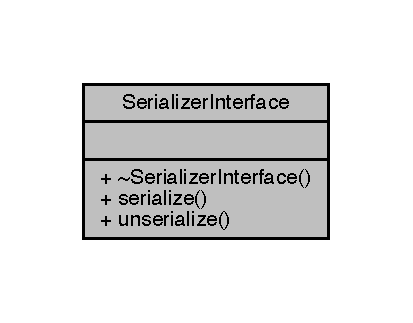
\includegraphics[width=198pt]{class_serializer_interface__coll__graph}
\end{center}
\end{figure}
\subsection*{Öffentliche Methoden}
\begin{DoxyCompactItemize}
\item 
virtual \hyperlink{class_serializer_interface_aea8141688fdd8721b178c181d25820e2}{$\sim$\+Serializer\+Interface} ()
\item 
virtual std\+::string \hyperlink{class_serializer_interface_a7ca657af272daca5396afd0c53f845a5}{serialize} ()=0
\item 
virtual std\+::string \hyperlink{class_serializer_interface_a0d3718721a1b03be94e5b3efb09c9f7b}{unserialize} ()=0
\end{DoxyCompactItemize}


\subsection{Beschreibung der Konstruktoren und Destruktoren}
\hypertarget{class_serializer_interface_aea8141688fdd8721b178c181d25820e2}{}\label{class_serializer_interface_aea8141688fdd8721b178c181d25820e2} 
\index{Serializer\+Interface@{Serializer\+Interface}!````~Serializer\+Interface@{$\sim$\+Serializer\+Interface}}
\index{````~Serializer\+Interface@{$\sim$\+Serializer\+Interface}!Serializer\+Interface@{Serializer\+Interface}}
\subsubsection{\texorpdfstring{$\sim$\+Serializer\+Interface()}{~SerializerInterface()}}
{\footnotesize\ttfamily virtual Serializer\+Interface\+::$\sim$\+Serializer\+Interface (\begin{DoxyParamCaption}{ }\end{DoxyParamCaption})\hspace{0.3cm}{\ttfamily [virtual]}}



\subsection{Dokumentation der Elementfunktionen}
\hypertarget{class_serializer_interface_a7ca657af272daca5396afd0c53f845a5}{}\label{class_serializer_interface_a7ca657af272daca5396afd0c53f845a5} 
\index{Serializer\+Interface@{Serializer\+Interface}!serialize@{serialize}}
\index{serialize@{serialize}!Serializer\+Interface@{Serializer\+Interface}}
\subsubsection{\texorpdfstring{serialize()}{serialize()}}
{\footnotesize\ttfamily virtual std\+::string Serializer\+Interface\+::serialize (\begin{DoxyParamCaption}{ }\end{DoxyParamCaption})\hspace{0.3cm}{\ttfamily [pure virtual]}}

\hypertarget{class_serializer_interface_a0d3718721a1b03be94e5b3efb09c9f7b}{}\label{class_serializer_interface_a0d3718721a1b03be94e5b3efb09c9f7b} 
\index{Serializer\+Interface@{Serializer\+Interface}!unserialize@{unserialize}}
\index{unserialize@{unserialize}!Serializer\+Interface@{Serializer\+Interface}}
\subsubsection{\texorpdfstring{unserialize()}{unserialize()}}
{\footnotesize\ttfamily virtual std\+::string Serializer\+Interface\+::unserialize (\begin{DoxyParamCaption}{ }\end{DoxyParamCaption})\hspace{0.3cm}{\ttfamily [pure virtual]}}



Die Dokumentation für diese Klasse wurde erzeugt aufgrund der Datei\+:\begin{DoxyCompactItemize}
\item 
Serializer/\hyperlink{_serializer_interface_8h}{Serializer\+Interface.\+h}\end{DoxyCompactItemize}

\hypertarget{class_serial_message}{}\section{Serial\+Message Klassenreferenz}
\label{class_serial_message}\index{Serial\+Message@{Serial\+Message}}


{\ttfamily \#include $<$Serial\+Message.\+h$>$}



Zusammengehörigkeiten von Serial\+Message\+:\nopagebreak
\begin{figure}[H]
\begin{center}
\leavevmode
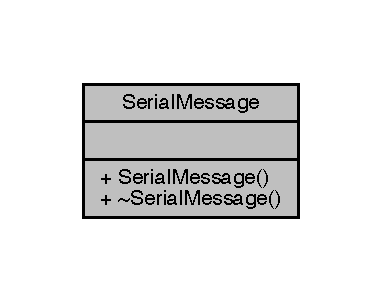
\includegraphics[width=183pt]{class_serial_message__coll__graph}
\end{center}
\end{figure}
\subsection*{Öffentliche Methoden}
\begin{DoxyCompactItemize}
\item 
\hyperlink{class_serial_message_aef84d2a1b8928bf39c0f4e59bdf7e36f}{Serial\+Message} ()
\item 
virtual \hyperlink{class_serial_message_a9bcc2b473a850ca82bf139a9fee6debb}{$\sim$\+Serial\+Message} ()
\end{DoxyCompactItemize}


\subsection{Beschreibung der Konstruktoren und Destruktoren}
\hypertarget{class_serial_message_aef84d2a1b8928bf39c0f4e59bdf7e36f}{}\label{class_serial_message_aef84d2a1b8928bf39c0f4e59bdf7e36f} 
\index{Serial\+Message@{Serial\+Message}!Serial\+Message@{Serial\+Message}}
\index{Serial\+Message@{Serial\+Message}!Serial\+Message@{Serial\+Message}}
\subsubsection{\texorpdfstring{Serial\+Message()}{SerialMessage()}}
{\footnotesize\ttfamily Serial\+Message\+::\+Serial\+Message (\begin{DoxyParamCaption}{ }\end{DoxyParamCaption})}

\hypertarget{class_serial_message_a9bcc2b473a850ca82bf139a9fee6debb}{}\label{class_serial_message_a9bcc2b473a850ca82bf139a9fee6debb} 
\index{Serial\+Message@{Serial\+Message}!````~Serial\+Message@{$\sim$\+Serial\+Message}}
\index{````~Serial\+Message@{$\sim$\+Serial\+Message}!Serial\+Message@{Serial\+Message}}
\subsubsection{\texorpdfstring{$\sim$\+Serial\+Message()}{~SerialMessage()}}
{\footnotesize\ttfamily Serial\+Message\+::$\sim$\+Serial\+Message (\begin{DoxyParamCaption}{ }\end{DoxyParamCaption})\hspace{0.3cm}{\ttfamily [virtual]}}



Die Dokumentation für diese Klasse wurde erzeugt aufgrund der Dateien\+:\begin{DoxyCompactItemize}
\item 
Entity/\hyperlink{_serial_message_8h}{Serial\+Message.\+h}\item 
Entity/\hyperlink{_serial_message_8cpp}{Serial\+Message.\+cpp}\end{DoxyCompactItemize}

\hypertarget{class_serial_thread}{}\section{Serial\+Thread Klassenreferenz}
\label{class_serial_thread}\index{Serial\+Thread@{Serial\+Thread}}


{\ttfamily \#include $<$Serial\+Thread.\+h$>$}



Zusammengehörigkeiten von Serial\+Thread\+:\nopagebreak
\begin{figure}[H]
\begin{center}
\leavevmode
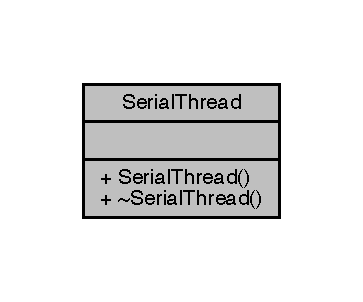
\includegraphics[width=174pt]{class_serial_thread__coll__graph}
\end{center}
\end{figure}
\subsection*{Öffentliche Methoden}
\begin{DoxyCompactItemize}
\item 
\hyperlink{class_serial_thread_a4adb81a5e8a3246f41554d72ca7062d4}{Serial\+Thread} ()
\item 
virtual \hyperlink{class_serial_thread_a14eabc004344a056196fa093189d9406}{$\sim$\+Serial\+Thread} ()
\end{DoxyCompactItemize}


\subsection{Beschreibung der Konstruktoren und Destruktoren}
\hypertarget{class_serial_thread_a4adb81a5e8a3246f41554d72ca7062d4}{}\label{class_serial_thread_a4adb81a5e8a3246f41554d72ca7062d4} 
\index{Serial\+Thread@{Serial\+Thread}!Serial\+Thread@{Serial\+Thread}}
\index{Serial\+Thread@{Serial\+Thread}!Serial\+Thread@{Serial\+Thread}}
\subsubsection{\texorpdfstring{Serial\+Thread()}{SerialThread()}}
{\footnotesize\ttfamily Serial\+Thread\+::\+Serial\+Thread (\begin{DoxyParamCaption}{ }\end{DoxyParamCaption})}

\hypertarget{class_serial_thread_a14eabc004344a056196fa093189d9406}{}\label{class_serial_thread_a14eabc004344a056196fa093189d9406} 
\index{Serial\+Thread@{Serial\+Thread}!````~Serial\+Thread@{$\sim$\+Serial\+Thread}}
\index{````~Serial\+Thread@{$\sim$\+Serial\+Thread}!Serial\+Thread@{Serial\+Thread}}
\subsubsection{\texorpdfstring{$\sim$\+Serial\+Thread()}{~SerialThread()}}
{\footnotesize\ttfamily Serial\+Thread\+::$\sim$\+Serial\+Thread (\begin{DoxyParamCaption}{ }\end{DoxyParamCaption})\hspace{0.3cm}{\ttfamily [virtual]}}



Die Dokumentation für diese Klasse wurde erzeugt aufgrund der Dateien\+:\begin{DoxyCompactItemize}
\item 
test/\hyperlink{_serial_thread_8h}{Serial\+Thread.\+h}\item 
test/\hyperlink{_serial_thread_8cpp}{Serial\+Thread.\+cpp}\end{DoxyCompactItemize}

\hypertarget{class_signal_handler_thread}{}\section{Signal\+Handler\+Thread Klassenreferenz}
\label{class_signal_handler_thread}\index{Signal\+Handler\+Thread@{Signal\+Handler\+Thread}}


{\ttfamily \#include $<$Signal\+Handler\+Thread.\+h$>$}



Klassendiagramm für Signal\+Handler\+Thread\+:\nopagebreak
\begin{figure}[H]
\begin{center}
\leavevmode
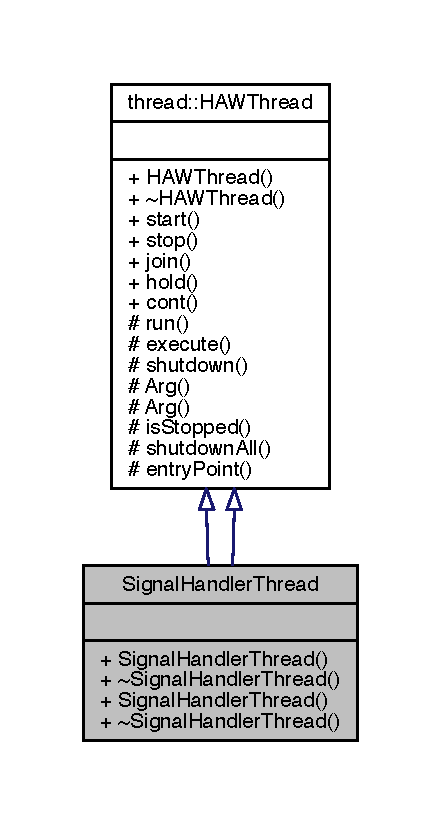
\includegraphics[width=212pt]{class_signal_handler_thread__inherit__graph}
\end{center}
\end{figure}


Zusammengehörigkeiten von Signal\+Handler\+Thread\+:\nopagebreak
\begin{figure}[H]
\begin{center}
\leavevmode
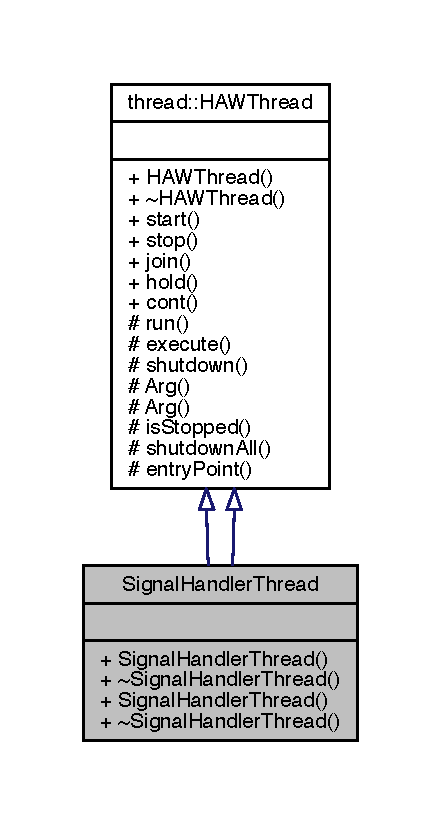
\includegraphics[width=212pt]{class_signal_handler_thread__coll__graph}
\end{center}
\end{figure}
\subsection*{Öffentliche Methoden}
\begin{DoxyCompactItemize}
\item 
\hyperlink{class_signal_handler_thread_ab78029caf852fcaa1d4c1d22ae1432fd}{Signal\+Handler\+Thread} ()
\item 
virtual \hyperlink{class_signal_handler_thread_a414c6ca3b03db6f0fa9bf24957421bf4}{$\sim$\+Signal\+Handler\+Thread} ()
\item 
\hyperlink{class_signal_handler_thread_ab78029caf852fcaa1d4c1d22ae1432fd}{Signal\+Handler\+Thread} ()
\item 
virtual \hyperlink{class_signal_handler_thread_ae5f82b0b55704aba1cbf0e06002b2737}{$\sim$\+Signal\+Handler\+Thread} ()
\end{DoxyCompactItemize}
\subsection*{Weitere Geerbte Elemente}


\subsection{Beschreibung der Konstruktoren und Destruktoren}
\hypertarget{class_signal_handler_thread_ab78029caf852fcaa1d4c1d22ae1432fd}{}\label{class_signal_handler_thread_ab78029caf852fcaa1d4c1d22ae1432fd} 
\index{Signal\+Handler\+Thread@{Signal\+Handler\+Thread}!Signal\+Handler\+Thread@{Signal\+Handler\+Thread}}
\index{Signal\+Handler\+Thread@{Signal\+Handler\+Thread}!Signal\+Handler\+Thread@{Signal\+Handler\+Thread}}
\subsubsection{\texorpdfstring{Signal\+Handler\+Thread()}{SignalHandlerThread()}\hspace{0.1cm}{\footnotesize\ttfamily [1/2]}}
{\footnotesize\ttfamily Signal\+Handler\+Thread\+::\+Signal\+Handler\+Thread (\begin{DoxyParamCaption}{ }\end{DoxyParamCaption})}

\hypertarget{class_signal_handler_thread_a414c6ca3b03db6f0fa9bf24957421bf4}{}\label{class_signal_handler_thread_a414c6ca3b03db6f0fa9bf24957421bf4} 
\index{Signal\+Handler\+Thread@{Signal\+Handler\+Thread}!````~Signal\+Handler\+Thread@{$\sim$\+Signal\+Handler\+Thread}}
\index{````~Signal\+Handler\+Thread@{$\sim$\+Signal\+Handler\+Thread}!Signal\+Handler\+Thread@{Signal\+Handler\+Thread}}
\subsubsection{\texorpdfstring{$\sim$\+Signal\+Handler\+Thread()}{~SignalHandlerThread()}\hspace{0.1cm}{\footnotesize\ttfamily [1/2]}}
{\footnotesize\ttfamily Signal\+Handler\+Thread\+::$\sim$\+Signal\+Handler\+Thread (\begin{DoxyParamCaption}{ }\end{DoxyParamCaption})\hspace{0.3cm}{\ttfamily [virtual]}}

\hypertarget{class_signal_handler_thread_ab78029caf852fcaa1d4c1d22ae1432fd}{}\label{class_signal_handler_thread_ab78029caf852fcaa1d4c1d22ae1432fd} 
\index{Signal\+Handler\+Thread@{Signal\+Handler\+Thread}!Signal\+Handler\+Thread@{Signal\+Handler\+Thread}}
\index{Signal\+Handler\+Thread@{Signal\+Handler\+Thread}!Signal\+Handler\+Thread@{Signal\+Handler\+Thread}}
\subsubsection{\texorpdfstring{Signal\+Handler\+Thread()}{SignalHandlerThread()}\hspace{0.1cm}{\footnotesize\ttfamily [2/2]}}
{\footnotesize\ttfamily Signal\+Handler\+Thread\+::\+Signal\+Handler\+Thread (\begin{DoxyParamCaption}{ }\end{DoxyParamCaption})}

\hypertarget{class_signal_handler_thread_ae5f82b0b55704aba1cbf0e06002b2737}{}\label{class_signal_handler_thread_ae5f82b0b55704aba1cbf0e06002b2737} 
\index{Signal\+Handler\+Thread@{Signal\+Handler\+Thread}!````~Signal\+Handler\+Thread@{$\sim$\+Signal\+Handler\+Thread}}
\index{````~Signal\+Handler\+Thread@{$\sim$\+Signal\+Handler\+Thread}!Signal\+Handler\+Thread@{Signal\+Handler\+Thread}}
\subsubsection{\texorpdfstring{$\sim$\+Signal\+Handler\+Thread()}{~SignalHandlerThread()}\hspace{0.1cm}{\footnotesize\ttfamily [2/2]}}
{\footnotesize\ttfamily virtual Signal\+Handler\+Thread\+::$\sim$\+Signal\+Handler\+Thread (\begin{DoxyParamCaption}{ }\end{DoxyParamCaption})\hspace{0.3cm}{\ttfamily [virtual]}}



Die Dokumentation für diese Klasse wurde erzeugt aufgrund der Dateien\+:\begin{DoxyCompactItemize}
\item 
test/\+H\+A\+L/\+Sensorik/\hyperlink{test_2_h_a_l_2_sensorik_2_signal_handler_thread_8h}{Signal\+Handler\+Thread.\+h}\item 
test/\+H\+A\+L/\+Sensorik/\hyperlink{test_2_h_a_l_2_sensorik_2_signal_handler_thread_8cpp}{Signal\+Handler\+Thread.\+cpp}\end{DoxyCompactItemize}

\hypertarget{class_traffic_light}{}\section{Traffic\+Light Klassenreferenz}
\label{class_traffic_light}\index{Traffic\+Light@{Traffic\+Light}}


{\ttfamily \#include $<$Traffic\+Light.\+h$>$}



Zusammengehörigkeiten von Traffic\+Light\+:\nopagebreak
\begin{figure}[H]
\begin{center}
\leavevmode
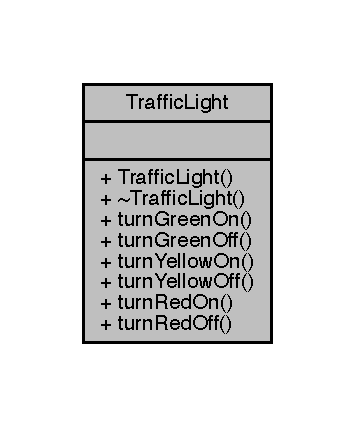
\includegraphics[width=170pt]{class_traffic_light__coll__graph}
\end{center}
\end{figure}
\subsection*{Öffentliche Methoden}
\begin{DoxyCompactItemize}
\item 
\hyperlink{class_traffic_light_ac34af2ea06577584a1c30a4f40e2d521}{Traffic\+Light} (\hyperlink{class_adapter}{Adapter} $\ast$adapt)
\item 
\hyperlink{class_traffic_light_a3dd2a89a028c1586ced0ab587dda8cc1}{$\sim$\+Traffic\+Light} ()
\item 
uint8\+\_\+t \hyperlink{class_traffic_light_a9477c1e61facd79e308b297877e3beee}{turn\+Green\+On} ()
\item 
uint8\+\_\+t \hyperlink{class_traffic_light_a958814eefaf288da1e103bf32c5c38b9}{turn\+Green\+Off} ()
\item 
uint8\+\_\+t \hyperlink{class_traffic_light_a74b400dafd029a2cfde6c27434111d21}{turn\+Yellow\+On} ()
\item 
uint8\+\_\+t \hyperlink{class_traffic_light_a17723c3478b4eb754aa8b163234aa8be}{turn\+Yellow\+Off} ()
\item 
uint8\+\_\+t \hyperlink{class_traffic_light_acd3d36d6884744b2230bd234bff27357}{turn\+Red\+On} ()
\item 
uint8\+\_\+t \hyperlink{class_traffic_light_a2ca2808ea156abc199a14939c2ab0c92}{turn\+Red\+Off} ()
\end{DoxyCompactItemize}


\subsection{Beschreibung der Konstruktoren und Destruktoren}
\hypertarget{class_traffic_light_ac34af2ea06577584a1c30a4f40e2d521}{}\label{class_traffic_light_ac34af2ea06577584a1c30a4f40e2d521} 
\index{Traffic\+Light@{Traffic\+Light}!Traffic\+Light@{Traffic\+Light}}
\index{Traffic\+Light@{Traffic\+Light}!Traffic\+Light@{Traffic\+Light}}
\subsubsection{\texorpdfstring{Traffic\+Light()}{TrafficLight()}}
{\footnotesize\ttfamily Traffic\+Light\+::\+Traffic\+Light (\begin{DoxyParamCaption}\item[{\hyperlink{class_adapter}{Adapter} $\ast$}]{adapt }\end{DoxyParamCaption})}

Constructor der Ampel


\begin{DoxyParams}{Parameter}
{\em adapt} & \hyperlink{class_adapter}{Adapter} für die Steuerung der Ampel. \\
\hline
\end{DoxyParams}
\hypertarget{class_traffic_light_a3dd2a89a028c1586ced0ab587dda8cc1}{}\label{class_traffic_light_a3dd2a89a028c1586ced0ab587dda8cc1} 
\index{Traffic\+Light@{Traffic\+Light}!````~Traffic\+Light@{$\sim$\+Traffic\+Light}}
\index{````~Traffic\+Light@{$\sim$\+Traffic\+Light}!Traffic\+Light@{Traffic\+Light}}
\subsubsection{\texorpdfstring{$\sim$\+Traffic\+Light()}{~TrafficLight()}}
{\footnotesize\ttfamily Traffic\+Light\+::$\sim$\+Traffic\+Light (\begin{DoxyParamCaption}{ }\end{DoxyParamCaption})}

Destructor der Ampel. 

\subsection{Dokumentation der Elementfunktionen}
\hypertarget{class_traffic_light_a958814eefaf288da1e103bf32c5c38b9}{}\label{class_traffic_light_a958814eefaf288da1e103bf32c5c38b9} 
\index{Traffic\+Light@{Traffic\+Light}!turn\+Green\+Off@{turn\+Green\+Off}}
\index{turn\+Green\+Off@{turn\+Green\+Off}!Traffic\+Light@{Traffic\+Light}}
\subsubsection{\texorpdfstring{turn\+Green\+Off()}{turnGreenOff()}}
{\footnotesize\ttfamily uint8\+\_\+t Traffic\+Light\+::turn\+Green\+Off (\begin{DoxyParamCaption}{ }\end{DoxyParamCaption})}

Macht die gruene Lampe der Ampel aus.

\begin{DoxyReturn}{Rückgabe}
Gibt Konstant 0 zurueck. 
\end{DoxyReturn}
\hypertarget{class_traffic_light_a9477c1e61facd79e308b297877e3beee}{}\label{class_traffic_light_a9477c1e61facd79e308b297877e3beee} 
\index{Traffic\+Light@{Traffic\+Light}!turn\+Green\+On@{turn\+Green\+On}}
\index{turn\+Green\+On@{turn\+Green\+On}!Traffic\+Light@{Traffic\+Light}}
\subsubsection{\texorpdfstring{turn\+Green\+On()}{turnGreenOn()}}
{\footnotesize\ttfamily uint8\+\_\+t Traffic\+Light\+::turn\+Green\+On (\begin{DoxyParamCaption}{ }\end{DoxyParamCaption})}

Macht die gruene Lampe der Ampel an.

\begin{DoxyReturn}{Rückgabe}
Gibt Konstant 0 zurueck. 
\end{DoxyReturn}
\hypertarget{class_traffic_light_a2ca2808ea156abc199a14939c2ab0c92}{}\label{class_traffic_light_a2ca2808ea156abc199a14939c2ab0c92} 
\index{Traffic\+Light@{Traffic\+Light}!turn\+Red\+Off@{turn\+Red\+Off}}
\index{turn\+Red\+Off@{turn\+Red\+Off}!Traffic\+Light@{Traffic\+Light}}
\subsubsection{\texorpdfstring{turn\+Red\+Off()}{turnRedOff()}}
{\footnotesize\ttfamily uint8\+\_\+t Traffic\+Light\+::turn\+Red\+Off (\begin{DoxyParamCaption}{ }\end{DoxyParamCaption})}

Macht die rote Lampe der Ampel aus.

\begin{DoxyReturn}{Rückgabe}
Gibt Konstant 0 zurueck. 
\end{DoxyReturn}
\hypertarget{class_traffic_light_acd3d36d6884744b2230bd234bff27357}{}\label{class_traffic_light_acd3d36d6884744b2230bd234bff27357} 
\index{Traffic\+Light@{Traffic\+Light}!turn\+Red\+On@{turn\+Red\+On}}
\index{turn\+Red\+On@{turn\+Red\+On}!Traffic\+Light@{Traffic\+Light}}
\subsubsection{\texorpdfstring{turn\+Red\+On()}{turnRedOn()}}
{\footnotesize\ttfamily uint8\+\_\+t Traffic\+Light\+::turn\+Red\+On (\begin{DoxyParamCaption}{ }\end{DoxyParamCaption})}

Macht die rote Lampe der Ampel an.

\begin{DoxyReturn}{Rückgabe}
Gibt Konstant 0 zurueck. 
\end{DoxyReturn}
\hypertarget{class_traffic_light_a17723c3478b4eb754aa8b163234aa8be}{}\label{class_traffic_light_a17723c3478b4eb754aa8b163234aa8be} 
\index{Traffic\+Light@{Traffic\+Light}!turn\+Yellow\+Off@{turn\+Yellow\+Off}}
\index{turn\+Yellow\+Off@{turn\+Yellow\+Off}!Traffic\+Light@{Traffic\+Light}}
\subsubsection{\texorpdfstring{turn\+Yellow\+Off()}{turnYellowOff()}}
{\footnotesize\ttfamily uint8\+\_\+t Traffic\+Light\+::turn\+Yellow\+Off (\begin{DoxyParamCaption}{ }\end{DoxyParamCaption})}

Macht die gelbe Lampe der Ampel aus.

\begin{DoxyReturn}{Rückgabe}
Gibt constant 0 zurueck. 
\end{DoxyReturn}
\hypertarget{class_traffic_light_a74b400dafd029a2cfde6c27434111d21}{}\label{class_traffic_light_a74b400dafd029a2cfde6c27434111d21} 
\index{Traffic\+Light@{Traffic\+Light}!turn\+Yellow\+On@{turn\+Yellow\+On}}
\index{turn\+Yellow\+On@{turn\+Yellow\+On}!Traffic\+Light@{Traffic\+Light}}
\subsubsection{\texorpdfstring{turn\+Yellow\+On()}{turnYellowOn()}}
{\footnotesize\ttfamily uint8\+\_\+t Traffic\+Light\+::turn\+Yellow\+On (\begin{DoxyParamCaption}{ }\end{DoxyParamCaption})}

Macht die gelbe Lampe der Ampel aus.

\begin{DoxyReturn}{Rückgabe}
Gibt Konstant 0 zurueck. 
\end{DoxyReturn}


Die Dokumentation für diese Klasse wurde erzeugt aufgrund der Dateien\+:\begin{DoxyCompactItemize}
\item 
Hal/\hyperlink{_traffic_light_8h}{Traffic\+Light.\+h}\item 
Hal/\hyperlink{_traffic_light_8cpp}{Traffic\+Light.\+cpp}\end{DoxyCompactItemize}

\chapter{Datei-\/\+Dokumentation}
\hypertarget{_config_file_8cpp}{}\section{Config\+Management/\+Config\+File.cpp-\/\+Dateireferenz}
\label{_config_file_8cpp}\index{Config\+Management/\+Config\+File.\+cpp@{Config\+Management/\+Config\+File.\+cpp}}
{\ttfamily \#include $<$Config\+Management/\+Config\+File.\+h$>$}\newline
{\ttfamily \#include $<$fstream$>$}\newline
{\ttfamily \#include $<$iostream$>$}\newline
{\ttfamily \#include $<$Logger/\+Logger.\+h$>$}\newline
{\ttfamily \#include $<$stdlib.\+h$>$}\newline
{\ttfamily \#include $<$Config\+Management/\+Parameter\+Base.\+h$>$}\newline
{\ttfamily \#include $<$Config\+Management/\+Parameter.\+h$>$}\newline
{\ttfamily \#include $<$Config\+Management/\+Parameter\+List.\+h$>$}\newline
Include-\/\+Abhängigkeitsdiagramm für Config\+File.\+cpp\+:
\nopagebreak
\begin{figure}[H]
\begin{center}
\leavevmode
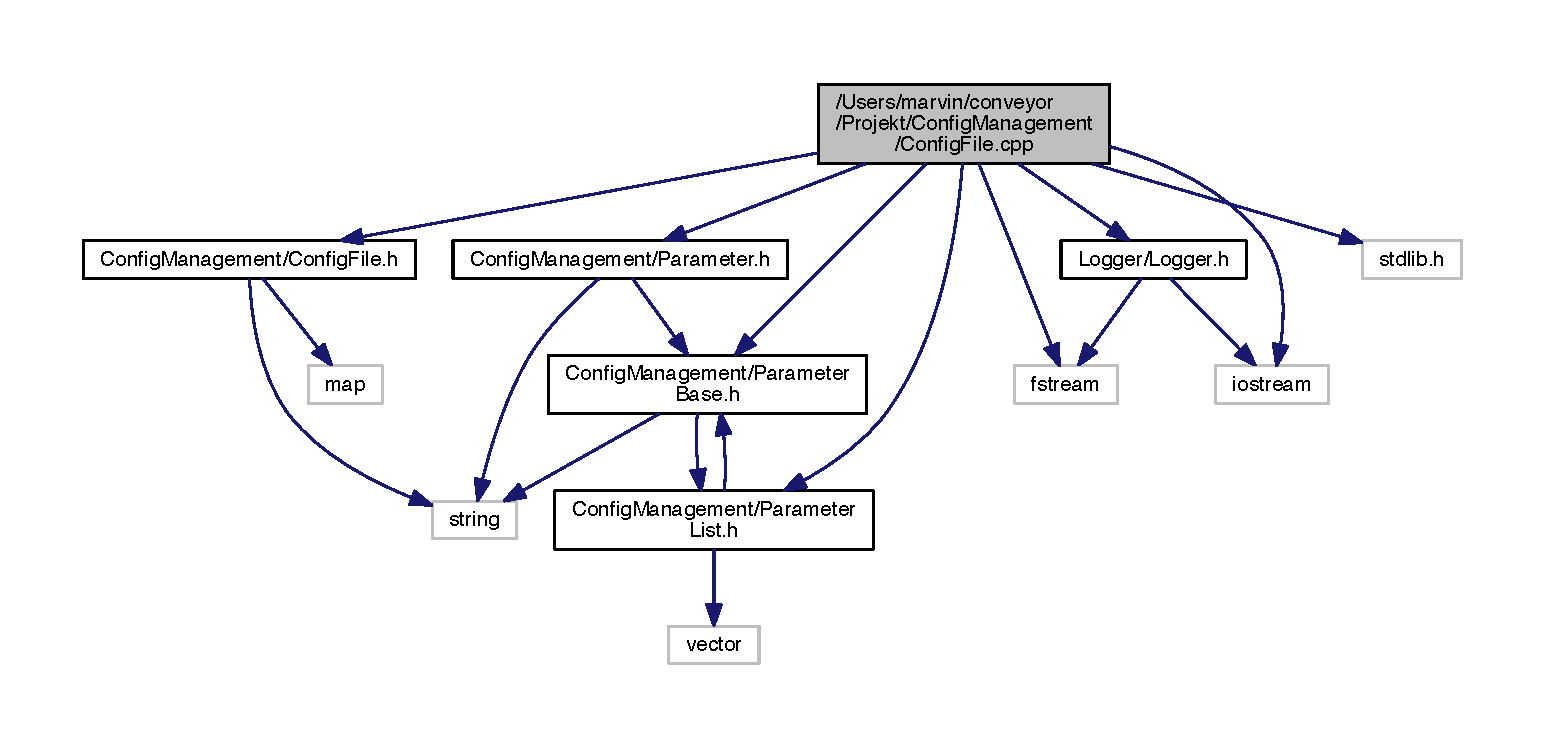
\includegraphics[width=350pt]{_config_file_8cpp__incl}
\end{center}
\end{figure}
\subsection*{Funktionen}
\begin{DoxyCompactItemize}
\item 
std\+::string \hyperlink{_config_file_8cpp_a55f4725e5940f48cd2343de565e9df4e}{trim} (std\+::string const \&source, char const $\ast$delims=\char`\"{} \textbackslash{}\textbackslash{})
\end{DoxyCompactItemize}


\subsection{Dokumentation der Funktionen}
\hypertarget{_config_file_8cpp_a55f4725e5940f48cd2343de565e9df4e}{}\label{_config_file_8cpp_a55f4725e5940f48cd2343de565e9df4e} 
\index{Config\+File.\+cpp@{Config\+File.\+cpp}!trim@{trim}}
\index{trim@{trim}!Config\+File.\+cpp@{Config\+File.\+cpp}}
\subsubsection{\texorpdfstring{trim()}{trim()}}
{\footnotesize\ttfamily std\+::string trim (\begin{DoxyParamCaption}\item[{std\+::string const \&}]{source,  }\item[{char const $\ast$}]{delims = {\ttfamily \char`\"{}~\textbackslash{}t\textbackslash{}r\textbackslash{}n\char`\"{}} }\end{DoxyParamCaption})}


\hypertarget{_config_file_8h}{}\section{Config\+Management/\+Config\+File.h-\/\+Dateireferenz}
\label{_config_file_8h}\index{Config\+Management/\+Config\+File.\+h@{Config\+Management/\+Config\+File.\+h}}
{\ttfamily \#include $<$string$>$}\newline
{\ttfamily \#include $<$map$>$}\newline
{\ttfamily \#include $<$fstream$>$}\newline
{\ttfamily \#include $<$iostream$>$}\newline
{\ttfamily \#include $<$stdlib.\+h$>$}\newline
{\ttfamily \#include \char`\"{}Logger/\+Logger.\+h\char`\"{}}\newline
{\ttfamily \#include \char`\"{}Config\+Management/\+Parameter\+Base.\+h\char`\"{}}\newline
{\ttfamily \#include \char`\"{}Config\+Management/\+Parameter.\+h\char`\"{}}\newline
{\ttfamily \#include \char`\"{}Config\+Management/\+Parameter\+List.\+h\char`\"{}}\newline
Include-\/\+Abhängigkeitsdiagramm für Config\+File.\+h\+:\nopagebreak
\begin{figure}[H]
\begin{center}
\leavevmode
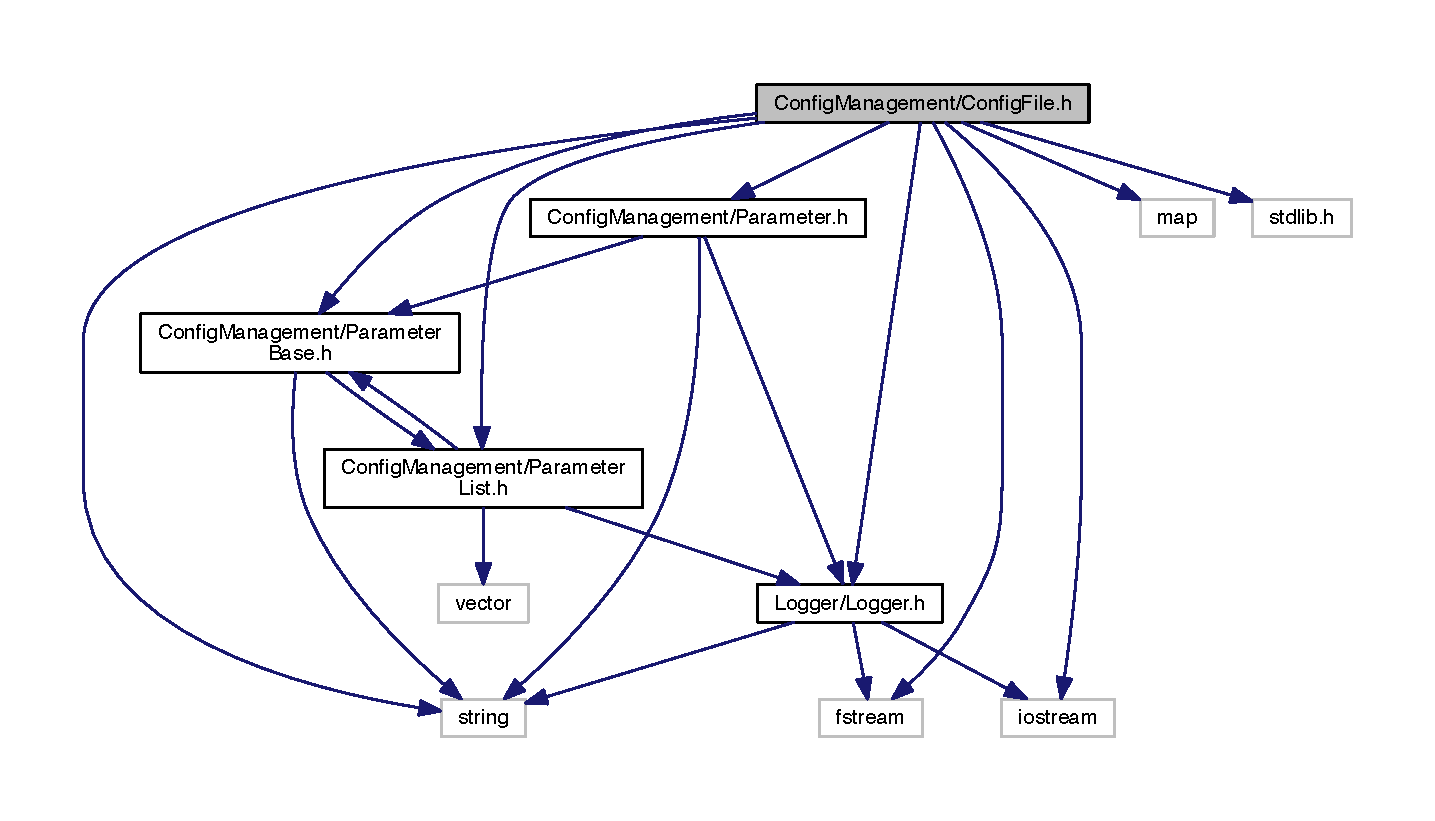
\includegraphics[width=350pt]{_config_file_8h__incl}
\end{center}
\end{figure}
Dieser Graph zeigt, welche Datei direkt oder indirekt diese Datei enthält\+:\nopagebreak
\begin{figure}[H]
\begin{center}
\leavevmode
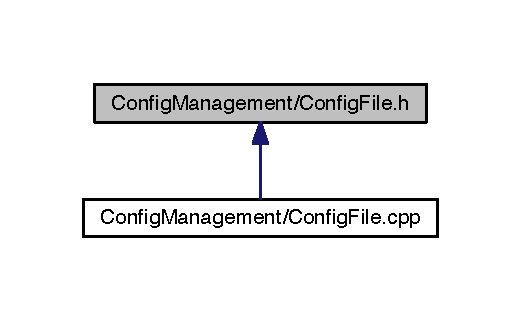
\includegraphics[width=250pt]{_config_file_8h__dep__incl}
\end{center}
\end{figure}
\subsection*{Klassen}
\begin{DoxyCompactItemize}
\item 
class \hyperlink{class_config_file}{Config\+File}
\end{DoxyCompactItemize}


\subsection{Ausführliche Beschreibung}
\hypertarget{_config_updater_thread_8h_DESCRIPTION}{}\subsection{D\+E\+S\+C\+R\+I\+P\+T\+I\+ON}\label{_config_updater_thread_8h_DESCRIPTION}
Eine Klasse um ein Config file zu verwalten. 
\hypertarget{_parameter_8cpp}{}\section{Config\+Management/\+Parameter.cpp-\/\+Dateireferenz}
\label{_parameter_8cpp}\index{Config\+Management/\+Parameter.\+cpp@{Config\+Management/\+Parameter.\+cpp}}
{\ttfamily \#include $<$Config\+Management/\+Parameter.\+h$>$}\newline
{\ttfamily \#include $<$string$>$}\newline
{\ttfamily \#include $<$Logger/\+Logger.\+h$>$}\newline
Include-\/\+Abhängigkeitsdiagramm für Parameter.\+cpp\+:
\nopagebreak
\begin{figure}[H]
\begin{center}
\leavevmode
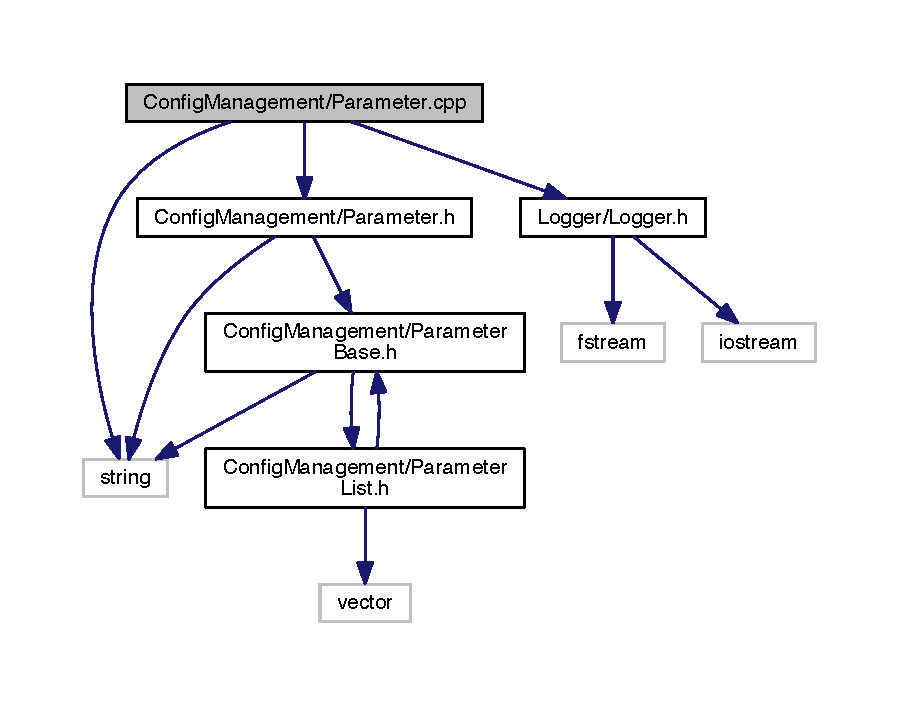
\includegraphics[width=350pt]{_parameter_8cpp__incl}
\end{center}
\end{figure}

\hypertarget{_parameter_8h}{}\section{Config\+Management/\+Parameter.h-\/\+Dateireferenz}
\label{_parameter_8h}\index{Config\+Management/\+Parameter.\+h@{Config\+Management/\+Parameter.\+h}}
{\ttfamily \#include $<$string$>$}\newline
{\ttfamily \#include \char`\"{}Config\+Management/\+Parameter\+Base.\+h\char`\"{}}\newline
{\ttfamily \#include \char`\"{}Logger/\+Logger.\+h\char`\"{}}\newline
Include-\/\+Abhängigkeitsdiagramm für Parameter.\+h\+:\nopagebreak
\begin{figure}[H]
\begin{center}
\leavevmode
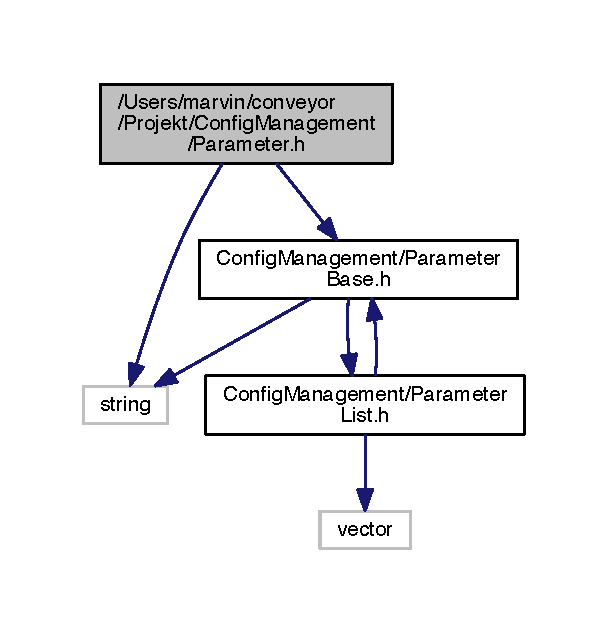
\includegraphics[width=303pt]{_parameter_8h__incl}
\end{center}
\end{figure}
Dieser Graph zeigt, welche Datei direkt oder indirekt diese Datei enthält\+:\nopagebreak
\begin{figure}[H]
\begin{center}
\leavevmode
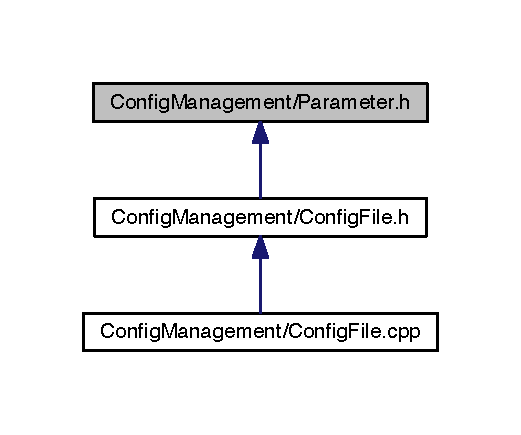
\includegraphics[width=250pt]{_parameter_8h__dep__incl}
\end{center}
\end{figure}
\subsection*{Klassen}
\begin{DoxyCompactItemize}
\item 
class \hyperlink{class_parameter}{Parameter$<$ T $>$}
\end{DoxyCompactItemize}

\hypertarget{_parameter_base_8cpp}{}\section{Config\+Management/\+Parameter\+Base.cpp-\/\+Dateireferenz}
\label{_parameter_base_8cpp}\index{Config\+Management/\+Parameter\+Base.\+cpp@{Config\+Management/\+Parameter\+Base.\+cpp}}
{\ttfamily \#include \char`\"{}Config\+Management/\+Parameter\+Base.\+h\char`\"{}}\newline
Include-\/\+Abhängigkeitsdiagramm für Parameter\+Base.\+cpp\+:\nopagebreak
\begin{figure}[H]
\begin{center}
\leavevmode
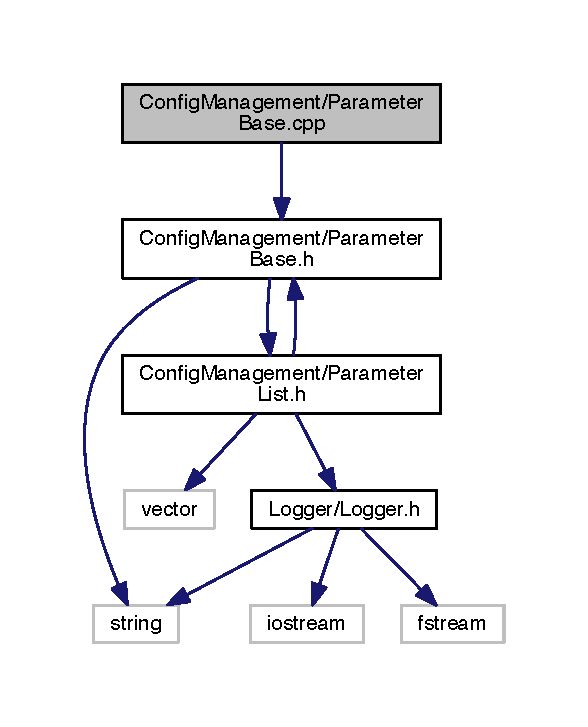
\includegraphics[width=282pt]{_parameter_base_8cpp__incl}
\end{center}
\end{figure}

\hypertarget{_parameter_base_8h}{}\section{Config\+Management/\+Parameter\+Base.h-\/\+Dateireferenz}
\label{_parameter_base_8h}\index{Config\+Management/\+Parameter\+Base.\+h@{Config\+Management/\+Parameter\+Base.\+h}}
{\ttfamily \#include $<$string$>$}\newline
{\ttfamily \#include \char`\"{}Config\+Management/\+Parameter\+List.\+h\char`\"{}}\newline
Include-\/\+Abhängigkeitsdiagramm für Parameter\+Base.\+h\+:
\nopagebreak
\begin{figure}[H]
\begin{center}
\leavevmode
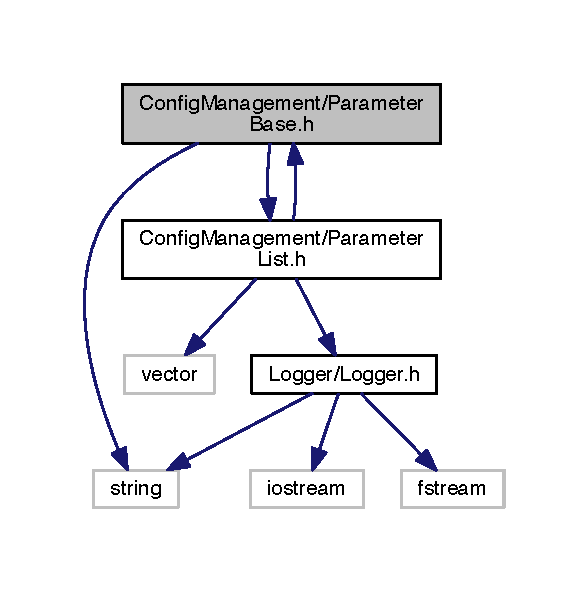
\includegraphics[width=292pt]{_parameter_base_8h__incl}
\end{center}
\end{figure}
Dieser Graph zeigt, welche Datei direkt oder indirekt diese Datei enthält\+:
\nopagebreak
\begin{figure}[H]
\begin{center}
\leavevmode
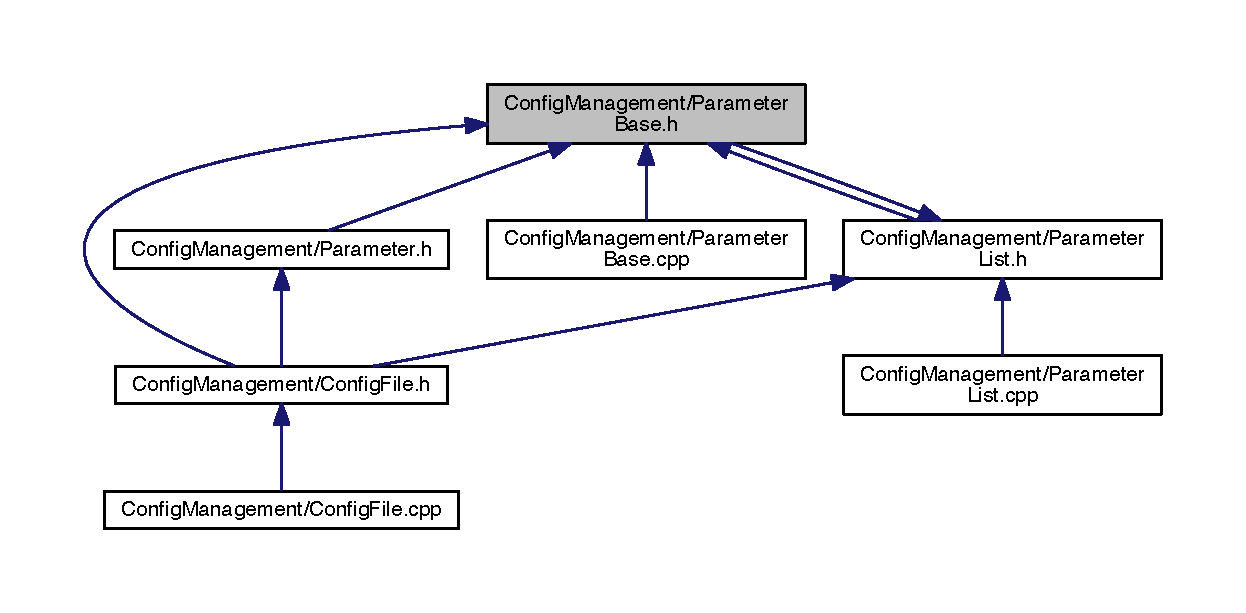
\includegraphics[width=350pt]{_parameter_base_8h__dep__incl}
\end{center}
\end{figure}
\subsection*{Klassen}
\begin{DoxyCompactItemize}
\item 
class \hyperlink{class_parameter_base}{Parameter\+Base}
\end{DoxyCompactItemize}

\hypertarget{_parameter_list_8cpp}{}\section{Config\+Management/\+Parameter\+List.cpp-\/\+Dateireferenz}
\label{_parameter_list_8cpp}\index{Config\+Management/\+Parameter\+List.\+cpp@{Config\+Management/\+Parameter\+List.\+cpp}}
{\ttfamily \#include \char`\"{}Config\+Management/\+Parameter\+List.\+h\char`\"{}}\newline
Include-\/\+Abhängigkeitsdiagramm für Parameter\+List.\+cpp\+:\nopagebreak
\begin{figure}[H]
\begin{center}
\leavevmode
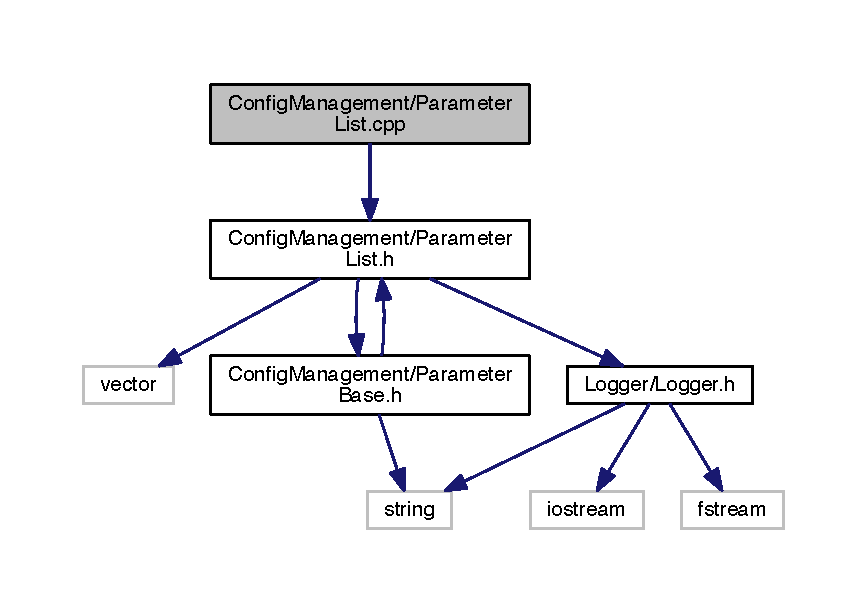
\includegraphics[width=350pt]{_parameter_list_8cpp__incl}
\end{center}
\end{figure}

\hypertarget{_parameter_list_8h}{}\section{Config\+Management/\+Parameter\+List.h-\/\+Dateireferenz}
\label{_parameter_list_8h}\index{Config\+Management/\+Parameter\+List.\+h@{Config\+Management/\+Parameter\+List.\+h}}
{\ttfamily \#include $<$vector$>$}\newline
{\ttfamily \#include \char`\"{}Config\+Management/\+Parameter\+Base.\+h\char`\"{}}\newline
{\ttfamily \#include \char`\"{}Logger/\+Logger.\+h\char`\"{}}\newline
Include-\/\+Abhängigkeitsdiagramm für Parameter\+List.\+h\+:\nopagebreak
\begin{figure}[H]
\begin{center}
\leavevmode
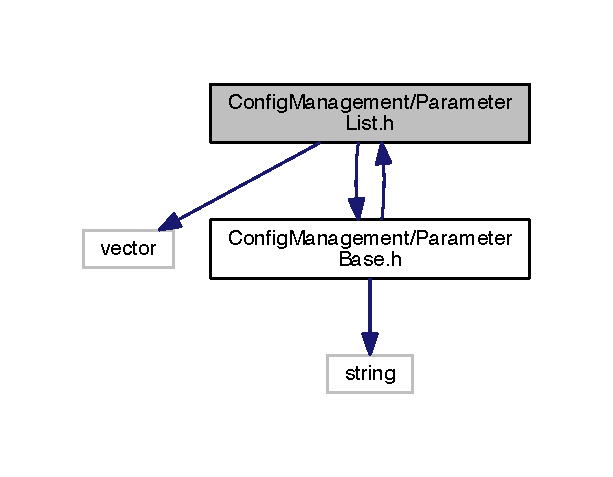
\includegraphics[width=350pt]{_parameter_list_8h__incl}
\end{center}
\end{figure}
Dieser Graph zeigt, welche Datei direkt oder indirekt diese Datei enthält\+:\nopagebreak
\begin{figure}[H]
\begin{center}
\leavevmode
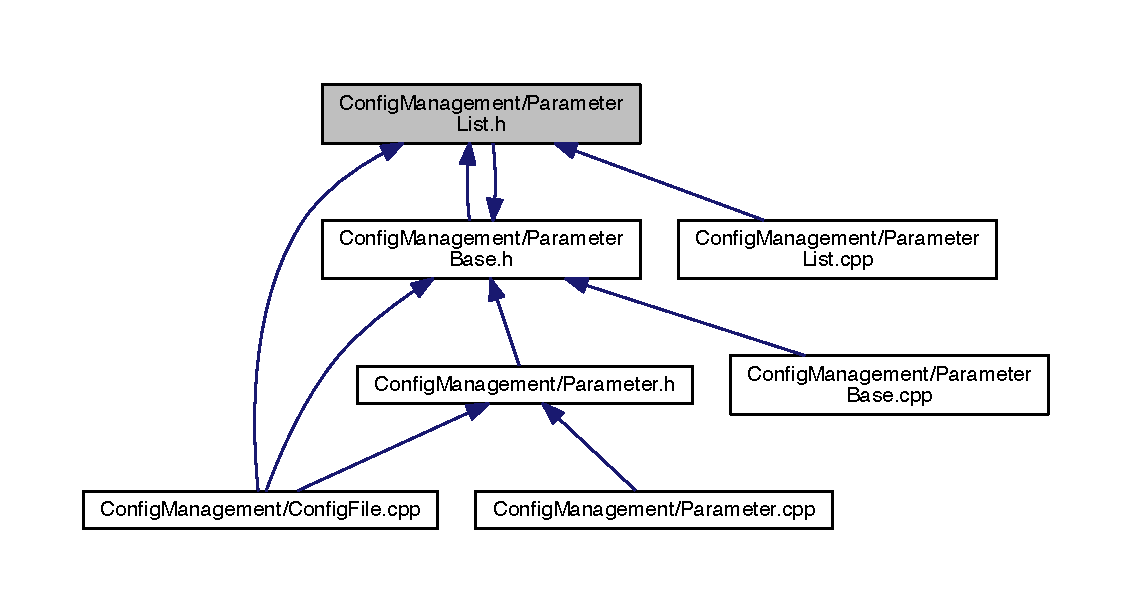
\includegraphics[width=350pt]{_parameter_list_8h__dep__incl}
\end{center}
\end{figure}
\subsection*{Klassen}
\begin{DoxyCompactItemize}
\item 
class \hyperlink{class_parameter_list}{Parameter\+List}
\end{DoxyCompactItemize}


\subsection{Ausführliche Beschreibung}
\hypertarget{_config_updater_thread_8h_DESCRIPTION}{}\subsection{D\+E\+S\+C\+R\+I\+P\+T\+I\+ON}\label{_config_updater_thread_8h_DESCRIPTION}
Eine Klasse um den \hyperlink{class_motor}{Motor} des Foerderbandes an zu sprechen. 
\hypertarget{_conveyor_one_controller_8cpp}{}\section{/\+Users/marvin/conveyor/\+Projekt/\+Controller/\+Conveyor\+One\+Controller.cpp-\/\+Dateireferenz}
\label{_conveyor_one_controller_8cpp}\index{/\+Users/marvin/conveyor/\+Projekt/\+Controller/\+Conveyor\+One\+Controller.\+cpp@{/\+Users/marvin/conveyor/\+Projekt/\+Controller/\+Conveyor\+One\+Controller.\+cpp}}
{\ttfamily \#include $<$Controller/\+Conveyor\+One\+Controller.\+h$>$}\newline
Include-\/\+Abhängigkeitsdiagramm für Conveyor\+One\+Controller.\+cpp\+:
\nopagebreak
\begin{figure}[H]
\begin{center}
\leavevmode
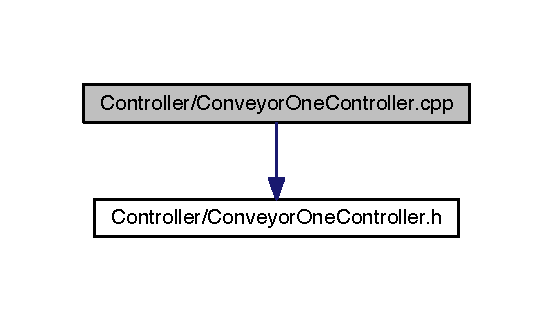
\includegraphics[width=255pt]{_conveyor_one_controller_8cpp__incl}
\end{center}
\end{figure}

\hypertarget{_conveyor_one_controller_8h}{}\section{Controller/\+Conveyor\+One\+Controller.h-\/\+Dateireferenz}
\label{_conveyor_one_controller_8h}\index{Controller/\+Conveyor\+One\+Controller.\+h@{Controller/\+Conveyor\+One\+Controller.\+h}}
Dieser Graph zeigt, welche Datei direkt oder indirekt diese Datei enthält\+:\nopagebreak
\begin{figure}[H]
\begin{center}
\leavevmode
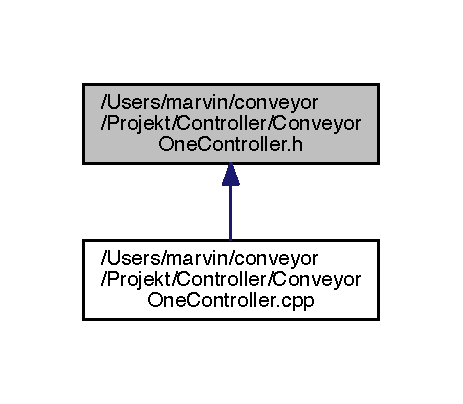
\includegraphics[width=266pt]{_conveyor_one_controller_8h__dep__incl}
\end{center}
\end{figure}
\subsection*{Klassen}
\begin{DoxyCompactItemize}
\item 
class \hyperlink{class_conveyor_one_controller}{Conveyor\+One\+Controller}
\end{DoxyCompactItemize}


\subsection{Ausführliche Beschreibung}
\hypertarget{_config_updater_thread_8h_DESCRIPTION}{}\subsection{D\+E\+S\+C\+R\+I\+P\+T\+I\+ON}\label{_config_updater_thread_8h_DESCRIPTION}
Eine Klasse um den \hyperlink{class_motor}{Motor} des Foerderbandes an zu sprechen. 
\hypertarget{_conveyor_three_controller_8cpp}{}\section{Controller/\+Conveyor\+Three\+Controller.cpp-\/\+Dateireferenz}
\label{_conveyor_three_controller_8cpp}\index{Controller/\+Conveyor\+Three\+Controller.\+cpp@{Controller/\+Conveyor\+Three\+Controller.\+cpp}}
{\ttfamily \#include $<$Controller/\+Conveyor\+Three\+Controller.\+h$>$}\newline
Include-\/\+Abhängigkeitsdiagramm für Conveyor\+Three\+Controller.\+cpp\+:
\nopagebreak
\begin{figure}[H]
\begin{center}
\leavevmode
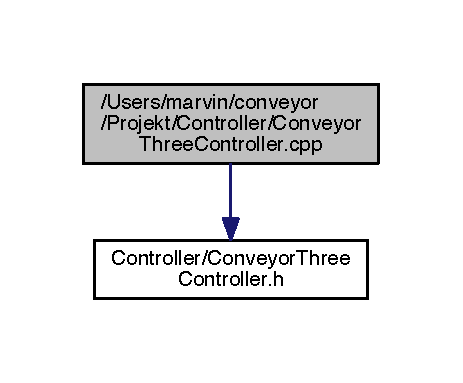
\includegraphics[width=211pt]{_conveyor_three_controller_8cpp__incl}
\end{center}
\end{figure}

\hypertarget{_conveyor_three_controller_8h}{}\section{Controller/\+Conveyor\+Three\+Controller.h-\/\+Dateireferenz}
\label{_conveyor_three_controller_8h}\index{Controller/\+Conveyor\+Three\+Controller.\+h@{Controller/\+Conveyor\+Three\+Controller.\+h}}
Dieser Graph zeigt, welche Datei direkt oder indirekt diese Datei enthält\+:\nopagebreak
\begin{figure}[H]
\begin{center}
\leavevmode
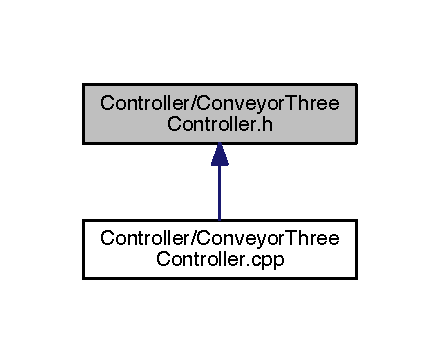
\includegraphics[width=211pt]{_conveyor_three_controller_8h__dep__incl}
\end{center}
\end{figure}
\subsection*{Klassen}
\begin{DoxyCompactItemize}
\item 
class \hyperlink{class_conveyor_three_controller}{Conveyor\+Three\+Controller}
\end{DoxyCompactItemize}


\subsection{Ausführliche Beschreibung}
\hypertarget{_config_updater_thread_8h_DESCRIPTION}{}\subsection{D\+E\+S\+C\+R\+I\+P\+T\+I\+ON}\label{_config_updater_thread_8h_DESCRIPTION}
Eine Klasse um den \hyperlink{class_motor}{Motor} des Foerderbandes an zu sprechen. 
\hypertarget{_conveyor_two_controller_8cpp}{}\section{Controller/\+Conveyor\+Two\+Controller.cpp-\/\+Dateireferenz}
\label{_conveyor_two_controller_8cpp}\index{Controller/\+Conveyor\+Two\+Controller.\+cpp@{Controller/\+Conveyor\+Two\+Controller.\+cpp}}
{\ttfamily \#include $<$Controller/\+Conveyor\+Two\+Controller.\+h$>$}\newline
Include-\/\+Abhängigkeitsdiagramm für Conveyor\+Two\+Controller.\+cpp\+:\nopagebreak
\begin{figure}[H]
\begin{center}
\leavevmode
\includegraphics[width=265pt]{_conveyor_two_controller_8cpp__incl}
\end{center}
\end{figure}

\hypertarget{_conveyor_two_controller_8h}{}\section{Controller/\+Conveyor\+Two\+Controller.h-\/\+Dateireferenz}
\label{_conveyor_two_controller_8h}\index{Controller/\+Conveyor\+Two\+Controller.\+h@{Controller/\+Conveyor\+Two\+Controller.\+h}}
Dieser Graph zeigt, welche Datei direkt oder indirekt diese Datei enthält\+:
\nopagebreak
\begin{figure}[H]
\begin{center}
\leavevmode
\includegraphics[width=265pt]{_conveyor_two_controller_8h__dep__incl}
\end{center}
\end{figure}
\subsection*{Klassen}
\begin{DoxyCompactItemize}
\item 
class \hyperlink{class_conveyor_two_controller}{Conveyor\+Two\+Controller}
\end{DoxyCompactItemize}

\hypertarget{conveyor_8cc}{}\section{conveyor.\+cc-\/\+Dateireferenz}
\label{conveyor_8cc}\index{conveyor.\+cc@{conveyor.\+cc}}
{\ttfamily \#include $<$cstdlib$>$}\newline
{\ttfamily \#include $<$iostream$>$}\newline
{\ttfamily \#include \char`\"{}Hal/\+Hal\+Builder.\+h\char`\"{}}\newline
{\ttfamily \#include \char`\"{}Thread/\+Conveyor\+Thread.\+h\char`\"{}}\newline
Include-\/\+Abhängigkeitsdiagramm für conveyor.\+cc\+:
\nopagebreak
\begin{figure}[H]
\begin{center}
\leavevmode
\includegraphics[width=350pt]{conveyor_8cc__incl}
\end{center}
\end{figure}
\subsection*{Funktionen}
\begin{DoxyCompactItemize}
\item 
int \hyperlink{conveyor_8cc_a0ddf1224851353fc92bfbff6f499fa97}{main} (int argc, char $\ast$argv\mbox{[}$\,$\mbox{]})
\end{DoxyCompactItemize}


\subsection{Dokumentation der Funktionen}
\hypertarget{conveyor_8cc_a0ddf1224851353fc92bfbff6f499fa97}{}\label{conveyor_8cc_a0ddf1224851353fc92bfbff6f499fa97} 
\index{conveyor.\+cc@{conveyor.\+cc}!main@{main}}
\index{main@{main}!conveyor.\+cc@{conveyor.\+cc}}
\subsubsection{\texorpdfstring{main()}{main()}}
{\footnotesize\ttfamily int main (\begin{DoxyParamCaption}\item[{int}]{argc,  }\item[{char $\ast$}]{argv\mbox{[}$\,$\mbox{]} }\end{DoxyParamCaption})}


\hypertarget{_serial_message_8cpp}{}\section{Entity/\+Serial\+Message.cpp-\/\+Dateireferenz}
\label{_serial_message_8cpp}\index{Entity/\+Serial\+Message.\+cpp@{Entity/\+Serial\+Message.\+cpp}}
{\ttfamily \#include $<$Entity/\+Serial\+Message.\+h$>$}\newline
Include-\/\+Abhängigkeitsdiagramm für Serial\+Message.\+cpp\+:
\nopagebreak
\begin{figure}[H]
\begin{center}
\leavevmode
\includegraphics[width=209pt]{_serial_message_8cpp__incl}
\end{center}
\end{figure}

\hypertarget{_serial_message_8h}{}\section{/\+Users/marvin/conveyor/\+Projekt/\+Entity/\+Serial\+Message.h-\/\+Dateireferenz}
\label{_serial_message_8h}\index{/\+Users/marvin/conveyor/\+Projekt/\+Entity/\+Serial\+Message.\+h@{/\+Users/marvin/conveyor/\+Projekt/\+Entity/\+Serial\+Message.\+h}}
Dieser Graph zeigt, welche Datei direkt oder indirekt diese Datei enthält\+:
\nopagebreak
\begin{figure}[H]
\begin{center}
\leavevmode
\includegraphics[width=246pt]{_serial_message_8h__dep__incl}
\end{center}
\end{figure}
\subsection*{Klassen}
\begin{DoxyCompactItemize}
\item 
class \hyperlink{class_serial_message}{Serial\+Message}
\end{DoxyCompactItemize}

\hypertarget{_f_s_m_2_context_8cpp}{}\section{F\+S\+M/\+Context.cpp-\/\+Dateireferenz}
\label{_f_s_m_2_context_8cpp}\index{F\+S\+M/\+Context.\+cpp@{F\+S\+M/\+Context.\+cpp}}
{\ttfamily \#include \char`\"{}Context.\+h\char`\"{}}\newline
Include-\/\+Abhängigkeitsdiagramm für Context.\+cpp\+:
\nopagebreak
\begin{figure}[H]
\begin{center}
\leavevmode
\includegraphics[width=350pt]{_f_s_m_2_context_8cpp__incl}
\end{center}
\end{figure}

\hypertarget{test_2_h_a_l_2_sensorik_2_context_8cpp}{}\section{test/\+H\+A\+L/\+Sensorik/\+Context.cpp-\/\+Dateireferenz}
\label{test_2_h_a_l_2_sensorik_2_context_8cpp}\index{test/\+H\+A\+L/\+Sensorik/\+Context.\+cpp@{test/\+H\+A\+L/\+Sensorik/\+Context.\+cpp}}
{\ttfamily \#include \char`\"{}Context.\+h\char`\"{}}\newline
Include-\/\+Abhängigkeitsdiagramm für Context.\+cpp\+:
\nopagebreak
\begin{figure}[H]
\begin{center}
\leavevmode
\includegraphics[width=350pt]{test_2_h_a_l_2_sensorik_2_context_8cpp__incl}
\end{center}
\end{figure}

\hypertarget{_f_s_m_2_context_8h}{}\section{F\+S\+M/\+Context.h-\/\+Dateireferenz}
\label{_f_s_m_2_context_8h}\index{F\+S\+M/\+Context.\+h@{F\+S\+M/\+Context.\+h}}
{\ttfamily \#include $<$iostream$>$}\newline
{\ttfamily \#include \char`\"{}Logger/\+Logger.\+h\char`\"{}}\newline
{\ttfamily \#include \char`\"{}Hal/\+Hal\+Builder.\+h\char`\"{}}\newline
Include-\/\+Abhängigkeitsdiagramm für Context.\+h\+:
\nopagebreak
\begin{figure}[H]
\begin{center}
\leavevmode
\includegraphics[width=350pt]{_f_s_m_2_context_8h__incl}
\end{center}
\end{figure}
Dieser Graph zeigt, welche Datei direkt oder indirekt diese Datei enthält\+:
\nopagebreak
\begin{figure}[H]
\begin{center}
\leavevmode
\includegraphics[width=350pt]{_f_s_m_2_context_8h__dep__incl}
\end{center}
\end{figure}
\subsection*{Klassen}
\begin{DoxyCompactItemize}
\item 
class \hyperlink{class_context}{Context}
\end{DoxyCompactItemize}
\subsection*{Variablen}
\begin{DoxyCompactItemize}
\item 
\hyperlink{class_hal_builder}{Hal\+Builder} \hyperlink{_f_s_m_2_context_8h_a150c49d0f49ad0bbff3e8e7c1e32aef5}{hb}
\end{DoxyCompactItemize}


\subsection{Ausführliche Beschreibung}
\hypertarget{_config_updater_thread_8h_DESCRIPTION}{}\subsection{D\+E\+S\+C\+R\+I\+P\+T\+I\+ON}\label{_config_updater_thread_8h_DESCRIPTION}
Eine Klasse um den \hyperlink{class_motor}{Motor} des Foerderbandes an zu sprechen. 

\subsection{Variablen-\/\+Dokumentation}
\hypertarget{_f_s_m_2_context_8h_a150c49d0f49ad0bbff3e8e7c1e32aef5}{}\label{_f_s_m_2_context_8h_a150c49d0f49ad0bbff3e8e7c1e32aef5} 
\index{F\+S\+M/\+Context.\+h@{F\+S\+M/\+Context.\+h}!hb@{hb}}
\index{hb@{hb}!F\+S\+M/\+Context.\+h@{F\+S\+M/\+Context.\+h}}
\subsubsection{\texorpdfstring{hb}{hb}}
{\footnotesize\ttfamily \hyperlink{class_hal_builder}{Hal\+Builder} hb}


\hypertarget{test_2_h_a_l_2_sensorik_2_context_8h}{}\section{test/\+H\+A\+L/\+Sensorik/\+Context.h-\/\+Dateireferenz}
\label{test_2_h_a_l_2_sensorik_2_context_8h}\index{test/\+H\+A\+L/\+Sensorik/\+Context.\+h@{test/\+H\+A\+L/\+Sensorik/\+Context.\+h}}
{\ttfamily \#include $<$iostream$>$}\newline
{\ttfamily \#include \char`\"{}Logger/\+Logger.\+h\char`\"{}}\newline
{\ttfamily \#include \char`\"{}Hal/\+Hal\+Builder.\+h\char`\"{}}\newline
Include-\/\+Abhängigkeitsdiagramm für Context.\+h\+:\nopagebreak
\begin{figure}[H]
\begin{center}
\leavevmode
\includegraphics[width=350pt]{test_2_h_a_l_2_sensorik_2_context_8h__incl}
\end{center}
\end{figure}
Dieser Graph zeigt, welche Datei direkt oder indirekt diese Datei enthält\+:\nopagebreak
\begin{figure}[H]
\begin{center}
\leavevmode
\includegraphics[width=232pt]{test_2_h_a_l_2_sensorik_2_context_8h__dep__incl}
\end{center}
\end{figure}
\subsection*{Klassen}
\begin{DoxyCompactItemize}
\item 
class \hyperlink{class_context}{Context}
\end{DoxyCompactItemize}
\subsection*{Variablen}
\begin{DoxyCompactItemize}
\item 
\hyperlink{class_hal_builder}{Hal\+Builder} \hyperlink{test_2_h_a_l_2_sensorik_2_context_8h_a150c49d0f49ad0bbff3e8e7c1e32aef5}{hb}
\begin{DoxyCompactList}\small\item\em Der \hyperlink{class_hal_builder}{Hal\+Builder} um sicher und zentral auf die \hyperlink{class_hardware}{Hardware} zuzugreifen. \end{DoxyCompactList}\end{DoxyCompactItemize}


\subsection{Ausführliche Beschreibung}
\hypertarget{_config_updater_thread_8h_DESCRIPTION}{}\subsection{D\+E\+S\+C\+R\+I\+P\+T\+I\+ON}\label{_config_updater_thread_8h_DESCRIPTION}
Eine Klasse um den \hyperlink{class_motor}{Motor} des Foerderbandes an zu sprechen. 

\subsection{Variablen-\/\+Dokumentation}
\hypertarget{test_2_h_a_l_2_sensorik_2_context_8h_a150c49d0f49ad0bbff3e8e7c1e32aef5}{}\label{test_2_h_a_l_2_sensorik_2_context_8h_a150c49d0f49ad0bbff3e8e7c1e32aef5} 
\index{test/\+H\+A\+L/\+Sensorik/\+Context.\+h@{test/\+H\+A\+L/\+Sensorik/\+Context.\+h}!hb@{hb}}
\index{hb@{hb}!test/\+H\+A\+L/\+Sensorik/\+Context.\+h@{test/\+H\+A\+L/\+Sensorik/\+Context.\+h}}
\subsubsection{\texorpdfstring{hb}{hb}}
{\footnotesize\ttfamily \hyperlink{class_hal_builder}{Hal\+Builder} hb}



Der \hyperlink{class_hal_builder}{Hal\+Builder} um sicher und zentral auf die \hyperlink{class_hardware}{Hardware} zuzugreifen. 


\hypertarget{_adapter_8cpp}{}\section{/\+Users/marvin/conveyor/\+Projekt/\+Hal/\+Adapter.cpp-\/\+Dateireferenz}
\label{_adapter_8cpp}\index{/\+Users/marvin/conveyor/\+Projekt/\+Hal/\+Adapter.\+cpp@{/\+Users/marvin/conveyor/\+Projekt/\+Hal/\+Adapter.\+cpp}}
{\ttfamily \#include $<$Hal/\+Adapter.\+h$>$}\newline
Include-\/\+Abhängigkeitsdiagramm für Adapter.\+cpp\+:
\nopagebreak
\begin{figure}[H]
\begin{center}
\leavevmode
\includegraphics[width=301pt]{_adapter_8cpp__incl}
\end{center}
\end{figure}

\hypertarget{_adapter_8h}{}\section{Hal/\+Adapter.h-\/\+Dateireferenz}
\label{_adapter_8h}\index{Hal/\+Adapter.\+h@{Hal/\+Adapter.\+h}}
{\ttfamily \#include $<$stdint.\+h$>$}\newline
{\ttfamily \#include $<$Hal/\+Mutexo.\+h$>$}\newline
{\ttfamily \#include $<$hw/inout.\+h$>$}\newline
Include-\/\+Abhängigkeitsdiagramm für Adapter.\+h\+:\nopagebreak
\begin{figure}[H]
\begin{center}
\leavevmode
\includegraphics[width=301pt]{_adapter_8h__incl}
\end{center}
\end{figure}
Dieser Graph zeigt, welche Datei direkt oder indirekt diese Datei enthält\+:
\nopagebreak
\begin{figure}[H]
\begin{center}
\leavevmode
\includegraphics[width=350pt]{_adapter_8h__dep__incl}
\end{center}
\end{figure}
\subsection*{Klassen}
\begin{DoxyCompactItemize}
\item 
class \hyperlink{class_adapter}{Adapter}
\end{DoxyCompactItemize}


\subsection{Ausführliche Beschreibung}
\hypertarget{_config_updater_thread_8h_DESCRIPTION}{}\subsection{D\+E\+S\+C\+R\+I\+P\+T\+I\+ON}\label{_config_updater_thread_8h_DESCRIPTION}
Eine Klasse um den \hyperlink{class_adapter}{Adapter(\+Ports)} zugriff zu Managen. 
\hypertarget{_altimetry_8cpp}{}\section{Hal/\+Altimetry.cpp-\/\+Dateireferenz}
\label{_altimetry_8cpp}\index{Hal/\+Altimetry.\+cpp@{Hal/\+Altimetry.\+cpp}}
{\ttfamily \#include \char`\"{}Altimetry.\+h\char`\"{}}\newline
Include-\/\+Abhängigkeitsdiagramm für Altimetry.\+cpp\+:
\nopagebreak
\begin{figure}[H]
\begin{center}
\leavevmode
\includegraphics[width=350pt]{_altimetry_8cpp__incl}
\end{center}
\end{figure}

\hypertarget{_altimetry_8h}{}\section{Hal/\+Altimetry.h-\/\+Dateireferenz}
\label{_altimetry_8h}\index{Hal/\+Altimetry.\+h@{Hal/\+Altimetry.\+h}}
{\ttfamily \#include $<$hw/inout.\+h$>$}\newline
{\ttfamily \#include $<$stdint.\+h$>$}\newline
{\ttfamily \#include \char`\"{}Logger/\+Logger.\+h\char`\"{}}\newline
{\ttfamily \#include \char`\"{}Hal/\+Adapter.\+h\char`\"{}}\newline
Include-\/\+Abhängigkeitsdiagramm für Altimetry.\+h\+:\nopagebreak
\begin{figure}[H]
\begin{center}
\leavevmode
\includegraphics[width=350pt]{_altimetry_8h__incl}
\end{center}
\end{figure}
Dieser Graph zeigt, welche Datei direkt oder indirekt diese Datei enthält\+:
\nopagebreak
\begin{figure}[H]
\begin{center}
\leavevmode
\includegraphics[width=350pt]{_altimetry_8h__dep__incl}
\end{center}
\end{figure}
\subsection*{Klassen}
\begin{DoxyCompactItemize}
\item 
class \hyperlink{class_altimetry}{Altimetry}
\end{DoxyCompactItemize}
\subsection*{Makrodefinitionen}
\begin{DoxyCompactItemize}
\item 
\#define \hyperlink{_altimetry_8h_af5f248978814b43f265459187d85217f}{A\+C\+T\+I\+V\+A\+T\+E\+\_\+\+A\+D\+C\+\_\+\+IN}~0b10000100
\begin{DoxyCompactList}\small\item\em Befehl um die Interrupts bei dem A\+DC zu aktivieren. \end{DoxyCompactList}\item 
\#define \hyperlink{_altimetry_8h_a66517a19dec0aa83aeda71c205a4dd2c}{A\+D\+C\+\_\+\+I\+N\+\_\+\+O\+F\+F\+S\+ET}~0x01
\begin{DoxyCompactList}\small\item\em Offset zu dem A\+DC Config Register. \end{DoxyCompactList}\end{DoxyCompactItemize}


\subsection{Ausführliche Beschreibung}
\hypertarget{_config_updater_thread_8h_DESCRIPTION}{}\subsection{D\+E\+S\+C\+R\+I\+P\+T\+I\+ON}\label{_config_updater_thread_8h_DESCRIPTION}
Eine Klasse um die Ampel des Foerderbandes zu Steuern. 

\subsection{Makro-\/\+Dokumentation}
\hypertarget{_altimetry_8h_af5f248978814b43f265459187d85217f}{}\label{_altimetry_8h_af5f248978814b43f265459187d85217f} 
\index{Altimetry.\+h@{Altimetry.\+h}!A\+C\+T\+I\+V\+A\+T\+E\+\_\+\+A\+D\+C\+\_\+\+IN@{A\+C\+T\+I\+V\+A\+T\+E\+\_\+\+A\+D\+C\+\_\+\+IN}}
\index{A\+C\+T\+I\+V\+A\+T\+E\+\_\+\+A\+D\+C\+\_\+\+IN@{A\+C\+T\+I\+V\+A\+T\+E\+\_\+\+A\+D\+C\+\_\+\+IN}!Altimetry.\+h@{Altimetry.\+h}}
\subsubsection{\texorpdfstring{A\+C\+T\+I\+V\+A\+T\+E\+\_\+\+A\+D\+C\+\_\+\+IN}{ACTIVATE\_ADC\_IN}}
{\footnotesize\ttfamily \#define A\+C\+T\+I\+V\+A\+T\+E\+\_\+\+A\+D\+C\+\_\+\+IN~0b10000100}



Befehl um die Interrupts bei dem A\+DC zu aktivieren. 

\hypertarget{_altimetry_8h_a66517a19dec0aa83aeda71c205a4dd2c}{}\label{_altimetry_8h_a66517a19dec0aa83aeda71c205a4dd2c} 
\index{Altimetry.\+h@{Altimetry.\+h}!A\+D\+C\+\_\+\+I\+N\+\_\+\+O\+F\+F\+S\+ET@{A\+D\+C\+\_\+\+I\+N\+\_\+\+O\+F\+F\+S\+ET}}
\index{A\+D\+C\+\_\+\+I\+N\+\_\+\+O\+F\+F\+S\+ET@{A\+D\+C\+\_\+\+I\+N\+\_\+\+O\+F\+F\+S\+ET}!Altimetry.\+h@{Altimetry.\+h}}
\subsubsection{\texorpdfstring{A\+D\+C\+\_\+\+I\+N\+\_\+\+O\+F\+F\+S\+ET}{ADC\_IN\_OFFSET}}
{\footnotesize\ttfamily \#define A\+D\+C\+\_\+\+I\+N\+\_\+\+O\+F\+F\+S\+ET~0x01}



Offset zu dem A\+DC Config Register. 


\hypertarget{_hal_builder_8cpp}{}\section{Hal/\+Hal\+Builder.cpp-\/\+Dateireferenz}
\label{_hal_builder_8cpp}\index{Hal/\+Hal\+Builder.\+cpp@{Hal/\+Hal\+Builder.\+cpp}}
{\ttfamily \#include $<$Hal\+Builder.\+h$>$}\newline
Include-\/\+Abhängigkeitsdiagramm für Hal\+Builder.\+cpp\+:
\nopagebreak
\begin{figure}[H]
\begin{center}
\leavevmode
\includegraphics[width=350pt]{_hal_builder_8cpp__incl}
\end{center}
\end{figure}

\hypertarget{_hal_builder_8h}{}\section{Hal/\+Hal\+Builder.h-\/\+Dateireferenz}
\label{_hal_builder_8h}\index{Hal/\+Hal\+Builder.\+h@{Hal/\+Hal\+Builder.\+h}}
{\ttfamily \#include \char`\"{}Hal/\+Adapter.\+h\char`\"{}}\newline
{\ttfamily \#include \char`\"{}Hal/\+Hardware.\+h\char`\"{}}\newline
{\ttfamily \#include \char`\"{}Hal/\+Motor.\+h\char`\"{}}\newline
{\ttfamily \#include \char`\"{}Hal/\+Human\+Machine\+Interface.\+h\char`\"{}}\newline
{\ttfamily \#include \char`\"{}Hal/\+Measuring\+Tool.\+h\char`\"{}}\newline
{\ttfamily \#include \char`\"{}Hal/\+Traffic\+Light.\+h\char`\"{}}\newline
{\ttfamily \#include \char`\"{}Hal/\+Mutexo.\+h\char`\"{}}\newline
Include-\/\+Abhängigkeitsdiagramm für Hal\+Builder.\+h\+:
\nopagebreak
\begin{figure}[H]
\begin{center}
\leavevmode
\includegraphics[width=350pt]{_hal_builder_8h__incl}
\end{center}
\end{figure}
Dieser Graph zeigt, welche Datei direkt oder indirekt diese Datei enthält\+:
\nopagebreak
\begin{figure}[H]
\begin{center}
\leavevmode
\includegraphics[width=350pt]{_hal_builder_8h__dep__incl}
\end{center}
\end{figure}
\subsection*{Klassen}
\begin{DoxyCompactItemize}
\item 
class \hyperlink{class_hal_builder}{Hal\+Builder}
\end{DoxyCompactItemize}
\subsection*{Makrodefinitionen}
\begin{DoxyCompactItemize}
\item 
\#define \hyperlink{_hal_builder_8h_ad736ed16a7169899ab9d6025889d5058}{B\+A\+S\+E\+A\+D\+R\+E\+S\+S\+\_\+A}~0x300
\item 
\#define \hyperlink{_hal_builder_8h_acc5f003906c7554a5b88497f199cb389}{B\+A\+S\+E\+A\+D\+R\+E\+S\+S\+\_\+B}~0x301
\item 
\#define \hyperlink{_hal_builder_8h_acc425eae8132245edae734f9d29bef3c}{B\+A\+S\+E\+A\+D\+R\+E\+S\+S\+\_\+C}~0x302
\item 
\#define \hyperlink{_hal_builder_8h_a1e248eb700ba9d3d9a2e1319566a4984}{B\+A\+S\+E\+A\+D\+R\+E\+S\+S\+\_\+D}~0x320
\item 
\#define \hyperlink{_hal_builder_8h_aaa66171c75a1dd400cd567543e42550a}{C\+O\+N\+T\+R\+O\+L\+\_\+\+A\+D\+D\+R\+E\+S\+S\+\_\+0}~0x303
\item 
\#define \hyperlink{_hal_builder_8h_a3df51240b700f60df3ff9842ac7b41a3}{C\+O\+N\+T\+R\+O\+L\+\_\+\+B\+I\+T\+M\+A\+SK}~0x8A
\end{DoxyCompactItemize}


\subsection{Ausführliche Beschreibung}
\hypertarget{_config_updater_thread_8h_DESCRIPTION}{}\subsection{D\+E\+S\+C\+R\+I\+P\+T\+I\+ON}\label{_config_updater_thread_8h_DESCRIPTION}
Eine Klasse um den \hyperlink{class_motor}{Motor} des Foerderbandes an zu sprechen. 

\subsection{Makro-\/\+Dokumentation}
\hypertarget{_hal_builder_8h_ad736ed16a7169899ab9d6025889d5058}{}\label{_hal_builder_8h_ad736ed16a7169899ab9d6025889d5058} 
\index{Hal\+Builder.\+h@{Hal\+Builder.\+h}!B\+A\+S\+E\+A\+D\+R\+E\+S\+S\+\_\+A@{B\+A\+S\+E\+A\+D\+R\+E\+S\+S\+\_\+A}}
\index{B\+A\+S\+E\+A\+D\+R\+E\+S\+S\+\_\+A@{B\+A\+S\+E\+A\+D\+R\+E\+S\+S\+\_\+A}!Hal\+Builder.\+h@{Hal\+Builder.\+h}}
\subsubsection{\texorpdfstring{B\+A\+S\+E\+A\+D\+R\+E\+S\+S\+\_\+A}{BASEADRESS\_A}}
{\footnotesize\ttfamily \#define B\+A\+S\+E\+A\+D\+R\+E\+S\+S\+\_\+A~0x300}

\hypertarget{_hal_builder_8h_acc5f003906c7554a5b88497f199cb389}{}\label{_hal_builder_8h_acc5f003906c7554a5b88497f199cb389} 
\index{Hal\+Builder.\+h@{Hal\+Builder.\+h}!B\+A\+S\+E\+A\+D\+R\+E\+S\+S\+\_\+B@{B\+A\+S\+E\+A\+D\+R\+E\+S\+S\+\_\+B}}
\index{B\+A\+S\+E\+A\+D\+R\+E\+S\+S\+\_\+B@{B\+A\+S\+E\+A\+D\+R\+E\+S\+S\+\_\+B}!Hal\+Builder.\+h@{Hal\+Builder.\+h}}
\subsubsection{\texorpdfstring{B\+A\+S\+E\+A\+D\+R\+E\+S\+S\+\_\+B}{BASEADRESS\_B}}
{\footnotesize\ttfamily \#define B\+A\+S\+E\+A\+D\+R\+E\+S\+S\+\_\+B~0x301}

\hypertarget{_hal_builder_8h_acc425eae8132245edae734f9d29bef3c}{}\label{_hal_builder_8h_acc425eae8132245edae734f9d29bef3c} 
\index{Hal\+Builder.\+h@{Hal\+Builder.\+h}!B\+A\+S\+E\+A\+D\+R\+E\+S\+S\+\_\+C@{B\+A\+S\+E\+A\+D\+R\+E\+S\+S\+\_\+C}}
\index{B\+A\+S\+E\+A\+D\+R\+E\+S\+S\+\_\+C@{B\+A\+S\+E\+A\+D\+R\+E\+S\+S\+\_\+C}!Hal\+Builder.\+h@{Hal\+Builder.\+h}}
\subsubsection{\texorpdfstring{B\+A\+S\+E\+A\+D\+R\+E\+S\+S\+\_\+C}{BASEADRESS\_C}}
{\footnotesize\ttfamily \#define B\+A\+S\+E\+A\+D\+R\+E\+S\+S\+\_\+C~0x302}

\hypertarget{_hal_builder_8h_a1e248eb700ba9d3d9a2e1319566a4984}{}\label{_hal_builder_8h_a1e248eb700ba9d3d9a2e1319566a4984} 
\index{Hal\+Builder.\+h@{Hal\+Builder.\+h}!B\+A\+S\+E\+A\+D\+R\+E\+S\+S\+\_\+D@{B\+A\+S\+E\+A\+D\+R\+E\+S\+S\+\_\+D}}
\index{B\+A\+S\+E\+A\+D\+R\+E\+S\+S\+\_\+D@{B\+A\+S\+E\+A\+D\+R\+E\+S\+S\+\_\+D}!Hal\+Builder.\+h@{Hal\+Builder.\+h}}
\subsubsection{\texorpdfstring{B\+A\+S\+E\+A\+D\+R\+E\+S\+S\+\_\+D}{BASEADRESS\_D}}
{\footnotesize\ttfamily \#define B\+A\+S\+E\+A\+D\+R\+E\+S\+S\+\_\+D~0x320}

\hypertarget{_hal_builder_8h_aaa66171c75a1dd400cd567543e42550a}{}\label{_hal_builder_8h_aaa66171c75a1dd400cd567543e42550a} 
\index{Hal\+Builder.\+h@{Hal\+Builder.\+h}!C\+O\+N\+T\+R\+O\+L\+\_\+\+A\+D\+D\+R\+E\+S\+S\+\_\+0@{C\+O\+N\+T\+R\+O\+L\+\_\+\+A\+D\+D\+R\+E\+S\+S\+\_\+0}}
\index{C\+O\+N\+T\+R\+O\+L\+\_\+\+A\+D\+D\+R\+E\+S\+S\+\_\+0@{C\+O\+N\+T\+R\+O\+L\+\_\+\+A\+D\+D\+R\+E\+S\+S\+\_\+0}!Hal\+Builder.\+h@{Hal\+Builder.\+h}}
\subsubsection{\texorpdfstring{C\+O\+N\+T\+R\+O\+L\+\_\+\+A\+D\+D\+R\+E\+S\+S\+\_\+0}{CONTROL\_ADDRESS\_0}}
{\footnotesize\ttfamily \#define C\+O\+N\+T\+R\+O\+L\+\_\+\+A\+D\+D\+R\+E\+S\+S\+\_\+0~0x303}

\hypertarget{_hal_builder_8h_a3df51240b700f60df3ff9842ac7b41a3}{}\label{_hal_builder_8h_a3df51240b700f60df3ff9842ac7b41a3} 
\index{Hal\+Builder.\+h@{Hal\+Builder.\+h}!C\+O\+N\+T\+R\+O\+L\+\_\+\+B\+I\+T\+M\+A\+SK@{C\+O\+N\+T\+R\+O\+L\+\_\+\+B\+I\+T\+M\+A\+SK}}
\index{C\+O\+N\+T\+R\+O\+L\+\_\+\+B\+I\+T\+M\+A\+SK@{C\+O\+N\+T\+R\+O\+L\+\_\+\+B\+I\+T\+M\+A\+SK}!Hal\+Builder.\+h@{Hal\+Builder.\+h}}
\subsubsection{\texorpdfstring{C\+O\+N\+T\+R\+O\+L\+\_\+\+B\+I\+T\+M\+A\+SK}{CONTROL\_BITMASK}}
{\footnotesize\ttfamily \#define C\+O\+N\+T\+R\+O\+L\+\_\+\+B\+I\+T\+M\+A\+SK~0x8A}


\hypertarget{_hardware_8cpp}{}\section{Hal/\+Hardware.cpp-\/\+Dateireferenz}
\label{_hardware_8cpp}\index{Hal/\+Hardware.\+cpp@{Hal/\+Hardware.\+cpp}}
{\ttfamily \#include \char`\"{}Hal/\+Hardware.\+h\char`\"{}}\newline
Include-\/\+Abhängigkeitsdiagramm für Hardware.\+cpp\+:
\nopagebreak
\begin{figure}[H]
\begin{center}
\leavevmode
\includegraphics[width=350pt]{_hardware_8cpp__incl}
\end{center}
\end{figure}

\hypertarget{_hardware_8h}{}\section{Hal/\+Hardware.h-\/\+Dateireferenz}
\label{_hardware_8h}\index{Hal/\+Hardware.\+h@{Hal/\+Hardware.\+h}}
{\ttfamily \#include \char`\"{}Hal/\+Motor.\+h\char`\"{}}\newline
{\ttfamily \#include \char`\"{}Hal/\+Human\+Machine\+Interface.\+h\char`\"{}}\newline
{\ttfamily \#include \char`\"{}Hal/\+Measuring\+Tool.\+h\char`\"{}}\newline
{\ttfamily \#include \char`\"{}Hal/\+Traffic\+Light.\+h\char`\"{}}\newline
Include-\/\+Abhängigkeitsdiagramm für Hardware.\+h\+:
\nopagebreak
\begin{figure}[H]
\begin{center}
\leavevmode
\includegraphics[width=350pt]{_hardware_8h__incl}
\end{center}
\end{figure}
Dieser Graph zeigt, welche Datei direkt oder indirekt diese Datei enthält\+:
\nopagebreak
\begin{figure}[H]
\begin{center}
\leavevmode
\includegraphics[width=350pt]{_hardware_8h__dep__incl}
\end{center}
\end{figure}
\subsection*{Klassen}
\begin{DoxyCompactItemize}
\item 
class \hyperlink{class_hardware}{Hardware}
\end{DoxyCompactItemize}

\hypertarget{_human_machine_interface_8cpp}{}\section{Hal/\+Human\+Machine\+Interface.cpp-\/\+Dateireferenz}
\label{_human_machine_interface_8cpp}\index{Hal/\+Human\+Machine\+Interface.\+cpp@{Hal/\+Human\+Machine\+Interface.\+cpp}}
{\ttfamily \#include $<$Human\+Machine\+Interface.\+h$>$}\newline
Include-\/\+Abhängigkeitsdiagramm für Human\+Machine\+Interface.\+cpp\+:\nopagebreak
\begin{figure}[H]
\begin{center}
\leavevmode
\includegraphics[width=350pt]{_human_machine_interface_8cpp__incl}
\end{center}
\end{figure}

\hypertarget{_human_machine_interface_8h}{}\section{Hal/\+Human\+Machine\+Interface.h-\/\+Dateireferenz}
\label{_human_machine_interface_8h}\index{Hal/\+Human\+Machine\+Interface.\+h@{Hal/\+Human\+Machine\+Interface.\+h}}
{\ttfamily \#include $<$hw/inout.\+h$>$}\newline
{\ttfamily \#include $<$stdint.\+h$>$}\newline
{\ttfamily \#include \char`\"{}Logger/\+Logger.\+h\char`\"{}}\newline
{\ttfamily \#include \char`\"{}Hal/\+Adapter.\+h\char`\"{}}\newline
Include-\/\+Abhängigkeitsdiagramm für Human\+Machine\+Interface.\+h\+:\nopagebreak
\begin{figure}[H]
\begin{center}
\leavevmode
\includegraphics[width=350pt]{_human_machine_interface_8h__incl}
\end{center}
\end{figure}
Dieser Graph zeigt, welche Datei direkt oder indirekt diese Datei enthält\+:
\nopagebreak
\begin{figure}[H]
\begin{center}
\leavevmode
\includegraphics[width=350pt]{_human_machine_interface_8h__dep__incl}
\end{center}
\end{figure}
\subsection*{Klassen}
\begin{DoxyCompactItemize}
\item 
class \hyperlink{class_human_machine_interface}{Human\+Machine\+Interface}
\end{DoxyCompactItemize}


\subsection{Ausführliche Beschreibung}
\hypertarget{_config_updater_thread_8h_DESCRIPTION}{}\subsection{D\+E\+S\+C\+R\+I\+P\+T\+I\+ON}\label{_config_updater_thread_8h_DESCRIPTION}
Eine Klasse um mit den Buttons(\+Human Machine Interface) zu Kommunizieren. 
\hypertarget{_interrupt_handler_8cpp}{}\section{Hal/\+I\+S\+R/\+Interrupt\+Handler.cpp-\/\+Dateireferenz}
\label{_interrupt_handler_8cpp}\index{Hal/\+I\+S\+R/\+Interrupt\+Handler.\+cpp@{Hal/\+I\+S\+R/\+Interrupt\+Handler.\+cpp}}
{\ttfamily \#include \char`\"{}Interrupt\+Handler.\+h\char`\"{}}\newline
Include-\/\+Abhängigkeitsdiagramm für Interrupt\+Handler.\+cpp\+:
\nopagebreak
\begin{figure}[H]
\begin{center}
\leavevmode
\includegraphics[width=350pt]{_interrupt_handler_8cpp__incl}
\end{center}
\end{figure}
\subsection*{Funktionen}
\begin{DoxyCompactItemize}
\item 
const struct sigevent $\ast$ \hyperlink{_interrupt_handler_8cpp_a49921d5b1ec6e2220ad8512461dd1fda}{I\+S\+R\+\_\+\+D\+IO} (void $\ast$arg, int id)
\item 
const struct sigevent $\ast$ \hyperlink{_interrupt_handler_8cpp_ab2b37c04f77701c7b0afd5bfb452b42f}{I\+S\+R\+\_\+\+A\+IO} (void $\ast$arg, int id)
\item 
void \hyperlink{_interrupt_handler_8cpp_a2b07c4e8d0a4cc62de1f9f580b7efb05}{register\+I\+SR} (void)
\item 
void \hyperlink{_interrupt_handler_8cpp_a6b47b94bea6857baac4d86fabea1cc67}{unregister\+I\+SR} (void)
\end{DoxyCompactItemize}


\subsection{Dokumentation der Funktionen}
\hypertarget{_interrupt_handler_8cpp_ab2b37c04f77701c7b0afd5bfb452b42f}{}\label{_interrupt_handler_8cpp_ab2b37c04f77701c7b0afd5bfb452b42f} 
\index{Interrupt\+Handler.\+cpp@{Interrupt\+Handler.\+cpp}!I\+S\+R\+\_\+\+A\+IO@{I\+S\+R\+\_\+\+A\+IO}}
\index{I\+S\+R\+\_\+\+A\+IO@{I\+S\+R\+\_\+\+A\+IO}!Interrupt\+Handler.\+cpp@{Interrupt\+Handler.\+cpp}}
\subsubsection{\texorpdfstring{I\+S\+R\+\_\+\+A\+I\+O()}{ISR\_AIO()}}
{\footnotesize\ttfamily const struct sigevent$\ast$ I\+S\+R\+\_\+\+A\+IO (\begin{DoxyParamCaption}\item[{void $\ast$}]{arg,  }\item[{int}]{id }\end{DoxyParamCaption})}

I\+SR fuer die A\+IO. Sendet eine Pulse Message an den isrt\+Channel\+\_\+ falls ein Interrupt behandelt werden konnte. \hypertarget{_interrupt_handler_8cpp_a49921d5b1ec6e2220ad8512461dd1fda}{}\label{_interrupt_handler_8cpp_a49921d5b1ec6e2220ad8512461dd1fda} 
\index{Interrupt\+Handler.\+cpp@{Interrupt\+Handler.\+cpp}!I\+S\+R\+\_\+\+D\+IO@{I\+S\+R\+\_\+\+D\+IO}}
\index{I\+S\+R\+\_\+\+D\+IO@{I\+S\+R\+\_\+\+D\+IO}!Interrupt\+Handler.\+cpp@{Interrupt\+Handler.\+cpp}}
\subsubsection{\texorpdfstring{I\+S\+R\+\_\+\+D\+I\+O()}{ISR\_DIO()}}
{\footnotesize\ttfamily const struct sigevent$\ast$ I\+S\+R\+\_\+\+D\+IO (\begin{DoxyParamCaption}\item[{void $\ast$}]{arg,  }\item[{int}]{id }\end{DoxyParamCaption})}

I\+SR fuer die D\+IO. Sendet eine Pulse Message an den isrt\+Channel\+\_\+ falls ein Interrupt behandelt werden konnte. \hypertarget{_interrupt_handler_8cpp_a2b07c4e8d0a4cc62de1f9f580b7efb05}{}\label{_interrupt_handler_8cpp_a2b07c4e8d0a4cc62de1f9f580b7efb05} 
\index{Interrupt\+Handler.\+cpp@{Interrupt\+Handler.\+cpp}!register\+I\+SR@{register\+I\+SR}}
\index{register\+I\+SR@{register\+I\+SR}!Interrupt\+Handler.\+cpp@{Interrupt\+Handler.\+cpp}}
\subsubsection{\texorpdfstring{register\+I\+S\+R()}{registerISR()}}
{\footnotesize\ttfamily void register\+I\+SR (\begin{DoxyParamCaption}\item[{void}]{ }\end{DoxyParamCaption})}

Registriert die beiden I\+SR fuer A\+IO und D\+IO. \hypertarget{_interrupt_handler_8cpp_a6b47b94bea6857baac4d86fabea1cc67}{}\label{_interrupt_handler_8cpp_a6b47b94bea6857baac4d86fabea1cc67} 
\index{Interrupt\+Handler.\+cpp@{Interrupt\+Handler.\+cpp}!unregister\+I\+SR@{unregister\+I\+SR}}
\index{unregister\+I\+SR@{unregister\+I\+SR}!Interrupt\+Handler.\+cpp@{Interrupt\+Handler.\+cpp}}
\subsubsection{\texorpdfstring{unregister\+I\+S\+R()}{unregisterISR()}}
{\footnotesize\ttfamily void unregister\+I\+SR (\begin{DoxyParamCaption}\item[{void}]{ }\end{DoxyParamCaption})}

Entfernt die beiden I\+SR vom System. 
\hypertarget{_interrupt_handler_8h}{}\section{Hal/\+I\+S\+R/\+Interrupt\+Handler.h-\/\+Dateireferenz}
\label{_interrupt_handler_8h}\index{Hal/\+I\+S\+R/\+Interrupt\+Handler.\+h@{Hal/\+I\+S\+R/\+Interrupt\+Handler.\+h}}
{\ttfamily \#include $<$sys/neutrino.\+h$>$}\newline
{\ttfamily \#include $<$sys/siginfo.\+h$>$}\newline
{\ttfamily \#include $<$cstdlib$>$}\newline
{\ttfamily \#include $<$hw/inout.\+h$>$}\newline
{\ttfamily \#include \char`\"{}Hal/\+Hal\+Builder.\+h\char`\"{}}\newline
Include-\/\+Abhängigkeitsdiagramm für Interrupt\+Handler.\+h\+:\nopagebreak
\begin{figure}[H]
\begin{center}
\leavevmode
\includegraphics[width=350pt]{_interrupt_handler_8h__incl}
\end{center}
\end{figure}
Dieser Graph zeigt, welche Datei direkt oder indirekt diese Datei enthält\+:\nopagebreak
\begin{figure}[H]
\begin{center}
\leavevmode
\includegraphics[width=350pt]{_interrupt_handler_8h__dep__incl}
\end{center}
\end{figure}
\subsection*{Makrodefinitionen}
\begin{DoxyCompactItemize}
\item 
\#define \hyperlink{_interrupt_handler_8h_a5347b6a24a173d72a0675cf9f254c99b}{I\+N\+T\+E\+R\+R\+U\+P\+T\+\_\+\+R\+E\+S\+E\+T\+\_\+\+D\+IO}~0x30F
\begin{DoxyCompactList}\small\item\em Addresse um den Interrupt der D\+IO zurueck zu nehmen. \end{DoxyCompactList}\item 
\#define \hyperlink{_interrupt_handler_8h_abf30efda7e1806f406f9596bf868e4b7}{I\+N\+T\+E\+R\+R\+U\+P\+T\+\_\+\+R\+E\+S\+E\+T\+\_\+\+A\+IO}~0x320
\begin{DoxyCompactList}\small\item\em Addresse um den Interrupt der A\+IO zurueck zu nehmen. \end{DoxyCompactList}\item 
\#define \hyperlink{_interrupt_handler_8h_ae6693bb6b7ddf98dfef8288a51c6810d}{I\+S\+\_\+\+R\+U\+N\+N\+I\+N\+G\+\_\+\+I\+N\+\_\+\+S\+T\+A\+TE}~0x1
\begin{DoxyCompactList}\small\item\em Status um zu zeigen das aktuell ein Element in der LR Anfang des Foerderbandes ist. \end{DoxyCompactList}\item 
\#define \hyperlink{_interrupt_handler_8h_a5ef6cbd7496b83628871675ac4748f82}{I\+S\+\_\+\+I\+N\+\_\+\+A\+L\+T\+I\+M\+E\+T\+R\+Y\+\_\+\+S\+T\+A\+TE}~0x2
\item 
\#define \hyperlink{_interrupt_handler_8h_acd63dbc193ae1b60107a005eac90b7e5}{I\+S\+\_\+\+I\+N\+\_\+\+S\+W\+I\+T\+C\+H\+\_\+\+S\+T\+A\+TE}~0x4
\item 
\#define \hyperlink{_interrupt_handler_8h_a8eb7292db355f6ffdb6cfdc28a619719}{I\+S\+\_\+\+S\+K\+I\+D\+\_\+\+F\+U\+L\+L\+\_\+\+S\+T\+A\+TE}~0x8
\item 
\#define \hyperlink{_interrupt_handler_8h_a66d6f84d9b6481d98f4ac2baa5846882}{I\+S\+\_\+\+R\+U\+N\+N\+I\+N\+G\+\_\+\+O\+U\+T\+\_\+\+S\+T\+A\+TE}~0x10
\item 
\#define \hyperlink{_interrupt_handler_8h_aabdbe5a94653ed44948a15bbf036879a}{E\+S\+T\+OP}~0x400
\item 
\#define \hyperlink{_interrupt_handler_8h_ab702106cf3b3e96750b6845ded4e0299}{R\+E\+S\+ET}~0x800
\item 
\#define \hyperlink{_interrupt_handler_8h_a3018c7600b7bb9866400596a56a57af7}{S\+T\+A\+RT}~0x1000
\item 
\#define \hyperlink{_interrupt_handler_8h_ae19b6bb2940d2fbe0a79852b070eeafd}{S\+T\+OP}~0x2000
\item 
\#define \hyperlink{_interrupt_handler_8h_ad9d94366567c4133fe6f387674374952}{A\+L\+T\+I\+M\+E\+T\+R\+Y\+\_\+\+C\+O\+M\+P\+L\+E\+T\+ED}~0x4000
\item 
\#define \hyperlink{_interrupt_handler_8h_a600d1e2412a5e1cd7d26e9d0c97ec961}{L\+I\+G\+H\+T\+\_\+\+B\+A\+R\+R\+I\+E\+R\+\_\+\+B\+E\+G\+I\+N\+\_\+\+I\+N\+T\+E\+R\+R\+U\+P\+T\+ED}~0x1
\item 
\#define \hyperlink{_interrupt_handler_8h_a23d93678f5db5275b2f02ed3284654c9}{L\+I\+G\+H\+T\+\_\+\+B\+A\+R\+R\+I\+E\+R\+\_\+\+E\+N\+D\+\_\+\+I\+N\+T\+E\+R\+R\+U\+P\+T\+ED}~0x100
\item 
\#define \hyperlink{_interrupt_handler_8h_ac21fd62a2b41998c58196bf4f500521f}{L\+I\+G\+H\+T\+\_\+\+B\+A\+R\+R\+I\+E\+R\+\_\+\+S\+W\+I\+T\+C\+H\+\_\+\+I\+N\+T\+E\+R\+R\+U\+P\+T\+ED}~0x10
\item 
\#define \hyperlink{_interrupt_handler_8h_a5db01668a51133f2ecc97869433e7494}{L\+I\+G\+H\+T\+\_\+\+B\+A\+R\+R\+I\+E\+R\+\_\+\+A\+L\+T\+I\+M\+E\+T\+R\+Y\+\_\+\+I\+N\+T\+E\+R\+R\+U\+P\+T\+ED}~0x4
\item 
\#define \hyperlink{_interrupt_handler_8h_af4d58c404d85b6bbdd8340c87880e0e6}{L\+I\+G\+H\+T\+\_\+\+B\+A\+R\+R\+I\+E\+R\+\_\+\+S\+K\+I\+D\+\_\+\+I\+N\+T\+E\+R\+R\+U\+P\+T\+ED}~0x40
\item 
\#define \hyperlink{_interrupt_handler_8h_aad8d11530f588337b473b7f878383b4f}{L\+I\+G\+H\+T\+\_\+\+B\+A\+R\+R\+I\+E\+R\+\_\+\+B\+E\+G\+I\+N\+\_\+\+N\+O\+T\+\_\+\+I\+N\+T\+E\+R\+R\+U\+P\+T\+ED}~0x2
\item 
\#define \hyperlink{_interrupt_handler_8h_abe1866cb55284f0549b00763459fc529}{L\+I\+G\+H\+T\+\_\+\+B\+A\+R\+R\+I\+E\+R\+\_\+\+E\+N\+D\+\_\+\+N\+O\+T\+\_\+\+I\+N\+T\+E\+R\+R\+U\+P\+T\+ED}~0x200
\item 
\#define \hyperlink{_interrupt_handler_8h_a58af236b436e5c9d4398f648b193a970}{L\+I\+G\+H\+T\+\_\+\+B\+A\+R\+R\+I\+E\+R\+\_\+\+S\+W\+I\+T\+C\+H\+\_\+\+N\+O\+T\+\_\+\+I\+N\+T\+E\+R\+R\+U\+P\+T\+ED}~0x20
\item 
\#define \hyperlink{_interrupt_handler_8h_a1c8a5f4a435da678aa014bc7de2c4a21}{L\+I\+G\+H\+T\+\_\+\+B\+A\+R\+R\+I\+E\+R\+\_\+\+A\+L\+T\+I\+M\+E\+T\+R\+Y\+\_\+\+N\+O\+T\+\_\+\+I\+N\+T\+E\+R\+R\+U\+P\+T\+ED}~0x8
\item 
\#define \hyperlink{_interrupt_handler_8h_aa214896edf04214f7e4e222662c3c76b}{L\+I\+G\+H\+T\+\_\+\+B\+A\+R\+R\+I\+E\+R\+\_\+\+S\+K\+I\+D\+\_\+\+N\+O\+T\+\_\+\+I\+N\+T\+E\+R\+R\+U\+P\+T\+ED}~0x80
\end{DoxyCompactItemize}
\subsection*{Funktionen}
\begin{DoxyCompactItemize}
\item 
const struct sigevent $\ast$ \hyperlink{_interrupt_handler_8h_a49921d5b1ec6e2220ad8512461dd1fda}{I\+S\+R\+\_\+\+D\+IO} (void $\ast$arg, int id)
\item 
const struct sigevent $\ast$ \hyperlink{_interrupt_handler_8h_ab2b37c04f77701c7b0afd5bfb452b42f}{I\+S\+R\+\_\+\+A\+IO} (void $\ast$arg, int id)
\item 
void \hyperlink{_interrupt_handler_8h_a2b07c4e8d0a4cc62de1f9f580b7efb05}{register\+I\+SR} (void)
\item 
void \hyperlink{_interrupt_handler_8h_a6b47b94bea6857baac4d86fabea1cc67}{unregister\+I\+SR} (void)
\end{DoxyCompactItemize}
\subsection*{Variablen}
\begin{DoxyCompactItemize}
\item 
\hyperlink{class_hal_builder}{Hal\+Builder} \hyperlink{_interrupt_handler_8h_a150c49d0f49ad0bbff3e8e7c1e32aef5}{hb}
\begin{DoxyCompactList}\small\item\em Der \hyperlink{class_hal_builder}{Hal\+Builder} um sicher und zentral auf die \hyperlink{class_hardware}{Hardware} zuzugreifen. \end{DoxyCompactList}\item 
int \hyperlink{_interrupt_handler_8h_a6d681673a747ebd2a1081956c60eab7d}{coid}
\item 
struct sigevent \hyperlink{_interrupt_handler_8h_a098cf06afe8e07f0e3a7b627dff0c552}{isrt\+Event\+\_\+}
\item 
int \hyperlink{_interrupt_handler_8h_a3e4045d703a374d2b7e9f8553be1cb60}{coid2}
\item 
struct sigevent \hyperlink{_interrupt_handler_8h_a4963d5a2e68240f5d7849454970f0dee}{isrt\+Event\+\_\+2}
\item 
int \hyperlink{_interrupt_handler_8h_ab83e6ae3fe04c77821d71057e99990e4}{isrt\+Connection\+\_\+}
\item 
int \hyperlink{_interrupt_handler_8h_abc70f26448dcffe2152c77bc02ff62a3}{isrt\+Channel\+\_\+}
\end{DoxyCompactItemize}


\subsection{Makro-\/\+Dokumentation}
\hypertarget{_interrupt_handler_8h_ad9d94366567c4133fe6f387674374952}{}\label{_interrupt_handler_8h_ad9d94366567c4133fe6f387674374952} 
\index{Interrupt\+Handler.\+h@{Interrupt\+Handler.\+h}!A\+L\+T\+I\+M\+E\+T\+R\+Y\+\_\+\+C\+O\+M\+P\+L\+E\+T\+ED@{A\+L\+T\+I\+M\+E\+T\+R\+Y\+\_\+\+C\+O\+M\+P\+L\+E\+T\+ED}}
\index{A\+L\+T\+I\+M\+E\+T\+R\+Y\+\_\+\+C\+O\+M\+P\+L\+E\+T\+ED@{A\+L\+T\+I\+M\+E\+T\+R\+Y\+\_\+\+C\+O\+M\+P\+L\+E\+T\+ED}!Interrupt\+Handler.\+h@{Interrupt\+Handler.\+h}}
\subsubsection{\texorpdfstring{A\+L\+T\+I\+M\+E\+T\+R\+Y\+\_\+\+C\+O\+M\+P\+L\+E\+T\+ED}{ALTIMETRY\_COMPLETED}}
{\footnotesize\ttfamily \#define A\+L\+T\+I\+M\+E\+T\+R\+Y\+\_\+\+C\+O\+M\+P\+L\+E\+T\+ED~0x4000}

\hypertarget{_interrupt_handler_8h_aabdbe5a94653ed44948a15bbf036879a}{}\label{_interrupt_handler_8h_aabdbe5a94653ed44948a15bbf036879a} 
\index{Interrupt\+Handler.\+h@{Interrupt\+Handler.\+h}!E\+S\+T\+OP@{E\+S\+T\+OP}}
\index{E\+S\+T\+OP@{E\+S\+T\+OP}!Interrupt\+Handler.\+h@{Interrupt\+Handler.\+h}}
\subsubsection{\texorpdfstring{E\+S\+T\+OP}{ESTOP}}
{\footnotesize\ttfamily \#define E\+S\+T\+OP~0x400}

\hypertarget{_interrupt_handler_8h_abf30efda7e1806f406f9596bf868e4b7}{}\label{_interrupt_handler_8h_abf30efda7e1806f406f9596bf868e4b7} 
\index{Interrupt\+Handler.\+h@{Interrupt\+Handler.\+h}!I\+N\+T\+E\+R\+R\+U\+P\+T\+\_\+\+R\+E\+S\+E\+T\+\_\+\+A\+IO@{I\+N\+T\+E\+R\+R\+U\+P\+T\+\_\+\+R\+E\+S\+E\+T\+\_\+\+A\+IO}}
\index{I\+N\+T\+E\+R\+R\+U\+P\+T\+\_\+\+R\+E\+S\+E\+T\+\_\+\+A\+IO@{I\+N\+T\+E\+R\+R\+U\+P\+T\+\_\+\+R\+E\+S\+E\+T\+\_\+\+A\+IO}!Interrupt\+Handler.\+h@{Interrupt\+Handler.\+h}}
\subsubsection{\texorpdfstring{I\+N\+T\+E\+R\+R\+U\+P\+T\+\_\+\+R\+E\+S\+E\+T\+\_\+\+A\+IO}{INTERRUPT\_RESET\_AIO}}
{\footnotesize\ttfamily \#define I\+N\+T\+E\+R\+R\+U\+P\+T\+\_\+\+R\+E\+S\+E\+T\+\_\+\+A\+IO~0x320}



Addresse um den Interrupt der A\+IO zurueck zu nehmen. 

\hypertarget{_interrupt_handler_8h_a5347b6a24a173d72a0675cf9f254c99b}{}\label{_interrupt_handler_8h_a5347b6a24a173d72a0675cf9f254c99b} 
\index{Interrupt\+Handler.\+h@{Interrupt\+Handler.\+h}!I\+N\+T\+E\+R\+R\+U\+P\+T\+\_\+\+R\+E\+S\+E\+T\+\_\+\+D\+IO@{I\+N\+T\+E\+R\+R\+U\+P\+T\+\_\+\+R\+E\+S\+E\+T\+\_\+\+D\+IO}}
\index{I\+N\+T\+E\+R\+R\+U\+P\+T\+\_\+\+R\+E\+S\+E\+T\+\_\+\+D\+IO@{I\+N\+T\+E\+R\+R\+U\+P\+T\+\_\+\+R\+E\+S\+E\+T\+\_\+\+D\+IO}!Interrupt\+Handler.\+h@{Interrupt\+Handler.\+h}}
\subsubsection{\texorpdfstring{I\+N\+T\+E\+R\+R\+U\+P\+T\+\_\+\+R\+E\+S\+E\+T\+\_\+\+D\+IO}{INTERRUPT\_RESET\_DIO}}
{\footnotesize\ttfamily \#define I\+N\+T\+E\+R\+R\+U\+P\+T\+\_\+\+R\+E\+S\+E\+T\+\_\+\+D\+IO~0x30F}



Addresse um den Interrupt der D\+IO zurueck zu nehmen. 

\hypertarget{_interrupt_handler_8h_a5ef6cbd7496b83628871675ac4748f82}{}\label{_interrupt_handler_8h_a5ef6cbd7496b83628871675ac4748f82} 
\index{Interrupt\+Handler.\+h@{Interrupt\+Handler.\+h}!I\+S\+\_\+\+I\+N\+\_\+\+A\+L\+T\+I\+M\+E\+T\+R\+Y\+\_\+\+S\+T\+A\+TE@{I\+S\+\_\+\+I\+N\+\_\+\+A\+L\+T\+I\+M\+E\+T\+R\+Y\+\_\+\+S\+T\+A\+TE}}
\index{I\+S\+\_\+\+I\+N\+\_\+\+A\+L\+T\+I\+M\+E\+T\+R\+Y\+\_\+\+S\+T\+A\+TE@{I\+S\+\_\+\+I\+N\+\_\+\+A\+L\+T\+I\+M\+E\+T\+R\+Y\+\_\+\+S\+T\+A\+TE}!Interrupt\+Handler.\+h@{Interrupt\+Handler.\+h}}
\subsubsection{\texorpdfstring{I\+S\+\_\+\+I\+N\+\_\+\+A\+L\+T\+I\+M\+E\+T\+R\+Y\+\_\+\+S\+T\+A\+TE}{IS\_IN\_ALTIMETRY\_STATE}}
{\footnotesize\ttfamily \#define I\+S\+\_\+\+I\+N\+\_\+\+A\+L\+T\+I\+M\+E\+T\+R\+Y\+\_\+\+S\+T\+A\+TE~0x2}

\hypertarget{_interrupt_handler_8h_acd63dbc193ae1b60107a005eac90b7e5}{}\label{_interrupt_handler_8h_acd63dbc193ae1b60107a005eac90b7e5} 
\index{Interrupt\+Handler.\+h@{Interrupt\+Handler.\+h}!I\+S\+\_\+\+I\+N\+\_\+\+S\+W\+I\+T\+C\+H\+\_\+\+S\+T\+A\+TE@{I\+S\+\_\+\+I\+N\+\_\+\+S\+W\+I\+T\+C\+H\+\_\+\+S\+T\+A\+TE}}
\index{I\+S\+\_\+\+I\+N\+\_\+\+S\+W\+I\+T\+C\+H\+\_\+\+S\+T\+A\+TE@{I\+S\+\_\+\+I\+N\+\_\+\+S\+W\+I\+T\+C\+H\+\_\+\+S\+T\+A\+TE}!Interrupt\+Handler.\+h@{Interrupt\+Handler.\+h}}
\subsubsection{\texorpdfstring{I\+S\+\_\+\+I\+N\+\_\+\+S\+W\+I\+T\+C\+H\+\_\+\+S\+T\+A\+TE}{IS\_IN\_SWITCH\_STATE}}
{\footnotesize\ttfamily \#define I\+S\+\_\+\+I\+N\+\_\+\+S\+W\+I\+T\+C\+H\+\_\+\+S\+T\+A\+TE~0x4}

\hypertarget{_interrupt_handler_8h_ae6693bb6b7ddf98dfef8288a51c6810d}{}\label{_interrupt_handler_8h_ae6693bb6b7ddf98dfef8288a51c6810d} 
\index{Interrupt\+Handler.\+h@{Interrupt\+Handler.\+h}!I\+S\+\_\+\+R\+U\+N\+N\+I\+N\+G\+\_\+\+I\+N\+\_\+\+S\+T\+A\+TE@{I\+S\+\_\+\+R\+U\+N\+N\+I\+N\+G\+\_\+\+I\+N\+\_\+\+S\+T\+A\+TE}}
\index{I\+S\+\_\+\+R\+U\+N\+N\+I\+N\+G\+\_\+\+I\+N\+\_\+\+S\+T\+A\+TE@{I\+S\+\_\+\+R\+U\+N\+N\+I\+N\+G\+\_\+\+I\+N\+\_\+\+S\+T\+A\+TE}!Interrupt\+Handler.\+h@{Interrupt\+Handler.\+h}}
\subsubsection{\texorpdfstring{I\+S\+\_\+\+R\+U\+N\+N\+I\+N\+G\+\_\+\+I\+N\+\_\+\+S\+T\+A\+TE}{IS\_RUNNING\_IN\_STATE}}
{\footnotesize\ttfamily \#define I\+S\+\_\+\+R\+U\+N\+N\+I\+N\+G\+\_\+\+I\+N\+\_\+\+S\+T\+A\+TE~0x1}



Status um zu zeigen das aktuell ein Element in der LR Anfang des Foerderbandes ist. 

\hypertarget{_interrupt_handler_8h_a66d6f84d9b6481d98f4ac2baa5846882}{}\label{_interrupt_handler_8h_a66d6f84d9b6481d98f4ac2baa5846882} 
\index{Interrupt\+Handler.\+h@{Interrupt\+Handler.\+h}!I\+S\+\_\+\+R\+U\+N\+N\+I\+N\+G\+\_\+\+O\+U\+T\+\_\+\+S\+T\+A\+TE@{I\+S\+\_\+\+R\+U\+N\+N\+I\+N\+G\+\_\+\+O\+U\+T\+\_\+\+S\+T\+A\+TE}}
\index{I\+S\+\_\+\+R\+U\+N\+N\+I\+N\+G\+\_\+\+O\+U\+T\+\_\+\+S\+T\+A\+TE@{I\+S\+\_\+\+R\+U\+N\+N\+I\+N\+G\+\_\+\+O\+U\+T\+\_\+\+S\+T\+A\+TE}!Interrupt\+Handler.\+h@{Interrupt\+Handler.\+h}}
\subsubsection{\texorpdfstring{I\+S\+\_\+\+R\+U\+N\+N\+I\+N\+G\+\_\+\+O\+U\+T\+\_\+\+S\+T\+A\+TE}{IS\_RUNNING\_OUT\_STATE}}
{\footnotesize\ttfamily \#define I\+S\+\_\+\+R\+U\+N\+N\+I\+N\+G\+\_\+\+O\+U\+T\+\_\+\+S\+T\+A\+TE~0x10}

\hypertarget{_interrupt_handler_8h_a8eb7292db355f6ffdb6cfdc28a619719}{}\label{_interrupt_handler_8h_a8eb7292db355f6ffdb6cfdc28a619719} 
\index{Interrupt\+Handler.\+h@{Interrupt\+Handler.\+h}!I\+S\+\_\+\+S\+K\+I\+D\+\_\+\+F\+U\+L\+L\+\_\+\+S\+T\+A\+TE@{I\+S\+\_\+\+S\+K\+I\+D\+\_\+\+F\+U\+L\+L\+\_\+\+S\+T\+A\+TE}}
\index{I\+S\+\_\+\+S\+K\+I\+D\+\_\+\+F\+U\+L\+L\+\_\+\+S\+T\+A\+TE@{I\+S\+\_\+\+S\+K\+I\+D\+\_\+\+F\+U\+L\+L\+\_\+\+S\+T\+A\+TE}!Interrupt\+Handler.\+h@{Interrupt\+Handler.\+h}}
\subsubsection{\texorpdfstring{I\+S\+\_\+\+S\+K\+I\+D\+\_\+\+F\+U\+L\+L\+\_\+\+S\+T\+A\+TE}{IS\_SKID\_FULL\_STATE}}
{\footnotesize\ttfamily \#define I\+S\+\_\+\+S\+K\+I\+D\+\_\+\+F\+U\+L\+L\+\_\+\+S\+T\+A\+TE~0x8}

\hypertarget{_interrupt_handler_8h_a5db01668a51133f2ecc97869433e7494}{}\label{_interrupt_handler_8h_a5db01668a51133f2ecc97869433e7494} 
\index{Interrupt\+Handler.\+h@{Interrupt\+Handler.\+h}!L\+I\+G\+H\+T\+\_\+\+B\+A\+R\+R\+I\+E\+R\+\_\+\+A\+L\+T\+I\+M\+E\+T\+R\+Y\+\_\+\+I\+N\+T\+E\+R\+R\+U\+P\+T\+ED@{L\+I\+G\+H\+T\+\_\+\+B\+A\+R\+R\+I\+E\+R\+\_\+\+A\+L\+T\+I\+M\+E\+T\+R\+Y\+\_\+\+I\+N\+T\+E\+R\+R\+U\+P\+T\+ED}}
\index{L\+I\+G\+H\+T\+\_\+\+B\+A\+R\+R\+I\+E\+R\+\_\+\+A\+L\+T\+I\+M\+E\+T\+R\+Y\+\_\+\+I\+N\+T\+E\+R\+R\+U\+P\+T\+ED@{L\+I\+G\+H\+T\+\_\+\+B\+A\+R\+R\+I\+E\+R\+\_\+\+A\+L\+T\+I\+M\+E\+T\+R\+Y\+\_\+\+I\+N\+T\+E\+R\+R\+U\+P\+T\+ED}!Interrupt\+Handler.\+h@{Interrupt\+Handler.\+h}}
\subsubsection{\texorpdfstring{L\+I\+G\+H\+T\+\_\+\+B\+A\+R\+R\+I\+E\+R\+\_\+\+A\+L\+T\+I\+M\+E\+T\+R\+Y\+\_\+\+I\+N\+T\+E\+R\+R\+U\+P\+T\+ED}{LIGHT\_BARRIER\_ALTIMETRY\_INTERRUPTED}}
{\footnotesize\ttfamily \#define L\+I\+G\+H\+T\+\_\+\+B\+A\+R\+R\+I\+E\+R\+\_\+\+A\+L\+T\+I\+M\+E\+T\+R\+Y\+\_\+\+I\+N\+T\+E\+R\+R\+U\+P\+T\+ED~0x4}

\hypertarget{_interrupt_handler_8h_a1c8a5f4a435da678aa014bc7de2c4a21}{}\label{_interrupt_handler_8h_a1c8a5f4a435da678aa014bc7de2c4a21} 
\index{Interrupt\+Handler.\+h@{Interrupt\+Handler.\+h}!L\+I\+G\+H\+T\+\_\+\+B\+A\+R\+R\+I\+E\+R\+\_\+\+A\+L\+T\+I\+M\+E\+T\+R\+Y\+\_\+\+N\+O\+T\+\_\+\+I\+N\+T\+E\+R\+R\+U\+P\+T\+ED@{L\+I\+G\+H\+T\+\_\+\+B\+A\+R\+R\+I\+E\+R\+\_\+\+A\+L\+T\+I\+M\+E\+T\+R\+Y\+\_\+\+N\+O\+T\+\_\+\+I\+N\+T\+E\+R\+R\+U\+P\+T\+ED}}
\index{L\+I\+G\+H\+T\+\_\+\+B\+A\+R\+R\+I\+E\+R\+\_\+\+A\+L\+T\+I\+M\+E\+T\+R\+Y\+\_\+\+N\+O\+T\+\_\+\+I\+N\+T\+E\+R\+R\+U\+P\+T\+ED@{L\+I\+G\+H\+T\+\_\+\+B\+A\+R\+R\+I\+E\+R\+\_\+\+A\+L\+T\+I\+M\+E\+T\+R\+Y\+\_\+\+N\+O\+T\+\_\+\+I\+N\+T\+E\+R\+R\+U\+P\+T\+ED}!Interrupt\+Handler.\+h@{Interrupt\+Handler.\+h}}
\subsubsection{\texorpdfstring{L\+I\+G\+H\+T\+\_\+\+B\+A\+R\+R\+I\+E\+R\+\_\+\+A\+L\+T\+I\+M\+E\+T\+R\+Y\+\_\+\+N\+O\+T\+\_\+\+I\+N\+T\+E\+R\+R\+U\+P\+T\+ED}{LIGHT\_BARRIER\_ALTIMETRY\_NOT\_INTERRUPTED}}
{\footnotesize\ttfamily \#define L\+I\+G\+H\+T\+\_\+\+B\+A\+R\+R\+I\+E\+R\+\_\+\+A\+L\+T\+I\+M\+E\+T\+R\+Y\+\_\+\+N\+O\+T\+\_\+\+I\+N\+T\+E\+R\+R\+U\+P\+T\+ED~0x8}

\hypertarget{_interrupt_handler_8h_a600d1e2412a5e1cd7d26e9d0c97ec961}{}\label{_interrupt_handler_8h_a600d1e2412a5e1cd7d26e9d0c97ec961} 
\index{Interrupt\+Handler.\+h@{Interrupt\+Handler.\+h}!L\+I\+G\+H\+T\+\_\+\+B\+A\+R\+R\+I\+E\+R\+\_\+\+B\+E\+G\+I\+N\+\_\+\+I\+N\+T\+E\+R\+R\+U\+P\+T\+ED@{L\+I\+G\+H\+T\+\_\+\+B\+A\+R\+R\+I\+E\+R\+\_\+\+B\+E\+G\+I\+N\+\_\+\+I\+N\+T\+E\+R\+R\+U\+P\+T\+ED}}
\index{L\+I\+G\+H\+T\+\_\+\+B\+A\+R\+R\+I\+E\+R\+\_\+\+B\+E\+G\+I\+N\+\_\+\+I\+N\+T\+E\+R\+R\+U\+P\+T\+ED@{L\+I\+G\+H\+T\+\_\+\+B\+A\+R\+R\+I\+E\+R\+\_\+\+B\+E\+G\+I\+N\+\_\+\+I\+N\+T\+E\+R\+R\+U\+P\+T\+ED}!Interrupt\+Handler.\+h@{Interrupt\+Handler.\+h}}
\subsubsection{\texorpdfstring{L\+I\+G\+H\+T\+\_\+\+B\+A\+R\+R\+I\+E\+R\+\_\+\+B\+E\+G\+I\+N\+\_\+\+I\+N\+T\+E\+R\+R\+U\+P\+T\+ED}{LIGHT\_BARRIER\_BEGIN\_INTERRUPTED}}
{\footnotesize\ttfamily \#define L\+I\+G\+H\+T\+\_\+\+B\+A\+R\+R\+I\+E\+R\+\_\+\+B\+E\+G\+I\+N\+\_\+\+I\+N\+T\+E\+R\+R\+U\+P\+T\+ED~0x1}

\hypertarget{_interrupt_handler_8h_aad8d11530f588337b473b7f878383b4f}{}\label{_interrupt_handler_8h_aad8d11530f588337b473b7f878383b4f} 
\index{Interrupt\+Handler.\+h@{Interrupt\+Handler.\+h}!L\+I\+G\+H\+T\+\_\+\+B\+A\+R\+R\+I\+E\+R\+\_\+\+B\+E\+G\+I\+N\+\_\+\+N\+O\+T\+\_\+\+I\+N\+T\+E\+R\+R\+U\+P\+T\+ED@{L\+I\+G\+H\+T\+\_\+\+B\+A\+R\+R\+I\+E\+R\+\_\+\+B\+E\+G\+I\+N\+\_\+\+N\+O\+T\+\_\+\+I\+N\+T\+E\+R\+R\+U\+P\+T\+ED}}
\index{L\+I\+G\+H\+T\+\_\+\+B\+A\+R\+R\+I\+E\+R\+\_\+\+B\+E\+G\+I\+N\+\_\+\+N\+O\+T\+\_\+\+I\+N\+T\+E\+R\+R\+U\+P\+T\+ED@{L\+I\+G\+H\+T\+\_\+\+B\+A\+R\+R\+I\+E\+R\+\_\+\+B\+E\+G\+I\+N\+\_\+\+N\+O\+T\+\_\+\+I\+N\+T\+E\+R\+R\+U\+P\+T\+ED}!Interrupt\+Handler.\+h@{Interrupt\+Handler.\+h}}
\subsubsection{\texorpdfstring{L\+I\+G\+H\+T\+\_\+\+B\+A\+R\+R\+I\+E\+R\+\_\+\+B\+E\+G\+I\+N\+\_\+\+N\+O\+T\+\_\+\+I\+N\+T\+E\+R\+R\+U\+P\+T\+ED}{LIGHT\_BARRIER\_BEGIN\_NOT\_INTERRUPTED}}
{\footnotesize\ttfamily \#define L\+I\+G\+H\+T\+\_\+\+B\+A\+R\+R\+I\+E\+R\+\_\+\+B\+E\+G\+I\+N\+\_\+\+N\+O\+T\+\_\+\+I\+N\+T\+E\+R\+R\+U\+P\+T\+ED~0x2}

\hypertarget{_interrupt_handler_8h_a23d93678f5db5275b2f02ed3284654c9}{}\label{_interrupt_handler_8h_a23d93678f5db5275b2f02ed3284654c9} 
\index{Interrupt\+Handler.\+h@{Interrupt\+Handler.\+h}!L\+I\+G\+H\+T\+\_\+\+B\+A\+R\+R\+I\+E\+R\+\_\+\+E\+N\+D\+\_\+\+I\+N\+T\+E\+R\+R\+U\+P\+T\+ED@{L\+I\+G\+H\+T\+\_\+\+B\+A\+R\+R\+I\+E\+R\+\_\+\+E\+N\+D\+\_\+\+I\+N\+T\+E\+R\+R\+U\+P\+T\+ED}}
\index{L\+I\+G\+H\+T\+\_\+\+B\+A\+R\+R\+I\+E\+R\+\_\+\+E\+N\+D\+\_\+\+I\+N\+T\+E\+R\+R\+U\+P\+T\+ED@{L\+I\+G\+H\+T\+\_\+\+B\+A\+R\+R\+I\+E\+R\+\_\+\+E\+N\+D\+\_\+\+I\+N\+T\+E\+R\+R\+U\+P\+T\+ED}!Interrupt\+Handler.\+h@{Interrupt\+Handler.\+h}}
\subsubsection{\texorpdfstring{L\+I\+G\+H\+T\+\_\+\+B\+A\+R\+R\+I\+E\+R\+\_\+\+E\+N\+D\+\_\+\+I\+N\+T\+E\+R\+R\+U\+P\+T\+ED}{LIGHT\_BARRIER\_END\_INTERRUPTED}}
{\footnotesize\ttfamily \#define L\+I\+G\+H\+T\+\_\+\+B\+A\+R\+R\+I\+E\+R\+\_\+\+E\+N\+D\+\_\+\+I\+N\+T\+E\+R\+R\+U\+P\+T\+ED~0x100}

\hypertarget{_interrupt_handler_8h_abe1866cb55284f0549b00763459fc529}{}\label{_interrupt_handler_8h_abe1866cb55284f0549b00763459fc529} 
\index{Interrupt\+Handler.\+h@{Interrupt\+Handler.\+h}!L\+I\+G\+H\+T\+\_\+\+B\+A\+R\+R\+I\+E\+R\+\_\+\+E\+N\+D\+\_\+\+N\+O\+T\+\_\+\+I\+N\+T\+E\+R\+R\+U\+P\+T\+ED@{L\+I\+G\+H\+T\+\_\+\+B\+A\+R\+R\+I\+E\+R\+\_\+\+E\+N\+D\+\_\+\+N\+O\+T\+\_\+\+I\+N\+T\+E\+R\+R\+U\+P\+T\+ED}}
\index{L\+I\+G\+H\+T\+\_\+\+B\+A\+R\+R\+I\+E\+R\+\_\+\+E\+N\+D\+\_\+\+N\+O\+T\+\_\+\+I\+N\+T\+E\+R\+R\+U\+P\+T\+ED@{L\+I\+G\+H\+T\+\_\+\+B\+A\+R\+R\+I\+E\+R\+\_\+\+E\+N\+D\+\_\+\+N\+O\+T\+\_\+\+I\+N\+T\+E\+R\+R\+U\+P\+T\+ED}!Interrupt\+Handler.\+h@{Interrupt\+Handler.\+h}}
\subsubsection{\texorpdfstring{L\+I\+G\+H\+T\+\_\+\+B\+A\+R\+R\+I\+E\+R\+\_\+\+E\+N\+D\+\_\+\+N\+O\+T\+\_\+\+I\+N\+T\+E\+R\+R\+U\+P\+T\+ED}{LIGHT\_BARRIER\_END\_NOT\_INTERRUPTED}}
{\footnotesize\ttfamily \#define L\+I\+G\+H\+T\+\_\+\+B\+A\+R\+R\+I\+E\+R\+\_\+\+E\+N\+D\+\_\+\+N\+O\+T\+\_\+\+I\+N\+T\+E\+R\+R\+U\+P\+T\+ED~0x200}

\hypertarget{_interrupt_handler_8h_af4d58c404d85b6bbdd8340c87880e0e6}{}\label{_interrupt_handler_8h_af4d58c404d85b6bbdd8340c87880e0e6} 
\index{Interrupt\+Handler.\+h@{Interrupt\+Handler.\+h}!L\+I\+G\+H\+T\+\_\+\+B\+A\+R\+R\+I\+E\+R\+\_\+\+S\+K\+I\+D\+\_\+\+I\+N\+T\+E\+R\+R\+U\+P\+T\+ED@{L\+I\+G\+H\+T\+\_\+\+B\+A\+R\+R\+I\+E\+R\+\_\+\+S\+K\+I\+D\+\_\+\+I\+N\+T\+E\+R\+R\+U\+P\+T\+ED}}
\index{L\+I\+G\+H\+T\+\_\+\+B\+A\+R\+R\+I\+E\+R\+\_\+\+S\+K\+I\+D\+\_\+\+I\+N\+T\+E\+R\+R\+U\+P\+T\+ED@{L\+I\+G\+H\+T\+\_\+\+B\+A\+R\+R\+I\+E\+R\+\_\+\+S\+K\+I\+D\+\_\+\+I\+N\+T\+E\+R\+R\+U\+P\+T\+ED}!Interrupt\+Handler.\+h@{Interrupt\+Handler.\+h}}
\subsubsection{\texorpdfstring{L\+I\+G\+H\+T\+\_\+\+B\+A\+R\+R\+I\+E\+R\+\_\+\+S\+K\+I\+D\+\_\+\+I\+N\+T\+E\+R\+R\+U\+P\+T\+ED}{LIGHT\_BARRIER\_SKID\_INTERRUPTED}}
{\footnotesize\ttfamily \#define L\+I\+G\+H\+T\+\_\+\+B\+A\+R\+R\+I\+E\+R\+\_\+\+S\+K\+I\+D\+\_\+\+I\+N\+T\+E\+R\+R\+U\+P\+T\+ED~0x40}

\hypertarget{_interrupt_handler_8h_aa214896edf04214f7e4e222662c3c76b}{}\label{_interrupt_handler_8h_aa214896edf04214f7e4e222662c3c76b} 
\index{Interrupt\+Handler.\+h@{Interrupt\+Handler.\+h}!L\+I\+G\+H\+T\+\_\+\+B\+A\+R\+R\+I\+E\+R\+\_\+\+S\+K\+I\+D\+\_\+\+N\+O\+T\+\_\+\+I\+N\+T\+E\+R\+R\+U\+P\+T\+ED@{L\+I\+G\+H\+T\+\_\+\+B\+A\+R\+R\+I\+E\+R\+\_\+\+S\+K\+I\+D\+\_\+\+N\+O\+T\+\_\+\+I\+N\+T\+E\+R\+R\+U\+P\+T\+ED}}
\index{L\+I\+G\+H\+T\+\_\+\+B\+A\+R\+R\+I\+E\+R\+\_\+\+S\+K\+I\+D\+\_\+\+N\+O\+T\+\_\+\+I\+N\+T\+E\+R\+R\+U\+P\+T\+ED@{L\+I\+G\+H\+T\+\_\+\+B\+A\+R\+R\+I\+E\+R\+\_\+\+S\+K\+I\+D\+\_\+\+N\+O\+T\+\_\+\+I\+N\+T\+E\+R\+R\+U\+P\+T\+ED}!Interrupt\+Handler.\+h@{Interrupt\+Handler.\+h}}
\subsubsection{\texorpdfstring{L\+I\+G\+H\+T\+\_\+\+B\+A\+R\+R\+I\+E\+R\+\_\+\+S\+K\+I\+D\+\_\+\+N\+O\+T\+\_\+\+I\+N\+T\+E\+R\+R\+U\+P\+T\+ED}{LIGHT\_BARRIER\_SKID\_NOT\_INTERRUPTED}}
{\footnotesize\ttfamily \#define L\+I\+G\+H\+T\+\_\+\+B\+A\+R\+R\+I\+E\+R\+\_\+\+S\+K\+I\+D\+\_\+\+N\+O\+T\+\_\+\+I\+N\+T\+E\+R\+R\+U\+P\+T\+ED~0x80}

\hypertarget{_interrupt_handler_8h_ac21fd62a2b41998c58196bf4f500521f}{}\label{_interrupt_handler_8h_ac21fd62a2b41998c58196bf4f500521f} 
\index{Interrupt\+Handler.\+h@{Interrupt\+Handler.\+h}!L\+I\+G\+H\+T\+\_\+\+B\+A\+R\+R\+I\+E\+R\+\_\+\+S\+W\+I\+T\+C\+H\+\_\+\+I\+N\+T\+E\+R\+R\+U\+P\+T\+ED@{L\+I\+G\+H\+T\+\_\+\+B\+A\+R\+R\+I\+E\+R\+\_\+\+S\+W\+I\+T\+C\+H\+\_\+\+I\+N\+T\+E\+R\+R\+U\+P\+T\+ED}}
\index{L\+I\+G\+H\+T\+\_\+\+B\+A\+R\+R\+I\+E\+R\+\_\+\+S\+W\+I\+T\+C\+H\+\_\+\+I\+N\+T\+E\+R\+R\+U\+P\+T\+ED@{L\+I\+G\+H\+T\+\_\+\+B\+A\+R\+R\+I\+E\+R\+\_\+\+S\+W\+I\+T\+C\+H\+\_\+\+I\+N\+T\+E\+R\+R\+U\+P\+T\+ED}!Interrupt\+Handler.\+h@{Interrupt\+Handler.\+h}}
\subsubsection{\texorpdfstring{L\+I\+G\+H\+T\+\_\+\+B\+A\+R\+R\+I\+E\+R\+\_\+\+S\+W\+I\+T\+C\+H\+\_\+\+I\+N\+T\+E\+R\+R\+U\+P\+T\+ED}{LIGHT\_BARRIER\_SWITCH\_INTERRUPTED}}
{\footnotesize\ttfamily \#define L\+I\+G\+H\+T\+\_\+\+B\+A\+R\+R\+I\+E\+R\+\_\+\+S\+W\+I\+T\+C\+H\+\_\+\+I\+N\+T\+E\+R\+R\+U\+P\+T\+ED~0x10}

\hypertarget{_interrupt_handler_8h_a58af236b436e5c9d4398f648b193a970}{}\label{_interrupt_handler_8h_a58af236b436e5c9d4398f648b193a970} 
\index{Interrupt\+Handler.\+h@{Interrupt\+Handler.\+h}!L\+I\+G\+H\+T\+\_\+\+B\+A\+R\+R\+I\+E\+R\+\_\+\+S\+W\+I\+T\+C\+H\+\_\+\+N\+O\+T\+\_\+\+I\+N\+T\+E\+R\+R\+U\+P\+T\+ED@{L\+I\+G\+H\+T\+\_\+\+B\+A\+R\+R\+I\+E\+R\+\_\+\+S\+W\+I\+T\+C\+H\+\_\+\+N\+O\+T\+\_\+\+I\+N\+T\+E\+R\+R\+U\+P\+T\+ED}}
\index{L\+I\+G\+H\+T\+\_\+\+B\+A\+R\+R\+I\+E\+R\+\_\+\+S\+W\+I\+T\+C\+H\+\_\+\+N\+O\+T\+\_\+\+I\+N\+T\+E\+R\+R\+U\+P\+T\+ED@{L\+I\+G\+H\+T\+\_\+\+B\+A\+R\+R\+I\+E\+R\+\_\+\+S\+W\+I\+T\+C\+H\+\_\+\+N\+O\+T\+\_\+\+I\+N\+T\+E\+R\+R\+U\+P\+T\+ED}!Interrupt\+Handler.\+h@{Interrupt\+Handler.\+h}}
\subsubsection{\texorpdfstring{L\+I\+G\+H\+T\+\_\+\+B\+A\+R\+R\+I\+E\+R\+\_\+\+S\+W\+I\+T\+C\+H\+\_\+\+N\+O\+T\+\_\+\+I\+N\+T\+E\+R\+R\+U\+P\+T\+ED}{LIGHT\_BARRIER\_SWITCH\_NOT\_INTERRUPTED}}
{\footnotesize\ttfamily \#define L\+I\+G\+H\+T\+\_\+\+B\+A\+R\+R\+I\+E\+R\+\_\+\+S\+W\+I\+T\+C\+H\+\_\+\+N\+O\+T\+\_\+\+I\+N\+T\+E\+R\+R\+U\+P\+T\+ED~0x20}

\hypertarget{_interrupt_handler_8h_ab702106cf3b3e96750b6845ded4e0299}{}\label{_interrupt_handler_8h_ab702106cf3b3e96750b6845ded4e0299} 
\index{Interrupt\+Handler.\+h@{Interrupt\+Handler.\+h}!R\+E\+S\+ET@{R\+E\+S\+ET}}
\index{R\+E\+S\+ET@{R\+E\+S\+ET}!Interrupt\+Handler.\+h@{Interrupt\+Handler.\+h}}
\subsubsection{\texorpdfstring{R\+E\+S\+ET}{RESET}}
{\footnotesize\ttfamily \#define R\+E\+S\+ET~0x800}

\hypertarget{_interrupt_handler_8h_a3018c7600b7bb9866400596a56a57af7}{}\label{_interrupt_handler_8h_a3018c7600b7bb9866400596a56a57af7} 
\index{Interrupt\+Handler.\+h@{Interrupt\+Handler.\+h}!S\+T\+A\+RT@{S\+T\+A\+RT}}
\index{S\+T\+A\+RT@{S\+T\+A\+RT}!Interrupt\+Handler.\+h@{Interrupt\+Handler.\+h}}
\subsubsection{\texorpdfstring{S\+T\+A\+RT}{START}}
{\footnotesize\ttfamily \#define S\+T\+A\+RT~0x1000}

\hypertarget{_interrupt_handler_8h_ae19b6bb2940d2fbe0a79852b070eeafd}{}\label{_interrupt_handler_8h_ae19b6bb2940d2fbe0a79852b070eeafd} 
\index{Interrupt\+Handler.\+h@{Interrupt\+Handler.\+h}!S\+T\+OP@{S\+T\+OP}}
\index{S\+T\+OP@{S\+T\+OP}!Interrupt\+Handler.\+h@{Interrupt\+Handler.\+h}}
\subsubsection{\texorpdfstring{S\+T\+OP}{STOP}}
{\footnotesize\ttfamily \#define S\+T\+OP~0x2000}



\subsection{Dokumentation der Funktionen}
\hypertarget{_interrupt_handler_8h_ab2b37c04f77701c7b0afd5bfb452b42f}{}\label{_interrupt_handler_8h_ab2b37c04f77701c7b0afd5bfb452b42f} 
\index{Interrupt\+Handler.\+h@{Interrupt\+Handler.\+h}!I\+S\+R\+\_\+\+A\+IO@{I\+S\+R\+\_\+\+A\+IO}}
\index{I\+S\+R\+\_\+\+A\+IO@{I\+S\+R\+\_\+\+A\+IO}!Interrupt\+Handler.\+h@{Interrupt\+Handler.\+h}}
\subsubsection{\texorpdfstring{I\+S\+R\+\_\+\+A\+I\+O()}{ISR\_AIO()}}
{\footnotesize\ttfamily const struct sigevent$\ast$ I\+S\+R\+\_\+\+A\+IO (\begin{DoxyParamCaption}\item[{void $\ast$}]{arg,  }\item[{int}]{id }\end{DoxyParamCaption})}

I\+SR fuer die A\+IO. Sendet eine Pulse Message an den isrt\+Channel\+\_\+ falls ein Interrupt behandelt werden konnte. \hypertarget{_interrupt_handler_8h_a49921d5b1ec6e2220ad8512461dd1fda}{}\label{_interrupt_handler_8h_a49921d5b1ec6e2220ad8512461dd1fda} 
\index{Interrupt\+Handler.\+h@{Interrupt\+Handler.\+h}!I\+S\+R\+\_\+\+D\+IO@{I\+S\+R\+\_\+\+D\+IO}}
\index{I\+S\+R\+\_\+\+D\+IO@{I\+S\+R\+\_\+\+D\+IO}!Interrupt\+Handler.\+h@{Interrupt\+Handler.\+h}}
\subsubsection{\texorpdfstring{I\+S\+R\+\_\+\+D\+I\+O()}{ISR\_DIO()}}
{\footnotesize\ttfamily const struct sigevent$\ast$ I\+S\+R\+\_\+\+D\+IO (\begin{DoxyParamCaption}\item[{void $\ast$}]{arg,  }\item[{int}]{id }\end{DoxyParamCaption})}

I\+SR fuer die D\+IO. Sendet eine Pulse Message an den isrt\+Channel\+\_\+ falls ein Interrupt behandelt werden konnte. \hypertarget{_interrupt_handler_8h_a2b07c4e8d0a4cc62de1f9f580b7efb05}{}\label{_interrupt_handler_8h_a2b07c4e8d0a4cc62de1f9f580b7efb05} 
\index{Interrupt\+Handler.\+h@{Interrupt\+Handler.\+h}!register\+I\+SR@{register\+I\+SR}}
\index{register\+I\+SR@{register\+I\+SR}!Interrupt\+Handler.\+h@{Interrupt\+Handler.\+h}}
\subsubsection{\texorpdfstring{register\+I\+S\+R()}{registerISR()}}
{\footnotesize\ttfamily void register\+I\+SR (\begin{DoxyParamCaption}\item[{void}]{ }\end{DoxyParamCaption})}

Registriert die beiden I\+SR fuer A\+IO und D\+IO. \hypertarget{_interrupt_handler_8h_a6b47b94bea6857baac4d86fabea1cc67}{}\label{_interrupt_handler_8h_a6b47b94bea6857baac4d86fabea1cc67} 
\index{Interrupt\+Handler.\+h@{Interrupt\+Handler.\+h}!unregister\+I\+SR@{unregister\+I\+SR}}
\index{unregister\+I\+SR@{unregister\+I\+SR}!Interrupt\+Handler.\+h@{Interrupt\+Handler.\+h}}
\subsubsection{\texorpdfstring{unregister\+I\+S\+R()}{unregisterISR()}}
{\footnotesize\ttfamily void unregister\+I\+SR (\begin{DoxyParamCaption}\item[{void}]{ }\end{DoxyParamCaption})}

Entfernt die beiden I\+SR vom System. 

\subsection{Variablen-\/\+Dokumentation}
\hypertarget{_interrupt_handler_8h_a6d681673a747ebd2a1081956c60eab7d}{}\label{_interrupt_handler_8h_a6d681673a747ebd2a1081956c60eab7d} 
\index{Interrupt\+Handler.\+h@{Interrupt\+Handler.\+h}!coid@{coid}}
\index{coid@{coid}!Interrupt\+Handler.\+h@{Interrupt\+Handler.\+h}}
\subsubsection{\texorpdfstring{coid}{coid}}
{\footnotesize\ttfamily int coid}

\hypertarget{_interrupt_handler_8h_a3e4045d703a374d2b7e9f8553be1cb60}{}\label{_interrupt_handler_8h_a3e4045d703a374d2b7e9f8553be1cb60} 
\index{Interrupt\+Handler.\+h@{Interrupt\+Handler.\+h}!coid2@{coid2}}
\index{coid2@{coid2}!Interrupt\+Handler.\+h@{Interrupt\+Handler.\+h}}
\subsubsection{\texorpdfstring{coid2}{coid2}}
{\footnotesize\ttfamily int coid2}

\hypertarget{_interrupt_handler_8h_a150c49d0f49ad0bbff3e8e7c1e32aef5}{}\label{_interrupt_handler_8h_a150c49d0f49ad0bbff3e8e7c1e32aef5} 
\index{Interrupt\+Handler.\+h@{Interrupt\+Handler.\+h}!hb@{hb}}
\index{hb@{hb}!Interrupt\+Handler.\+h@{Interrupt\+Handler.\+h}}
\subsubsection{\texorpdfstring{hb}{hb}}
{\footnotesize\ttfamily \hyperlink{class_hal_builder}{Hal\+Builder} hb}



Der \hyperlink{class_hal_builder}{Hal\+Builder} um sicher und zentral auf die \hyperlink{class_hardware}{Hardware} zuzugreifen. 

\hypertarget{_interrupt_handler_8h_abc70f26448dcffe2152c77bc02ff62a3}{}\label{_interrupt_handler_8h_abc70f26448dcffe2152c77bc02ff62a3} 
\index{Interrupt\+Handler.\+h@{Interrupt\+Handler.\+h}!isrt\+Channel\+\_\+@{isrt\+Channel\+\_\+}}
\index{isrt\+Channel\+\_\+@{isrt\+Channel\+\_\+}!Interrupt\+Handler.\+h@{Interrupt\+Handler.\+h}}
\subsubsection{\texorpdfstring{isrt\+Channel\+\_\+}{isrtChannel\_}}
{\footnotesize\ttfamily int isrt\+Channel\+\_\+}

\hypertarget{_interrupt_handler_8h_ab83e6ae3fe04c77821d71057e99990e4}{}\label{_interrupt_handler_8h_ab83e6ae3fe04c77821d71057e99990e4} 
\index{Interrupt\+Handler.\+h@{Interrupt\+Handler.\+h}!isrt\+Connection\+\_\+@{isrt\+Connection\+\_\+}}
\index{isrt\+Connection\+\_\+@{isrt\+Connection\+\_\+}!Interrupt\+Handler.\+h@{Interrupt\+Handler.\+h}}
\subsubsection{\texorpdfstring{isrt\+Connection\+\_\+}{isrtConnection\_}}
{\footnotesize\ttfamily int isrt\+Connection\+\_\+}

\hypertarget{_interrupt_handler_8h_a098cf06afe8e07f0e3a7b627dff0c552}{}\label{_interrupt_handler_8h_a098cf06afe8e07f0e3a7b627dff0c552} 
\index{Interrupt\+Handler.\+h@{Interrupt\+Handler.\+h}!isrt\+Event\+\_\+@{isrt\+Event\+\_\+}}
\index{isrt\+Event\+\_\+@{isrt\+Event\+\_\+}!Interrupt\+Handler.\+h@{Interrupt\+Handler.\+h}}
\subsubsection{\texorpdfstring{isrt\+Event\+\_\+}{isrtEvent\_}}
{\footnotesize\ttfamily struct sigevent isrt\+Event\+\_\+}

\hypertarget{_interrupt_handler_8h_a4963d5a2e68240f5d7849454970f0dee}{}\label{_interrupt_handler_8h_a4963d5a2e68240f5d7849454970f0dee} 
\index{Interrupt\+Handler.\+h@{Interrupt\+Handler.\+h}!isrt\+Event\+\_\+2@{isrt\+Event\+\_\+2}}
\index{isrt\+Event\+\_\+2@{isrt\+Event\+\_\+2}!Interrupt\+Handler.\+h@{Interrupt\+Handler.\+h}}
\subsubsection{\texorpdfstring{isrt\+Event\+\_\+2}{isrtEvent\_2}}
{\footnotesize\ttfamily struct sigevent isrt\+Event\+\_\+2}


\hypertarget{_measuring_tool_8cpp}{}\section{Hal/\+Measuring\+Tool.cpp-\/\+Dateireferenz}
\label{_measuring_tool_8cpp}\index{Hal/\+Measuring\+Tool.\+cpp@{Hal/\+Measuring\+Tool.\+cpp}}
{\ttfamily \#include \char`\"{}Measuring\+Tool.\+h\char`\"{}}\newline
Include-\/\+Abhängigkeitsdiagramm für Measuring\+Tool.\+cpp\+:
\nopagebreak
\begin{figure}[H]
\begin{center}
\leavevmode
\includegraphics[width=350pt]{_measuring_tool_8cpp__incl}
\end{center}
\end{figure}

\hypertarget{_measuring_tool_8h}{}\section{/\+Users/marvin/conveyor/\+Projekt/\+Hal/\+Measuring\+Tool.h-\/\+Dateireferenz}
\label{_measuring_tool_8h}\index{/\+Users/marvin/conveyor/\+Projekt/\+Hal/\+Measuring\+Tool.\+h@{/\+Users/marvin/conveyor/\+Projekt/\+Hal/\+Measuring\+Tool.\+h}}
{\ttfamily \#include $<$hw/inout.\+h$>$}\newline
{\ttfamily \#include $<$stdint.\+h$>$}\newline
{\ttfamily \#include \char`\"{}Logger/\+Logger.\+h\char`\"{}}\newline
{\ttfamily \#include \char`\"{}Hal/\+Adapter.\+h\char`\"{}}\newline
Include-\/\+Abhängigkeitsdiagramm für Measuring\+Tool.\+h\+:
\nopagebreak
\begin{figure}[H]
\begin{center}
\leavevmode
\includegraphics[width=350pt]{_measuring_tool_8h__incl}
\end{center}
\end{figure}
Dieser Graph zeigt, welche Datei direkt oder indirekt diese Datei enthält\+:
\nopagebreak
\begin{figure}[H]
\begin{center}
\leavevmode
\includegraphics[width=350pt]{_measuring_tool_8h__dep__incl}
\end{center}
\end{figure}
\subsection*{Klassen}
\begin{DoxyCompactItemize}
\item 
class \hyperlink{class_measuring_tool}{Measuring\+Tool}
\end{DoxyCompactItemize}

\hypertarget{_motor_8cpp}{}\section{Hal/\+Motor.cpp-\/\+Dateireferenz}
\label{_motor_8cpp}\index{Hal/\+Motor.\+cpp@{Hal/\+Motor.\+cpp}}
{\ttfamily \#include $<$Motor.\+h$>$}\newline
Include-\/\+Abhängigkeitsdiagramm für Motor.\+cpp\+:
\nopagebreak
\begin{figure}[H]
\begin{center}
\leavevmode
\includegraphics[width=350pt]{_motor_8cpp__incl}
\end{center}
\end{figure}

\hypertarget{_motor_8h}{}\section{Hal/\+Motor.h-\/\+Dateireferenz}
\label{_motor_8h}\index{Hal/\+Motor.\+h@{Hal/\+Motor.\+h}}
{\ttfamily \#include $<$hw/inout.\+h$>$}\newline
{\ttfamily \#include $<$stdint.\+h$>$}\newline
{\ttfamily \#include \char`\"{}Logger/\+Logger.\+h\char`\"{}}\newline
{\ttfamily \#include \char`\"{}Hal/\+Adapter.\+h\char`\"{}}\newline
Include-\/\+Abhängigkeitsdiagramm für Motor.\+h\+:
\nopagebreak
\begin{figure}[H]
\begin{center}
\leavevmode
\includegraphics[width=350pt]{_motor_8h__incl}
\end{center}
\end{figure}
Dieser Graph zeigt, welche Datei direkt oder indirekt diese Datei enthält\+:
\nopagebreak
\begin{figure}[H]
\begin{center}
\leavevmode
\includegraphics[width=350pt]{_motor_8h__dep__incl}
\end{center}
\end{figure}
\subsection*{Klassen}
\begin{DoxyCompactItemize}
\item 
class \hyperlink{class_motor}{Motor}
\end{DoxyCompactItemize}


\subsection{Ausführliche Beschreibung}
\hypertarget{_config_updater_thread_8h_DESCRIPTION}{}\subsection{D\+E\+S\+C\+R\+I\+P\+T\+I\+ON}\label{_config_updater_thread_8h_DESCRIPTION}
Eine Klasse um den \hyperlink{class_motor}{Motor} des Foerderbandes an zu sprechen. 
\hypertarget{_mutexo_8cpp}{}\section{Hal/\+Mutexo.cpp-\/\+Dateireferenz}
\label{_mutexo_8cpp}\index{Hal/\+Mutexo.\+cpp@{Hal/\+Mutexo.\+cpp}}
{\ttfamily \#include \char`\"{}Hal/\+Mutexo.\+h\char`\"{}}\newline
Include-\/\+Abhängigkeitsdiagramm für Mutexo.\+cpp\+:\nopagebreak
\begin{figure}[H]
\begin{center}
\leavevmode
\includegraphics[width=165pt]{_mutexo_8cpp__incl}
\end{center}
\end{figure}

\hypertarget{_mutexo_8h}{}\section{Hal/\+Mutexo.h-\/\+Dateireferenz}
\label{_mutexo_8h}\index{Hal/\+Mutexo.\+h@{Hal/\+Mutexo.\+h}}
{\ttfamily \#include $<$pthread.\+h$>$}\newline
Include-\/\+Abhängigkeitsdiagramm für Mutexo.\+h\+:
\nopagebreak
\begin{figure}[H]
\begin{center}
\leavevmode
\includegraphics[width=155pt]{_mutexo_8h__incl}
\end{center}
\end{figure}
Dieser Graph zeigt, welche Datei direkt oder indirekt diese Datei enthält\+:
\nopagebreak
\begin{figure}[H]
\begin{center}
\leavevmode
\includegraphics[width=350pt]{_mutexo_8h__dep__incl}
\end{center}
\end{figure}
\subsection*{Klassen}
\begin{DoxyCompactItemize}
\item 
class \hyperlink{class_mutexo}{Mutexo}
\end{DoxyCompactItemize}

\hypertarget{_message_token_ring_8cpp}{}\section{Hal/\+Serial\+Interface/\+Message\+Token\+Ring.cpp-\/\+Dateireferenz}
\label{_message_token_ring_8cpp}\index{Hal/\+Serial\+Interface/\+Message\+Token\+Ring.\+cpp@{Hal/\+Serial\+Interface/\+Message\+Token\+Ring.\+cpp}}

\hypertarget{_message_token_ring_8h}{}\section{Hal/\+Serial\+Interface/\+Message\+Token\+Ring.h-\/\+Dateireferenz}
\label{_message_token_ring_8h}\index{Hal/\+Serial\+Interface/\+Message\+Token\+Ring.\+h@{Hal/\+Serial\+Interface/\+Message\+Token\+Ring.\+h}}

\hypertarget{_serial_8cpp}{}\section{/\+Users/marvin/conveyor/\+Projekt/\+Hal/\+Serial\+Interface/\+Serial.cpp-\/\+Dateireferenz}
\label{_serial_8cpp}\index{/\+Users/marvin/conveyor/\+Projekt/\+Hal/\+Serial\+Interface/\+Serial.\+cpp@{/\+Users/marvin/conveyor/\+Projekt/\+Hal/\+Serial\+Interface/\+Serial.\+cpp}}
{\ttfamily \#include $<$Serial\+Interface/\+Serial.\+h$>$}\newline
Include-\/\+Abhängigkeitsdiagramm für Serial.\+cpp\+:
\nopagebreak
\begin{figure}[H]
\begin{center}
\leavevmode
\includegraphics[width=350pt]{_serial_8cpp__incl}
\end{center}
\end{figure}

\hypertarget{_serial_8h}{}\section{/\+Users/marvin/conveyor/\+Projekt/\+Hal/\+Serial\+Interface/\+Serial.h-\/\+Dateireferenz}
\label{_serial_8h}\index{/\+Users/marvin/conveyor/\+Projekt/\+Hal/\+Serial\+Interface/\+Serial.\+h@{/\+Users/marvin/conveyor/\+Projekt/\+Hal/\+Serial\+Interface/\+Serial.\+h}}
{\ttfamily \#include $<$iostream$>$}\newline
{\ttfamily \#include $<$stdint.\+h$>$}\newline
{\ttfamily \#include $<$fcntl.\+h$>$}\newline
{\ttfamily \#include $<$termios.\+h$>$}\newline
{\ttfamily \#include $<$stdlib.\+h$>$}\newline
{\ttfamily \#include $<$string.\+h$>$}\newline
Include-\/\+Abhängigkeitsdiagramm für Serial.\+h\+:
\nopagebreak
\begin{figure}[H]
\begin{center}
\leavevmode
\includegraphics[width=350pt]{_serial_8h__incl}
\end{center}
\end{figure}
Dieser Graph zeigt, welche Datei direkt oder indirekt diese Datei enthält\+:
\nopagebreak
\begin{figure}[H]
\begin{center}
\leavevmode
\includegraphics[width=215pt]{_serial_8h__dep__incl}
\end{center}
\end{figure}
\subsection*{Klassen}
\begin{DoxyCompactItemize}
\item 
struct \hyperlink{struct_packet}{Packet}
\item 
class \hyperlink{class_serial}{Serial}
\end{DoxyCompactItemize}

\hypertarget{_traffic_light_8cpp}{}\section{Hal/\+Traffic\+Light.cpp-\/\+Dateireferenz}
\label{_traffic_light_8cpp}\index{Hal/\+Traffic\+Light.\+cpp@{Hal/\+Traffic\+Light.\+cpp}}
{\ttfamily \#include $<$Traffic\+Light.\+h$>$}\newline
{\ttfamily \#include $<$Logger/\+Logger.\+h$>$}\newline
Include-\/\+Abhängigkeitsdiagramm für Traffic\+Light.\+cpp\+:
\nopagebreak
\begin{figure}[H]
\begin{center}
\leavevmode
\includegraphics[width=350pt]{_traffic_light_8cpp__incl}
\end{center}
\end{figure}

\hypertarget{_traffic_light_8h}{}\section{Hal/\+Traffic\+Light.h-\/\+Dateireferenz}
\label{_traffic_light_8h}\index{Hal/\+Traffic\+Light.\+h@{Hal/\+Traffic\+Light.\+h}}
{\ttfamily \#include $<$hw/inout.\+h$>$}\newline
{\ttfamily \#include $<$stdint.\+h$>$}\newline
{\ttfamily \#include \char`\"{}Logger/\+Logger.\+h\char`\"{}}\newline
{\ttfamily \#include \char`\"{}Hal/\+Adapter.\+h\char`\"{}}\newline
Include-\/\+Abhängigkeitsdiagramm für Traffic\+Light.\+h\+:
\nopagebreak
\begin{figure}[H]
\begin{center}
\leavevmode
\includegraphics[width=350pt]{_traffic_light_8h__incl}
\end{center}
\end{figure}
Dieser Graph zeigt, welche Datei direkt oder indirekt diese Datei enthält\+:
\nopagebreak
\begin{figure}[H]
\begin{center}
\leavevmode
\includegraphics[width=350pt]{_traffic_light_8h__dep__incl}
\end{center}
\end{figure}
\subsection*{Klassen}
\begin{DoxyCompactItemize}
\item 
class \hyperlink{class_traffic_light}{Traffic\+Light}
\end{DoxyCompactItemize}

\hypertarget{_logger_8cpp}{}\section{Logger/\+Logger.cpp-\/\+Dateireferenz}
\label{_logger_8cpp}\index{Logger/\+Logger.\+cpp@{Logger/\+Logger.\+cpp}}
{\ttfamily \#include \char`\"{}Logger/\+Logger.\+h\char`\"{}}\newline
Include-\/\+Abhängigkeitsdiagramm für Logger.\+cpp\+:
\nopagebreak
\begin{figure}[H]
\begin{center}
\leavevmode
\includegraphics[width=260pt]{_logger_8cpp__incl}
\end{center}
\end{figure}

\hypertarget{_logger_8h}{}\section{Logger/\+Logger.h-\/\+Dateireferenz}
\label{_logger_8h}\index{Logger/\+Logger.\+h@{Logger/\+Logger.\+h}}
{\ttfamily \#include $<$iostream$>$}\newline
{\ttfamily \#include $<$fstream$>$}\newline
{\ttfamily \#include $<$string$>$}\newline
Include-\/\+Abhängigkeitsdiagramm für Logger.\+h\+:
\nopagebreak
\begin{figure}[H]
\begin{center}
\leavevmode
\includegraphics[width=260pt]{_logger_8h__incl}
\end{center}
\end{figure}
Dieser Graph zeigt, welche Datei direkt oder indirekt diese Datei enthält\+:
\nopagebreak
\begin{figure}[H]
\begin{center}
\leavevmode
\includegraphics[width=350pt]{_logger_8h__dep__incl}
\end{center}
\end{figure}
\subsection*{Klassen}
\begin{DoxyCompactItemize}
\item 
class \hyperlink{class_logger}{Logger}
\end{DoxyCompactItemize}
\subsection*{Makrodefinitionen}
\begin{DoxyCompactItemize}
\item 
\#define \hyperlink{_logger_8h_a6ff63e8955665c4a58b1598f2b07c51a}{L\+O\+G\+\_\+\+D\+E\+B\+UG}
\begin{DoxyCompactList}\small\item\em This is an enum class. \end{DoxyCompactList}\item 
\#define \hyperlink{_logger_8h_adf4476a6a4ea6c74231c826e899d7189}{L\+O\+G\+\_\+\+W\+A\+R\+N\+I\+NG}
\begin{DoxyCompactList}\small\item\em This is an enum class. \end{DoxyCompactList}\item 
\#define \hyperlink{_logger_8h_aced66975c154ea0e2a8ec3bc818b4e08}{L\+O\+G\+\_\+\+E\+R\+R\+OR}
\begin{DoxyCompactList}\small\item\em This is an enum class. \end{DoxyCompactList}\end{DoxyCompactItemize}
\subsection*{Aufzählungen}
\begin{DoxyCompactItemize}
\item 
enum \hyperlink{_logger_8h_aa5a9053636a30269210c54e734e0d583}{L\+O\+G\+\_\+\+L\+E\+V\+EL} \{ \hyperlink{_logger_8h_aa5a9053636a30269210c54e734e0d583a2fd6f336d08340583bd620a7f5694c90}{E\+R\+R\+OR}, 
\hyperlink{_logger_8h_aa5a9053636a30269210c54e734e0d583a984de77c680eaff141ec910e25568a81}{W\+A\+R\+N\+I\+NG}, 
\hyperlink{_logger_8h_aa5a9053636a30269210c54e734e0d583a0593585da9181e972974c1274d8f2b4f}{D\+E\+B\+UG}
 \}\begin{DoxyCompactList}\small\item\em This is an enum class. \end{DoxyCompactList}
\end{DoxyCompactItemize}


\subsection{Ausführliche Beschreibung}
\hypertarget{_config_updater_thread_8h_DESCRIPTION}{}\subsection{D\+E\+S\+C\+R\+I\+P\+T\+I\+ON}\label{_config_updater_thread_8h_DESCRIPTION}
Eine Klasse um den \hyperlink{class_adapter}{Adapter(\+Ports)} zugriff zu Managen. 

\subsection{Makro-\/\+Dokumentation}
\hypertarget{_logger_8h_a6ff63e8955665c4a58b1598f2b07c51a}{}\label{_logger_8h_a6ff63e8955665c4a58b1598f2b07c51a} 
\index{Logger.\+h@{Logger.\+h}!L\+O\+G\+\_\+\+D\+E\+B\+UG@{L\+O\+G\+\_\+\+D\+E\+B\+UG}}
\index{L\+O\+G\+\_\+\+D\+E\+B\+UG@{L\+O\+G\+\_\+\+D\+E\+B\+UG}!Logger.\+h@{Logger.\+h}}
\subsubsection{\texorpdfstring{L\+O\+G\+\_\+\+D\+E\+B\+UG}{LOG\_DEBUG}}
{\footnotesize\ttfamily \#define L\+O\+G\+\_\+\+D\+E\+B\+UG}

{\bfseries Wert\+:}
\begin{DoxyCode}
\textcolor{keywordflow}{if}(\hyperlink{class_logger_afa2765f0a04e7a50e1efc38cce67a763}{Logger::getLogger}().getLoggingLevel() < \hyperlink{_logger_8h_aa5a9053636a30269210c54e734e0d583a0593585da9181e972974c1274d8f2b4f}{DEBUG});   \(\backslash\)
    else \hyperlink{class_logger_afa2765f0a04e7a50e1efc38cce67a763}{Logger::getLogger}().\hyperlink{class_logger_af8a0b7a8939294ceb2cef39c358dfa9c}{log}()
\end{DoxyCode}


This is an enum class. 

\hypertarget{_logger_8h_aced66975c154ea0e2a8ec3bc818b4e08}{}\label{_logger_8h_aced66975c154ea0e2a8ec3bc818b4e08} 
\index{Logger.\+h@{Logger.\+h}!L\+O\+G\+\_\+\+E\+R\+R\+OR@{L\+O\+G\+\_\+\+E\+R\+R\+OR}}
\index{L\+O\+G\+\_\+\+E\+R\+R\+OR@{L\+O\+G\+\_\+\+E\+R\+R\+OR}!Logger.\+h@{Logger.\+h}}
\subsubsection{\texorpdfstring{L\+O\+G\+\_\+\+E\+R\+R\+OR}{LOG\_ERROR}}
{\footnotesize\ttfamily \#define L\+O\+G\+\_\+\+E\+R\+R\+OR}

{\bfseries Wert\+:}
\begin{DoxyCode}
\textcolor{keywordflow}{if}(\hyperlink{class_logger_afa2765f0a04e7a50e1efc38cce67a763}{Logger::getLogger}().getLoggingLevel() < \hyperlink{_logger_8h_aa5a9053636a30269210c54e734e0d583a2fd6f336d08340583bd620a7f5694c90}{ERROR});  \(\backslash\)
else \hyperlink{class_logger_afa2765f0a04e7a50e1efc38cce67a763}{Logger::getLogger}().\hyperlink{class_logger_af8a0b7a8939294ceb2cef39c358dfa9c}{log}()
\end{DoxyCode}


This is an enum class. 

\hypertarget{_logger_8h_adf4476a6a4ea6c74231c826e899d7189}{}\label{_logger_8h_adf4476a6a4ea6c74231c826e899d7189} 
\index{Logger.\+h@{Logger.\+h}!L\+O\+G\+\_\+\+W\+A\+R\+N\+I\+NG@{L\+O\+G\+\_\+\+W\+A\+R\+N\+I\+NG}}
\index{L\+O\+G\+\_\+\+W\+A\+R\+N\+I\+NG@{L\+O\+G\+\_\+\+W\+A\+R\+N\+I\+NG}!Logger.\+h@{Logger.\+h}}
\subsubsection{\texorpdfstring{L\+O\+G\+\_\+\+W\+A\+R\+N\+I\+NG}{LOG\_WARNING}}
{\footnotesize\ttfamily \#define L\+O\+G\+\_\+\+W\+A\+R\+N\+I\+NG}

{\bfseries Wert\+:}
\begin{DoxyCode}
\textcolor{keywordflow}{if}(\hyperlink{class_logger_afa2765f0a04e7a50e1efc38cce67a763}{Logger::getLogger}().getLoggingLevel() < \hyperlink{_logger_8h_aa5a9053636a30269210c54e734e0d583a984de77c680eaff141ec910e25568a81}{WARNING});  \(\backslash\)
else \hyperlink{class_logger_afa2765f0a04e7a50e1efc38cce67a763}{Logger::getLogger}().\hyperlink{class_logger_af8a0b7a8939294ceb2cef39c358dfa9c}{log}()
\end{DoxyCode}


This is an enum class. 



\subsection{Dokumentation der Aufzählungstypen}
\hypertarget{_logger_8h_aa5a9053636a30269210c54e734e0d583}{}\label{_logger_8h_aa5a9053636a30269210c54e734e0d583} 
\index{Logger.\+h@{Logger.\+h}!L\+O\+G\+\_\+\+L\+E\+V\+EL@{L\+O\+G\+\_\+\+L\+E\+V\+EL}}
\index{L\+O\+G\+\_\+\+L\+E\+V\+EL@{L\+O\+G\+\_\+\+L\+E\+V\+EL}!Logger.\+h@{Logger.\+h}}
\subsubsection{\texorpdfstring{L\+O\+G\+\_\+\+L\+E\+V\+EL}{LOG\_LEVEL}}
{\footnotesize\ttfamily enum \hyperlink{_logger_8h_aa5a9053636a30269210c54e734e0d583}{L\+O\+G\+\_\+\+L\+E\+V\+EL}}



This is an enum class. 

\begin{DoxyEnumFields}{Aufzählungswerte}
\raisebox{\heightof{T}}[0pt][0pt]{\index{E\+R\+R\+OR@{E\+R\+R\+OR}!Logger.\+h@{Logger.\+h}}\index{Logger.\+h@{Logger.\+h}!E\+R\+R\+OR@{E\+R\+R\+OR}}}\hypertarget{_logger_8h_aa5a9053636a30269210c54e734e0d583a2fd6f336d08340583bd620a7f5694c90}{}\label{_logger_8h_aa5a9053636a30269210c54e734e0d583a2fd6f336d08340583bd620a7f5694c90} 
E\+R\+R\+OR&\\
\hline

\raisebox{\heightof{T}}[0pt][0pt]{\index{W\+A\+R\+N\+I\+NG@{W\+A\+R\+N\+I\+NG}!Logger.\+h@{Logger.\+h}}\index{Logger.\+h@{Logger.\+h}!W\+A\+R\+N\+I\+NG@{W\+A\+R\+N\+I\+NG}}}\hypertarget{_logger_8h_aa5a9053636a30269210c54e734e0d583a984de77c680eaff141ec910e25568a81}{}\label{_logger_8h_aa5a9053636a30269210c54e734e0d583a984de77c680eaff141ec910e25568a81} 
W\+A\+R\+N\+I\+NG&\\
\hline

\raisebox{\heightof{T}}[0pt][0pt]{\index{D\+E\+B\+UG@{D\+E\+B\+UG}!Logger.\+h@{Logger.\+h}}\index{Logger.\+h@{Logger.\+h}!D\+E\+B\+UG@{D\+E\+B\+UG}}}\hypertarget{_logger_8h_aa5a9053636a30269210c54e734e0d583a0593585da9181e972974c1274d8f2b4f}{}\label{_logger_8h_aa5a9053636a30269210c54e734e0d583a0593585da9181e972974c1274d8f2b4f} 
D\+E\+B\+UG&\\
\hline

\end{DoxyEnumFields}

\hypertarget{_serializer_8cpp}{}\section{/\+Users/marvin/conveyor/\+Projekt/\+Serializer/\+Serializer.cpp-\/\+Dateireferenz}
\label{_serializer_8cpp}\index{/\+Users/marvin/conveyor/\+Projekt/\+Serializer/\+Serializer.\+cpp@{/\+Users/marvin/conveyor/\+Projekt/\+Serializer/\+Serializer.\+cpp}}
{\ttfamily \#include $<$Serializer/\+Serializer.\+h$>$}\newline
{\ttfamily \#include $<$Serializer/\+Serializer\+Interface.\+h$>$}\newline
Include-\/\+Abhängigkeitsdiagramm für Serializer.\+cpp\+:
\nopagebreak
\begin{figure}[H]
\begin{center}
\leavevmode
\includegraphics[width=255pt]{_serializer_8cpp__incl}
\end{center}
\end{figure}

\hypertarget{_serializer_8h}{}\section{/\+Users/marvin/conveyor/\+Projekt/\+Serializer/\+Serializer.h-\/\+Dateireferenz}
\label{_serializer_8h}\index{/\+Users/marvin/conveyor/\+Projekt/\+Serializer/\+Serializer.\+h@{/\+Users/marvin/conveyor/\+Projekt/\+Serializer/\+Serializer.\+h}}
{\ttfamily \#include \char`\"{}Serializer/\+Serializer\+Interface.\+h\char`\"{}}\newline
Include-\/\+Abhängigkeitsdiagramm für Serializer.\+h\+:
\nopagebreak
\begin{figure}[H]
\begin{center}
\leavevmode
\includegraphics[width=229pt]{_serializer_8h__incl}
\end{center}
\end{figure}
Dieser Graph zeigt, welche Datei direkt oder indirekt diese Datei enthält\+:
\nopagebreak
\begin{figure}[H]
\begin{center}
\leavevmode
\includegraphics[width=237pt]{_serializer_8h__dep__incl}
\end{center}
\end{figure}
\subsection*{Klassen}
\begin{DoxyCompactItemize}
\item 
class \hyperlink{class_serializer}{Serializer}
\end{DoxyCompactItemize}

\hypertarget{_serializer_adapter_8cpp}{}\section{/\+Users/marvin/conveyor/\+Projekt/\+Serializer/\+Serializer\+Adapter.cpp-\/\+Dateireferenz}
\label{_serializer_adapter_8cpp}\index{/\+Users/marvin/conveyor/\+Projekt/\+Serializer/\+Serializer\+Adapter.\+cpp@{/\+Users/marvin/conveyor/\+Projekt/\+Serializer/\+Serializer\+Adapter.\+cpp}}
{\ttfamily \#include $<$Serializer/\+Serializer\+Adapter.\+h$>$}\newline
Include-\/\+Abhängigkeitsdiagramm für Serializer\+Adapter.\+cpp\+:
\nopagebreak
\begin{figure}[H]
\begin{center}
\leavevmode
\includegraphics[width=225pt]{_serializer_adapter_8cpp__incl}
\end{center}
\end{figure}

\hypertarget{_serializer_adapter_8h}{}\section{Serializer/\+Serializer\+Adapter.h-\/\+Dateireferenz}
\label{_serializer_adapter_8h}\index{Serializer/\+Serializer\+Adapter.\+h@{Serializer/\+Serializer\+Adapter.\+h}}
Dieser Graph zeigt, welche Datei direkt oder indirekt diese Datei enthält\+:\nopagebreak
\begin{figure}[H]
\begin{center}
\leavevmode
\includegraphics[width=236pt]{_serializer_adapter_8h__dep__incl}
\end{center}
\end{figure}
\subsection*{Klassen}
\begin{DoxyCompactItemize}
\item 
class \hyperlink{class_serializer_adapter}{Serializer\+Adapter$<$ T $>$}
\end{DoxyCompactItemize}


\subsection{Ausführliche Beschreibung}
\hypertarget{_config_updater_thread_8h_DESCRIPTION}{}\subsection{D\+E\+S\+C\+R\+I\+P\+T\+I\+ON}\label{_config_updater_thread_8h_DESCRIPTION}
Eine Klasse um den \hyperlink{class_adapter}{Adapter(\+Ports)} zugriff zu Managen. 
\hypertarget{_serializer_interface_8h}{}\section{Serializer/\+Serializer\+Interface.h-\/\+Dateireferenz}
\label{_serializer_interface_8h}\index{Serializer/\+Serializer\+Interface.\+h@{Serializer/\+Serializer\+Interface.\+h}}
{\ttfamily \#include $<$string$>$}\newline
Include-\/\+Abhängigkeitsdiagramm für Serializer\+Interface.\+h\+:
\nopagebreak
\begin{figure}[H]
\begin{center}
\leavevmode
\includegraphics[width=229pt]{_serializer_interface_8h__incl}
\end{center}
\end{figure}
Dieser Graph zeigt, welche Datei direkt oder indirekt diese Datei enthält\+:
\nopagebreak
\begin{figure}[H]
\begin{center}
\leavevmode
\includegraphics[width=252pt]{_serializer_interface_8h__dep__incl}
\end{center}
\end{figure}
\subsection*{Klassen}
\begin{DoxyCompactItemize}
\item 
class \hyperlink{class_serializer_interface}{Serializer\+Interface}
\end{DoxyCompactItemize}

\hypertarget{_h_a_w_thread_8cpp}{}\section{src/lib/\+H\+A\+W\+Thread.cpp-\/\+Dateireferenz}
\label{_h_a_w_thread_8cpp}\index{src/lib/\+H\+A\+W\+Thread.\+cpp@{src/lib/\+H\+A\+W\+Thread.\+cpp}}
{\ttfamily \#include \char`\"{}H\+A\+W\+Thread.\+h\char`\"{}}\newline
Include-\/\+Abhängigkeitsdiagramm für H\+A\+W\+Thread.\+cpp\+:\nopagebreak
\begin{figure}[H]
\begin{center}
\leavevmode
\includegraphics[width=306pt]{_h_a_w_thread_8cpp__incl}
\end{center}
\end{figure}
\subsection*{Namensbereiche}
\begin{DoxyCompactItemize}
\item 
 \hyperlink{namespacethread}{thread}
\end{DoxyCompactItemize}

\hypertarget{_h_a_w_thread_8h}{}\section{src/lib/\+H\+A\+W\+Thread.h-\/\+Dateireferenz}
\label{_h_a_w_thread_8h}\index{src/lib/\+H\+A\+W\+Thread.\+h@{src/lib/\+H\+A\+W\+Thread.\+h}}
{\ttfamily \#include $<$iostream$>$}\newline
{\ttfamily \#include $<$pthread.\+h$>$}\newline
{\ttfamily \#include $<$sys/neutrino.\+h$>$}\newline
Include-\/\+Abhängigkeitsdiagramm für H\+A\+W\+Thread.\+h\+:
\nopagebreak
\begin{figure}[H]
\begin{center}
\leavevmode
\includegraphics[width=306pt]{_h_a_w_thread_8h__incl}
\end{center}
\end{figure}
Dieser Graph zeigt, welche Datei direkt oder indirekt diese Datei enthält\+:
\nopagebreak
\begin{figure}[H]
\begin{center}
\leavevmode
\includegraphics[width=350pt]{_h_a_w_thread_8h__dep__incl}
\end{center}
\end{figure}
\subsection*{Klassen}
\begin{DoxyCompactItemize}
\item 
class \hyperlink{classthread_1_1_h_a_w_thread}{thread\+::\+H\+A\+W\+Thread}
\end{DoxyCompactItemize}
\subsection*{Namensbereiche}
\begin{DoxyCompactItemize}
\item 
 \hyperlink{namespacethread}{thread}
\end{DoxyCompactItemize}

\hypertarget{_h_waccess_8h}{}\section{/\+Users/marvin/conveyor/\+Projekt/src/lib/\+H\+Waccess.h-\/\+Dateireferenz}
\label{_h_waccess_8h}\index{/\+Users/marvin/conveyor/\+Projekt/src/lib/\+H\+Waccess.\+h@{/\+Users/marvin/conveyor/\+Projekt/src/lib/\+H\+Waccess.\+h}}
{\ttfamily \#include $<$stdio.\+h$>$}\newline
{\ttfamily \#include $<$sys/neutrino.\+h$>$}\newline
{\ttfamily \#include $<$hw/inout.\+h$>$}\newline
Include-\/\+Abhängigkeitsdiagramm für H\+Waccess.\+h\+:
\nopagebreak
\begin{figure}[H]
\begin{center}
\leavevmode
\includegraphics[width=302pt]{_h_waccess_8h__incl}
\end{center}
\end{figure}
Dieser Graph zeigt, welche Datei direkt oder indirekt diese Datei enthält\+:
\nopagebreak
\begin{figure}[H]
\begin{center}
\leavevmode
\includegraphics[width=350pt]{_h_waccess_8h__dep__incl}
\end{center}
\end{figure}

\hypertarget{test_2_h_a_l_2_aktorik_2_conveyor_thread_8cpp}{}\section{test/\+H\+A\+L/\+Aktorik/\+Conveyor\+Thread.cpp-\/\+Dateireferenz}
\label{test_2_h_a_l_2_aktorik_2_conveyor_thread_8cpp}\index{test/\+H\+A\+L/\+Aktorik/\+Conveyor\+Thread.\+cpp@{test/\+H\+A\+L/\+Aktorik/\+Conveyor\+Thread.\+cpp}}
{\ttfamily \#include $<$unistd.\+h$>$}\newline
{\ttfamily \#include \char`\"{}Conveyor\+Thread.\+h\char`\"{}}\newline
{\ttfamily \#include \char`\"{}Hal/\+Hal\+Builder.\+h\char`\"{}}\newline
Include-\/\+Abhängigkeitsdiagramm für Conveyor\+Thread.\+cpp\+:\nopagebreak
\begin{figure}[H]
\begin{center}
\leavevmode
\includegraphics[width=350pt]{test_2_h_a_l_2_aktorik_2_conveyor_thread_8cpp__incl}
\end{center}
\end{figure}

\hypertarget{_thread_2_conveyor_thread_8cpp}{}\section{Thread/\+Conveyor\+Thread.cpp-\/\+Dateireferenz}
\label{_thread_2_conveyor_thread_8cpp}\index{Thread/\+Conveyor\+Thread.\+cpp@{Thread/\+Conveyor\+Thread.\+cpp}}
{\ttfamily \#include $<$unistd.\+h$>$}\newline
{\ttfamily \#include \char`\"{}Conveyor\+Thread.\+h\char`\"{}}\newline
{\ttfamily \#include \char`\"{}Hal/\+Hal\+Builder.\+h\char`\"{}}\newline
Include-\/\+Abhängigkeitsdiagramm für Conveyor\+Thread.\+cpp\+:
\nopagebreak
\begin{figure}[H]
\begin{center}
\leavevmode
\includegraphics[width=350pt]{_thread_2_conveyor_thread_8cpp__incl}
\end{center}
\end{figure}

\hypertarget{test_2_h_a_l_2_aktorik_2_conveyor_thread_8h}{}\section{test/\+H\+A\+L/\+Aktorik/\+Conveyor\+Thread.h-\/\+Dateireferenz}
\label{test_2_h_a_l_2_aktorik_2_conveyor_thread_8h}\index{test/\+H\+A\+L/\+Aktorik/\+Conveyor\+Thread.\+h@{test/\+H\+A\+L/\+Aktorik/\+Conveyor\+Thread.\+h}}
{\ttfamily \#include $<$pthread.\+h$>$}\newline
{\ttfamily \#include \char`\"{}src/lib/\+H\+Waccess.\+h\char`\"{}}\newline
{\ttfamily \#include \char`\"{}src/lib/\+H\+A\+W\+Thread.\+h\char`\"{}}\newline
Include-\/\+Abhängigkeitsdiagramm für Conveyor\+Thread.\+h\+:\nopagebreak
\begin{figure}[H]
\begin{center}
\leavevmode
\includegraphics[width=350pt]{test_2_h_a_l_2_aktorik_2_conveyor_thread_8h__incl}
\end{center}
\end{figure}
Dieser Graph zeigt, welche Datei direkt oder indirekt diese Datei enthält\+:\nopagebreak
\begin{figure}[H]
\begin{center}
\leavevmode
\includegraphics[width=213pt]{test_2_h_a_l_2_aktorik_2_conveyor_thread_8h__dep__incl}
\end{center}
\end{figure}
\subsection*{Klassen}
\begin{DoxyCompactItemize}
\item 
class \hyperlink{class_conveyor_thread}{Conveyor\+Thread}
\end{DoxyCompactItemize}

\hypertarget{_thread_2_conveyor_thread_8h}{}\section{Thread/\+Conveyor\+Thread.h-\/\+Dateireferenz}
\label{_thread_2_conveyor_thread_8h}\index{Thread/\+Conveyor\+Thread.\+h@{Thread/\+Conveyor\+Thread.\+h}}
{\ttfamily \#include $<$pthread.\+h$>$}\newline
{\ttfamily \#include \char`\"{}src/lib/\+H\+Waccess.\+h\char`\"{}}\newline
{\ttfamily \#include \char`\"{}src/lib/\+H\+A\+W\+Thread.\+h\char`\"{}}\newline
Include-\/\+Abhängigkeitsdiagramm für Conveyor\+Thread.\+h\+:\nopagebreak
\begin{figure}[H]
\begin{center}
\leavevmode
\includegraphics[width=350pt]{_thread_2_conveyor_thread_8h__incl}
\end{center}
\end{figure}
Dieser Graph zeigt, welche Datei direkt oder indirekt diese Datei enthält\+:\nopagebreak
\begin{figure}[H]
\begin{center}
\leavevmode
\includegraphics[width=310pt]{_thread_2_conveyor_thread_8h__dep__incl}
\end{center}
\end{figure}
\subsection*{Klassen}
\begin{DoxyCompactItemize}
\item 
class \hyperlink{class_conveyor_thread}{Conveyor\+Thread}
\end{DoxyCompactItemize}


\subsection{Ausführliche Beschreibung}
\hypertarget{_config_updater_thread_8h_DESCRIPTION}{}\subsection{D\+E\+S\+C\+R\+I\+P\+T\+I\+ON}\label{_config_updater_thread_8h_DESCRIPTION}
Eine Klasse um die Signale zu verarbeiten. 
\hypertarget{test_2_h_a_l_2_sensorik_2_signal_handler_thread_8cpp}{}\section{test/\+H\+A\+L/\+Sensorik/\+Signal\+Handler\+Thread.cpp-\/\+Dateireferenz}
\label{test_2_h_a_l_2_sensorik_2_signal_handler_thread_8cpp}\index{test/\+H\+A\+L/\+Sensorik/\+Signal\+Handler\+Thread.\+cpp@{test/\+H\+A\+L/\+Sensorik/\+Signal\+Handler\+Thread.\+cpp}}
{\ttfamily \#include \char`\"{}Signal\+Handler\+Thread.\+h\char`\"{}}\newline
Include-\/\+Abhängigkeitsdiagramm für Signal\+Handler\+Thread.\+cpp\+:
\nopagebreak
\begin{figure}[H]
\begin{center}
\leavevmode
\includegraphics[width=350pt]{test_2_h_a_l_2_sensorik_2_signal_handler_thread_8cpp__incl}
\end{center}
\end{figure}
\subsection*{Variablen}
\begin{DoxyCompactItemize}
\item 
int \hyperlink{test_2_h_a_l_2_sensorik_2_signal_handler_thread_8cpp_a6d681673a747ebd2a1081956c60eab7d}{coid} = 0
\item 
int \hyperlink{test_2_h_a_l_2_sensorik_2_signal_handler_thread_8cpp_a3e4045d703a374d2b7e9f8553be1cb60}{coid2} = 0
\item 
int \hyperlink{test_2_h_a_l_2_sensorik_2_signal_handler_thread_8cpp_abc70f26448dcffe2152c77bc02ff62a3}{isrt\+Channel\+\_\+} = 0
\item 
int \hyperlink{test_2_h_a_l_2_sensorik_2_signal_handler_thread_8cpp_a399a9d182fa48b78d7807f9ddfe5a81b}{isrt\+Channel\+\_\+2} = 0
\item 
int \hyperlink{test_2_h_a_l_2_sensorik_2_signal_handler_thread_8cpp_ab83e6ae3fe04c77821d71057e99990e4}{isrt\+Connection\+\_\+} = 0
\item 
int \hyperlink{test_2_h_a_l_2_sensorik_2_signal_handler_thread_8cpp_a592db86e68262bbe9b77d612179cf5bc}{isrt\+Connection\+\_\+2} = 0
\item 
struct sigevent \hyperlink{test_2_h_a_l_2_sensorik_2_signal_handler_thread_8cpp_a098cf06afe8e07f0e3a7b627dff0c552}{isrt\+Event\+\_\+} = \{\}
\item 
struct sigevent \hyperlink{test_2_h_a_l_2_sensorik_2_signal_handler_thread_8cpp_a4963d5a2e68240f5d7849454970f0dee}{isrt\+Event\+\_\+2} = \{\}
\end{DoxyCompactItemize}


\subsection{Variablen-\/\+Dokumentation}
\hypertarget{test_2_h_a_l_2_sensorik_2_signal_handler_thread_8cpp_a6d681673a747ebd2a1081956c60eab7d}{}\label{test_2_h_a_l_2_sensorik_2_signal_handler_thread_8cpp_a6d681673a747ebd2a1081956c60eab7d} 
\index{test/\+H\+A\+L/\+Sensorik/\+Signal\+Handler\+Thread.\+cpp@{test/\+H\+A\+L/\+Sensorik/\+Signal\+Handler\+Thread.\+cpp}!coid@{coid}}
\index{coid@{coid}!test/\+H\+A\+L/\+Sensorik/\+Signal\+Handler\+Thread.\+cpp@{test/\+H\+A\+L/\+Sensorik/\+Signal\+Handler\+Thread.\+cpp}}
\subsubsection{\texorpdfstring{coid}{coid}}
{\footnotesize\ttfamily int coid = 0}

\hypertarget{test_2_h_a_l_2_sensorik_2_signal_handler_thread_8cpp_a3e4045d703a374d2b7e9f8553be1cb60}{}\label{test_2_h_a_l_2_sensorik_2_signal_handler_thread_8cpp_a3e4045d703a374d2b7e9f8553be1cb60} 
\index{test/\+H\+A\+L/\+Sensorik/\+Signal\+Handler\+Thread.\+cpp@{test/\+H\+A\+L/\+Sensorik/\+Signal\+Handler\+Thread.\+cpp}!coid2@{coid2}}
\index{coid2@{coid2}!test/\+H\+A\+L/\+Sensorik/\+Signal\+Handler\+Thread.\+cpp@{test/\+H\+A\+L/\+Sensorik/\+Signal\+Handler\+Thread.\+cpp}}
\subsubsection{\texorpdfstring{coid2}{coid2}}
{\footnotesize\ttfamily int coid2 = 0}

\hypertarget{test_2_h_a_l_2_sensorik_2_signal_handler_thread_8cpp_abc70f26448dcffe2152c77bc02ff62a3}{}\label{test_2_h_a_l_2_sensorik_2_signal_handler_thread_8cpp_abc70f26448dcffe2152c77bc02ff62a3} 
\index{test/\+H\+A\+L/\+Sensorik/\+Signal\+Handler\+Thread.\+cpp@{test/\+H\+A\+L/\+Sensorik/\+Signal\+Handler\+Thread.\+cpp}!isrt\+Channel\+\_\+@{isrt\+Channel\+\_\+}}
\index{isrt\+Channel\+\_\+@{isrt\+Channel\+\_\+}!test/\+H\+A\+L/\+Sensorik/\+Signal\+Handler\+Thread.\+cpp@{test/\+H\+A\+L/\+Sensorik/\+Signal\+Handler\+Thread.\+cpp}}
\subsubsection{\texorpdfstring{isrt\+Channel\+\_\+}{isrtChannel\_}}
{\footnotesize\ttfamily int isrt\+Channel\+\_\+ = 0}

\hypertarget{test_2_h_a_l_2_sensorik_2_signal_handler_thread_8cpp_a399a9d182fa48b78d7807f9ddfe5a81b}{}\label{test_2_h_a_l_2_sensorik_2_signal_handler_thread_8cpp_a399a9d182fa48b78d7807f9ddfe5a81b} 
\index{test/\+H\+A\+L/\+Sensorik/\+Signal\+Handler\+Thread.\+cpp@{test/\+H\+A\+L/\+Sensorik/\+Signal\+Handler\+Thread.\+cpp}!isrt\+Channel\+\_\+2@{isrt\+Channel\+\_\+2}}
\index{isrt\+Channel\+\_\+2@{isrt\+Channel\+\_\+2}!test/\+H\+A\+L/\+Sensorik/\+Signal\+Handler\+Thread.\+cpp@{test/\+H\+A\+L/\+Sensorik/\+Signal\+Handler\+Thread.\+cpp}}
\subsubsection{\texorpdfstring{isrt\+Channel\+\_\+2}{isrtChannel\_2}}
{\footnotesize\ttfamily int isrt\+Channel\+\_\+2 = 0}

\hypertarget{test_2_h_a_l_2_sensorik_2_signal_handler_thread_8cpp_ab83e6ae3fe04c77821d71057e99990e4}{}\label{test_2_h_a_l_2_sensorik_2_signal_handler_thread_8cpp_ab83e6ae3fe04c77821d71057e99990e4} 
\index{test/\+H\+A\+L/\+Sensorik/\+Signal\+Handler\+Thread.\+cpp@{test/\+H\+A\+L/\+Sensorik/\+Signal\+Handler\+Thread.\+cpp}!isrt\+Connection\+\_\+@{isrt\+Connection\+\_\+}}
\index{isrt\+Connection\+\_\+@{isrt\+Connection\+\_\+}!test/\+H\+A\+L/\+Sensorik/\+Signal\+Handler\+Thread.\+cpp@{test/\+H\+A\+L/\+Sensorik/\+Signal\+Handler\+Thread.\+cpp}}
\subsubsection{\texorpdfstring{isrt\+Connection\+\_\+}{isrtConnection\_}}
{\footnotesize\ttfamily int isrt\+Connection\+\_\+ = 0}

\hypertarget{test_2_h_a_l_2_sensorik_2_signal_handler_thread_8cpp_a592db86e68262bbe9b77d612179cf5bc}{}\label{test_2_h_a_l_2_sensorik_2_signal_handler_thread_8cpp_a592db86e68262bbe9b77d612179cf5bc} 
\index{test/\+H\+A\+L/\+Sensorik/\+Signal\+Handler\+Thread.\+cpp@{test/\+H\+A\+L/\+Sensorik/\+Signal\+Handler\+Thread.\+cpp}!isrt\+Connection\+\_\+2@{isrt\+Connection\+\_\+2}}
\index{isrt\+Connection\+\_\+2@{isrt\+Connection\+\_\+2}!test/\+H\+A\+L/\+Sensorik/\+Signal\+Handler\+Thread.\+cpp@{test/\+H\+A\+L/\+Sensorik/\+Signal\+Handler\+Thread.\+cpp}}
\subsubsection{\texorpdfstring{isrt\+Connection\+\_\+2}{isrtConnection\_2}}
{\footnotesize\ttfamily int isrt\+Connection\+\_\+2 = 0}

\hypertarget{test_2_h_a_l_2_sensorik_2_signal_handler_thread_8cpp_a098cf06afe8e07f0e3a7b627dff0c552}{}\label{test_2_h_a_l_2_sensorik_2_signal_handler_thread_8cpp_a098cf06afe8e07f0e3a7b627dff0c552} 
\index{test/\+H\+A\+L/\+Sensorik/\+Signal\+Handler\+Thread.\+cpp@{test/\+H\+A\+L/\+Sensorik/\+Signal\+Handler\+Thread.\+cpp}!isrt\+Event\+\_\+@{isrt\+Event\+\_\+}}
\index{isrt\+Event\+\_\+@{isrt\+Event\+\_\+}!test/\+H\+A\+L/\+Sensorik/\+Signal\+Handler\+Thread.\+cpp@{test/\+H\+A\+L/\+Sensorik/\+Signal\+Handler\+Thread.\+cpp}}
\subsubsection{\texorpdfstring{isrt\+Event\+\_\+}{isrtEvent\_}}
{\footnotesize\ttfamily struct sigevent isrt\+Event\+\_\+ = \{\}}

\hypertarget{test_2_h_a_l_2_sensorik_2_signal_handler_thread_8cpp_a4963d5a2e68240f5d7849454970f0dee}{}\label{test_2_h_a_l_2_sensorik_2_signal_handler_thread_8cpp_a4963d5a2e68240f5d7849454970f0dee} 
\index{test/\+H\+A\+L/\+Sensorik/\+Signal\+Handler\+Thread.\+cpp@{test/\+H\+A\+L/\+Sensorik/\+Signal\+Handler\+Thread.\+cpp}!isrt\+Event\+\_\+2@{isrt\+Event\+\_\+2}}
\index{isrt\+Event\+\_\+2@{isrt\+Event\+\_\+2}!test/\+H\+A\+L/\+Sensorik/\+Signal\+Handler\+Thread.\+cpp@{test/\+H\+A\+L/\+Sensorik/\+Signal\+Handler\+Thread.\+cpp}}
\subsubsection{\texorpdfstring{isrt\+Event\+\_\+2}{isrtEvent\_2}}
{\footnotesize\ttfamily struct sigevent isrt\+Event\+\_\+2 = \{\}}


\hypertarget{_thread_2_signal_handler_thread_8cpp}{}\section{Thread/\+Signal\+Handler\+Thread.cpp-\/\+Dateireferenz}
\label{_thread_2_signal_handler_thread_8cpp}\index{Thread/\+Signal\+Handler\+Thread.\+cpp@{Thread/\+Signal\+Handler\+Thread.\+cpp}}
{\ttfamily \#include \char`\"{}Signal\+Handler\+Thread.\+h\char`\"{}}\newline
Include-\/\+Abhängigkeitsdiagramm für Signal\+Handler\+Thread.\+cpp\+:
\nopagebreak
\begin{figure}[H]
\begin{center}
\leavevmode
\includegraphics[width=350pt]{_thread_2_signal_handler_thread_8cpp__incl}
\end{center}
\end{figure}
\subsection*{Variablen}
\begin{DoxyCompactItemize}
\item 
int \hyperlink{_thread_2_signal_handler_thread_8cpp_a6d681673a747ebd2a1081956c60eab7d}{coid} = 0
\item 
int \hyperlink{_thread_2_signal_handler_thread_8cpp_a3e4045d703a374d2b7e9f8553be1cb60}{coid2} = 0
\item 
int \hyperlink{_thread_2_signal_handler_thread_8cpp_abc70f26448dcffe2152c77bc02ff62a3}{isrt\+Channel\+\_\+} = 0
\item 
int \hyperlink{_thread_2_signal_handler_thread_8cpp_a399a9d182fa48b78d7807f9ddfe5a81b}{isrt\+Channel\+\_\+2} = 0
\item 
int \hyperlink{_thread_2_signal_handler_thread_8cpp_ab83e6ae3fe04c77821d71057e99990e4}{isrt\+Connection\+\_\+} = 0
\item 
int \hyperlink{_thread_2_signal_handler_thread_8cpp_a592db86e68262bbe9b77d612179cf5bc}{isrt\+Connection\+\_\+2} = 0
\item 
struct sigevent \hyperlink{_thread_2_signal_handler_thread_8cpp_a098cf06afe8e07f0e3a7b627dff0c552}{isrt\+Event\+\_\+} = \{\}
\item 
struct sigevent \hyperlink{_thread_2_signal_handler_thread_8cpp_a4963d5a2e68240f5d7849454970f0dee}{isrt\+Event\+\_\+2} = \{\}
\end{DoxyCompactItemize}


\subsection{Variablen-\/\+Dokumentation}
\hypertarget{_thread_2_signal_handler_thread_8cpp_a6d681673a747ebd2a1081956c60eab7d}{}\label{_thread_2_signal_handler_thread_8cpp_a6d681673a747ebd2a1081956c60eab7d} 
\index{Thread/\+Signal\+Handler\+Thread.\+cpp@{Thread/\+Signal\+Handler\+Thread.\+cpp}!coid@{coid}}
\index{coid@{coid}!Thread/\+Signal\+Handler\+Thread.\+cpp@{Thread/\+Signal\+Handler\+Thread.\+cpp}}
\subsubsection{\texorpdfstring{coid}{coid}}
{\footnotesize\ttfamily int coid = 0}

\hypertarget{_thread_2_signal_handler_thread_8cpp_a3e4045d703a374d2b7e9f8553be1cb60}{}\label{_thread_2_signal_handler_thread_8cpp_a3e4045d703a374d2b7e9f8553be1cb60} 
\index{Thread/\+Signal\+Handler\+Thread.\+cpp@{Thread/\+Signal\+Handler\+Thread.\+cpp}!coid2@{coid2}}
\index{coid2@{coid2}!Thread/\+Signal\+Handler\+Thread.\+cpp@{Thread/\+Signal\+Handler\+Thread.\+cpp}}
\subsubsection{\texorpdfstring{coid2}{coid2}}
{\footnotesize\ttfamily int coid2 = 0}

\hypertarget{_thread_2_signal_handler_thread_8cpp_abc70f26448dcffe2152c77bc02ff62a3}{}\label{_thread_2_signal_handler_thread_8cpp_abc70f26448dcffe2152c77bc02ff62a3} 
\index{Thread/\+Signal\+Handler\+Thread.\+cpp@{Thread/\+Signal\+Handler\+Thread.\+cpp}!isrt\+Channel\+\_\+@{isrt\+Channel\+\_\+}}
\index{isrt\+Channel\+\_\+@{isrt\+Channel\+\_\+}!Thread/\+Signal\+Handler\+Thread.\+cpp@{Thread/\+Signal\+Handler\+Thread.\+cpp}}
\subsubsection{\texorpdfstring{isrt\+Channel\+\_\+}{isrtChannel\_}}
{\footnotesize\ttfamily int isrt\+Channel\+\_\+ = 0}

\hypertarget{_thread_2_signal_handler_thread_8cpp_a399a9d182fa48b78d7807f9ddfe5a81b}{}\label{_thread_2_signal_handler_thread_8cpp_a399a9d182fa48b78d7807f9ddfe5a81b} 
\index{Thread/\+Signal\+Handler\+Thread.\+cpp@{Thread/\+Signal\+Handler\+Thread.\+cpp}!isrt\+Channel\+\_\+2@{isrt\+Channel\+\_\+2}}
\index{isrt\+Channel\+\_\+2@{isrt\+Channel\+\_\+2}!Thread/\+Signal\+Handler\+Thread.\+cpp@{Thread/\+Signal\+Handler\+Thread.\+cpp}}
\subsubsection{\texorpdfstring{isrt\+Channel\+\_\+2}{isrtChannel\_2}}
{\footnotesize\ttfamily int isrt\+Channel\+\_\+2 = 0}

\hypertarget{_thread_2_signal_handler_thread_8cpp_ab83e6ae3fe04c77821d71057e99990e4}{}\label{_thread_2_signal_handler_thread_8cpp_ab83e6ae3fe04c77821d71057e99990e4} 
\index{Thread/\+Signal\+Handler\+Thread.\+cpp@{Thread/\+Signal\+Handler\+Thread.\+cpp}!isrt\+Connection\+\_\+@{isrt\+Connection\+\_\+}}
\index{isrt\+Connection\+\_\+@{isrt\+Connection\+\_\+}!Thread/\+Signal\+Handler\+Thread.\+cpp@{Thread/\+Signal\+Handler\+Thread.\+cpp}}
\subsubsection{\texorpdfstring{isrt\+Connection\+\_\+}{isrtConnection\_}}
{\footnotesize\ttfamily int isrt\+Connection\+\_\+ = 0}

\hypertarget{_thread_2_signal_handler_thread_8cpp_a592db86e68262bbe9b77d612179cf5bc}{}\label{_thread_2_signal_handler_thread_8cpp_a592db86e68262bbe9b77d612179cf5bc} 
\index{Thread/\+Signal\+Handler\+Thread.\+cpp@{Thread/\+Signal\+Handler\+Thread.\+cpp}!isrt\+Connection\+\_\+2@{isrt\+Connection\+\_\+2}}
\index{isrt\+Connection\+\_\+2@{isrt\+Connection\+\_\+2}!Thread/\+Signal\+Handler\+Thread.\+cpp@{Thread/\+Signal\+Handler\+Thread.\+cpp}}
\subsubsection{\texorpdfstring{isrt\+Connection\+\_\+2}{isrtConnection\_2}}
{\footnotesize\ttfamily int isrt\+Connection\+\_\+2 = 0}

\hypertarget{_thread_2_signal_handler_thread_8cpp_a098cf06afe8e07f0e3a7b627dff0c552}{}\label{_thread_2_signal_handler_thread_8cpp_a098cf06afe8e07f0e3a7b627dff0c552} 
\index{Thread/\+Signal\+Handler\+Thread.\+cpp@{Thread/\+Signal\+Handler\+Thread.\+cpp}!isrt\+Event\+\_\+@{isrt\+Event\+\_\+}}
\index{isrt\+Event\+\_\+@{isrt\+Event\+\_\+}!Thread/\+Signal\+Handler\+Thread.\+cpp@{Thread/\+Signal\+Handler\+Thread.\+cpp}}
\subsubsection{\texorpdfstring{isrt\+Event\+\_\+}{isrtEvent\_}}
{\footnotesize\ttfamily struct sigevent isrt\+Event\+\_\+ = \{\}}

\hypertarget{_thread_2_signal_handler_thread_8cpp_a4963d5a2e68240f5d7849454970f0dee}{}\label{_thread_2_signal_handler_thread_8cpp_a4963d5a2e68240f5d7849454970f0dee} 
\index{Thread/\+Signal\+Handler\+Thread.\+cpp@{Thread/\+Signal\+Handler\+Thread.\+cpp}!isrt\+Event\+\_\+2@{isrt\+Event\+\_\+2}}
\index{isrt\+Event\+\_\+2@{isrt\+Event\+\_\+2}!Thread/\+Signal\+Handler\+Thread.\+cpp@{Thread/\+Signal\+Handler\+Thread.\+cpp}}
\subsubsection{\texorpdfstring{isrt\+Event\+\_\+2}{isrtEvent\_2}}
{\footnotesize\ttfamily struct sigevent isrt\+Event\+\_\+2 = \{\}}


\hypertarget{test_2_h_a_l_2_sensorik_2_signal_handler_thread_8h}{}\section{test/\+H\+A\+L/\+Sensorik/\+Signal\+Handler\+Thread.h-\/\+Dateireferenz}
\label{test_2_h_a_l_2_sensorik_2_signal_handler_thread_8h}\index{test/\+H\+A\+L/\+Sensorik/\+Signal\+Handler\+Thread.\+h@{test/\+H\+A\+L/\+Sensorik/\+Signal\+Handler\+Thread.\+h}}
{\ttfamily \#include $<$cstdlib$>$}\newline
{\ttfamily \#include $<$hw/inout.\+h$>$}\newline
{\ttfamily \#include \char`\"{}Logger/\+Logger.\+h\char`\"{}}\newline
{\ttfamily \#include \char`\"{}src/lib/\+H\+Waccess.\+h\char`\"{}}\newline
{\ttfamily \#include \char`\"{}src/lib/\+H\+A\+W\+Thread.\+h\char`\"{}}\newline
{\ttfamily \#include \char`\"{}F\+S\+M/\+Context.\+h\char`\"{}}\newline
{\ttfamily \#include \char`\"{}Hal/\+I\+S\+R/\+Interrupt\+Handler.\+h\char`\"{}}\newline
Include-\/\+Abhängigkeitsdiagramm für Signal\+Handler\+Thread.\+h\+:\nopagebreak
\begin{figure}[H]
\begin{center}
\leavevmode
\includegraphics[width=350pt]{test_2_h_a_l_2_sensorik_2_signal_handler_thread_8h__incl}
\end{center}
\end{figure}
Dieser Graph zeigt, welche Datei direkt oder indirekt diese Datei enthält\+:\nopagebreak
\begin{figure}[H]
\begin{center}
\leavevmode
\includegraphics[width=207pt]{test_2_h_a_l_2_sensorik_2_signal_handler_thread_8h__dep__incl}
\end{center}
\end{figure}
\subsection*{Klassen}
\begin{DoxyCompactItemize}
\item 
class \hyperlink{class_signal_handler_thread}{Signal\+Handler\+Thread}
\end{DoxyCompactItemize}
\subsection*{Variablen}
\begin{DoxyCompactItemize}
\item 
int \hyperlink{test_2_h_a_l_2_sensorik_2_signal_handler_thread_8h_a6d681673a747ebd2a1081956c60eab7d}{coid}
\item 
struct sigevent \hyperlink{test_2_h_a_l_2_sensorik_2_signal_handler_thread_8h_a098cf06afe8e07f0e3a7b627dff0c552}{isrt\+Event\+\_\+}
\item 
int \hyperlink{test_2_h_a_l_2_sensorik_2_signal_handler_thread_8h_ab83e6ae3fe04c77821d71057e99990e4}{isrt\+Connection\+\_\+}
\end{DoxyCompactItemize}


\subsection{Ausführliche Beschreibung}
\hypertarget{_config_updater_thread_8h_DESCRIPTION}{}\subsection{D\+E\+S\+C\+R\+I\+P\+T\+I\+ON}\label{_config_updater_thread_8h_DESCRIPTION}
Eine Klasse um die Signale zu verarbeiten. 

\subsection{Variablen-\/\+Dokumentation}
\hypertarget{test_2_h_a_l_2_sensorik_2_signal_handler_thread_8h_a6d681673a747ebd2a1081956c60eab7d}{}\label{test_2_h_a_l_2_sensorik_2_signal_handler_thread_8h_a6d681673a747ebd2a1081956c60eab7d} 
\index{test/\+H\+A\+L/\+Sensorik/\+Signal\+Handler\+Thread.\+h@{test/\+H\+A\+L/\+Sensorik/\+Signal\+Handler\+Thread.\+h}!coid@{coid}}
\index{coid@{coid}!test/\+H\+A\+L/\+Sensorik/\+Signal\+Handler\+Thread.\+h@{test/\+H\+A\+L/\+Sensorik/\+Signal\+Handler\+Thread.\+h}}
\subsubsection{\texorpdfstring{coid}{coid}}
{\footnotesize\ttfamily int coid}

\hypertarget{test_2_h_a_l_2_sensorik_2_signal_handler_thread_8h_ab83e6ae3fe04c77821d71057e99990e4}{}\label{test_2_h_a_l_2_sensorik_2_signal_handler_thread_8h_ab83e6ae3fe04c77821d71057e99990e4} 
\index{test/\+H\+A\+L/\+Sensorik/\+Signal\+Handler\+Thread.\+h@{test/\+H\+A\+L/\+Sensorik/\+Signal\+Handler\+Thread.\+h}!isrt\+Connection\+\_\+@{isrt\+Connection\+\_\+}}
\index{isrt\+Connection\+\_\+@{isrt\+Connection\+\_\+}!test/\+H\+A\+L/\+Sensorik/\+Signal\+Handler\+Thread.\+h@{test/\+H\+A\+L/\+Sensorik/\+Signal\+Handler\+Thread.\+h}}
\subsubsection{\texorpdfstring{isrt\+Connection\+\_\+}{isrtConnection\_}}
{\footnotesize\ttfamily int isrt\+Connection\+\_\+}

\hypertarget{test_2_h_a_l_2_sensorik_2_signal_handler_thread_8h_a098cf06afe8e07f0e3a7b627dff0c552}{}\label{test_2_h_a_l_2_sensorik_2_signal_handler_thread_8h_a098cf06afe8e07f0e3a7b627dff0c552} 
\index{test/\+H\+A\+L/\+Sensorik/\+Signal\+Handler\+Thread.\+h@{test/\+H\+A\+L/\+Sensorik/\+Signal\+Handler\+Thread.\+h}!isrt\+Event\+\_\+@{isrt\+Event\+\_\+}}
\index{isrt\+Event\+\_\+@{isrt\+Event\+\_\+}!test/\+H\+A\+L/\+Sensorik/\+Signal\+Handler\+Thread.\+h@{test/\+H\+A\+L/\+Sensorik/\+Signal\+Handler\+Thread.\+h}}
\subsubsection{\texorpdfstring{isrt\+Event\+\_\+}{isrtEvent\_}}
{\footnotesize\ttfamily struct sigevent isrt\+Event\+\_\+}


\hypertarget{_thread_2_signal_handler_thread_8h}{}\section{Thread/\+Signal\+Handler\+Thread.h-\/\+Dateireferenz}
\label{_thread_2_signal_handler_thread_8h}\index{Thread/\+Signal\+Handler\+Thread.\+h@{Thread/\+Signal\+Handler\+Thread.\+h}}
{\ttfamily \#include $<$cstdlib$>$}\newline
{\ttfamily \#include $<$hw/inout.\+h$>$}\newline
{\ttfamily \#include \char`\"{}Logger/\+Logger.\+h\char`\"{}}\newline
{\ttfamily \#include \char`\"{}src/lib/\+H\+Waccess.\+h\char`\"{}}\newline
{\ttfamily \#include \char`\"{}src/lib/\+H\+A\+W\+Thread.\+h\char`\"{}}\newline
{\ttfamily \#include \char`\"{}F\+S\+M/\+Context.\+h\char`\"{}}\newline
{\ttfamily \#include \char`\"{}Hal/\+I\+S\+R/\+Interrupt\+Handler.\+h\char`\"{}}\newline
Include-\/\+Abhängigkeitsdiagramm für Signal\+Handler\+Thread.\+h\+:
\nopagebreak
\begin{figure}[H]
\begin{center}
\leavevmode
\includegraphics[width=350pt]{_thread_2_signal_handler_thread_8h__incl}
\end{center}
\end{figure}
Dieser Graph zeigt, welche Datei direkt oder indirekt diese Datei enthält\+:
\nopagebreak
\begin{figure}[H]
\begin{center}
\leavevmode
\includegraphics[width=330pt]{_thread_2_signal_handler_thread_8h__dep__incl}
\end{center}
\end{figure}
\subsection*{Klassen}
\begin{DoxyCompactItemize}
\item 
class \hyperlink{class_signal_handler_thread}{Signal\+Handler\+Thread}
\end{DoxyCompactItemize}
\subsection*{Variablen}
\begin{DoxyCompactItemize}
\item 
int \hyperlink{_thread_2_signal_handler_thread_8h_a6d681673a747ebd2a1081956c60eab7d}{coid}
\item 
struct sigevent \hyperlink{_thread_2_signal_handler_thread_8h_a098cf06afe8e07f0e3a7b627dff0c552}{isrt\+Event\+\_\+}
\item 
int \hyperlink{_thread_2_signal_handler_thread_8h_ab83e6ae3fe04c77821d71057e99990e4}{isrt\+Connection\+\_\+}
\end{DoxyCompactItemize}


\subsection{Ausführliche Beschreibung}
\hypertarget{_config_updater_thread_8h_DESCRIPTION}{}\subsection{D\+E\+S\+C\+R\+I\+P\+T\+I\+ON}\label{_config_updater_thread_8h_DESCRIPTION}
Eine Klasse um die Signale zu verarbeiten. 

\subsection{Variablen-\/\+Dokumentation}
\hypertarget{_thread_2_signal_handler_thread_8h_a6d681673a747ebd2a1081956c60eab7d}{}\label{_thread_2_signal_handler_thread_8h_a6d681673a747ebd2a1081956c60eab7d} 
\index{Thread/\+Signal\+Handler\+Thread.\+h@{Thread/\+Signal\+Handler\+Thread.\+h}!coid@{coid}}
\index{coid@{coid}!Thread/\+Signal\+Handler\+Thread.\+h@{Thread/\+Signal\+Handler\+Thread.\+h}}
\subsubsection{\texorpdfstring{coid}{coid}}
{\footnotesize\ttfamily int coid}

\hypertarget{_thread_2_signal_handler_thread_8h_ab83e6ae3fe04c77821d71057e99990e4}{}\label{_thread_2_signal_handler_thread_8h_ab83e6ae3fe04c77821d71057e99990e4} 
\index{Thread/\+Signal\+Handler\+Thread.\+h@{Thread/\+Signal\+Handler\+Thread.\+h}!isrt\+Connection\+\_\+@{isrt\+Connection\+\_\+}}
\index{isrt\+Connection\+\_\+@{isrt\+Connection\+\_\+}!Thread/\+Signal\+Handler\+Thread.\+h@{Thread/\+Signal\+Handler\+Thread.\+h}}
\subsubsection{\texorpdfstring{isrt\+Connection\+\_\+}{isrtConnection\_}}
{\footnotesize\ttfamily int isrt\+Connection\+\_\+}

\hypertarget{_thread_2_signal_handler_thread_8h_a098cf06afe8e07f0e3a7b627dff0c552}{}\label{_thread_2_signal_handler_thread_8h_a098cf06afe8e07f0e3a7b627dff0c552} 
\index{Thread/\+Signal\+Handler\+Thread.\+h@{Thread/\+Signal\+Handler\+Thread.\+h}!isrt\+Event\+\_\+@{isrt\+Event\+\_\+}}
\index{isrt\+Event\+\_\+@{isrt\+Event\+\_\+}!Thread/\+Signal\+Handler\+Thread.\+h@{Thread/\+Signal\+Handler\+Thread.\+h}}
\subsubsection{\texorpdfstring{isrt\+Event\+\_\+}{isrtEvent\_}}
{\footnotesize\ttfamily struct sigevent isrt\+Event\+\_\+}


\hypertarget{_serial_thread_8cpp}{}\section{test/\+Serial\+Thread.cpp-\/\+Dateireferenz}
\label{_serial_thread_8cpp}\index{test/\+Serial\+Thread.\+cpp@{test/\+Serial\+Thread.\+cpp}}
{\ttfamily \#include \char`\"{}Serial\+Thread.\+h\char`\"{}}\newline
Include-\/\+Abhängigkeitsdiagramm für Serial\+Thread.\+cpp\+:\nopagebreak
\begin{figure}[H]
\begin{center}
\leavevmode
\includegraphics[width=191pt]{_serial_thread_8cpp__incl}
\end{center}
\end{figure}

\hypertarget{_serial_thread_8h}{}\section{test/\+Serial\+Thread.h-\/\+Dateireferenz}
\label{_serial_thread_8h}\index{test/\+Serial\+Thread.\+h@{test/\+Serial\+Thread.\+h}}
Dieser Graph zeigt, welche Datei direkt oder indirekt diese Datei enthält\+:\nopagebreak
\begin{figure}[H]
\begin{center}
\leavevmode
\includegraphics[width=191pt]{_serial_thread_8h__dep__incl}
\end{center}
\end{figure}
\subsection*{Klassen}
\begin{DoxyCompactItemize}
\item 
class \hyperlink{class_serial_thread}{Serial\+Thread}
\end{DoxyCompactItemize}

\hypertarget{_config_updater_thread_8cpp}{}\section{/\+Users/marvin/conveyor/\+Projekt/\+Thread/\+Config\+Updater\+Thread.cpp-\/\+Dateireferenz}
\label{_config_updater_thread_8cpp}\index{/\+Users/marvin/conveyor/\+Projekt/\+Thread/\+Config\+Updater\+Thread.\+cpp@{/\+Users/marvin/conveyor/\+Projekt/\+Thread/\+Config\+Updater\+Thread.\+cpp}}
{\ttfamily \#include $<$Thread/\+Config\+Updater\+Thread.\+h$>$}\newline
Include-\/\+Abhängigkeitsdiagramm für Config\+Updater\+Thread.\+cpp\+:
\nopagebreak
\begin{figure}[H]
\begin{center}
\leavevmode
\includegraphics[width=235pt]{_config_updater_thread_8cpp__incl}
\end{center}
\end{figure}

\hypertarget{_config_updater_thread_8h}{}\section{Thread/\+Config\+Updater\+Thread.h-\/\+Dateireferenz}
\label{_config_updater_thread_8h}\index{Thread/\+Config\+Updater\+Thread.\+h@{Thread/\+Config\+Updater\+Thread.\+h}}
Dieser Graph zeigt, welche Datei direkt oder indirekt diese Datei enthält\+:
\nopagebreak
\begin{figure}[H]
\begin{center}
\leavevmode
\includegraphics[width=246pt]{_config_updater_thread_8h__dep__incl}
\end{center}
\end{figure}
\subsection*{Klassen}
\begin{DoxyCompactItemize}
\item 
class \hyperlink{class_config_updater_thread}{Config\+Updater\+Thread}
\end{DoxyCompactItemize}

%--- End generated contents ---

% Index
\backmatter
\newpage
\phantomsection
\clearemptydoublepage
\addcontentsline{toc}{chapter}{Index}
\printindex

\end{document}
